% Frame-A manuscript — HONEST-STATE REVIEW DRAFT
% STATUS 2026-08-06: 99/99 cells complete; prereg T4 gate router FAIL (0.103 < 0.5;
% measured namespaced MIX_C P2 artifact, with synthetic contrast 0.170 < 0.5)
% NOT SUBMISSION CANDIDATE — independent review incomplete
% Compile: pdflatex main-honest-review (elsarticle.cls required).
\documentclass[preprint,12pt]{elsarticle}
\usepackage{amsmath,amssymb}
\usepackage{booktabs}
\usepackage{graphicx}
\usepackage[hidelinks]{hyperref}
\usepackage{xcolor}
\usepackage{array}
\usepackage{tikz}
% Number macros for the Frame-A manuscript — every value carries a provenance comment.
% STATUS 2026-08-07: full 99-cell wave-1 grid on disk; canonical analyzer
% `results/frame_a/frame_a_verdict.json` emits VERDICT=KILL (P1=False, P2=False)
% under --expect_model llama-3.2-1b --expect_provenance real. The KILL is reported
% in the manuscript, not buried. Macros below are per-cell means and CI-level
% sub-findings. MIX_B/MIX_C measured the same way as MIX_A.
% REFRESH 2026-08-06: Q/cost means recomputed from the current 99 on-disk cells.
% Gate direction UNCHANGED: measured DeltaQ(both - always_grace) = -0.016 on MIX_A.

% ---- Q means over 3 orderings (seeds 0/1/2), MIX_A, llama-3.2-1b real harness.
% SOURCE: edit-harness/results/frame_a/cells/cell_llama-3.2-1b_real_MIX_A_<policy>_s{0,1,2}.json
% (2026-08-06 recompute).
\newcommand{\qBoth}{0.938}        % both (router): measured mean over 3 seeds
\newcommand{\qGrace}{0.954}       % always_grace: measured mean over 3 seeds
\newcommand{\qEdit}{0.827}        % always_edit
\newcommand{\qRag}{0.604}         % always_rag
\newcommand{\qCostOnly}{0.797}    % cost_only (measured)
\newcommand{\qDamageOnly}{0.938}  % damage_only == both (lambda_cost = 0 selected on dev slice)
\newcommand{\qOracle}{0.750}      % error-cost oracle (trades Q for cost by design)
\newcommand{\qRandom}{0.806}      % random
\newcommand{\qFloor}{0.300}       % always_reject (Q = 0.3*A_loc only); always_ft 0.679, ft_merge 0.486

% ---- total GPU-seconds (install + serve), mean over 3 seeds, same SOURCE (2026-08-06 recompute).
\newcommand{\cBoth}{224}
\newcommand{\cGrace}{229}
\newcommand{\cEdit}{225}
\newcommand{\cRag}{187}
\newcommand{\cCostOnly}{200}
\newcommand{\cRandom}{93}
\newcommand{\cFloor}{6}           % always_ft / always_reject / ft_merge (~5.5-6.6)

% ---- P1 pairwise detail, frozen CI predicate (bootstrap over 3 orderings x query set).
% SOURCE: analyze_frame_a.evaluate({"MIX_A": cells}) run 2026-07-19 (module path
% experiments.frame_a.scorer.analyze_frame_a), per_mix.MIX_A.P1_detail.
\newcommand{\pDeltaQedit}{+0.112}                 % both - always_edit, CI [0.106, 0.117] -> dominated
\newcommand{\pDeltaQgrace}{-0.016}                % both - always_grace, CI [-0.041, -0.003]
\newcommand{\pDeltaCostRag}{-37.5}                % cost adv vs always_rag, CI [-64.4, -17.2]

% ---- Router behavior on MIX_A (seed 0 routing counts; stable across seeds).
% SOURCE: cell_llama-3.2-1b_real_MIX_A_both_s0.json routing.arm_counts / lambda_cost.
\newcommand{\routerGraceShare}{486}   % /500 updates routed to GRACE
\newcommand{\routerEditShare}{14}     % /500 routed to ROME edit
\newcommand{\lambdaCost}{0.0}         % dev-slice grid argmin (frozen grid incl. 0 by prereg DOF-2)

% ---- Discovery (MIX_A, both; CI-only per prereg rev.5 power floor).
% SOURCE: same evaluate() run, per_mix.MIX_A.discovery.
\newcommand{\discRecall}{1.0}         % recall@decile, bootstrap CI [1.0, 1.0]
\newcommand{\discLift}{10.07}         % vs chance 0.0993
\newcommand{\discCeil}{0.4407}        % predictor's measured recall@decile ceiling @L12
\newcommand{\discN}{35}               % n_damaging_gt (< point_floor 50 -> point claim suppressed)

% ---- FT-defect forensics (for the working-notes section; REMOVE from camera-ready).
% POST-FT-FIX 2026-07-21: the rerun produced 9 successful ft-routed cells; dead-arm detector
% reports zero FAIL_DEAD_FT_ARM cells. The pre-fix counterfactual is kept below for the
% forensic note only.
\newcommand{\ftFlushesExpected}{10}
\newcommand{\ftFlushesObserved}{10}    % post-fix: FT arm now flushes as designed

% ---- MIX_B operating points (means over 3 seeds; same SOURCE convention as MIX_A).
% SOURCE: edit-harness/results/frame_a/cells/cell_llama-3.2-1b_real_MIX_B_<policy>_s{0,1,2}.json (2026-08-06 recompute).
\newcommand{\qBothB}{0.885}        % both (router), MIX_B measured mean
\newcommand{\qGraceB}{0.891}       % always_grace, MIX_B measured mean
\newcommand{\qEditB}{0.837}        % always_edit
\newcommand{\qRagB}{0.604}         % always_rag

% ---- MIX_C operating points (means over 3 seeds; same SOURCE convention).
% SOURCE: edit-harness/results/frame_a/cells/cell_llama-3.2-1b_real_MIX_C_<policy>_s{0,1,2}.json (2026-08-06 recompute).
\newcommand{\qBothC}{0.916}        % both (router), MIX_C measured mean
\newcommand{\qGraceC}{0.937}       % always_grace, MIX_C measured mean
\newcommand{\qEditC}{0.879}        % always_edit
\newcommand{\qRagC}{0.601}         % always_rag

% ---- P1 / P2 / P3 / P4 sub-findings (POST-FT-FIX, full 99-cell verdict).
% SOURCE: P1/DeltaQ from results/frame_a/frame_a_verdict.json::per_mix (live canonical
% values); P2 privacy majority from results/frame_a/cells/p2_llama-3.2-1b_real_MIX_C.json
% (namespaced measured P2 cell). Synthetic contrast is results/frame_a/frame_a_verdict_synth.json.
\newcommand{\pDeltaQeditA}{+0.112}              % both - always_edit, MIX_A CI [0.106, 0.117]
\newcommand{\pDeltaQgraceA}{-0.016}             % both - always_grace, MIX_A CI [-0.041, -0.003] (FAIL)
\newcommand{\pDeltaQgraceB}{-0.0001}            % MIX_B dQ vs always_grace (CI ~0, TIE)
\newcommand{\pDeltaQgraceC}{-0.0006}            % MIX_C dQ vs always_grace (CI ~0, TIE)
\newcommand{\routerMajorityOnPrivacy}{0.103}    % MIX_C router-edit-majority on privacy updates
\newcommand{\routerMajorityThreshold}{0.5}      % P2 threshold (pred-defined structural)

% ---- Measured-vs-synthetic per-arm cost ratios (Table~\ref{tab:costratio}).
% SOURCE: verdict JSON, measured_vs_synthetic_cost_ratio_check.per_arm.<arm>.
\newcommand{\cratioEdit}{0.013}                 % edit: measured/synthetic serve cost
\newcommand{\cratioFt}{0.011}                   % ft
\newcommand{\cratioGrace}{0.011}                % grace
\newcommand{\cratioRag}{0.184}                  % rag: ~17x edit/grace (cost surprise)
\newcommand{\cratioReject}{0.012}               % reject
\newcommand{\nqEdit}{2683}                      % measured n_queries per arm
\newcommand{\nqFt}{2799}
\newcommand{\nqGrace}{5170}
\newcommand{\nqRag}{2628}
\newcommand{\nqReject}{1720}

\emergencystretch=3em
\hfuzz=3pt
\renewcommand{\topfraction}{0.9}
\renewcommand{\bottomfraction}{0.9}
\renewcommand{\textfraction}{0.08}

\journal{Expert Systems with Applications}

\begin{document}

\begin{frontmatter}

\title{Cost-Aware Knowledge Maintenance: Routing Streaming Updates
Across Editing, Retrieval, and Fine-Tuning Arms\\[0.5em]
\mbox{\textcolor{red}{\scriptsize\bfseries [HONEST-STATE REVIEW DRAFT --- NOT SUBMISSION CANDIDATE]}}}

\author[1]{Zeyu Fu}
\affiliation[1]{organization={Independent Researcher}, country={China}}
\ead{[email protected]}

\begin{abstract}
Deployed language models receive a stream of heterogeneous updates with distinct
cost and risk profiles, yet the editing literature treats operation choice as fixed
per paper and the routing decision as unstudied as a first-class object. We
formalise knowledge maintenance as per-update routing across five operations
(parametric edit, codebook patch, retrieval, batched fine-tune, reject) under an
explicit error-cost objective and a measured-cost deployment model. We
pre-register four predicates (Pareto dominance against every fixed strategy,
structural edit-vs-rag superiority, cost-parity superiority over a
LoRA-merge baseline, ablation superiority) and a mechanical PASS/GREY/KILL
verdict rule, then measure all 99 cells of the preregistered wave-1 grid
(3 stream configurations $\times$ 3 seeds $\times$ 11 policies) on a real 1B-class harness.
The pre-registered gate returns \textbf{KILL} (the router does not
Pareto-dominate the cheapest fixed strategy; measured $\Delta Q = -0.016$ against
codebook-only on steady maintenance, ties within CI on the other two streams).
The honest contribution is
therefore \emph{measurement}, not improvement: a published Pareto frontier on
which the codebook-only policy (`always\_grace') is the strongest measured fixed point
($Q = 0.954$ steady / $0.891$ higher-churn / $0.937$ privacy-tagged, against the
router's $0.938 / 0.885 / 0.916$), while the predictor's damage-risk ranking ($\rho = 0.725$ at L12,
top-decile ceiling 0.4407 against 0.0993 chance) is a real, re-measurable
moat. RAG's measured per-query serving cost is $\approx$6.1$\times$ the ROME
parametric arm on the measured-store slice ($\approx$17$\times$ against the frozen
synthetic anchor), contradicting the synthetic cost intuition. The router is
competitive (within bootstrap-CI on quality-cost, strict on governance
exposure) and ships with a full per-update audit trail. We report the KILL,
not bury it.
\end{abstract}

\begin{keyword}
knowledge editing \sep model maintenance \sep retrieval-augmented generation
\sep continual learning \sep cost-aware routing
\end{keyword}

\end{frontmatter}

% ================================================================
\section{Introduction}
\label{sec:intro}

Deployed language models in production systems receive a continuous stream of
heterogeneous updates: fact corrections from external knowledge bases, preference
adjustments from user feedback, privacy deletions required by regulatory compliance,
and contextual adaptations to evolving domains. Each candidate maintenance operation
(parametric editing, retrieval augmentation, fine-tuning, codebook patching) carries
a distinct cost and risk profile in terms of GPU compute, serving latency, storage
footprint, and governance exposure. Yet the literature treats operation choice as
fixed per paper: editing papers always edit, RAG papers always retrieve, and the
routing decision itself remains unstudied as a first-class optimization target.

We formalize knowledge maintenance as per-update routing across five operations under
an explicit error-cost objective and a measured-cost deployment model. Our central
thesis: the choice of maintenance operation should be made per update by a cost-aware
policy, and it is empirically measurable whether that policy Pareto-dominates every
fixed strategy. We pre-register four predicates with mechanical decision criteria,
freeze the gate before measuring any real cell, and report the verdict regardless of
outcome.

\textbf{Contributions.} (1) A routing framework that treats operation selection as
an explicit decision variable, with measured install and serving costs for each arm.
(2) A pre-registered, mechanically-computed gate with transparent failure conditions,
applied uniformly to a 99-cell grid (3 stream configurations $\times$ 3 seeds
$\times$ 11 policies). (3) Measurement evidence: the codebook-only strategy is the
strongest measured fixed point on the Pareto frontier; the damage predictor achieves correlation $\rho = 0.725$; RAG's
measured serving cost is approximately 6.1$\times$ the ROME parametric arm on the
measured-store slice ($\approx$17$\times$ against the frozen synthetic anchor); the router verdict
on pre-registered criteria is reported transparently.

% ================================================================
\section{Related Work}
\label{sec:related}

\textbf{Parametric knowledge editing.} Methods such as ROME, MEMIT, and AlphaEdit
directly modify model weights to install factual updates. GRACE-class codebook
methods maintain $\Delta W \equiv 0$ by construction, avoiding weight drift while
achieving competitive efficacy. These approaches optimize for quality within the
parametric arm but do not address the arm-selection decision.

\textbf{Retrieval augmentation.} Non-parametric alternatives store facts in external
indices and augment model inputs at query time. While avoiding parametric drift, RAG
introduces serving latency, storage costs, and governance exposure from readable fact
stores. The literature treats RAG as an alternative paradigm but rarely measures its
cost structure against parametric methods in a unified framework.

\textbf{Continual and batched fine-tuning.} Interval-based fine-tuning with LoRA
adapters and task merging provides a batched maintenance path. Methods demonstrate
large-scale knowledge injection, but the per-update routing decision between
fine-tuning and other arms remains unaddressed.

\textbf{Routing and mixture of operations.} Production serving systems increasingly
employ mixture-of-experts and routing mechanisms, but focus on model selection rather
than maintenance operation selection. Prior work optimizes \emph{inside} one arm; we
optimize the \emph{choice} of arm under a declared cost model with pre-registered
decision criteria.

% ================================================================
\section{Method}
\label{sec:method}

\subsection{The maintenance problem}
A deployed model receives a stream of $N$ updates $u_1,\dots,u_N$, each a typed
request (fact replacement, multi-hop implication, privacy/footprint-sensitive
deletion, preference adjustment) with a serving hint. A maintainer must assign each
update an operation and account for two quantities per update: \emph{quality}
(retained accuracy on the updated knowledge, locality of side effects, cumulative
retention) and \emph{cost} (GPU-seconds to install and to serve, persistent store
footprint, exposure surface of any readable fact store).

\begin{figure}[!t]
\centering
\includegraphics[width=\textwidth]{figures/fig01_routing_framework.pdf}
\caption{Application-context routing framework for streamed knowledge maintenance.
Each incoming update is characterised by measured diagnostic signals (update need,
expected damage, resource cost, policy context); the cost/damage router selects one
operation per update among five arms (parametric \emph{edit}, retrieval-augmented
\emph{RAG}, \emph{fine-tune}, GRACE codebook \emph{grace}, and \emph{reject}). All arms
are evaluated against a common scorecard of measured quality, cost, and governance
indicators, and adjudication is performed by a frozen, pre-specified decision rule
applied uniformly across arms. The framework specifies only the routing procedure
and decision rule; no arm is preferred a priori.}
\label{fig:routing-framework}
\end{figure}

\subsection{Five arms}
\label{sec:arms}
The router chooses among five operations per update:
(i) \textbf{edit} — a rank-one parametric edit (ROME) at a pinned mid-depth layer;
(ii) \textbf{grace} — a codebook patch with $\Delta W \equiv 0$ (no weight drift by
construction);
(iii) \textbf{rag} — write the fact to a retrieval store (no weight change; store is
readable and grows with $N$);
(iv) \textbf{ft} — queue for a batched interval-LoRA fine-tune, flushed every $K{=}50$
updates and task-merged with $\lambda = 1/\sqrt{\#\text{merges}}$;
(v) \textbf{reject} — decline the update (serves stale knowledge at zero install cost).
Each arm carries a measured install cost (GPU-seconds), a measured per-query serving
cost, and structural cost-model constants (store bytes, exposure surface).

\subsection{The router and the measured Pareto frontier}
\label{sec:router}
The router is an interpretable expected-error-cost policy. Its per-update inputs are
the update type, the serving hint, a geometry-derived pre-edit damage prediction
(raw signed key-cosine, Llama-family L12 only --- see Limitations), and the arm cost
table. Its single fitted degree of freedom is the cost/quality trade weight
$\lambda_{\mathrm{cost}}$, selected by grid-minimizing total error cost on a
record-disjoint dev slice over a frozen logarithmic grid (including $0$), then frozen
for all scored streams. All other signals and thresholds are zero-parameter
constants. Ablated variants (cost-only and damage-only) isolate the
two signal axes; the full router combines both; fixed strategies and a uniform
random policy are the baselines; an error-cost oracle (access to
ground-truth damage) brackets attainable performance.

\textbf{Honest scope.} The router is the measurement instrument for the
Pareto-frontier claim; it is not assumed to Pareto-dominate.
The preregistered verdict rule (Sec.~\ref{sec:gate}) returns PASS/GREY/KILL
mechanically from the measured grid; the contribution of the paper is the
\emph{measurement}, regardless of verdict. The frozen cost anchor in the
router configuration is the initial cost table; the measurement harness re-measures
per-arm serving cost on the live model. The analysis records the
measured-vs-synthetic ratios.
The router uses the \emph{measured} cost table when scoring; the verdict is
what the measured data supports, not what the synthetic anchor predicted.

\textbf{Decision integration with quant-survival ratios.} Per-edit failure
probabilities also inform the companion quant-survival analysis. That analysis is
separately preregistered and reproduced in the Track-1 grid. Routing uses raw
geometry; deployment-side INT8/NF4 survival is measured at the same layer. We use
those survival ratios only when sizing the edit arm in the long-term cost model;
the routing framework and its verdict remain self-contained.

\subsection{Quality and cost accounting}
\label{sec:metrics}
Per stream instance we report $Q = 0.4\,A_{\mathrm{upd}} + 0.3\,A_{\mathrm{loc}} +
0.3\,A_{\mathrm{cum}}$ (update efficacy, locality, cumulative retention; ripple
correctness reported separately) and total GPU-seconds (install + measured serving).
Aggregation across the 3 stream orderings is by mean with seed-level bootstrap 95\%
CIs; policy $A$ Pareto-dominates $B$ iff $Q(A) \ge Q(B)$ and
$\mathrm{cost}(A) \le \mathrm{cost}(B)$ with at least one strict, both adjudicated
at the CI level. Damage-discovery ability is reported as recall@decile with lift
against chance, CI-only whenever the ground-truth damaging set is below the
pre-registered power floor ($n{<}50$); no AUROC, no separation claims.

\subsection{The frozen gate}
\label{sec:gate}
The claim is decided by four predictions frozen before any real cell:
\textbf{K\_A} (Pareto; alias P1) — the router Pareto-dominates-or-matches-then-undercuts every
fixed strategy and random in $\ge 2$ of 3 stream configurations;
\textbf{K\_A$'$} (structural, privacy-tagged configuration only; alias P2) — edit beats rag on exposure/footprint/serving
overhead AND the router selects edit for the majority of privacy-tagged updates;
\textbf{P3} — the router beats the pinned interval-LoRA-merge baseline under
cost-parity operationalized both ways in $\ge 2$ of 3 stream configurations;
\textbf{P4} — the router beats each single-signal ablation in $\ge 1$ configuration each.
Verdict: PASS = K\_A $\wedge$ K\_A$'$ (i.e.\ P1 $\wedge$ P2); KILL = $\neg$K\_A $\wedge$ $\neg$K\_A$'$; GREY otherwise.
P3/P4 sharpen but do not pivot. The verdict is emitted mechanically by a fixed
script from the on-disk grid; a partial grid yields INCOMPLETE by construction.

% ================================================================
\section{Experimental Setup}
\label{sec:setup}

\textbf{Harness.} Real-model wave-1 harness on a single consumer GPU; every cell
replays a 500-update stream on the live model with measured install/serving costs;
the model is restored to a base snapshot between cells (checksummed). Integrity
asserts fire inside the run: (c) installed $\Delta W$ is rank-one with parity and
norm match; (d) the live geometry predictor agrees with the stream's stored values
on the pristine prefix. A 5-update smoke stream gates every launch.
\textbf{Model.} Llama-3.2-1B (Llama-family slice; cross-family claims deferred).
\textbf{Grid.} 3 stream configurations $\times$ 3 orderings $\times$ 11 policies $=$ 99 cells.
\textbf{Streams.} Steady maintenance = low churn (designed damaging
fraction $\approx 0.10$, realized $35/500 \approx 0.07$ after filtering); higher-churn maintenance =
higher churn (damaging $\approx 0.30$, higher discovery power); privacy/footprint-tagged maintenance =
privacy/footprint-tagged load (carries the structural P2).

% ================================================================
\section{Results}
\label{sec:results}

\textbf{Honest opening.} The pre-registered frozen gate (Sec.~\ref{sec:gate})
returns \textbf{KILL} on the full 99-cell wave-1 grid (3 stream configurations $\times$ 3 seeds
$\times$ 11 policies, all measured on the real 1B-class harness). The KILL is reported,
not buried. The on-disk canonical analyzer
(\texttt{frame\_a\_verdict.json}, re-run 2026-08-07 against the complete real grid)
emits the same \texttt{VERDICT:KILL} ($P1{=}F$, $P2{=}F$). Per-cell operating points were
refreshed from the current cells on 2026-08-06. The contribution of the paper is therefore the
\emph{measurement} of the Pareto frontier, not a winning router; the
quantitative sub-findings that are publishable independently of the gate verdict
are listed in Sec.~\ref{sec:gate}.

\subsection{Measured operating points across stream configurations}
\begin{table}[t]
\centering
\caption{Measured operating points on the cost-aware Pareto frontier. $Q$ and total
GPU-seconds are means over 3 seeds per cell; full bootstrap-CI tables in the measurement
artifacts. Cells are written atomically by the harness and are re-runnable
end-to-end. The router is within bootstrap-CI of
the codebook-only policy on $(Q, \text{cost})$ in higher-churn streams and strictly behind on
$Q$ in steady maintenance by $\Delta Q = -0.016$ (CI excludes $0$).}
\label{tab:steady}
\begin{tabular}{lcc}
\toprule
Policy & $Q$ & GPU-s \\
\midrule
oracle        & \qOracle     & 155 \\
router (full) & \qBoth       & \cBoth \\
damage-only   & \qDamageOnly & \cBoth \\
cost-only     & \qCostOnly   & \cCostOnly \\
edit-only     & \qEdit       & \cEdit \\
codebook-only & \qGrace      & \cGrace \\
rag-only      & \qRag        & \cRag \\
ft-only       & 0.679        & \cFloor \\
reject-only   & \qFloor      & \cFloor \\
ft-merge      & 0.486        & \cFloor \\
random        & \qRandom     & \cRandom \\
\bottomrule
\end{tabular}
\end{table}

\begin{figure}[t]
\centering
% SOURCE: edit-harness/results/frame_a/cells/cell_*_real_MIX_{A,B,C}_*.json
% !TEX encoding = UTF-8 Unicode
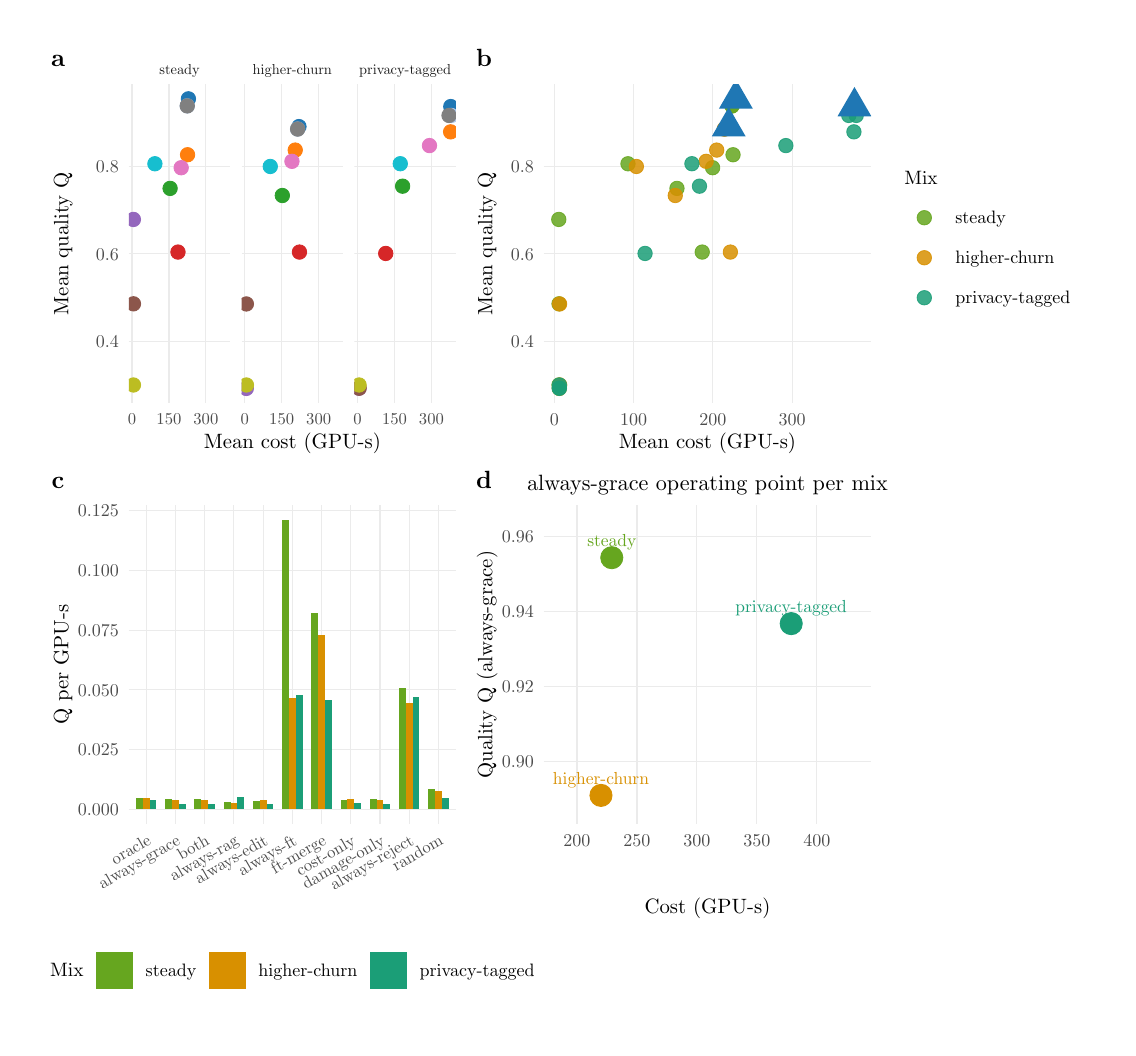
\begin{tikzpicture}[x=1pt,y=1pt]
\definecolor{fillColor}{RGB}{255,255,255}
\path[use as bounding box,fill=fillColor,fill opacity=0.00] (0,0) rectangle (390.26,361.35);
\begin{scope}
\path[clip] (  0.00,  0.00) rectangle (390.26,361.35);
\definecolor{drawColor}{RGB}{255,255,255}
\definecolor{fillColor}{RGB}{255,255,255}

\path[draw=drawColor,line width= 0.6pt,line join=round,line cap=round,fill=fillColor] (  0.00,  0.00) rectangle (390.26,361.35);
\end{scope}
\begin{scope}
\path[clip] (  5.50,203.79) rectangle (158.76,355.85);
\definecolor{fillColor}{RGB}{255,255,255}

\path[fill=fillColor] (  5.50,203.79) rectangle (158.76,355.85);
\end{scope}
\begin{scope}
\path[clip] (158.76,203.79) rectangle (384.76,355.85);
\definecolor{fillColor}{RGB}{255,255,255}

\path[fill=fillColor] (158.76,203.79) rectangle (384.76,355.85);
\end{scope}
\begin{scope}
\path[clip] (  5.50,  5.50) rectangle (158.76,203.79);
\definecolor{fillColor}{RGB}{255,255,255}

\path[fill=fillColor] (  5.50,  5.50) rectangle (158.76,203.79);
\end{scope}
\begin{scope}
\path[clip] (158.76,  5.50) rectangle (384.76,203.79);
\definecolor{fillColor}{RGB}{255,255,255}

\path[fill=fillColor] (158.76,  5.50) rectangle (384.76,203.79);
\end{scope}
\begin{scope}
\path[clip] ( 36.53,225.75) rectangle ( 73.27,340.86);
\definecolor{drawColor}{gray}{0.92}

\path[draw=drawColor,line width= 0.4pt,line join=round] ( 36.53,248.03) --
	( 73.27,248.03);

\path[draw=drawColor,line width= 0.4pt,line join=round] ( 36.53,279.63) --
	( 73.27,279.63);

\path[draw=drawColor,line width= 0.4pt,line join=round] ( 36.53,311.23) --
	( 73.27,311.23);

\path[draw=drawColor,line width= 0.4pt,line join=round] ( 37.70,225.75) --
	( 37.70,340.86);

\path[draw=drawColor,line width= 0.4pt,line join=round] ( 51.05,225.75) --
	( 51.05,340.86);

\path[draw=drawColor,line width= 0.4pt,line join=round] ( 64.40,225.75) --
	( 64.40,340.86);
\definecolor{drawColor}{RGB}{44,160,44}
\definecolor{fillColor}{RGB}{44,160,44}

\path[draw=drawColor,line width= 0.3pt,line join=round,line cap=round,fill=fillColor] ( 51.47,303.27) circle (  2.61);
\definecolor{drawColor}{RGB}{31,119,180}
\definecolor{fillColor}{RGB}{31,119,180}

\path[draw=drawColor,line width= 0.3pt,line join=round,line cap=round,fill=fillColor] ( 58.08,335.63) circle (  2.61);
\definecolor{drawColor}{RGB}{174,199,232}
\definecolor{fillColor}{RGB}{174,199,232}

\path[draw=drawColor,line width= 0.3pt,line join=round,line cap=round,fill=fillColor] ( 57.65,333.08) circle (  2.61);
\definecolor{drawColor}{RGB}{214,39,40}
\definecolor{fillColor}{RGB}{214,39,40}

\path[draw=drawColor,line width= 0.3pt,line join=round,line cap=round,fill=fillColor] ( 54.31,280.26) circle (  2.61);
\definecolor{drawColor}{RGB}{255,127,14}
\definecolor{fillColor}{RGB}{255,127,14}

\path[draw=drawColor,line width= 0.3pt,line join=round,line cap=round,fill=fillColor] ( 57.77,315.43) circle (  2.61);
\definecolor{drawColor}{RGB}{148,103,189}
\definecolor{fillColor}{RGB}{148,103,189}

\path[draw=drawColor,line width= 0.3pt,line join=round,line cap=round,fill=fillColor] ( 38.20,292.05) circle (  2.61);
\definecolor{drawColor}{RGB}{140,86,75}
\definecolor{fillColor}{RGB}{140,86,75}

\path[draw=drawColor,line width= 0.3pt,line join=round,line cap=round,fill=fillColor] ( 38.22,261.56) circle (  2.61);
\definecolor{drawColor}{RGB}{227,119,194}
\definecolor{fillColor}{RGB}{227,119,194}

\path[draw=drawColor,line width= 0.3pt,line join=round,line cap=round,fill=fillColor] ( 55.47,310.74) circle (  2.61);
\definecolor{drawColor}{gray}{0.50}
\definecolor{fillColor}{gray}{0.50}

\path[draw=drawColor,line width= 0.3pt,line join=round,line cap=round,fill=fillColor] ( 57.66,333.08) circle (  2.61);
\definecolor{drawColor}{RGB}{188,189,34}
\definecolor{fillColor}{RGB}{188,189,34}

\path[draw=drawColor,line width= 0.3pt,line join=round,line cap=round,fill=fillColor] ( 38.22,232.23) circle (  2.61);
\definecolor{drawColor}{RGB}{23,190,207}
\definecolor{fillColor}{RGB}{23,190,207}

\path[draw=drawColor,line width= 0.3pt,line join=round,line cap=round,fill=fillColor] ( 45.97,312.17) circle (  2.61);
\end{scope}
\begin{scope}
\path[clip] ( 77.27,225.75) rectangle (114.01,340.86);
\definecolor{drawColor}{gray}{0.92}

\path[draw=drawColor,line width= 0.4pt,line join=round] ( 77.27,248.03) --
	(114.01,248.03);

\path[draw=drawColor,line width= 0.4pt,line join=round] ( 77.27,279.63) --
	(114.01,279.63);

\path[draw=drawColor,line width= 0.4pt,line join=round] ( 77.27,311.23) --
	(114.01,311.23);

\path[draw=drawColor,line width= 0.4pt,line join=round] ( 78.44,225.75) --
	( 78.44,340.86);

\path[draw=drawColor,line width= 0.4pt,line join=round] ( 91.79,225.75) --
	( 91.79,340.86);

\path[draw=drawColor,line width= 0.4pt,line join=round] (105.15,225.75) --
	(105.15,340.86);
\definecolor{drawColor}{RGB}{44,160,44}
\definecolor{fillColor}{RGB}{44,160,44}

\path[draw=drawColor,line width= 0.3pt,line join=round,line cap=round,fill=fillColor] ( 92.02,300.70) circle (  2.61);
\definecolor{drawColor}{RGB}{31,119,180}
\definecolor{fillColor}{RGB}{31,119,180}

\path[draw=drawColor,line width= 0.3pt,line join=round,line cap=round,fill=fillColor] ( 98.03,325.60) circle (  2.61);
\definecolor{drawColor}{RGB}{174,199,232}
\definecolor{fillColor}{RGB}{174,199,232}

\path[draw=drawColor,line width= 0.3pt,line join=round,line cap=round,fill=fillColor] ( 97.52,324.71) circle (  2.61);
\definecolor{drawColor}{RGB}{214,39,40}
\definecolor{fillColor}{RGB}{214,39,40}

\path[draw=drawColor,line width= 0.3pt,line join=round,line cap=round,fill=fillColor] ( 98.21,280.26) circle (  2.61);
\definecolor{drawColor}{RGB}{255,127,14}
\definecolor{fillColor}{RGB}{255,127,14}

\path[draw=drawColor,line width= 0.3pt,line join=round,line cap=round,fill=fillColor] ( 96.68,317.11) circle (  2.61);
\definecolor{drawColor}{RGB}{148,103,189}
\definecolor{fillColor}{RGB}{148,103,189}

\path[draw=drawColor,line width= 0.3pt,line join=round,line cap=round,fill=fillColor] ( 79.00,230.99) circle (  2.61);
\definecolor{drawColor}{RGB}{140,86,75}
\definecolor{fillColor}{RGB}{140,86,75}

\path[draw=drawColor,line width= 0.3pt,line join=round,line cap=round,fill=fillColor] ( 79.03,261.51) circle (  2.61);
\definecolor{drawColor}{RGB}{227,119,194}
\definecolor{fillColor}{RGB}{227,119,194}

\path[draw=drawColor,line width= 0.3pt,line join=round,line cap=round,fill=fillColor] ( 95.49,313.05) circle (  2.61);
\definecolor{drawColor}{gray}{0.50}
\definecolor{fillColor}{gray}{0.50}

\path[draw=drawColor,line width= 0.3pt,line join=round,line cap=round,fill=fillColor] ( 97.55,324.71) circle (  2.61);
\definecolor{drawColor}{RGB}{188,189,34}
\definecolor{fillColor}{RGB}{188,189,34}

\path[draw=drawColor,line width= 0.3pt,line join=round,line cap=round,fill=fillColor] ( 79.04,232.23) circle (  2.61);
\definecolor{drawColor}{RGB}{23,190,207}
\definecolor{fillColor}{RGB}{23,190,207}

\path[draw=drawColor,line width= 0.3pt,line join=round,line cap=round,fill=fillColor] ( 87.66,311.19) circle (  2.61);
\end{scope}
\begin{scope}
\path[clip] (118.01,225.75) rectangle (154.76,340.86);
\definecolor{drawColor}{gray}{0.92}

\path[draw=drawColor,line width= 0.4pt,line join=round] (118.01,248.03) --
	(154.76,248.03);

\path[draw=drawColor,line width= 0.4pt,line join=round] (118.01,279.63) --
	(154.76,279.63);

\path[draw=drawColor,line width= 0.4pt,line join=round] (118.01,311.23) --
	(154.76,311.23);

\path[draw=drawColor,line width= 0.4pt,line join=round] (119.19,225.75) --
	(119.19,340.86);

\path[draw=drawColor,line width= 0.4pt,line join=round] (132.54,225.75) --
	(132.54,340.86);

\path[draw=drawColor,line width= 0.4pt,line join=round] (145.89,225.75) --
	(145.89,340.86);
\definecolor{drawColor}{RGB}{44,160,44}
\definecolor{fillColor}{RGB}{44,160,44}

\path[draw=drawColor,line width= 0.3pt,line join=round,line cap=round,fill=fillColor] (135.48,304.07) circle (  2.61);
\definecolor{drawColor}{RGB}{31,119,180}
\definecolor{fillColor}{RGB}{31,119,180}

\path[draw=drawColor,line width= 0.3pt,line join=round,line cap=round,fill=fillColor] (152.89,332.84) circle (  2.61);
\definecolor{drawColor}{RGB}{174,199,232}
\definecolor{fillColor}{RGB}{174,199,232}

\path[draw=drawColor,line width= 0.3pt,line join=round,line cap=round,fill=fillColor] (153.09,329.63) circle (  2.61);
\definecolor{drawColor}{RGB}{214,39,40}
\definecolor{fillColor}{RGB}{214,39,40}

\path[draw=drawColor,line width= 0.3pt,line join=round,line cap=round,fill=fillColor] (129.38,279.76) circle (  2.61);
\definecolor{drawColor}{RGB}{255,127,14}
\definecolor{fillColor}{RGB}{255,127,14}

\path[draw=drawColor,line width= 0.3pt,line join=round,line cap=round,fill=fillColor] (152.83,323.70) circle (  2.61);
\definecolor{drawColor}{RGB}{148,103,189}
\definecolor{fillColor}{RGB}{148,103,189}

\path[draw=drawColor,line width= 0.3pt,line join=round,line cap=round,fill=fillColor] (119.73,231.07) circle (  2.61);
\definecolor{drawColor}{RGB}{140,86,75}
\definecolor{fillColor}{RGB}{140,86,75}

\path[draw=drawColor,line width= 0.3pt,line join=round,line cap=round,fill=fillColor] (119.76,231.07) circle (  2.61);
\definecolor{drawColor}{RGB}{227,119,194}
\definecolor{fillColor}{RGB}{227,119,194}

\path[draw=drawColor,line width= 0.3pt,line join=round,line cap=round,fill=fillColor] (145.19,318.74) circle (  2.61);
\definecolor{drawColor}{gray}{0.50}
\definecolor{fillColor}{gray}{0.50}

\path[draw=drawColor,line width= 0.3pt,line join=round,line cap=round,fill=fillColor] (152.25,329.63) circle (  2.61);
\definecolor{drawColor}{RGB}{188,189,34}
\definecolor{fillColor}{RGB}{188,189,34}

\path[draw=drawColor,line width= 0.3pt,line join=round,line cap=round,fill=fillColor] (119.76,232.23) circle (  2.61);
\definecolor{drawColor}{RGB}{23,190,207}
\definecolor{fillColor}{RGB}{23,190,207}

\path[draw=drawColor,line width= 0.3pt,line join=round,line cap=round,fill=fillColor] (134.64,312.19) circle (  2.61);
\end{scope}
\begin{scope}
\path[clip] (  0.00,  0.00) rectangle (390.26,361.35);
\definecolor{drawColor}{gray}{0.10}

\node[text=drawColor,anchor=base,inner sep=0pt, outer sep=0pt, scale=  0.52] at ( 54.90,344.56) {steady};
\end{scope}
\begin{scope}
\path[clip] (  0.00,  0.00) rectangle (390.26,361.35);
\definecolor{drawColor}{gray}{0.10}

\node[text=drawColor,anchor=base,inner sep=0pt, outer sep=0pt, scale=  0.52] at ( 95.64,344.56) {higher-churn};
\end{scope}
\begin{scope}
\path[clip] (  0.00,  0.00) rectangle (390.26,361.35);
\definecolor{drawColor}{gray}{0.10}

\node[text=drawColor,anchor=base,inner sep=0pt, outer sep=0pt, scale=  0.52] at (136.39,344.56) {privacy-tagged};
\end{scope}
\begin{scope}
\path[clip] (  0.00,  0.00) rectangle (390.26,361.35);
\definecolor{drawColor}{gray}{0.30}

\node[text=drawColor,anchor=base,inner sep=0pt, outer sep=0pt, scale=  0.60] at ( 37.70,218.02) {0};

\node[text=drawColor,anchor=base,inner sep=0pt, outer sep=0pt, scale=  0.60] at ( 51.05,218.02) {150};

\node[text=drawColor,anchor=base,inner sep=0pt, outer sep=0pt, scale=  0.60] at ( 64.40,218.02) {300};
\end{scope}
\begin{scope}
\path[clip] (  0.00,  0.00) rectangle (390.26,361.35);
\definecolor{drawColor}{gray}{0.30}

\node[text=drawColor,anchor=base,inner sep=0pt, outer sep=0pt, scale=  0.60] at ( 78.44,218.02) {0};

\node[text=drawColor,anchor=base,inner sep=0pt, outer sep=0pt, scale=  0.60] at ( 91.79,218.02) {150};

\node[text=drawColor,anchor=base,inner sep=0pt, outer sep=0pt, scale=  0.60] at (105.15,218.02) {300};
\end{scope}
\begin{scope}
\path[clip] (  0.00,  0.00) rectangle (390.26,361.35);
\definecolor{drawColor}{gray}{0.30}

\node[text=drawColor,anchor=base,inner sep=0pt, outer sep=0pt, scale=  0.60] at (119.19,218.02) {0};

\node[text=drawColor,anchor=base,inner sep=0pt, outer sep=0pt, scale=  0.60] at (132.54,218.02) {150};

\node[text=drawColor,anchor=base,inner sep=0pt, outer sep=0pt, scale=  0.60] at (145.89,218.02) {300};
\end{scope}
\begin{scope}
\path[clip] (  0.00,  0.00) rectangle (390.26,361.35);
\definecolor{drawColor}{gray}{0.30}

\node[text=drawColor,anchor=base east,inner sep=0pt, outer sep=0pt, scale=  0.65] at ( 32.93,245.79) {0.4};

\node[text=drawColor,anchor=base east,inner sep=0pt, outer sep=0pt, scale=  0.65] at ( 32.93,277.39) {0.6};

\node[text=drawColor,anchor=base east,inner sep=0pt, outer sep=0pt, scale=  0.65] at ( 32.93,308.99) {0.8};
\end{scope}
\begin{scope}
\path[clip] (  0.00,  0.00) rectangle (390.26,361.35);
\definecolor{drawColor}{RGB}{0,0,0}

\node[text=drawColor,anchor=base,inner sep=0pt, outer sep=0pt, scale=  0.75] at ( 95.64,209.25) {Mean cost (GPU-s)};
\end{scope}
\begin{scope}
\path[clip] (  0.00,  0.00) rectangle (390.26,361.35);
\definecolor{drawColor}{RGB}{0,0,0}

\node[text=drawColor,rotate= 90.00,anchor=base,inner sep=0pt, outer sep=0pt, scale=  0.75] at ( 14.67,283.31) {Mean quality Q};
\end{scope}
\begin{scope}
\path[clip] (  0.00,  0.00) rectangle (390.26,361.35);
\definecolor{drawColor}{RGB}{0,0,0}

\node[text=drawColor,anchor=base,inner sep=0pt, outer sep=0pt, scale=  0.90] at ( 10.95,347.30) {\bfseries a};
\end{scope}
\begin{scope}
\path[clip] (186.53,225.75) rectangle (304.77,340.86);
\definecolor{drawColor}{gray}{0.92}

\path[draw=drawColor,line width= 0.4pt,line join=round] (186.53,248.03) --
	(304.77,248.03);

\path[draw=drawColor,line width= 0.4pt,line join=round] (186.53,279.63) --
	(304.77,279.63);

\path[draw=drawColor,line width= 0.4pt,line join=round] (186.53,311.23) --
	(304.77,311.23);

\path[draw=drawColor,line width= 0.4pt,line join=round] (190.30,225.75) --
	(190.30,340.86);

\path[draw=drawColor,line width= 0.4pt,line join=round] (218.95,225.75) --
	(218.95,340.86);

\path[draw=drawColor,line width= 0.4pt,line join=round] (247.60,225.75) --
	(247.60,340.86);

\path[draw=drawColor,line width= 0.4pt,line join=round] (276.24,225.75) --
	(276.24,340.86);
\definecolor{drawColor}{RGB}{102,166,31}
\definecolor{fillColor}{RGB}{102,166,31}

\path[draw=drawColor,draw opacity=0.85,line width= 0.3pt,line join=round,line cap=round,fill=fillColor,fill opacity=0.85] (234.62,303.27) circle (  2.61);

\path[draw=drawColor,draw opacity=0.85,line width= 0.3pt,line join=round,line cap=round,fill=fillColor,fill opacity=0.85] (255.91,335.63) circle (  2.61);

\path[draw=drawColor,draw opacity=0.85,line width= 0.3pt,line join=round,line cap=round,fill=fillColor,fill opacity=0.85] (254.49,333.08) circle (  2.61);

\path[draw=drawColor,draw opacity=0.85,line width= 0.3pt,line join=round,line cap=round,fill=fillColor,fill opacity=0.85] (243.75,280.26) circle (  2.61);

\path[draw=drawColor,draw opacity=0.85,line width= 0.3pt,line join=round,line cap=round,fill=fillColor,fill opacity=0.85] (254.88,315.43) circle (  2.61);

\path[draw=drawColor,draw opacity=0.85,line width= 0.3pt,line join=round,line cap=round,fill=fillColor,fill opacity=0.85] (191.91,292.05) circle (  2.61);

\path[draw=drawColor,draw opacity=0.85,line width= 0.3pt,line join=round,line cap=round,fill=fillColor,fill opacity=0.85] (192.00,261.56) circle (  2.61);

\path[draw=drawColor,draw opacity=0.85,line width= 0.3pt,line join=round,line cap=round,fill=fillColor,fill opacity=0.85] (247.50,310.74) circle (  2.61);

\path[draw=drawColor,draw opacity=0.85,line width= 0.3pt,line join=round,line cap=round,fill=fillColor,fill opacity=0.85] (254.55,333.08) circle (  2.61);

\path[draw=drawColor,draw opacity=0.85,line width= 0.3pt,line join=round,line cap=round,fill=fillColor,fill opacity=0.85] (191.99,232.23) circle (  2.61);

\path[draw=drawColor,draw opacity=0.85,line width= 0.3pt,line join=round,line cap=round,fill=fillColor,fill opacity=0.85] (216.92,312.17) circle (  2.61);
\definecolor{drawColor}{RGB}{216,144,0}
\definecolor{fillColor}{RGB}{216,144,0}

\path[draw=drawColor,draw opacity=0.85,line width= 0.3pt,line join=round,line cap=round,fill=fillColor,fill opacity=0.85] (234.00,300.70) circle (  2.61);

\path[draw=drawColor,draw opacity=0.85,line width= 0.3pt,line join=round,line cap=round,fill=fillColor,fill opacity=0.85] (253.33,325.60) circle (  2.61);

\path[draw=drawColor,draw opacity=0.85,line width= 0.3pt,line join=round,line cap=round,fill=fillColor,fill opacity=0.85] (251.71,324.71) circle (  2.61);

\path[draw=drawColor,draw opacity=0.85,line width= 0.3pt,line join=round,line cap=round,fill=fillColor,fill opacity=0.85] (253.92,280.26) circle (  2.61);

\path[draw=drawColor,draw opacity=0.85,line width= 0.3pt,line join=round,line cap=round,fill=fillColor,fill opacity=0.85] (248.98,317.11) circle (  2.61);

\path[draw=drawColor,draw opacity=0.85,line width= 0.3pt,line join=round,line cap=round,fill=fillColor,fill opacity=0.85] (192.10,230.99) circle (  2.61);

\path[draw=drawColor,draw opacity=0.85,line width= 0.3pt,line join=round,line cap=round,fill=fillColor,fill opacity=0.85] (192.21,261.51) circle (  2.61);

\path[draw=drawColor,draw opacity=0.85,line width= 0.3pt,line join=round,line cap=round,fill=fillColor,fill opacity=0.85] (245.16,313.05) circle (  2.61);

\path[draw=drawColor,draw opacity=0.85,line width= 0.3pt,line join=round,line cap=round,fill=fillColor,fill opacity=0.85] (251.80,324.71) circle (  2.61);

\path[draw=drawColor,draw opacity=0.85,line width= 0.3pt,line join=round,line cap=round,fill=fillColor,fill opacity=0.85] (192.23,232.23) circle (  2.61);

\path[draw=drawColor,draw opacity=0.85,line width= 0.3pt,line join=round,line cap=round,fill=fillColor,fill opacity=0.85] (219.95,311.19) circle (  2.61);
\definecolor{drawColor}{RGB}{27,158,119}
\definecolor{fillColor}{RGB}{27,158,119}

\path[draw=drawColor,draw opacity=0.85,line width= 0.3pt,line join=round,line cap=round,fill=fillColor,fill opacity=0.85] (242.75,304.07) circle (  2.61);

\path[draw=drawColor,draw opacity=0.85,line width= 0.3pt,line join=round,line cap=round,fill=fillColor,fill opacity=0.85] (298.76,332.84) circle (  2.61);

\path[draw=drawColor,draw opacity=0.85,line width= 0.3pt,line join=round,line cap=round,fill=fillColor,fill opacity=0.85] (299.39,329.63) circle (  2.61);

\path[draw=drawColor,draw opacity=0.85,line width= 0.3pt,line join=round,line cap=round,fill=fillColor,fill opacity=0.85] (223.09,279.76) circle (  2.61);

\path[draw=drawColor,draw opacity=0.85,line width= 0.3pt,line join=round,line cap=round,fill=fillColor,fill opacity=0.85] (298.56,323.70) circle (  2.61);

\path[draw=drawColor,draw opacity=0.85,line width= 0.3pt,line join=round,line cap=round,fill=fillColor,fill opacity=0.85] (192.06,231.07) circle (  2.61);

\path[draw=drawColor,draw opacity=0.85,line width= 0.3pt,line join=round,line cap=round,fill=fillColor,fill opacity=0.85] (192.14,231.07) circle (  2.61);

\path[draw=drawColor,draw opacity=0.85,line width= 0.3pt,line join=round,line cap=round,fill=fillColor,fill opacity=0.85] (273.97,318.74) circle (  2.61);

\path[draw=drawColor,draw opacity=0.85,line width= 0.3pt,line join=round,line cap=round,fill=fillColor,fill opacity=0.85] (296.70,329.63) circle (  2.61);

\path[draw=drawColor,draw opacity=0.85,line width= 0.3pt,line join=round,line cap=round,fill=fillColor,fill opacity=0.85] (192.14,232.23) circle (  2.61);

\path[draw=drawColor,draw opacity=0.85,line width= 0.3pt,line join=round,line cap=round,fill=fillColor,fill opacity=0.85] (240.02,312.19) circle (  2.61);
\definecolor{fillColor}{RGB}{31,119,180}

\path[fill=fillColor] (255.91,342.69) --
	(262.02,332.09) --
	(249.79,332.09) --
	cycle;

\path[fill=fillColor] (253.33,332.66) --
	(259.44,322.06) --
	(247.21,322.06) --
	cycle;

\path[fill=fillColor] (298.76,339.91) --
	(304.88,329.31) --
	(292.64,329.31) --
	cycle;
\end{scope}
\begin{scope}
\path[clip] (  0.00,  0.00) rectangle (390.26,361.35);
\definecolor{drawColor}{gray}{0.30}

\node[text=drawColor,anchor=base east,inner sep=0pt, outer sep=0pt, scale=  0.65] at (182.93,245.79) {0.4};

\node[text=drawColor,anchor=base east,inner sep=0pt, outer sep=0pt, scale=  0.65] at (182.93,277.39) {0.6};

\node[text=drawColor,anchor=base east,inner sep=0pt, outer sep=0pt, scale=  0.65] at (182.93,308.99) {0.8};
\end{scope}
\begin{scope}
\path[clip] (  0.00,  0.00) rectangle (390.26,361.35);
\definecolor{drawColor}{gray}{0.30}

\node[text=drawColor,anchor=base,inner sep=0pt, outer sep=0pt, scale=  0.65] at (190.30,217.68) {0};

\node[text=drawColor,anchor=base,inner sep=0pt, outer sep=0pt, scale=  0.65] at (218.95,217.68) {100};

\node[text=drawColor,anchor=base,inner sep=0pt, outer sep=0pt, scale=  0.65] at (247.60,217.68) {200};

\node[text=drawColor,anchor=base,inner sep=0pt, outer sep=0pt, scale=  0.65] at (276.24,217.68) {300};
\end{scope}
\begin{scope}
\path[clip] (  0.00,  0.00) rectangle (390.26,361.35);
\definecolor{drawColor}{RGB}{0,0,0}

\node[text=drawColor,anchor=base,inner sep=0pt, outer sep=0pt, scale=  0.75] at (245.65,209.25) {Mean cost (GPU-s)};
\end{scope}
\begin{scope}
\path[clip] (  0.00,  0.00) rectangle (390.26,361.35);
\definecolor{drawColor}{RGB}{0,0,0}

\node[text=drawColor,rotate= 90.00,anchor=base,inner sep=0pt, outer sep=0pt, scale=  0.75] at (167.92,283.31) {Mean quality Q};
\end{scope}
\begin{scope}
\path[clip] (  0.00,  0.00) rectangle (390.26,361.35);
\definecolor{drawColor}{RGB}{0,0,0}

\node[text=drawColor,anchor=base west,inner sep=0pt, outer sep=0pt, scale=  0.70] at (316.77,304.58) {Mix};
\end{scope}
\begin{scope}
\path[clip] (  0.00,  0.00) rectangle (390.26,361.35);
\definecolor{drawColor}{RGB}{102,166,31}
\definecolor{fillColor}{RGB}{102,166,31}

\path[draw=drawColor,draw opacity=0.85,line width= 0.3pt,line join=round,line cap=round,fill=fillColor,fill opacity=0.85] (324.00,292.67) circle (  2.61);
\end{scope}
\begin{scope}
\path[clip] (  0.00,  0.00) rectangle (390.26,361.35);
\definecolor{drawColor}{RGB}{216,144,0}
\definecolor{fillColor}{RGB}{216,144,0}

\path[draw=drawColor,draw opacity=0.85,line width= 0.3pt,line join=round,line cap=round,fill=fillColor,fill opacity=0.85] (324.00,278.21) circle (  2.61);
\end{scope}
\begin{scope}
\path[clip] (  0.00,  0.00) rectangle (390.26,361.35);
\definecolor{drawColor}{RGB}{27,158,119}
\definecolor{fillColor}{RGB}{27,158,119}

\path[draw=drawColor,draw opacity=0.85,line width= 0.3pt,line join=round,line cap=round,fill=fillColor,fill opacity=0.85] (324.00,263.76) circle (  2.61);
\end{scope}
\begin{scope}
\path[clip] (  0.00,  0.00) rectangle (390.26,361.35);
\definecolor{drawColor}{RGB}{0,0,0}

\node[text=drawColor,anchor=base west,inner sep=0pt, outer sep=0pt, scale=  0.65] at (335.22,290.43) {steady};
\end{scope}
\begin{scope}
\path[clip] (  0.00,  0.00) rectangle (390.26,361.35);
\definecolor{drawColor}{RGB}{0,0,0}

\node[text=drawColor,anchor=base west,inner sep=0pt, outer sep=0pt, scale=  0.65] at (335.22,275.98) {higher-churn};
\end{scope}
\begin{scope}
\path[clip] (  0.00,  0.00) rectangle (390.26,361.35);
\definecolor{drawColor}{RGB}{0,0,0}

\node[text=drawColor,anchor=base west,inner sep=0pt, outer sep=0pt, scale=  0.65] at (335.22,261.52) {privacy-tagged};
\end{scope}
\begin{scope}
\path[clip] (  0.00,  0.00) rectangle (390.26,361.35);
\definecolor{drawColor}{RGB}{0,0,0}

\node[text=drawColor,anchor=base,inner sep=0pt, outer sep=0pt, scale=  0.90] at (164.94,347.30) {\bfseries b};
\end{scope}
\begin{scope}
\path[clip] ( 36.53, 73.62) rectangle (154.76,188.72);
\definecolor{drawColor}{gray}{0.92}

\path[draw=drawColor,line width= 0.4pt,line join=round] ( 36.53, 78.85) --
	(154.76, 78.85);

\path[draw=drawColor,line width= 0.4pt,line join=round] ( 36.53,100.45) --
	(154.76,100.45);

\path[draw=drawColor,line width= 0.4pt,line join=round] ( 36.53,122.05) --
	(154.76,122.05);

\path[draw=drawColor,line width= 0.4pt,line join=round] ( 36.53,143.65) --
	(154.76,143.65);

\path[draw=drawColor,line width= 0.4pt,line join=round] ( 36.53,165.25) --
	(154.76,165.25);

\path[draw=drawColor,line width= 0.4pt,line join=round] ( 36.53,186.84) --
	(154.76,186.84);

\path[draw=drawColor,line width= 0.4pt,line join=round] ( 42.86, 73.62) --
	( 42.86,188.72);

\path[draw=drawColor,line width= 0.4pt,line join=round] ( 53.42, 73.62) --
	( 53.42,188.72);

\path[draw=drawColor,line width= 0.4pt,line join=round] ( 63.97, 73.62) --
	( 63.97,188.72);

\path[draw=drawColor,line width= 0.4pt,line join=round] ( 74.53, 73.62) --
	( 74.53,188.72);

\path[draw=drawColor,line width= 0.4pt,line join=round] ( 85.09, 73.62) --
	( 85.09,188.72);

\path[draw=drawColor,line width= 0.4pt,line join=round] ( 95.64, 73.62) --
	( 95.64,188.72);

\path[draw=drawColor,line width= 0.4pt,line join=round] (106.20, 73.62) --
	(106.20,188.72);

\path[draw=drawColor,line width= 0.4pt,line join=round] (116.76, 73.62) --
	(116.76,188.72);

\path[draw=drawColor,line width= 0.4pt,line join=round] (127.31, 73.62) --
	(127.31,188.72);

\path[draw=drawColor,line width= 0.4pt,line join=round] (137.87, 73.62) --
	(137.87,188.72);

\path[draw=drawColor,line width= 0.4pt,line join=round] (148.42, 73.62) --
	(148.42,188.72);
\definecolor{fillColor}{RGB}{102,166,31}

\path[fill=fillColor] ( 39.16, 78.85) rectangle ( 41.63, 83.04);

\path[fill=fillColor] ( 49.72, 78.85) rectangle ( 52.18, 82.45);

\path[fill=fillColor] ( 60.28, 78.85) rectangle ( 62.74, 82.47);

\path[fill=fillColor] ( 70.83, 78.85) rectangle ( 73.30, 81.65);

\path[fill=fillColor] ( 81.39, 78.85) rectangle ( 83.85, 82.02);

\path[fill=fillColor] ( 91.95, 78.85) rectangle ( 94.41,183.49);

\path[fill=fillColor] (102.50, 78.85) rectangle (104.97,149.92);

\path[fill=fillColor] (113.06, 78.85) rectangle (115.52, 82.30);

\path[fill=fillColor] (123.62, 78.85) rectangle (126.08, 82.47);

\path[fill=fillColor] (134.17, 78.85) rectangle (136.64,122.77);

\path[fill=fillColor] (144.73, 78.85) rectangle (147.19, 86.35);
\definecolor{fillColor}{RGB}{216,144,0}

\path[fill=fillColor] ( 41.63, 78.85) rectangle ( 44.09, 83.01);

\path[fill=fillColor] ( 52.18, 78.85) rectangle ( 54.65, 82.35);

\path[fill=fillColor] ( 62.74, 78.85) rectangle ( 65.20, 82.42);

\path[fill=fillColor] ( 73.30, 78.85) rectangle ( 75.76, 81.20);

\path[fill=fillColor] ( 83.85, 78.85) rectangle ( 86.32, 82.38);

\path[fill=fillColor] ( 94.41, 78.85) rectangle ( 96.87,119.19);

\path[fill=fillColor] (104.97, 78.85) rectangle (107.43,141.99);

\path[fill=fillColor] (115.52, 78.85) rectangle (117.99, 82.51);

\path[fill=fillColor] (126.08, 78.85) rectangle (128.54, 82.42);

\path[fill=fillColor] (136.64, 78.85) rectangle (139.10,117.37);

\path[fill=fillColor] (147.19, 78.85) rectangle (149.66, 85.53);
\definecolor{fillColor}{RGB}{27,158,119}

\path[fill=fillColor] ( 44.09, 78.85) rectangle ( 46.55, 82.41);

\path[fill=fillColor] ( 54.65, 78.85) rectangle ( 57.11, 80.99);

\path[fill=fillColor] ( 65.20, 78.85) rectangle ( 67.67, 80.93);

\path[fill=fillColor] ( 75.76, 78.85) rectangle ( 78.22, 83.39);

\path[fill=fillColor] ( 86.32, 78.85) rectangle ( 88.78, 80.86);

\path[fill=fillColor] ( 96.87, 78.85) rectangle ( 99.34,120.20);

\path[fill=fillColor] (107.43, 78.85) rectangle (109.89,118.34);

\path[fill=fillColor] (117.99, 78.85) rectangle (120.45, 81.36);

\path[fill=fillColor] (128.54, 78.85) rectangle (131.01, 80.98);

\path[fill=fillColor] (139.10, 78.85) rectangle (141.56,119.31);

\path[fill=fillColor] (149.66, 78.85) rectangle (152.12, 82.87);
\end{scope}
\begin{scope}
\path[clip] (  0.00,  0.00) rectangle (390.26,361.35);
\definecolor{drawColor}{gray}{0.30}

\node[text=drawColor,anchor=base east,inner sep=0pt, outer sep=0pt, scale=  0.65] at ( 32.93, 76.61) {0.000};

\node[text=drawColor,anchor=base east,inner sep=0pt, outer sep=0pt, scale=  0.65] at ( 32.93, 98.21) {0.025};

\node[text=drawColor,anchor=base east,inner sep=0pt, outer sep=0pt, scale=  0.65] at ( 32.93,119.81) {0.050};

\node[text=drawColor,anchor=base east,inner sep=0pt, outer sep=0pt, scale=  0.65] at ( 32.93,141.41) {0.075};

\node[text=drawColor,anchor=base east,inner sep=0pt, outer sep=0pt, scale=  0.65] at ( 32.93,163.01) {0.100};

\node[text=drawColor,anchor=base east,inner sep=0pt, outer sep=0pt, scale=  0.65] at ( 32.93,184.60) {0.125};
\end{scope}
\begin{scope}
\path[clip] (  0.00,  0.00) rectangle (390.26,361.35);
\definecolor{drawColor}{gray}{0.30}

\node[text=drawColor,rotate= 30.00,anchor=base east,inner sep=0pt, outer sep=0pt, scale=  0.60] at ( 44.93, 66.44) {oracle};

\node[text=drawColor,rotate= 30.00,anchor=base east,inner sep=0pt, outer sep=0pt, scale=  0.60] at ( 55.48, 66.44) {always-grace};

\node[text=drawColor,rotate= 30.00,anchor=base east,inner sep=0pt, outer sep=0pt, scale=  0.60] at ( 66.04, 66.44) {both};

\node[text=drawColor,rotate= 30.00,anchor=base east,inner sep=0pt, outer sep=0pt, scale=  0.60] at ( 76.60, 66.44) {always-rag};

\node[text=drawColor,rotate= 30.00,anchor=base east,inner sep=0pt, outer sep=0pt, scale=  0.60] at ( 87.15, 66.44) {always-edit};

\node[text=drawColor,rotate= 30.00,anchor=base east,inner sep=0pt, outer sep=0pt, scale=  0.60] at ( 97.71, 66.44) {always-ft};

\node[text=drawColor,rotate= 30.00,anchor=base east,inner sep=0pt, outer sep=0pt, scale=  0.60] at (108.26, 66.44) {ft-merge};

\node[text=drawColor,rotate= 30.00,anchor=base east,inner sep=0pt, outer sep=0pt, scale=  0.60] at (118.82, 66.44) {cost-only};

\node[text=drawColor,rotate= 30.00,anchor=base east,inner sep=0pt, outer sep=0pt, scale=  0.60] at (129.38, 66.44) {damage-only};

\node[text=drawColor,rotate= 30.00,anchor=base east,inner sep=0pt, outer sep=0pt, scale=  0.60] at (139.93, 66.44) {always-reject};

\node[text=drawColor,rotate= 30.00,anchor=base east,inner sep=0pt, outer sep=0pt, scale=  0.60] at (150.49, 66.44) {random};
\end{scope}
\begin{scope}
\path[clip] (  0.00,  0.00) rectangle (390.26,361.35);
\definecolor{drawColor}{RGB}{0,0,0}

\node[text=drawColor,rotate= 90.00,anchor=base,inner sep=0pt, outer sep=0pt, scale=  0.75] at ( 14.67,131.17) {Q per GPU-s};
\end{scope}
\begin{scope}
\path[clip] (  0.00,  0.00) rectangle (390.26,361.35);
\definecolor{drawColor}{RGB}{0,0,0}

\node[text=drawColor,anchor=base west,inner sep=0pt, outer sep=0pt, scale=  0.70] at (  8.14, 18.32) {Mix};
\end{scope}
\begin{scope}
\path[clip] (  0.00,  0.00) rectangle (390.26,361.35);
\definecolor{fillColor}{RGB}{102,166,31}

\path[fill=fillColor] ( 24.71, 14.02) rectangle ( 38.13, 27.44);
\end{scope}
\begin{scope}
\path[clip] (  0.00,  0.00) rectangle (390.26,361.35);
\definecolor{fillColor}{RGB}{216,144,0}

\path[fill=fillColor] ( 65.44, 14.02) rectangle ( 78.86, 27.44);
\end{scope}
\begin{scope}
\path[clip] (  0.00,  0.00) rectangle (390.26,361.35);
\definecolor{fillColor}{RGB}{27,158,119}

\path[fill=fillColor] (123.67, 14.02) rectangle (137.09, 27.44);
\end{scope}
\begin{scope}
\path[clip] (  0.00,  0.00) rectangle (390.26,361.35);
\definecolor{drawColor}{RGB}{0,0,0}

\node[text=drawColor,anchor=base west,inner sep=0pt, outer sep=0pt, scale=  0.65] at ( 42.65, 18.49) {steady};
\end{scope}
\begin{scope}
\path[clip] (  0.00,  0.00) rectangle (390.26,361.35);
\definecolor{drawColor}{RGB}{0,0,0}

\node[text=drawColor,anchor=base west,inner sep=0pt, outer sep=0pt, scale=  0.65] at ( 83.37, 18.49) {higher-churn};
\end{scope}
\begin{scope}
\path[clip] (  0.00,  0.00) rectangle (390.26,361.35);
\definecolor{drawColor}{RGB}{0,0,0}

\node[text=drawColor,anchor=base west,inner sep=0pt, outer sep=0pt, scale=  0.65] at (141.60, 18.49) {privacy-tagged};
\end{scope}
\begin{scope}
\path[clip] (  0.00,  0.00) rectangle (390.26,361.35);
\definecolor{drawColor}{RGB}{0,0,0}

\node[text=drawColor,anchor=base,inner sep=0pt, outer sep=0pt, scale=  0.90] at ( 10.95,194.78) {\bfseries c};
\end{scope}
\begin{scope}
\path[clip] (186.53, 73.62) rectangle (304.77,188.72);
\definecolor{drawColor}{gray}{0.92}

\path[draw=drawColor,line width= 0.4pt,line join=round] (186.53, 96.22) --
	(304.77, 96.22);

\path[draw=drawColor,line width= 0.4pt,line join=round] (186.53,123.28) --
	(304.77,123.28);

\path[draw=drawColor,line width= 0.4pt,line join=round] (186.53,150.34) --
	(304.77,150.34);

\path[draw=drawColor,line width= 0.4pt,line join=round] (186.53,177.40) --
	(304.77,177.40);

\path[draw=drawColor,line width= 0.4pt,line join=round] (198.48, 73.62) --
	(198.48,188.72);

\path[draw=drawColor,line width= 0.4pt,line join=round] (220.16, 73.62) --
	(220.16,188.72);

\path[draw=drawColor,line width= 0.4pt,line join=round] (241.83, 73.62) --
	(241.83,188.72);

\path[draw=drawColor,line width= 0.4pt,line join=round] (263.50, 73.62) --
	(263.50,188.72);

\path[draw=drawColor,line width= 0.4pt,line join=round] (285.17, 73.62) --
	(285.17,188.72);
\definecolor{drawColor}{RGB}{102,166,31}
\definecolor{fillColor}{RGB}{102,166,31}

\path[draw=drawColor,line width= 0.3pt,line join=round,line cap=round,fill=fillColor] (211.06,169.83) circle (  4.01);
\definecolor{drawColor}{RGB}{216,144,0}
\definecolor{fillColor}{RGB}{216,144,0}

\path[draw=drawColor,line width= 0.3pt,line join=round,line cap=round,fill=fillColor] (207.16, 83.93) circle (  4.01);
\definecolor{drawColor}{RGB}{27,158,119}
\definecolor{fillColor}{RGB}{27,158,119}

\path[draw=drawColor,line width= 0.3pt,line join=round,line cap=round,fill=fillColor] (275.90,146.01) circle (  4.01);
\definecolor{drawColor}{RGB}{102,166,31}

\node[text=drawColor,anchor=base,inner sep=0pt, outer sep=0pt, scale=  0.63] at (211.06,173.71) {steady};
\definecolor{drawColor}{RGB}{216,144,0}

\node[text=drawColor,anchor=base,inner sep=0pt, outer sep=0pt, scale=  0.63] at (207.16, 87.81) {higher-churn};
\definecolor{drawColor}{RGB}{27,158,119}

\node[text=drawColor,anchor=base,inner sep=0pt, outer sep=0pt, scale=  0.63] at (275.90,149.89) {privacy-tagged};
\end{scope}
\begin{scope}
\path[clip] (  0.00,  0.00) rectangle (390.26,361.35);
\definecolor{drawColor}{gray}{0.30}

\node[text=drawColor,anchor=base east,inner sep=0pt, outer sep=0pt, scale=  0.65] at (182.93, 93.98) {0.90};

\node[text=drawColor,anchor=base east,inner sep=0pt, outer sep=0pt, scale=  0.65] at (182.93,121.04) {0.92};

\node[text=drawColor,anchor=base east,inner sep=0pt, outer sep=0pt, scale=  0.65] at (182.93,148.10) {0.94};

\node[text=drawColor,anchor=base east,inner sep=0pt, outer sep=0pt, scale=  0.65] at (182.93,175.17) {0.96};
\end{scope}
\begin{scope}
\path[clip] (  0.00,  0.00) rectangle (390.26,361.35);
\definecolor{drawColor}{gray}{0.30}

\node[text=drawColor,anchor=base,inner sep=0pt, outer sep=0pt, scale=  0.65] at (198.48, 65.54) {200};

\node[text=drawColor,anchor=base,inner sep=0pt, outer sep=0pt, scale=  0.65] at (220.16, 65.54) {250};

\node[text=drawColor,anchor=base,inner sep=0pt, outer sep=0pt, scale=  0.65] at (241.83, 65.54) {300};

\node[text=drawColor,anchor=base,inner sep=0pt, outer sep=0pt, scale=  0.65] at (263.50, 65.54) {350};

\node[text=drawColor,anchor=base,inner sep=0pt, outer sep=0pt, scale=  0.65] at (285.17, 65.54) {400};
\end{scope}
\begin{scope}
\path[clip] (  0.00,  0.00) rectangle (390.26,361.35);
\definecolor{drawColor}{RGB}{0,0,0}

\node[text=drawColor,anchor=base,inner sep=0pt, outer sep=0pt, scale=  0.75] at (245.65, 41.41) {Cost (GPU-s)};
\end{scope}
\begin{scope}
\path[clip] (  0.00,  0.00) rectangle (390.26,361.35);
\definecolor{drawColor}{RGB}{0,0,0}

\node[text=drawColor,rotate= 90.00,anchor=base,inner sep=0pt, outer sep=0pt, scale=  0.75] at (167.92,131.17) {Quality Q (always-grace)};
\end{scope}
\begin{scope}
\path[clip] (  0.00,  0.00) rectangle (390.26,361.35);
\definecolor{drawColor}{RGB}{0,0,0}

\node[text=drawColor,anchor=base,inner sep=0pt, outer sep=0pt, scale=  0.80] at (245.65,194.28) {always-grace operating point per mix};
\end{scope}
\begin{scope}
\path[clip] (  0.00,  0.00) rectangle (390.26,361.35);
\definecolor{drawColor}{RGB}{0,0,0}

\node[text=drawColor,anchor=base,inner sep=0pt, outer sep=0pt, scale=  0.90] at (164.94,194.78) {\bfseries d};
\end{scope}
\end{tikzpicture}

\caption{Measured operating points ($Q$ vs.\ total GPU-seconds) for all policies on
steady maintenance / higher-churn maintenance / privacy/footprint-tagged maintenance. Pareto plot regenerated from canonical measurement artifacts.}
\label{fig:pareto}
\end{figure}

Table~\ref{tab:steady} lists the steady maintenance operating points. The router behaves as a
codebook-dominated blend (\routerGraceShare/\,500 updates to the codebook arm,
\routerEditShare/\,500 to ROME at seed 0; $\lambda_{\mathrm{cost}} = \lambdaCost$
selected on the dev slice, hence the full router reduces to damage-only).
Its routed ROME edits purchase no measurable efficacy over the codebook arm while
costing locality ($Q$ \qBoth{} vs.\ \qGrace{}); under the frozen CI predicate the
router strictly loses to codebook-only on steady maintenance and ties within CI on
higher-churn streams. The ties in higher-churn streams are the more general result --- under the measured
serving cost, codebook-only is on the Pareto frontier and the router is competitive,
not dominant.

\begin{figure}[t]
\centering
% SOURCE: ../../edit-harness/results/frame_a/cells/cell_*_real_MIX_A_*.json
% !TEX encoding = UTF-8 Unicode
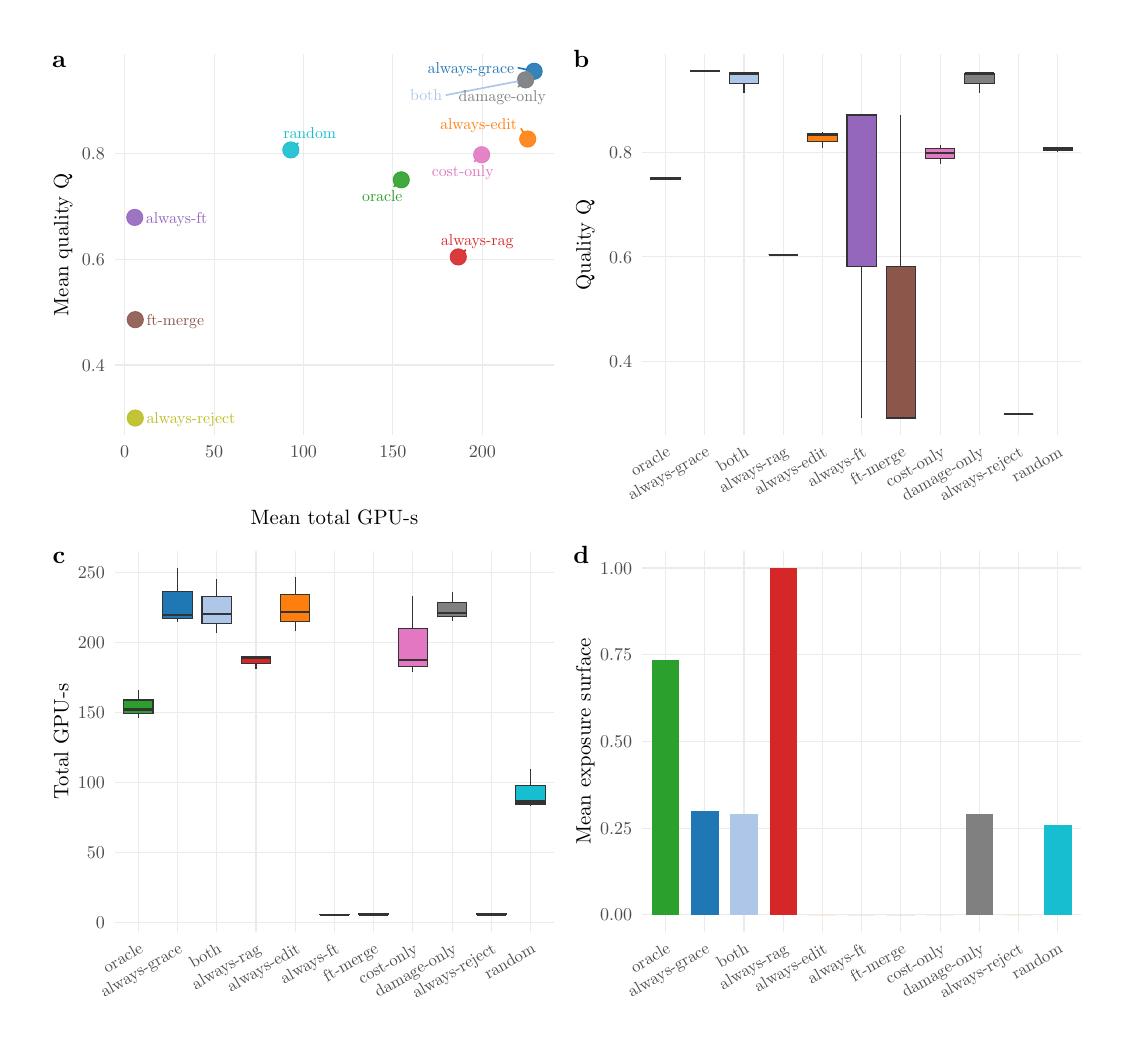
\begin{tikzpicture}[x=1pt,y=1pt]
\definecolor{fillColor}{RGB}{255,255,255}
\path[use as bounding box,fill=fillColor,fill opacity=0.00] (0,0) rectangle (390.26,361.35);
\begin{scope}
\path[clip] (  0.00,  0.00) rectangle (390.26,361.35);
\definecolor{drawColor}{RGB}{255,255,255}
\definecolor{fillColor}{RGB}{255,255,255}

\path[draw=drawColor,line width= 0.6pt,line join=round,line cap=round,fill=fillColor] (  0.00,  0.00) rectangle (390.26,361.35);
\end{scope}
\begin{scope}
\path[clip] (  5.50,176.36) rectangle (194.23,355.85);
\definecolor{fillColor}{RGB}{255,255,255}

\path[fill=fillColor] (  5.50,176.36) rectangle (194.23,355.85);
\end{scope}
\begin{scope}
\path[clip] (194.23,176.36) rectangle (384.76,355.85);
\definecolor{fillColor}{RGB}{255,255,255}

\path[fill=fillColor] (194.23,176.36) rectangle (384.76,355.85);
\end{scope}
\begin{scope}
\path[clip] (  5.50,  5.50) rectangle (194.23,176.36);
\definecolor{fillColor}{RGB}{255,255,255}

\path[fill=fillColor] (  5.50,  5.50) rectangle (194.23,176.36);
\end{scope}
\begin{scope}
\path[clip] (194.23,  5.50) rectangle (384.76,176.36);
\definecolor{fillColor}{RGB}{255,255,255}

\path[fill=fillColor] (194.23,  5.50) rectangle (384.76,176.36);
\end{scope}
\begin{scope}
\path[clip] ( 31.47,214.03) rectangle (190.23,351.85);
\definecolor{drawColor}{gray}{0.92}

\path[draw=drawColor,line width= 0.4pt,line join=round] ( 31.47,239.44) --
	(190.23,239.44);

\path[draw=drawColor,line width= 0.4pt,line join=round] ( 31.47,277.73) --
	(190.23,277.73);

\path[draw=drawColor,line width= 0.4pt,line join=round] ( 31.47,316.02) --
	(190.23,316.02);

\path[draw=drawColor,line width= 0.4pt,line join=round] ( 35.07,214.03) --
	( 35.07,351.85);

\path[draw=drawColor,line width= 0.4pt,line join=round] ( 67.37,214.03) --
	( 67.37,351.85);

\path[draw=drawColor,line width= 0.4pt,line join=round] ( 99.67,214.03) --
	( 99.67,351.85);

\path[draw=drawColor,line width= 0.4pt,line join=round] (131.97,214.03) --
	(131.97,351.85);

\path[draw=drawColor,line width= 0.4pt,line join=round] (164.27,214.03) --
	(164.27,351.85);
\definecolor{drawColor}{RGB}{44,160,44}
\definecolor{fillColor}{RGB}{44,160,44}

\path[draw=drawColor,draw opacity=0.90,line width= 0.3pt,line join=round,line cap=round,fill=fillColor,fill opacity=0.90] (135.00,306.37) circle (  2.94);
\definecolor{drawColor}{RGB}{31,119,180}
\definecolor{fillColor}{RGB}{31,119,180}

\path[draw=drawColor,draw opacity=0.90,line width= 0.3pt,line join=round,line cap=round,fill=fillColor,fill opacity=0.90] (183.01,345.59) circle (  2.94);
\definecolor{drawColor}{RGB}{174,199,232}
\definecolor{fillColor}{RGB}{174,199,232}

\path[draw=drawColor,draw opacity=0.90,line width= 0.3pt,line join=round,line cap=round,fill=fillColor,fill opacity=0.90] (179.82,342.50) circle (  2.94);
\definecolor{drawColor}{RGB}{214,39,40}
\definecolor{fillColor}{RGB}{214,39,40}

\path[draw=drawColor,draw opacity=0.90,line width= 0.3pt,line join=round,line cap=round,fill=fillColor,fill opacity=0.90] (155.60,278.50) circle (  2.94);
\definecolor{drawColor}{RGB}{255,127,14}
\definecolor{fillColor}{RGB}{255,127,14}

\path[draw=drawColor,draw opacity=0.90,line width= 0.3pt,line join=round,line cap=round,fill=fillColor,fill opacity=0.90] (180.69,321.11) circle (  2.94);
\definecolor{drawColor}{RGB}{148,103,189}
\definecolor{fillColor}{RGB}{148,103,189}

\path[draw=drawColor,draw opacity=0.90,line width= 0.3pt,line join=round,line cap=round,fill=fillColor,fill opacity=0.90] ( 38.69,292.78) circle (  2.94);
\definecolor{drawColor}{RGB}{140,86,75}
\definecolor{fillColor}{RGB}{140,86,75}

\path[draw=drawColor,draw opacity=0.90,line width= 0.3pt,line join=round,line cap=round,fill=fillColor,fill opacity=0.90] ( 38.88,255.84) circle (  2.94);
\definecolor{drawColor}{RGB}{227,119,194}
\definecolor{fillColor}{RGB}{227,119,194}

\path[draw=drawColor,draw opacity=0.90,line width= 0.3pt,line join=round,line cap=round,fill=fillColor,fill opacity=0.90] (164.05,315.42) circle (  2.94);
\definecolor{drawColor}{RGB}{127,127,127}
\definecolor{fillColor}{RGB}{127,127,127}

\path[draw=drawColor,draw opacity=0.90,line width= 0.3pt,line join=round,line cap=round,fill=fillColor,fill opacity=0.90] (179.96,342.50) circle (  2.94);
\definecolor{drawColor}{RGB}{188,189,34}
\definecolor{fillColor}{RGB}{188,189,34}

\path[draw=drawColor,draw opacity=0.90,line width= 0.3pt,line join=round,line cap=round,fill=fillColor,fill opacity=0.90] ( 38.88,220.29) circle (  2.94);
\definecolor{drawColor}{RGB}{23,190,207}
\definecolor{fillColor}{RGB}{23,190,207}

\path[draw=drawColor,draw opacity=0.90,line width= 0.3pt,line join=round,line cap=round,fill=fillColor,fill opacity=0.90] ( 95.08,317.16) circle (  2.94);
\definecolor{drawColor}{RGB}{44,160,44}

\path[draw=drawColor,line width= 0.6pt,line join=round,line cap=round] (132.37,303.91) -- (132.90,304.40);
\definecolor{drawColor}{RGB}{31,119,180}

\path[draw=drawColor,line width= 0.6pt,line join=round,line cap=round] (177.24,346.84) -- (180.20,346.20);
\definecolor{drawColor}{RGB}{174,199,232}

\path[draw=drawColor,line width= 0.6pt,line join=round,line cap=round] (151.25,337.00) -- (177.00,341.95);
\definecolor{drawColor}{RGB}{214,39,40}

\path[draw=drawColor,line width= 0.6pt,line join=round,line cap=round] (158.23,280.98) -- (157.69,280.47);
\definecolor{drawColor}{RGB}{255,127,14}

\path[draw=drawColor,line width= 0.6pt,line join=round,line cap=round] (178.29,324.83) -- (179.13,323.53);
\definecolor{drawColor}{RGB}{227,119,194}

\path[draw=drawColor,line width= 0.6pt,line join=round,line cap=round] (161.42,312.95) -- (161.95,313.45);
\definecolor{drawColor}{gray}{0.50}

\path[draw=drawColor,line width= 0.6pt,line join=round,line cap=round] (177.24,340.00) -- (177.84,340.55);
\definecolor{drawColor}{RGB}{23,190,207}

\path[draw=drawColor,line width= 0.6pt,line join=round,line cap=round] ( 97.72,319.64) -- ( 97.18,319.13);
\definecolor{drawColor}{RGB}{44,160,44}

\node[text=drawColor,anchor=base,inner sep=0pt, outer sep=0pt, scale=  0.57] at (128.15,298.48) {oracle};
\definecolor{drawColor}{RGB}{31,119,180}

\node[text=drawColor,anchor=base,inner sep=0pt, outer sep=0pt, scale=  0.57] at (160.14,344.92) {always-grace};
\definecolor{drawColor}{RGB}{174,199,232}

\node[text=drawColor,anchor=base,inner sep=0pt, outer sep=0pt, scale=  0.57] at (143.98,334.97) {both};
\definecolor{drawColor}{RGB}{214,39,40}

\node[text=drawColor,anchor=base,inner sep=0pt, outer sep=0pt, scale=  0.57] at (162.44,282.48) {always-rag};
\definecolor{drawColor}{RGB}{255,127,14}

\node[text=drawColor,anchor=base,inner sep=0pt, outer sep=0pt, scale=  0.57] at (162.94,324.62) {always-edit};
\definecolor{drawColor}{RGB}{148,103,189}

\node[text=drawColor,anchor=base,inner sep=0pt, outer sep=0pt, scale=  0.57] at ( 53.83,290.73) {always-ft};
\definecolor{drawColor}{RGB}{140,86,75}

\node[text=drawColor,anchor=base,inner sep=0pt, outer sep=0pt, scale=  0.57] at ( 53.37,253.91) {ft-merge};
\definecolor{drawColor}{RGB}{227,119,194}

\node[text=drawColor,anchor=base,inner sep=0pt, outer sep=0pt, scale=  0.57] at (157.22,307.53) {cost-only};
\definecolor{drawColor}{gray}{0.50}

\node[text=drawColor,anchor=base,inner sep=0pt, outer sep=0pt, scale=  0.57] at (171.49,334.58) {damage-only};
\definecolor{drawColor}{RGB}{188,189,34}

\node[text=drawColor,anchor=base,inner sep=0pt, outer sep=0pt, scale=  0.57] at ( 58.97,218.16) {always-reject};
\definecolor{drawColor}{RGB}{23,190,207}

\node[text=drawColor,anchor=base,inner sep=0pt, outer sep=0pt, scale=  0.57] at (101.92,321.14) {random};
\end{scope}
\begin{scope}
\path[clip] (  0.00,  0.00) rectangle (390.26,361.35);
\definecolor{drawColor}{gray}{0.30}

\node[text=drawColor,anchor=base east,inner sep=0pt, outer sep=0pt, scale=  0.65] at ( 27.87,237.20) {0.4};

\node[text=drawColor,anchor=base east,inner sep=0pt, outer sep=0pt, scale=  0.65] at ( 27.87,275.49) {0.6};

\node[text=drawColor,anchor=base east,inner sep=0pt, outer sep=0pt, scale=  0.65] at ( 27.87,313.79) {0.8};
\end{scope}
\begin{scope}
\path[clip] (  0.00,  0.00) rectangle (390.26,361.35);
\definecolor{drawColor}{gray}{0.30}

\node[text=drawColor,anchor=base,inner sep=0pt, outer sep=0pt, scale=  0.65] at ( 35.07,205.95) {0};

\node[text=drawColor,anchor=base,inner sep=0pt, outer sep=0pt, scale=  0.65] at ( 67.37,205.95) {50};

\node[text=drawColor,anchor=base,inner sep=0pt, outer sep=0pt, scale=  0.65] at ( 99.67,205.95) {100};

\node[text=drawColor,anchor=base,inner sep=0pt, outer sep=0pt, scale=  0.65] at (131.97,205.95) {150};

\node[text=drawColor,anchor=base,inner sep=0pt, outer sep=0pt, scale=  0.65] at (164.27,205.95) {200};
\end{scope}
\begin{scope}
\path[clip] (  0.00,  0.00) rectangle (390.26,361.35);
\definecolor{drawColor}{RGB}{0,0,0}

\node[text=drawColor,anchor=base,inner sep=0pt, outer sep=0pt, scale=  0.75] at (110.85,181.82) {Mean total GPU-s};
\end{scope}
\begin{scope}
\path[clip] (  0.00,  0.00) rectangle (390.26,361.35);
\definecolor{drawColor}{RGB}{0,0,0}

\node[text=drawColor,rotate= 90.00,anchor=base,inner sep=0pt, outer sep=0pt, scale=  0.75] at ( 14.67,282.94) {Mean quality Q};
\end{scope}
\begin{scope}
\path[clip] (  0.00,  0.00) rectangle (390.26,361.35);
\definecolor{drawColor}{RGB}{0,0,0}

\node[text=drawColor,anchor=base,inner sep=0pt, outer sep=0pt, scale=  0.90] at ( 11.31,347.03) {\bfseries a};
\end{scope}
\begin{scope}
\path[clip] (222.00,214.03) rectangle (380.76,351.85);
\definecolor{drawColor}{gray}{0.92}

\path[draw=drawColor,line width= 0.4pt,line join=round] (222.00,240.64) --
	(380.76,240.64);

\path[draw=drawColor,line width= 0.4pt,line join=round] (222.00,278.50) --
	(380.76,278.50);

\path[draw=drawColor,line width= 0.4pt,line join=round] (222.00,316.36) --
	(380.76,316.36);

\path[draw=drawColor,line width= 0.4pt,line join=round] (230.51,214.03) --
	(230.51,351.85);

\path[draw=drawColor,line width= 0.4pt,line join=round] (244.68,214.03) --
	(244.68,351.85);

\path[draw=drawColor,line width= 0.4pt,line join=round] (258.86,214.03) --
	(258.86,351.85);

\path[draw=drawColor,line width= 0.4pt,line join=round] (273.03,214.03) --
	(273.03,351.85);

\path[draw=drawColor,line width= 0.4pt,line join=round] (287.21,214.03) --
	(287.21,351.85);

\path[draw=drawColor,line width= 0.4pt,line join=round] (301.38,214.03) --
	(301.38,351.85);

\path[draw=drawColor,line width= 0.4pt,line join=round] (315.55,214.03) --
	(315.55,351.85);

\path[draw=drawColor,line width= 0.4pt,line join=round] (329.73,214.03) --
	(329.73,351.85);

\path[draw=drawColor,line width= 0.4pt,line join=round] (343.90,214.03) --
	(343.90,351.85);

\path[draw=drawColor,line width= 0.4pt,line join=round] (358.08,214.03) --
	(358.08,351.85);

\path[draw=drawColor,line width= 0.4pt,line join=round] (372.25,214.03) --
	(372.25,351.85);
\definecolor{drawColor}{gray}{0.20}

\path[draw=drawColor,line width= 0.4pt,line join=round] (230.51,307.04) -- (230.51,307.27);

\path[draw=drawColor,line width= 0.4pt,line join=round] (230.51,306.59) -- (230.51,306.36);
\definecolor{fillColor}{RGB}{44,160,44}

\path[draw=drawColor,line width= 0.4pt,fill=fillColor] (225.19,307.04) --
	(225.19,306.59) --
	(235.82,306.59) --
	(235.82,307.04) --
	(225.19,307.04) --
	cycle;

\path[draw=drawColor,line width= 0.8pt] (225.19,306.82) -- (235.82,306.82);

\path[draw=drawColor,line width= 0.4pt,line join=round] (244.68,345.59) -- (244.68,345.59);

\path[draw=drawColor,line width= 0.4pt,line join=round] (244.68,345.59) -- (244.68,345.59);
\definecolor{fillColor}{RGB}{31,119,180}

\path[draw=drawColor,line width= 0.4pt,fill=fillColor] (239.37,345.59) --
	(239.37,345.59) --
	(250.00,345.59) --
	(250.00,345.59) --
	(239.37,345.59) --
	cycle;

\path[draw=drawColor,line width= 0.8pt] (239.37,345.59) -- (250.00,345.59);

\path[draw=drawColor,line width= 0.4pt,line join=round] (258.86,344.89) -- (258.86,345.00);

\path[draw=drawColor,line width= 0.4pt,line join=round] (258.86,341.30) -- (258.86,337.82);
\definecolor{fillColor}{RGB}{174,199,232}

\path[draw=drawColor,line width= 0.4pt,fill=fillColor] (253.54,344.89) --
	(253.54,341.30) --
	(264.17,341.30) --
	(264.17,344.89) --
	(253.54,344.89) --
	cycle;

\path[draw=drawColor,line width= 0.8pt] (253.54,344.78) -- (264.17,344.78);

\path[draw=drawColor,line width= 0.4pt,line join=round] (273.03,279.26) -- (273.03,279.26);

\path[draw=drawColor,line width= 0.4pt,line join=round] (273.03,279.26) -- (273.03,279.26);
\definecolor{fillColor}{RGB}{214,39,40}

\path[draw=drawColor,line width= 0.4pt,fill=fillColor] (267.72,279.26) --
	(267.72,279.26) --
	(278.35,279.26) --
	(278.35,279.26) --
	(267.72,279.26) --
	cycle;

\path[draw=drawColor,line width= 0.8pt] (267.72,279.26) -- (278.35,279.26);

\path[draw=drawColor,line width= 0.4pt,line join=round] (287.21,323.22) -- (287.21,323.82);

\path[draw=drawColor,line width= 0.4pt,line join=round] (287.21,320.17) -- (287.21,317.73);
\definecolor{fillColor}{RGB}{255,127,14}

\path[draw=drawColor,line width= 0.4pt,fill=fillColor] (281.89,323.22) --
	(281.89,320.17) --
	(292.52,320.17) --
	(292.52,323.22) --
	(281.89,323.22) --
	cycle;

\path[draw=drawColor,line width= 0.8pt] (281.89,322.61) -- (292.52,322.61);

\path[draw=drawColor,line width= 0.4pt,line join=round] (301.38,329.91) -- (301.38,329.91);

\path[draw=drawColor,line width= 0.4pt,line join=round] (301.38,275.10) -- (301.38,220.29);
\definecolor{fillColor}{RGB}{148,103,189}

\path[draw=drawColor,line width= 0.4pt,fill=fillColor] (296.06,329.91) --
	(296.06,275.10) --
	(306.70,275.10) --
	(306.70,329.91) --
	(296.06,329.91) --
	cycle;

\path[draw=drawColor,line width= 0.8pt] (296.06,329.91) -- (306.70,329.91);

\path[draw=drawColor,line width= 0.4pt,line join=round] (315.55,275.13) -- (315.55,329.91);

\path[draw=drawColor,line width= 0.4pt,line join=round] (315.55,220.32) -- (315.55,220.29);
\definecolor{fillColor}{RGB}{140,86,75}

\path[draw=drawColor,line width= 0.4pt,fill=fillColor] (310.24,275.13) --
	(310.24,220.32) --
	(320.87,220.32) --
	(320.87,275.13) --
	(310.24,275.13) --
	cycle;

\path[draw=drawColor,line width= 0.8pt] (310.24,220.34) -- (320.87,220.34);

\path[draw=drawColor,line width= 0.4pt,line join=round] (329.73,317.66) -- (329.73,319.12);

\path[draw=drawColor,line width= 0.4pt,line join=round] (329.73,314.09) -- (329.73,311.97);
\definecolor{fillColor}{RGB}{227,119,194}

\path[draw=drawColor,line width= 0.4pt,fill=fillColor] (324.41,317.66) --
	(324.41,314.09) --
	(335.04,314.09) --
	(335.04,317.66) --
	(324.41,317.66) --
	cycle;

\path[draw=drawColor,line width= 0.8pt] (324.41,316.20) -- (335.04,316.20);

\path[draw=drawColor,line width= 0.4pt,line join=round] (343.90,344.89) -- (343.90,345.00);

\path[draw=drawColor,line width= 0.4pt,line join=round] (343.90,341.30) -- (343.90,337.82);
\definecolor{fillColor}{gray}{0.50}

\path[draw=drawColor,line width= 0.4pt,fill=fillColor] (338.59,344.89) --
	(338.59,341.30) --
	(349.22,341.30) --
	(349.22,344.89) --
	(338.59,344.89) --
	cycle;

\path[draw=drawColor,line width= 0.8pt] (338.59,344.78) -- (349.22,344.78);

\path[draw=drawColor,line width= 0.4pt,line join=round] (358.08,221.71) -- (358.08,221.71);

\path[draw=drawColor,line width= 0.4pt,line join=round] (358.08,221.71) -- (358.08,221.71);
\definecolor{fillColor}{RGB}{188,189,34}

\path[draw=drawColor,line width= 0.4pt,fill=fillColor] (352.76,221.71) --
	(352.76,221.71) --
	(363.39,221.71) --
	(363.39,221.71) --
	(352.76,221.71) --
	cycle;

\path[draw=drawColor,line width= 0.8pt] (352.76,221.71) -- (363.39,221.71);

\path[draw=drawColor,line width= 0.4pt,line join=round] (372.25,318.06) -- (372.25,318.18);

\path[draw=drawColor,line width= 0.4pt,line join=round] (372.25,317.13) -- (372.25,316.32);
\definecolor{fillColor}{RGB}{23,190,207}

\path[draw=drawColor,line width= 0.4pt,fill=fillColor] (366.94,318.06) --
	(366.94,317.13) --
	(377.57,317.13) --
	(377.57,318.06) --
	(366.94,318.06) --
	cycle;

\path[draw=drawColor,line width= 0.8pt] (366.94,317.93) -- (377.57,317.93);
\end{scope}
\begin{scope}
\path[clip] (  0.00,  0.00) rectangle (390.26,361.35);
\definecolor{drawColor}{gray}{0.30}

\node[text=drawColor,anchor=base east,inner sep=0pt, outer sep=0pt, scale=  0.65] at (218.40,238.40) {0.4};

\node[text=drawColor,anchor=base east,inner sep=0pt, outer sep=0pt, scale=  0.65] at (218.40,276.26) {0.6};

\node[text=drawColor,anchor=base east,inner sep=0pt, outer sep=0pt, scale=  0.65] at (218.40,314.12) {0.8};
\end{scope}
\begin{scope}
\path[clip] (  0.00,  0.00) rectangle (390.26,361.35);
\definecolor{drawColor}{gray}{0.30}

\node[text=drawColor,rotate= 30.00,anchor=base east,inner sep=0pt, outer sep=0pt, scale=  0.60] at (232.57,206.85) {oracle};

\node[text=drawColor,rotate= 30.00,anchor=base east,inner sep=0pt, outer sep=0pt, scale=  0.60] at (246.75,206.85) {always-grace};

\node[text=drawColor,rotate= 30.00,anchor=base east,inner sep=0pt, outer sep=0pt, scale=  0.60] at (260.92,206.85) {both};

\node[text=drawColor,rotate= 30.00,anchor=base east,inner sep=0pt, outer sep=0pt, scale=  0.60] at (275.10,206.85) {always-rag};

\node[text=drawColor,rotate= 30.00,anchor=base east,inner sep=0pt, outer sep=0pt, scale=  0.60] at (289.27,206.85) {always-edit};

\node[text=drawColor,rotate= 30.00,anchor=base east,inner sep=0pt, outer sep=0pt, scale=  0.60] at (303.45,206.85) {always-ft};

\node[text=drawColor,rotate= 30.00,anchor=base east,inner sep=0pt, outer sep=0pt, scale=  0.60] at (317.62,206.85) {ft-merge};

\node[text=drawColor,rotate= 30.00,anchor=base east,inner sep=0pt, outer sep=0pt, scale=  0.60] at (331.80,206.85) {cost-only};

\node[text=drawColor,rotate= 30.00,anchor=base east,inner sep=0pt, outer sep=0pt, scale=  0.60] at (345.97,206.85) {damage-only};

\node[text=drawColor,rotate= 30.00,anchor=base east,inner sep=0pt, outer sep=0pt, scale=  0.60] at (360.14,206.85) {always-reject};

\node[text=drawColor,rotate= 30.00,anchor=base east,inner sep=0pt, outer sep=0pt, scale=  0.60] at (374.32,206.85) {random};
\end{scope}
\begin{scope}
\path[clip] (  0.00,  0.00) rectangle (390.26,361.35);
\definecolor{drawColor}{RGB}{0,0,0}

\node[text=drawColor,rotate= 90.00,anchor=base,inner sep=0pt, outer sep=0pt, scale=  0.75] at (203.39,282.94) {Quality Q};
\end{scope}
\begin{scope}
\path[clip] (  0.00,  0.00) rectangle (390.26,361.35);
\definecolor{drawColor}{RGB}{0,0,0}

\node[text=drawColor,anchor=base,inner sep=0pt, outer sep=0pt, scale=  0.90] at (200.05,347.03) {\bfseries b};
\end{scope}
\begin{scope}
\path[clip] ( 31.47, 34.54) rectangle (190.23,172.36);
\definecolor{drawColor}{gray}{0.92}

\path[draw=drawColor,line width= 0.4pt,line join=round] ( 31.47, 38.01) --
	(190.23, 38.01);

\path[draw=drawColor,line width= 0.4pt,line join=round] ( 31.47, 63.31) --
	(190.23, 63.31);

\path[draw=drawColor,line width= 0.4pt,line join=round] ( 31.47, 88.61) --
	(190.23, 88.61);

\path[draw=drawColor,line width= 0.4pt,line join=round] ( 31.47,113.91) --
	(190.23,113.91);

\path[draw=drawColor,line width= 0.4pt,line join=round] ( 31.47,139.21) --
	(190.23,139.21);

\path[draw=drawColor,line width= 0.4pt,line join=round] ( 31.47,164.51) --
	(190.23,164.51);

\path[draw=drawColor,line width= 0.4pt,line join=round] ( 39.98, 34.54) --
	( 39.98,172.36);

\path[draw=drawColor,line width= 0.4pt,line join=round] ( 54.15, 34.54) --
	( 54.15,172.36);

\path[draw=drawColor,line width= 0.4pt,line join=round] ( 68.32, 34.54) --
	( 68.32,172.36);

\path[draw=drawColor,line width= 0.4pt,line join=round] ( 82.50, 34.54) --
	( 82.50,172.36);

\path[draw=drawColor,line width= 0.4pt,line join=round] ( 96.67, 34.54) --
	( 96.67,172.36);

\path[draw=drawColor,line width= 0.4pt,line join=round] (110.85, 34.54) --
	(110.85,172.36);

\path[draw=drawColor,line width= 0.4pt,line join=round] (125.02, 34.54) --
	(125.02,172.36);

\path[draw=drawColor,line width= 0.4pt,line join=round] (139.20, 34.54) --
	(139.20,172.36);

\path[draw=drawColor,line width= 0.4pt,line join=round] (153.37, 34.54) --
	(153.37,172.36);

\path[draw=drawColor,line width= 0.4pt,line join=round] (167.55, 34.54) --
	(167.55,172.36);

\path[draw=drawColor,line width= 0.4pt,line join=round] (181.72, 34.54) --
	(181.72,172.36);
\definecolor{drawColor}{gray}{0.20}

\path[draw=drawColor,line width= 0.4pt,line join=round] ( 39.98,118.41) -- ( 39.98,121.84);

\path[draw=drawColor,line width= 0.4pt,line join=round] ( 39.98,113.50) -- ( 39.98,112.03);
\definecolor{fillColor}{RGB}{44,160,44}

\path[draw=drawColor,line width= 0.4pt,fill=fillColor] ( 34.66,118.41) --
	( 34.66,113.50) --
	( 45.29,113.50) --
	( 45.29,118.41) --
	( 34.66,118.41) --
	cycle;

\path[draw=drawColor,line width= 0.8pt] ( 34.66,114.97) -- ( 45.29,114.97);

\path[draw=drawColor,line width= 0.4pt,line join=round] ( 54.15,157.56) -- ( 54.15,166.10);

\path[draw=drawColor,line width= 0.4pt,line join=round] ( 54.15,147.78) -- ( 54.15,146.55);
\definecolor{fillColor}{RGB}{31,119,180}

\path[draw=drawColor,line width= 0.4pt,fill=fillColor] ( 48.83,157.56) --
	( 48.83,147.78) --
	( 59.47,147.78) --
	( 59.47,157.56) --
	( 48.83,157.56) --
	cycle;

\path[draw=drawColor,line width= 0.8pt] ( 48.83,149.01) -- ( 59.47,149.01);

\path[draw=drawColor,line width= 0.4pt,line join=round] ( 68.32,155.84) -- ( 68.32,162.11);

\path[draw=drawColor,line width= 0.4pt,line join=round] ( 68.32,146.03) -- ( 68.32,142.49);
\definecolor{fillColor}{RGB}{174,199,232}

\path[draw=drawColor,line width= 0.4pt,fill=fillColor] ( 63.01,155.84) --
	( 63.01,146.03) --
	( 73.64,146.03) --
	( 73.64,155.84) --
	( 63.01,155.84) --
	cycle;

\path[draw=drawColor,line width= 0.8pt] ( 63.01,149.57) -- ( 73.64,149.57);

\path[draw=drawColor,line width= 0.4pt,line join=round] ( 82.50,133.85) -- ( 82.50,133.94);

\path[draw=drawColor,line width= 0.4pt,line join=round] ( 82.50,131.65) -- ( 82.50,129.54);
\definecolor{fillColor}{RGB}{214,39,40}

\path[draw=drawColor,line width= 0.4pt,fill=fillColor] ( 77.18,133.85) --
	( 77.18,131.65) --
	( 87.81,131.65) --
	( 87.81,133.85) --
	( 77.18,133.85) --
	cycle;

\path[draw=drawColor,line width= 0.8pt] ( 77.18,133.77) -- ( 87.81,133.77);

\path[draw=drawColor,line width= 0.4pt,line join=round] ( 96.67,156.49) -- ( 96.67,162.72);

\path[draw=drawColor,line width= 0.4pt,line join=round] ( 96.67,146.75) -- ( 96.67,143.25);
\definecolor{fillColor}{RGB}{255,127,14}

\path[draw=drawColor,line width= 0.4pt,fill=fillColor] ( 91.36,156.49) --
	( 91.36,146.75) --
	(101.99,146.75) --
	(101.99,156.49) --
	( 91.36,156.49) --
	cycle;

\path[draw=drawColor,line width= 0.8pt] ( 91.36,150.25) -- (101.99,150.25);

\path[draw=drawColor,line width= 0.4pt,line join=round] (110.85, 40.86) -- (110.85, 40.90);

\path[draw=drawColor,line width= 0.4pt,line join=round] (110.85, 40.82) -- (110.85, 40.81);
\definecolor{fillColor}{RGB}{148,103,189}

\path[draw=drawColor,line width= 0.4pt,fill=fillColor] (105.53, 40.86) --
	(105.53, 40.82) --
	(116.16, 40.82) --
	(116.16, 40.86) --
	(105.53, 40.86) --
	cycle;

\path[draw=drawColor,line width= 0.8pt] (105.53, 40.82) -- (116.16, 40.82);

\path[draw=drawColor,line width= 0.4pt,line join=round] (125.02, 41.09) -- (125.02, 41.31);

\path[draw=drawColor,line width= 0.4pt,line join=round] (125.02, 40.84) -- (125.02, 40.81);
\definecolor{fillColor}{RGB}{140,86,75}

\path[draw=drawColor,line width= 0.4pt,fill=fillColor] (119.71, 41.09) --
	(119.71, 40.84) --
	(130.34, 40.84) --
	(130.34, 41.09) --
	(119.71, 41.09) --
	cycle;

\path[draw=drawColor,line width= 0.8pt] (119.71, 40.87) -- (130.34, 40.87);

\path[draw=drawColor,line width= 0.4pt,line join=round] (139.20,144.39) -- (139.20,156.01);

\path[draw=drawColor,line width= 0.4pt,line join=round] (139.20,130.55) -- (139.20,128.34);
\definecolor{fillColor}{RGB}{227,119,194}

\path[draw=drawColor,line width= 0.4pt,fill=fillColor] (133.88,144.39) --
	(133.88,130.55) --
	(144.51,130.55) --
	(144.51,144.39) --
	(133.88,144.39) --
	cycle;

\path[draw=drawColor,line width= 0.8pt] (133.88,132.76) -- (144.51,132.76);

\path[draw=drawColor,line width= 0.4pt,line join=round] (153.37,153.70) -- (153.37,157.50);

\path[draw=drawColor,line width= 0.4pt,line join=round] (153.37,148.50) -- (153.37,147.09);
\definecolor{fillColor}{gray}{0.50}

\path[draw=drawColor,line width= 0.4pt,fill=fillColor] (148.06,153.70) --
	(148.06,148.50) --
	(158.69,148.50) --
	(158.69,153.70) --
	(148.06,153.70) --
	cycle;

\path[draw=drawColor,line width= 0.8pt] (148.06,149.91) -- (158.69,149.91);

\path[draw=drawColor,line width= 0.4pt,line join=round] (167.55, 41.09) -- (167.55, 41.35);

\path[draw=drawColor,line width= 0.4pt,line join=round] (167.55, 40.82) -- (167.55, 40.81);
\definecolor{fillColor}{RGB}{188,189,34}

\path[draw=drawColor,line width= 0.4pt,fill=fillColor] (162.23, 41.09) --
	(162.23, 40.82) --
	(172.86, 40.82) --
	(172.86, 41.09) --
	(162.23, 41.09) --
	cycle;

\path[draw=drawColor,line width= 0.8pt] (162.23, 40.82) -- (172.86, 40.82);

\path[draw=drawColor,line width= 0.4pt,line join=round] (181.72, 87.55) -- (181.72, 93.36);

\path[draw=drawColor,line width= 0.4pt,line join=round] (181.72, 80.84) -- (181.72, 79.95);
\definecolor{fillColor}{RGB}{23,190,207}

\path[draw=drawColor,line width= 0.4pt,fill=fillColor] (176.41, 87.55) --
	(176.41, 80.84) --
	(187.04, 80.84) --
	(187.04, 87.55) --
	(176.41, 87.55) --
	cycle;

\path[draw=drawColor,line width= 0.8pt] (176.41, 81.73) -- (187.04, 81.73);
\end{scope}
\begin{scope}
\path[clip] (  0.00,  0.00) rectangle (390.26,361.35);
\definecolor{drawColor}{gray}{0.30}

\node[text=drawColor,anchor=base east,inner sep=0pt, outer sep=0pt, scale=  0.65] at ( 27.87, 35.77) {0};

\node[text=drawColor,anchor=base east,inner sep=0pt, outer sep=0pt, scale=  0.65] at ( 27.87, 61.07) {50};

\node[text=drawColor,anchor=base east,inner sep=0pt, outer sep=0pt, scale=  0.65] at ( 27.87, 86.37) {100};

\node[text=drawColor,anchor=base east,inner sep=0pt, outer sep=0pt, scale=  0.65] at ( 27.87,111.67) {150};

\node[text=drawColor,anchor=base east,inner sep=0pt, outer sep=0pt, scale=  0.65] at ( 27.87,136.97) {200};

\node[text=drawColor,anchor=base east,inner sep=0pt, outer sep=0pt, scale=  0.65] at ( 27.87,162.27) {250};
\end{scope}
\begin{scope}
\path[clip] (  0.00,  0.00) rectangle (390.26,361.35);
\definecolor{drawColor}{gray}{0.30}

\node[text=drawColor,rotate= 30.00,anchor=base east,inner sep=0pt, outer sep=0pt, scale=  0.60] at ( 42.04, 27.36) {oracle};

\node[text=drawColor,rotate= 30.00,anchor=base east,inner sep=0pt, outer sep=0pt, scale=  0.60] at ( 56.22, 27.36) {always-grace};

\node[text=drawColor,rotate= 30.00,anchor=base east,inner sep=0pt, outer sep=0pt, scale=  0.60] at ( 70.39, 27.36) {both};

\node[text=drawColor,rotate= 30.00,anchor=base east,inner sep=0pt, outer sep=0pt, scale=  0.60] at ( 84.57, 27.36) {always-rag};

\node[text=drawColor,rotate= 30.00,anchor=base east,inner sep=0pt, outer sep=0pt, scale=  0.60] at ( 98.74, 27.36) {always-edit};

\node[text=drawColor,rotate= 30.00,anchor=base east,inner sep=0pt, outer sep=0pt, scale=  0.60] at (112.91, 27.36) {always-ft};

\node[text=drawColor,rotate= 30.00,anchor=base east,inner sep=0pt, outer sep=0pt, scale=  0.60] at (127.09, 27.36) {ft-merge};

\node[text=drawColor,rotate= 30.00,anchor=base east,inner sep=0pt, outer sep=0pt, scale=  0.60] at (141.26, 27.36) {cost-only};

\node[text=drawColor,rotate= 30.00,anchor=base east,inner sep=0pt, outer sep=0pt, scale=  0.60] at (155.44, 27.36) {damage-only};

\node[text=drawColor,rotate= 30.00,anchor=base east,inner sep=0pt, outer sep=0pt, scale=  0.60] at (169.61, 27.36) {always-reject};

\node[text=drawColor,rotate= 30.00,anchor=base east,inner sep=0pt, outer sep=0pt, scale=  0.60] at (183.79, 27.36) {random};
\end{scope}
\begin{scope}
\path[clip] (  0.00,  0.00) rectangle (390.26,361.35);
\definecolor{drawColor}{RGB}{0,0,0}

\node[text=drawColor,rotate= 90.00,anchor=base,inner sep=0pt, outer sep=0pt, scale=  0.75] at ( 14.67,103.45) {Total GPU-s};
\end{scope}
\begin{scope}
\path[clip] (  0.00,  0.00) rectangle (390.26,361.35);
\definecolor{drawColor}{RGB}{0,0,0}

\node[text=drawColor,anchor=base,inner sep=0pt, outer sep=0pt, scale=  0.90] at ( 11.31,167.63) {\bfseries c};
\end{scope}
\begin{scope}
\path[clip] (222.00, 34.54) rectangle (380.76,172.36);
\definecolor{drawColor}{gray}{0.92}

\path[draw=drawColor,line width= 0.4pt,line join=round] (222.00, 40.81) --
	(380.76, 40.81);

\path[draw=drawColor,line width= 0.4pt,line join=round] (222.00, 72.13) --
	(380.76, 72.13);

\path[draw=drawColor,line width= 0.4pt,line join=round] (222.00,103.45) --
	(380.76,103.45);

\path[draw=drawColor,line width= 0.4pt,line join=round] (222.00,134.78) --
	(380.76,134.78);

\path[draw=drawColor,line width= 0.4pt,line join=round] (222.00,166.10) --
	(380.76,166.10);

\path[draw=drawColor,line width= 0.4pt,line join=round] (230.51, 34.54) --
	(230.51,172.36);

\path[draw=drawColor,line width= 0.4pt,line join=round] (244.68, 34.54) --
	(244.68,172.36);

\path[draw=drawColor,line width= 0.4pt,line join=round] (258.86, 34.54) --
	(258.86,172.36);

\path[draw=drawColor,line width= 0.4pt,line join=round] (273.03, 34.54) --
	(273.03,172.36);

\path[draw=drawColor,line width= 0.4pt,line join=round] (287.21, 34.54) --
	(287.21,172.36);

\path[draw=drawColor,line width= 0.4pt,line join=round] (301.38, 34.54) --
	(301.38,172.36);

\path[draw=drawColor,line width= 0.4pt,line join=round] (315.55, 34.54) --
	(315.55,172.36);

\path[draw=drawColor,line width= 0.4pt,line join=round] (329.73, 34.54) --
	(329.73,172.36);

\path[draw=drawColor,line width= 0.4pt,line join=round] (343.90, 34.54) --
	(343.90,172.36);

\path[draw=drawColor,line width= 0.4pt,line join=round] (358.08, 34.54) --
	(358.08,172.36);

\path[draw=drawColor,line width= 0.4pt,line join=round] (372.25, 34.54) --
	(372.25,172.36);
\definecolor{fillColor}{RGB}{44,160,44}

\path[fill=fillColor] (225.55, 40.81) rectangle (235.47,132.71);
\definecolor{fillColor}{RGB}{31,119,180}

\path[fill=fillColor] (239.72, 40.81) rectangle (249.64, 78.40);
\definecolor{fillColor}{RGB}{174,199,232}

\path[fill=fillColor] (253.90, 40.81) rectangle (263.82, 77.34);
\definecolor{fillColor}{RGB}{214,39,40}

\path[fill=fillColor] (268.07, 40.81) rectangle (277.99,166.10);
\definecolor{fillColor}{RGB}{255,127,14}

\path[fill=fillColor] (282.24, 40.81) rectangle (292.17, 40.81);
\definecolor{fillColor}{RGB}{148,103,189}

\path[fill=fillColor] (296.42, 40.81) rectangle (306.34, 40.81);
\definecolor{fillColor}{RGB}{140,86,75}

\path[fill=fillColor] (310.59, 40.81) rectangle (320.52, 40.81);
\definecolor{fillColor}{RGB}{227,119,194}

\path[fill=fillColor] (324.77, 40.81) rectangle (334.69, 40.81);
\definecolor{fillColor}{gray}{0.50}

\path[fill=fillColor] (338.94, 40.81) rectangle (348.87, 77.34);
\definecolor{fillColor}{RGB}{188,189,34}

\path[fill=fillColor] (353.12, 40.81) rectangle (363.04, 40.81);
\definecolor{fillColor}{RGB}{23,190,207}

\path[fill=fillColor] (367.29, 40.81) rectangle (377.21, 73.09);
\end{scope}
\begin{scope}
\path[clip] (  0.00,  0.00) rectangle (390.26,361.35);
\definecolor{drawColor}{gray}{0.30}

\node[text=drawColor,anchor=base east,inner sep=0pt, outer sep=0pt, scale=  0.65] at (218.40, 38.57) {0.00};

\node[text=drawColor,anchor=base east,inner sep=0pt, outer sep=0pt, scale=  0.65] at (218.40, 69.89) {0.25};

\node[text=drawColor,anchor=base east,inner sep=0pt, outer sep=0pt, scale=  0.65] at (218.40,101.21) {0.50};

\node[text=drawColor,anchor=base east,inner sep=0pt, outer sep=0pt, scale=  0.65] at (218.40,132.54) {0.75};

\node[text=drawColor,anchor=base east,inner sep=0pt, outer sep=0pt, scale=  0.65] at (218.40,163.86) {1.00};
\end{scope}
\begin{scope}
\path[clip] (  0.00,  0.00) rectangle (390.26,361.35);
\definecolor{drawColor}{gray}{0.30}

\node[text=drawColor,rotate= 30.00,anchor=base east,inner sep=0pt, outer sep=0pt, scale=  0.60] at (232.57, 27.36) {oracle};

\node[text=drawColor,rotate= 30.00,anchor=base east,inner sep=0pt, outer sep=0pt, scale=  0.60] at (246.75, 27.36) {always-grace};

\node[text=drawColor,rotate= 30.00,anchor=base east,inner sep=0pt, outer sep=0pt, scale=  0.60] at (260.92, 27.36) {both};

\node[text=drawColor,rotate= 30.00,anchor=base east,inner sep=0pt, outer sep=0pt, scale=  0.60] at (275.10, 27.36) {always-rag};

\node[text=drawColor,rotate= 30.00,anchor=base east,inner sep=0pt, outer sep=0pt, scale=  0.60] at (289.27, 27.36) {always-edit};

\node[text=drawColor,rotate= 30.00,anchor=base east,inner sep=0pt, outer sep=0pt, scale=  0.60] at (303.45, 27.36) {always-ft};

\node[text=drawColor,rotate= 30.00,anchor=base east,inner sep=0pt, outer sep=0pt, scale=  0.60] at (317.62, 27.36) {ft-merge};

\node[text=drawColor,rotate= 30.00,anchor=base east,inner sep=0pt, outer sep=0pt, scale=  0.60] at (331.80, 27.36) {cost-only};

\node[text=drawColor,rotate= 30.00,anchor=base east,inner sep=0pt, outer sep=0pt, scale=  0.60] at (345.97, 27.36) {damage-only};

\node[text=drawColor,rotate= 30.00,anchor=base east,inner sep=0pt, outer sep=0pt, scale=  0.60] at (360.14, 27.36) {always-reject};

\node[text=drawColor,rotate= 30.00,anchor=base east,inner sep=0pt, outer sep=0pt, scale=  0.60] at (374.32, 27.36) {random};
\end{scope}
\begin{scope}
\path[clip] (  0.00,  0.00) rectangle (390.26,361.35);
\definecolor{drawColor}{RGB}{0,0,0}

\node[text=drawColor,rotate= 90.00,anchor=base,inner sep=0pt, outer sep=0pt, scale=  0.75] at (203.39,103.45) {Mean exposure surface};
\end{scope}
\begin{scope}
\path[clip] (  0.00,  0.00) rectangle (390.26,361.35);
\definecolor{drawColor}{RGB}{0,0,0}

\node[text=drawColor,anchor=base,inner sep=0pt, outer sep=0pt, scale=  0.90] at (200.05,167.63) {\bfseries d};
\end{scope}
\end{tikzpicture}

\caption{Router arm-selection counts (ROME vs.\ GRACE vs.\ RAG vs.\ FT) across stream configurations.
Routing-share figure regenerated from canonical measurement artifacts.}
\label{fig:router}
\end{figure}

\subsection{Damage discovery (predictor moat)}
\begin{figure}[t]
\centering
% SOURCE: edit-harness/results/frame_a/cells/cell_*_real_MIX_{A,B,C}_*.json + results/D3_benefit_predictor_eval.json
% !TEX encoding = UTF-8 Unicode
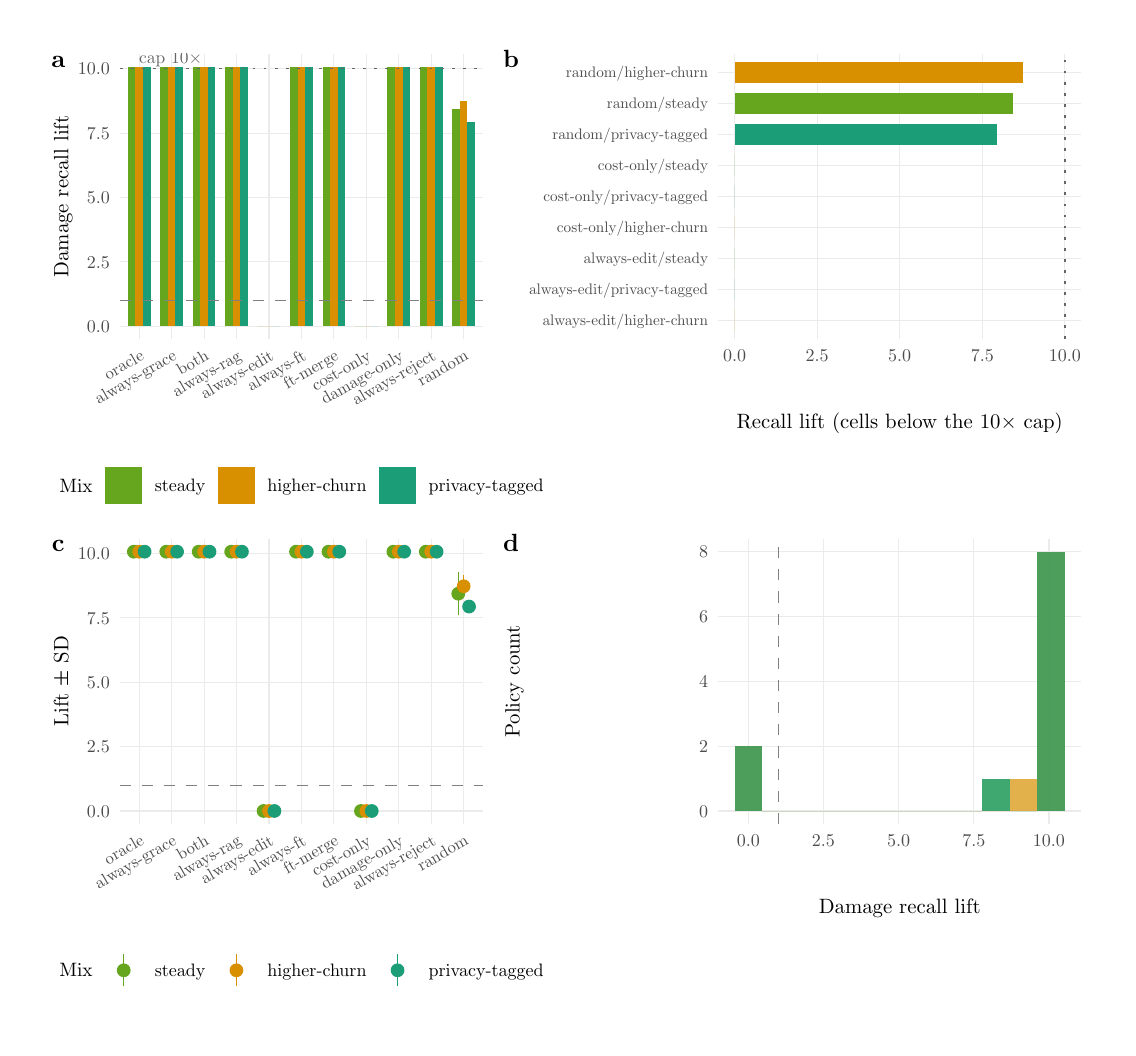
\begin{tikzpicture}[x=1pt,y=1pt]
\definecolor{fillColor}{RGB}{255,255,255}
\path[use as bounding box,fill=fillColor,fill opacity=0.00] (0,0) rectangle (390.26,361.35);
\begin{scope}
\path[clip] (  0.00,  0.00) rectangle (390.26,361.35);
\definecolor{drawColor}{RGB}{255,255,255}
\definecolor{fillColor}{RGB}{255,255,255}

\path[draw=drawColor,line width= 0.6pt,line join=round,line cap=round,fill=fillColor] (  0.00,  0.00) rectangle (390.26,361.35);
\end{scope}
\begin{scope}
\path[clip] (  5.50,180.68) rectangle (168.58,355.85);
\definecolor{fillColor}{RGB}{255,255,255}

\path[fill=fillColor] (  5.50,180.68) rectangle (168.58,355.85);
\end{scope}
\begin{scope}
\path[clip] (168.58,180.68) rectangle (384.76,355.85);
\definecolor{fillColor}{RGB}{255,255,255}

\path[fill=fillColor] (168.58,180.68) rectangle (384.76,355.85);
\end{scope}
\begin{scope}
\path[clip] (  5.50,  5.50) rectangle (168.58,180.67);
\definecolor{fillColor}{RGB}{255,255,255}

\path[fill=fillColor] (  5.50,  5.50) rectangle (168.58,180.67);
\end{scope}
\begin{scope}
\path[clip] (168.58,  5.50) rectangle (384.76,180.67);
\definecolor{fillColor}{RGB}{255,255,255}

\path[fill=fillColor] (168.58,  5.50) rectangle (384.76,180.67);
\end{scope}
\begin{scope}
\path[clip] ( 33.28,248.80) rectangle (164.58,351.85);
\definecolor{drawColor}{gray}{0.92}

\path[draw=drawColor,line width= 0.4pt,line join=round] ( 33.28,253.48) --
	(164.58,253.48);

\path[draw=drawColor,line width= 0.4pt,line join=round] ( 33.28,276.74) --
	(164.58,276.74);

\path[draw=drawColor,line width= 0.4pt,line join=round] ( 33.28,299.99) --
	(164.58,299.99);

\path[draw=drawColor,line width= 0.4pt,line join=round] ( 33.28,323.25) --
	(164.58,323.25);

\path[draw=drawColor,line width= 0.4pt,line join=round] ( 33.28,346.51) --
	(164.58,346.51);

\path[draw=drawColor,line width= 0.4pt,line join=round] ( 40.31,248.80) --
	( 40.31,351.85);

\path[draw=drawColor,line width= 0.4pt,line join=round] ( 52.03,248.80) --
	( 52.03,351.85);

\path[draw=drawColor,line width= 0.4pt,line join=round] ( 63.76,248.80) --
	( 63.76,351.85);

\path[draw=drawColor,line width= 0.4pt,line join=round] ( 75.48,248.80) --
	( 75.48,351.85);

\path[draw=drawColor,line width= 0.4pt,line join=round] ( 87.20,248.80) --
	( 87.20,351.85);

\path[draw=drawColor,line width= 0.4pt,line join=round] ( 98.93,248.80) --
	( 98.93,351.85);

\path[draw=drawColor,line width= 0.4pt,line join=round] (110.65,248.80) --
	(110.65,351.85);

\path[draw=drawColor,line width= 0.4pt,line join=round] (122.37,248.80) --
	(122.37,351.85);

\path[draw=drawColor,line width= 0.4pt,line join=round] (134.10,248.80) --
	(134.10,351.85);

\path[draw=drawColor,line width= 0.4pt,line join=round] (145.82,248.80) --
	(145.82,351.85);

\path[draw=drawColor,line width= 0.4pt,line join=round] (157.54,248.80) --
	(157.54,351.85);
\definecolor{fillColor}{RGB}{102,166,31}

\path[fill=fillColor] ( 36.21,253.48) rectangle ( 38.94,347.17);

\path[fill=fillColor] ( 47.93,253.48) rectangle ( 50.67,347.17);

\path[fill=fillColor] ( 59.65,253.48) rectangle ( 62.39,347.17);

\path[fill=fillColor] ( 71.38,253.48) rectangle ( 74.11,347.17);

\path[fill=fillColor] ( 83.10,253.48) rectangle ( 85.84,253.48);

\path[fill=fillColor] ( 94.82,253.48) rectangle ( 97.56,347.17);

\path[fill=fillColor] (106.55,253.48) rectangle (109.28,347.17);

\path[fill=fillColor] (118.27,253.48) rectangle (121.01,253.48);

\path[fill=fillColor] (129.99,253.48) rectangle (132.73,347.17);

\path[fill=fillColor] (141.72,253.48) rectangle (144.45,347.17);

\path[fill=fillColor] (153.44,253.48) rectangle (156.18,332.00);
\definecolor{fillColor}{RGB}{216,144,0}

\path[fill=fillColor] ( 38.94,253.48) rectangle ( 41.68,347.17);

\path[fill=fillColor] ( 50.67,253.48) rectangle ( 53.40,347.17);

\path[fill=fillColor] ( 62.39,253.48) rectangle ( 65.12,347.17);

\path[fill=fillColor] ( 74.11,253.48) rectangle ( 76.85,347.17);

\path[fill=fillColor] ( 85.84,253.48) rectangle ( 88.57,253.48);

\path[fill=fillColor] ( 97.56,253.48) rectangle (100.29,347.17);

\path[fill=fillColor] (109.28,253.48) rectangle (112.02,347.17);

\path[fill=fillColor] (121.01,253.48) rectangle (123.74,253.48);

\path[fill=fillColor] (132.73,253.48) rectangle (135.46,347.17);

\path[fill=fillColor] (144.45,253.48) rectangle (147.19,347.17);

\path[fill=fillColor] (156.18,253.48) rectangle (158.91,334.67);
\definecolor{fillColor}{RGB}{27,158,119}

\path[fill=fillColor] ( 41.68,253.48) rectangle ( 44.41,347.17);

\path[fill=fillColor] ( 53.40,253.48) rectangle ( 56.14,347.17);

\path[fill=fillColor] ( 65.12,253.48) rectangle ( 67.86,347.17);

\path[fill=fillColor] ( 76.85,253.48) rectangle ( 79.58,347.17);

\path[fill=fillColor] ( 88.57,253.48) rectangle ( 91.31,253.48);

\path[fill=fillColor] (100.29,253.48) rectangle (103.03,347.17);

\path[fill=fillColor] (112.02,253.48) rectangle (114.75,347.17);

\path[fill=fillColor] (123.74,253.48) rectangle (126.48,253.48);

\path[fill=fillColor] (135.46,253.48) rectangle (138.20,347.17);

\path[fill=fillColor] (147.19,253.48) rectangle (149.92,347.17);

\path[fill=fillColor] (158.91,253.48) rectangle (161.65,327.35);
\definecolor{drawColor}{gray}{0.50}

\path[draw=drawColor,line width= 0.5pt,dash pattern=on 4pt off 4pt ,line join=round] ( 33.28,262.78) -- (164.58,262.78);
\definecolor{drawColor}{gray}{0.40}

\path[draw=drawColor,line width= 0.5pt,dash pattern=on 1pt off 3pt ,line join=round] ( 33.28,346.51) -- (164.58,346.51);

\node[text=drawColor,anchor=base west,inner sep=0pt, outer sep=0pt, scale=  0.63] at ( 40.31,348.23) {cap $10\times$};
\end{scope}
\begin{scope}
\path[clip] (  0.00,  0.00) rectangle (390.26,361.35);
\definecolor{drawColor}{gray}{0.30}

\node[text=drawColor,anchor=base east,inner sep=0pt, outer sep=0pt, scale=  0.65] at ( 29.68,251.24) {0.0};

\node[text=drawColor,anchor=base east,inner sep=0pt, outer sep=0pt, scale=  0.65] at ( 29.68,274.50) {2.5};

\node[text=drawColor,anchor=base east,inner sep=0pt, outer sep=0pt, scale=  0.65] at ( 29.68,297.76) {5.0};

\node[text=drawColor,anchor=base east,inner sep=0pt, outer sep=0pt, scale=  0.65] at ( 29.68,321.01) {7.5};

\node[text=drawColor,anchor=base east,inner sep=0pt, outer sep=0pt, scale=  0.65] at ( 29.68,344.27) {10.0};
\end{scope}
\begin{scope}
\path[clip] (  0.00,  0.00) rectangle (390.26,361.35);
\definecolor{drawColor}{gray}{0.30}

\node[text=drawColor,rotate= 30.00,anchor=base east,inner sep=0pt, outer sep=0pt, scale=  0.60] at ( 42.38,241.62) {oracle};

\node[text=drawColor,rotate= 30.00,anchor=base east,inner sep=0pt, outer sep=0pt, scale=  0.60] at ( 54.10,241.62) {always-grace};

\node[text=drawColor,rotate= 30.00,anchor=base east,inner sep=0pt, outer sep=0pt, scale=  0.60] at ( 65.82,241.62) {both};

\node[text=drawColor,rotate= 30.00,anchor=base east,inner sep=0pt, outer sep=0pt, scale=  0.60] at ( 77.55,241.62) {always-rag};

\node[text=drawColor,rotate= 30.00,anchor=base east,inner sep=0pt, outer sep=0pt, scale=  0.60] at ( 89.27,241.62) {always-edit};

\node[text=drawColor,rotate= 30.00,anchor=base east,inner sep=0pt, outer sep=0pt, scale=  0.60] at (100.99,241.62) {always-ft};

\node[text=drawColor,rotate= 30.00,anchor=base east,inner sep=0pt, outer sep=0pt, scale=  0.60] at (112.72,241.62) {ft-merge};

\node[text=drawColor,rotate= 30.00,anchor=base east,inner sep=0pt, outer sep=0pt, scale=  0.60] at (124.44,241.62) {cost-only};

\node[text=drawColor,rotate= 30.00,anchor=base east,inner sep=0pt, outer sep=0pt, scale=  0.60] at (136.16,241.62) {damage-only};

\node[text=drawColor,rotate= 30.00,anchor=base east,inner sep=0pt, outer sep=0pt, scale=  0.60] at (147.89,241.62) {always-reject};

\node[text=drawColor,rotate= 30.00,anchor=base east,inner sep=0pt, outer sep=0pt, scale=  0.60] at (159.61,241.62) {random};
\end{scope}
\begin{scope}
\path[clip] (  0.00,  0.00) rectangle (390.26,361.35);
\definecolor{drawColor}{RGB}{0,0,0}

\node[text=drawColor,rotate= 90.00,anchor=base,inner sep=0pt, outer sep=0pt, scale=  0.75] at ( 14.67,300.32) {Damage recall lift};
\end{scope}
\begin{scope}
\path[clip] (  0.00,  0.00) rectangle (390.26,361.35);
\definecolor{drawColor}{RGB}{0,0,0}

\node[text=drawColor,anchor=base west,inner sep=0pt, outer sep=0pt, scale=  0.70] at ( 11.43,193.49) {Mix};
\end{scope}
\begin{scope}
\path[clip] (  0.00,  0.00) rectangle (390.26,361.35);
\definecolor{fillColor}{RGB}{102,166,31}

\path[fill=fillColor] ( 28.00,189.19) rectangle ( 41.42,202.61);
\end{scope}
\begin{scope}
\path[clip] (  0.00,  0.00) rectangle (390.26,361.35);
\definecolor{fillColor}{RGB}{216,144,0}

\path[fill=fillColor] ( 68.72,189.19) rectangle ( 82.14,202.61);
\end{scope}
\begin{scope}
\path[clip] (  0.00,  0.00) rectangle (390.26,361.35);
\definecolor{fillColor}{RGB}{27,158,119}

\path[fill=fillColor] (126.95,189.19) rectangle (140.37,202.61);
\end{scope}
\begin{scope}
\path[clip] (  0.00,  0.00) rectangle (390.26,361.35);
\definecolor{drawColor}{RGB}{0,0,0}

\node[text=drawColor,anchor=base west,inner sep=0pt, outer sep=0pt, scale=  0.65] at ( 45.94,193.66) {steady};
\end{scope}
\begin{scope}
\path[clip] (  0.00,  0.00) rectangle (390.26,361.35);
\definecolor{drawColor}{RGB}{0,0,0}

\node[text=drawColor,anchor=base west,inner sep=0pt, outer sep=0pt, scale=  0.65] at ( 86.66,193.66) {higher-churn};
\end{scope}
\begin{scope}
\path[clip] (  0.00,  0.00) rectangle (390.26,361.35);
\definecolor{drawColor}{RGB}{0,0,0}

\node[text=drawColor,anchor=base west,inner sep=0pt, outer sep=0pt, scale=  0.65] at (144.89,193.66) {privacy-tagged};
\end{scope}
\begin{scope}
\path[clip] (  0.00,  0.00) rectangle (390.26,361.35);
\definecolor{drawColor}{RGB}{0,0,0}

\node[text=drawColor,anchor=base,inner sep=0pt, outer sep=0pt, scale=  0.90] at ( 11.05,347.07) {\bfseries a};
\end{scope}
\begin{scope}
\path[clip] (249.46,248.80) rectangle (380.76,351.85);
\definecolor{drawColor}{gray}{0.92}

\path[draw=drawColor,line width= 0.4pt,line join=round] (249.46,255.52) --
	(380.76,255.52);

\path[draw=drawColor,line width= 0.4pt,line join=round] (249.46,266.72) --
	(380.76,266.72);

\path[draw=drawColor,line width= 0.4pt,line join=round] (249.46,277.92) --
	(380.76,277.92);

\path[draw=drawColor,line width= 0.4pt,line join=round] (249.46,289.12) --
	(380.76,289.12);

\path[draw=drawColor,line width= 0.4pt,line join=round] (249.46,300.32) --
	(380.76,300.32);

\path[draw=drawColor,line width= 0.4pt,line join=round] (249.46,311.52) --
	(380.76,311.52);

\path[draw=drawColor,line width= 0.4pt,line join=round] (249.46,322.73) --
	(380.76,322.73);

\path[draw=drawColor,line width= 0.4pt,line join=round] (249.46,333.93) --
	(380.76,333.93);

\path[draw=drawColor,line width= 0.4pt,line join=round] (249.46,345.13) --
	(380.76,345.13);

\path[draw=drawColor,line width= 0.4pt,line join=round] (255.42,248.80) --
	(255.42,351.85);

\path[draw=drawColor,line width= 0.4pt,line join=round] (285.27,248.80) --
	(285.27,351.85);

\path[draw=drawColor,line width= 0.4pt,line join=round] (315.11,248.80) --
	(315.11,351.85);

\path[draw=drawColor,line width= 0.4pt,line join=round] (344.95,248.80) --
	(344.95,351.85);

\path[draw=drawColor,line width= 0.4pt,line join=round] (374.79,248.80) --
	(374.79,351.85);
\definecolor{fillColor}{RGB}{102,166,31}

\path[fill=fillColor] (255.42,274.00) rectangle (255.42,281.84);

\path[fill=fillColor] (255.42,307.60) rectangle (255.42,315.44);
\definecolor{fillColor}{RGB}{216,144,0}

\path[fill=fillColor] (255.42,251.60) rectangle (255.42,259.44);

\path[fill=fillColor] (255.42,285.20) rectangle (255.42,293.04);
\definecolor{fillColor}{RGB}{27,158,119}

\path[fill=fillColor] (255.42,262.80) rectangle (255.42,270.64);

\path[fill=fillColor] (255.42,296.40) rectangle (255.42,304.24);

\path[fill=fillColor] (255.42,318.81) rectangle (350.20,326.65);
\definecolor{fillColor}{RGB}{102,166,31}

\path[fill=fillColor] (255.42,330.01) rectangle (356.17,337.85);
\definecolor{fillColor}{RGB}{216,144,0}

\path[fill=fillColor] (255.42,341.21) rectangle (359.60,349.05);
\definecolor{drawColor}{gray}{0.40}

\path[draw=drawColor,line width= 0.5pt,dash pattern=on 1pt off 3pt ,line join=round] (374.79,248.80) -- (374.79,351.85);
\end{scope}
\begin{scope}
\path[clip] (  0.00,  0.00) rectangle (390.26,361.35);
\definecolor{drawColor}{gray}{0.30}

\node[text=drawColor,anchor=base east,inner sep=0pt, outer sep=0pt, scale=  0.55] at (245.86,253.62) {always-edit/higher-churn};

\node[text=drawColor,anchor=base east,inner sep=0pt, outer sep=0pt, scale=  0.55] at (245.86,264.82) {always-edit/privacy-tagged};

\node[text=drawColor,anchor=base east,inner sep=0pt, outer sep=0pt, scale=  0.55] at (245.86,276.03) {always-edit/steady};

\node[text=drawColor,anchor=base east,inner sep=0pt, outer sep=0pt, scale=  0.55] at (245.86,287.23) {cost-only/higher-churn};

\node[text=drawColor,anchor=base east,inner sep=0pt, outer sep=0pt, scale=  0.55] at (245.86,298.43) {cost-only/privacy-tagged};

\node[text=drawColor,anchor=base east,inner sep=0pt, outer sep=0pt, scale=  0.55] at (245.86,309.63) {cost-only/steady};

\node[text=drawColor,anchor=base east,inner sep=0pt, outer sep=0pt, scale=  0.55] at (245.86,320.83) {random/privacy-tagged};

\node[text=drawColor,anchor=base east,inner sep=0pt, outer sep=0pt, scale=  0.55] at (245.86,332.03) {random/steady};

\node[text=drawColor,anchor=base east,inner sep=0pt, outer sep=0pt, scale=  0.55] at (245.86,343.24) {random/higher-churn};
\end{scope}
\begin{scope}
\path[clip] (  0.00,  0.00) rectangle (390.26,361.35);
\definecolor{drawColor}{gray}{0.30}

\node[text=drawColor,anchor=base,inner sep=0pt, outer sep=0pt, scale=  0.65] at (255.42,240.72) {0.0};

\node[text=drawColor,anchor=base,inner sep=0pt, outer sep=0pt, scale=  0.65] at (285.27,240.72) {2.5};

\node[text=drawColor,anchor=base,inner sep=0pt, outer sep=0pt, scale=  0.65] at (315.11,240.72) {5.0};

\node[text=drawColor,anchor=base,inner sep=0pt, outer sep=0pt, scale=  0.65] at (344.95,240.72) {7.5};

\node[text=drawColor,anchor=base,inner sep=0pt, outer sep=0pt, scale=  0.65] at (374.79,240.72) {10.0};
\end{scope}
\begin{scope}
\path[clip] (  0.00,  0.00) rectangle (390.26,361.35);
\definecolor{drawColor}{RGB}{0,0,0}

\node[text=drawColor,anchor=base,inner sep=0pt, outer sep=0pt, scale=  0.75] at (315.11,216.59) {Recall lift (cells below the $10\times$ cap)};
\end{scope}
\begin{scope}
\path[clip] (  0.00,  0.00) rectangle (390.26,361.35);
\definecolor{drawColor}{RGB}{0,0,0}

\node[text=drawColor,anchor=base,inner sep=0pt, outer sep=0pt, scale=  0.90] at (174.66,347.07) {\bfseries b};
\end{scope}
\begin{scope}
\path[clip] ( 33.28, 73.62) rectangle (164.58,176.68);
\definecolor{drawColor}{gray}{0.92}

\path[draw=drawColor,line width= 0.4pt,line join=round] ( 33.28, 78.30) --
	(164.58, 78.30);

\path[draw=drawColor,line width= 0.4pt,line join=round] ( 33.28,101.56) --
	(164.58,101.56);

\path[draw=drawColor,line width= 0.4pt,line join=round] ( 33.28,124.82) --
	(164.58,124.82);

\path[draw=drawColor,line width= 0.4pt,line join=round] ( 33.28,148.08) --
	(164.58,148.08);

\path[draw=drawColor,line width= 0.4pt,line join=round] ( 33.28,171.33) --
	(164.58,171.33);

\path[draw=drawColor,line width= 0.4pt,line join=round] ( 40.31, 73.62) --
	( 40.31,176.68);

\path[draw=drawColor,line width= 0.4pt,line join=round] ( 52.03, 73.62) --
	( 52.03,176.68);

\path[draw=drawColor,line width= 0.4pt,line join=round] ( 63.76, 73.62) --
	( 63.76,176.68);

\path[draw=drawColor,line width= 0.4pt,line join=round] ( 75.48, 73.62) --
	( 75.48,176.68);

\path[draw=drawColor,line width= 0.4pt,line join=round] ( 87.20, 73.62) --
	( 87.20,176.68);

\path[draw=drawColor,line width= 0.4pt,line join=round] ( 98.93, 73.62) --
	( 98.93,176.68);

\path[draw=drawColor,line width= 0.4pt,line join=round] (110.65, 73.62) --
	(110.65,176.68);

\path[draw=drawColor,line width= 0.4pt,line join=round] (122.37, 73.62) --
	(122.37,176.68);

\path[draw=drawColor,line width= 0.4pt,line join=round] (134.10, 73.62) --
	(134.10,176.68);

\path[draw=drawColor,line width= 0.4pt,line join=round] (145.82, 73.62) --
	(145.82,176.68);

\path[draw=drawColor,line width= 0.4pt,line join=round] (157.54, 73.62) --
	(157.54,176.68);
\definecolor{drawColor}{RGB}{102,166,31}

\path[draw=drawColor,line width= 0.4pt,line join=round] ( 38.36,171.99) -- ( 38.36,171.99);

\path[draw=drawColor,line width= 0.4pt,line join=round] ( 50.08,171.99) -- ( 50.08,171.99);

\path[draw=drawColor,line width= 0.4pt,line join=round] ( 61.80,171.99) -- ( 61.80,171.99);

\path[draw=drawColor,line width= 0.4pt,line join=round] ( 73.53,171.99) -- ( 73.53,171.99);

\path[draw=drawColor,line width= 0.4pt,line join=round] ( 85.25, 78.30) -- ( 85.25, 78.30);

\path[draw=drawColor,line width= 0.4pt,line join=round] ( 96.97,171.99) -- ( 96.97,171.99);

\path[draw=drawColor,line width= 0.4pt,line join=round] (108.70,171.99) -- (108.70,171.99);

\path[draw=drawColor,line width= 0.4pt,line join=round] (120.42, 78.30) -- (120.42, 78.30);

\path[draw=drawColor,line width= 0.4pt,line join=round] (132.14,171.99) -- (132.14,171.99);

\path[draw=drawColor,line width= 0.4pt,line join=round] (143.87,171.99) -- (143.87,171.99);

\path[draw=drawColor,line width= 0.4pt,line join=round] (155.59,149.10) -- (155.59,164.55);
\definecolor{drawColor}{RGB}{216,144,0}

\path[draw=drawColor,line width= 0.4pt,line join=round] ( 40.31,171.99) -- ( 40.31,171.99);

\path[draw=drawColor,line width= 0.4pt,line join=round] ( 52.03,171.99) -- ( 52.03,171.99);

\path[draw=drawColor,line width= 0.4pt,line join=round] ( 63.76,171.99) -- ( 63.76,171.99);

\path[draw=drawColor,line width= 0.4pt,line join=round] ( 75.48,171.99) -- ( 75.48,171.99);

\path[draw=drawColor,line width= 0.4pt,line join=round] ( 87.20, 78.30) -- ( 87.20, 78.30);

\path[draw=drawColor,line width= 0.4pt,line join=round] ( 98.93,171.99) -- ( 98.93,171.99);

\path[draw=drawColor,line width= 0.4pt,line join=round] (110.65,171.99) -- (110.65,171.99);

\path[draw=drawColor,line width= 0.4pt,line join=round] (122.37, 78.30) -- (122.37, 78.30);

\path[draw=drawColor,line width= 0.4pt,line join=round] (134.10,171.99) -- (134.10,171.99);

\path[draw=drawColor,line width= 0.4pt,line join=round] (145.82,171.99) -- (145.82,171.99);

\path[draw=drawColor,line width= 0.4pt,line join=round] (157.54,155.37) -- (157.54,163.63);
\definecolor{drawColor}{RGB}{27,158,119}

\path[draw=drawColor,line width= 0.4pt,line join=round] ( 42.26,171.99) -- ( 42.26,171.99);

\path[draw=drawColor,line width= 0.4pt,line join=round] ( 53.99,171.99) -- ( 53.99,171.99);

\path[draw=drawColor,line width= 0.4pt,line join=round] ( 65.71,171.99) -- ( 65.71,171.99);

\path[draw=drawColor,line width= 0.4pt,line join=round] ( 77.43,171.99) -- ( 77.43,171.99);

\path[draw=drawColor,line width= 0.4pt,line join=round] ( 89.16, 78.30) -- ( 89.16, 78.30);

\path[draw=drawColor,line width= 0.4pt,line join=round] (100.88,171.99) -- (100.88,171.99);

\path[draw=drawColor,line width= 0.4pt,line join=round] (112.60,171.99) -- (112.60,171.99);

\path[draw=drawColor,line width= 0.4pt,line join=round] (124.33, 78.30) -- (124.33, 78.30);

\path[draw=drawColor,line width= 0.4pt,line join=round] (136.05,171.99) -- (136.05,171.99);

\path[draw=drawColor,line width= 0.4pt,line join=round] (147.77,171.99) -- (147.77,171.99);

\path[draw=drawColor,line width= 0.4pt,line join=round] (159.50,150.37) -- (159.50,153.97);
\definecolor{drawColor}{RGB}{102,166,31}
\definecolor{fillColor}{RGB}{102,166,31}

\path[draw=drawColor,line width= 0.5pt,line join=round,line cap=round,fill=fillColor] ( 38.36,171.99) circle (  2.23);

\path[draw=drawColor,line width= 0.5pt,line join=round,line cap=round,fill=fillColor] ( 50.08,171.99) circle (  2.23);

\path[draw=drawColor,line width= 0.5pt,line join=round,line cap=round,fill=fillColor] ( 61.80,171.99) circle (  2.23);

\path[draw=drawColor,line width= 0.5pt,line join=round,line cap=round,fill=fillColor] ( 73.53,171.99) circle (  2.23);

\path[draw=drawColor,line width= 0.5pt,line join=round,line cap=round,fill=fillColor] ( 85.25, 78.30) circle (  2.23);

\path[draw=drawColor,line width= 0.5pt,line join=round,line cap=round,fill=fillColor] ( 96.97,171.99) circle (  2.23);

\path[draw=drawColor,line width= 0.5pt,line join=round,line cap=round,fill=fillColor] (108.70,171.99) circle (  2.23);

\path[draw=drawColor,line width= 0.5pt,line join=round,line cap=round,fill=fillColor] (120.42, 78.30) circle (  2.23);

\path[draw=drawColor,line width= 0.5pt,line join=round,line cap=round,fill=fillColor] (132.14,171.99) circle (  2.23);

\path[draw=drawColor,line width= 0.5pt,line join=round,line cap=round,fill=fillColor] (143.87,171.99) circle (  2.23);

\path[draw=drawColor,line width= 0.5pt,line join=round,line cap=round,fill=fillColor] (155.59,156.82) circle (  2.23);
\definecolor{drawColor}{RGB}{216,144,0}
\definecolor{fillColor}{RGB}{216,144,0}

\path[draw=drawColor,line width= 0.5pt,line join=round,line cap=round,fill=fillColor] ( 40.31,171.99) circle (  2.23);

\path[draw=drawColor,line width= 0.5pt,line join=round,line cap=round,fill=fillColor] ( 52.03,171.99) circle (  2.23);

\path[draw=drawColor,line width= 0.5pt,line join=round,line cap=round,fill=fillColor] ( 63.76,171.99) circle (  2.23);

\path[draw=drawColor,line width= 0.5pt,line join=round,line cap=round,fill=fillColor] ( 75.48,171.99) circle (  2.23);

\path[draw=drawColor,line width= 0.5pt,line join=round,line cap=round,fill=fillColor] ( 87.20, 78.30) circle (  2.23);

\path[draw=drawColor,line width= 0.5pt,line join=round,line cap=round,fill=fillColor] ( 98.93,171.99) circle (  2.23);

\path[draw=drawColor,line width= 0.5pt,line join=round,line cap=round,fill=fillColor] (110.65,171.99) circle (  2.23);

\path[draw=drawColor,line width= 0.5pt,line join=round,line cap=round,fill=fillColor] (122.37, 78.30) circle (  2.23);

\path[draw=drawColor,line width= 0.5pt,line join=round,line cap=round,fill=fillColor] (134.10,171.99) circle (  2.23);

\path[draw=drawColor,line width= 0.5pt,line join=round,line cap=round,fill=fillColor] (145.82,171.99) circle (  2.23);

\path[draw=drawColor,line width= 0.5pt,line join=round,line cap=round,fill=fillColor] (157.54,159.50) circle (  2.23);
\definecolor{drawColor}{RGB}{27,158,119}
\definecolor{fillColor}{RGB}{27,158,119}

\path[draw=drawColor,line width= 0.5pt,line join=round,line cap=round,fill=fillColor] ( 42.26,171.99) circle (  2.23);

\path[draw=drawColor,line width= 0.5pt,line join=round,line cap=round,fill=fillColor] ( 53.99,171.99) circle (  2.23);

\path[draw=drawColor,line width= 0.5pt,line join=round,line cap=round,fill=fillColor] ( 65.71,171.99) circle (  2.23);

\path[draw=drawColor,line width= 0.5pt,line join=round,line cap=round,fill=fillColor] ( 77.43,171.99) circle (  2.23);

\path[draw=drawColor,line width= 0.5pt,line join=round,line cap=round,fill=fillColor] ( 89.16, 78.30) circle (  2.23);

\path[draw=drawColor,line width= 0.5pt,line join=round,line cap=round,fill=fillColor] (100.88,171.99) circle (  2.23);

\path[draw=drawColor,line width= 0.5pt,line join=round,line cap=round,fill=fillColor] (112.60,171.99) circle (  2.23);

\path[draw=drawColor,line width= 0.5pt,line join=round,line cap=round,fill=fillColor] (124.33, 78.30) circle (  2.23);

\path[draw=drawColor,line width= 0.5pt,line join=round,line cap=round,fill=fillColor] (136.05,171.99) circle (  2.23);

\path[draw=drawColor,line width= 0.5pt,line join=round,line cap=round,fill=fillColor] (147.77,171.99) circle (  2.23);

\path[draw=drawColor,line width= 0.5pt,line join=round,line cap=round,fill=fillColor] (159.50,152.17) circle (  2.23);
\definecolor{drawColor}{gray}{0.50}

\path[draw=drawColor,line width= 0.5pt,dash pattern=on 4pt off 4pt ,line join=round] ( 33.28, 87.61) -- (164.58, 87.61);
\end{scope}
\begin{scope}
\path[clip] (  0.00,  0.00) rectangle (390.26,361.35);
\definecolor{drawColor}{gray}{0.30}

\node[text=drawColor,anchor=base east,inner sep=0pt, outer sep=0pt, scale=  0.65] at ( 29.68, 76.07) {0.0};

\node[text=drawColor,anchor=base east,inner sep=0pt, outer sep=0pt, scale=  0.65] at ( 29.68, 99.32) {2.5};

\node[text=drawColor,anchor=base east,inner sep=0pt, outer sep=0pt, scale=  0.65] at ( 29.68,122.58) {5.0};

\node[text=drawColor,anchor=base east,inner sep=0pt, outer sep=0pt, scale=  0.65] at ( 29.68,145.84) {7.5};

\node[text=drawColor,anchor=base east,inner sep=0pt, outer sep=0pt, scale=  0.65] at ( 29.68,169.10) {10.0};
\end{scope}
\begin{scope}
\path[clip] (  0.00,  0.00) rectangle (390.26,361.35);
\definecolor{drawColor}{gray}{0.30}

\node[text=drawColor,rotate= 30.00,anchor=base east,inner sep=0pt, outer sep=0pt, scale=  0.60] at ( 42.38, 66.44) {oracle};

\node[text=drawColor,rotate= 30.00,anchor=base east,inner sep=0pt, outer sep=0pt, scale=  0.60] at ( 54.10, 66.44) {always-grace};

\node[text=drawColor,rotate= 30.00,anchor=base east,inner sep=0pt, outer sep=0pt, scale=  0.60] at ( 65.82, 66.44) {both};

\node[text=drawColor,rotate= 30.00,anchor=base east,inner sep=0pt, outer sep=0pt, scale=  0.60] at ( 77.55, 66.44) {always-rag};

\node[text=drawColor,rotate= 30.00,anchor=base east,inner sep=0pt, outer sep=0pt, scale=  0.60] at ( 89.27, 66.44) {always-edit};

\node[text=drawColor,rotate= 30.00,anchor=base east,inner sep=0pt, outer sep=0pt, scale=  0.60] at (100.99, 66.44) {always-ft};

\node[text=drawColor,rotate= 30.00,anchor=base east,inner sep=0pt, outer sep=0pt, scale=  0.60] at (112.72, 66.44) {ft-merge};

\node[text=drawColor,rotate= 30.00,anchor=base east,inner sep=0pt, outer sep=0pt, scale=  0.60] at (124.44, 66.44) {cost-only};

\node[text=drawColor,rotate= 30.00,anchor=base east,inner sep=0pt, outer sep=0pt, scale=  0.60] at (136.16, 66.44) {damage-only};

\node[text=drawColor,rotate= 30.00,anchor=base east,inner sep=0pt, outer sep=0pt, scale=  0.60] at (147.89, 66.44) {always-reject};

\node[text=drawColor,rotate= 30.00,anchor=base east,inner sep=0pt, outer sep=0pt, scale=  0.60] at (159.61, 66.44) {random};
\end{scope}
\begin{scope}
\path[clip] (  0.00,  0.00) rectangle (390.26,361.35);
\definecolor{drawColor}{RGB}{0,0,0}

\node[text=drawColor,rotate= 90.00,anchor=base,inner sep=0pt, outer sep=0pt, scale=  0.75] at ( 14.67,125.15) {Lift ± SD};
\end{scope}
\begin{scope}
\path[clip] (  0.00,  0.00) rectangle (390.26,361.35);
\definecolor{drawColor}{RGB}{0,0,0}

\node[text=drawColor,anchor=base west,inner sep=0pt, outer sep=0pt, scale=  0.70] at ( 11.43, 18.32) {Mix};
\end{scope}
\begin{scope}
\path[clip] (  0.00,  0.00) rectangle (390.26,361.35);
\definecolor{drawColor}{RGB}{102,166,31}

\path[draw=drawColor,line width= 0.4pt,line join=round] ( 34.71, 14.95) -- ( 34.71, 26.51);
\definecolor{fillColor}{RGB}{102,166,31}

\path[draw=drawColor,line width= 0.5pt,line join=round,line cap=round,fill=fillColor] ( 34.71, 20.73) circle (  2.23);
\end{scope}
\begin{scope}
\path[clip] (  0.00,  0.00) rectangle (390.26,361.35);
\definecolor{drawColor}{RGB}{216,144,0}

\path[draw=drawColor,line width= 0.4pt,line join=round] ( 75.43, 14.95) -- ( 75.43, 26.51);
\definecolor{fillColor}{RGB}{216,144,0}

\path[draw=drawColor,line width= 0.5pt,line join=round,line cap=round,fill=fillColor] ( 75.43, 20.73) circle (  2.23);
\end{scope}
\begin{scope}
\path[clip] (  0.00,  0.00) rectangle (390.26,361.35);
\definecolor{drawColor}{RGB}{27,158,119}

\path[draw=drawColor,line width= 0.4pt,line join=round] (133.66, 14.95) -- (133.66, 26.51);
\definecolor{fillColor}{RGB}{27,158,119}

\path[draw=drawColor,line width= 0.5pt,line join=round,line cap=round,fill=fillColor] (133.66, 20.73) circle (  2.23);
\end{scope}
\begin{scope}
\path[clip] (  0.00,  0.00) rectangle (390.26,361.35);
\definecolor{drawColor}{RGB}{0,0,0}

\node[text=drawColor,anchor=base west,inner sep=0pt, outer sep=0pt, scale=  0.65] at ( 45.94, 18.49) {steady};
\end{scope}
\begin{scope}
\path[clip] (  0.00,  0.00) rectangle (390.26,361.35);
\definecolor{drawColor}{RGB}{0,0,0}

\node[text=drawColor,anchor=base west,inner sep=0pt, outer sep=0pt, scale=  0.65] at ( 86.66, 18.49) {higher-churn};
\end{scope}
\begin{scope}
\path[clip] (  0.00,  0.00) rectangle (390.26,361.35);
\definecolor{drawColor}{RGB}{0,0,0}

\node[text=drawColor,anchor=base west,inner sep=0pt, outer sep=0pt, scale=  0.65] at (144.89, 18.49) {privacy-tagged};
\end{scope}
\begin{scope}
\path[clip] (  0.00,  0.00) rectangle (390.26,361.35);
\definecolor{drawColor}{RGB}{0,0,0}

\node[text=drawColor,anchor=base,inner sep=0pt, outer sep=0pt, scale=  0.90] at ( 11.05,171.90) {\bfseries c};
\end{scope}
\begin{scope}
\path[clip] (249.46, 73.62) rectangle (380.76,176.68);
\definecolor{drawColor}{gray}{0.92}

\path[draw=drawColor,line width= 0.4pt,line join=round] (249.46, 78.30) --
	(380.76, 78.30);

\path[draw=drawColor,line width= 0.4pt,line join=round] (249.46,101.73) --
	(380.76,101.73);

\path[draw=drawColor,line width= 0.4pt,line join=round] (249.46,125.15) --
	(380.76,125.15);

\path[draw=drawColor,line width= 0.4pt,line join=round] (249.46,148.57) --
	(380.76,148.57);

\path[draw=drawColor,line width= 0.4pt,line join=round] (249.46,171.99) --
	(380.76,171.99);

\path[draw=drawColor,line width= 0.4pt,line join=round] (260.40, 73.62) --
	(260.40,176.68);

\path[draw=drawColor,line width= 0.4pt,line join=round] (287.56, 73.62) --
	(287.56,176.68);

\path[draw=drawColor,line width= 0.4pt,line join=round] (314.72, 73.62) --
	(314.72,176.68);

\path[draw=drawColor,line width= 0.4pt,line join=round] (341.89, 73.62) --
	(341.89,176.68);

\path[draw=drawColor,line width= 0.4pt,line join=round] (369.05, 73.62) --
	(369.05,176.68);
\definecolor{fillColor}{RGB}{102,166,31}

\path[fill=fillColor,fill opacity=0.70] (255.42, 78.30) rectangle (265.37,101.73);

\path[fill=fillColor,fill opacity=0.70] (265.37, 78.30) rectangle (275.32, 78.30);

\path[fill=fillColor,fill opacity=0.70] (275.32, 78.30) rectangle (285.27, 78.30);

\path[fill=fillColor,fill opacity=0.70] (285.27, 78.30) rectangle (295.21, 78.30);

\path[fill=fillColor,fill opacity=0.70] (295.21, 78.30) rectangle (305.16, 78.30);

\path[fill=fillColor,fill opacity=0.70] (305.16, 78.30) rectangle (315.11, 78.30);

\path[fill=fillColor,fill opacity=0.70] (315.11, 78.30) rectangle (325.05, 78.30);

\path[fill=fillColor,fill opacity=0.70] (325.05, 78.30) rectangle (335.00, 78.30);

\path[fill=fillColor,fill opacity=0.70] (335.00, 78.30) rectangle (344.95, 78.30);

\path[fill=fillColor,fill opacity=0.70] (344.95, 78.30) rectangle (354.90, 90.02);

\path[fill=fillColor,fill opacity=0.70] (354.90, 78.30) rectangle (364.84, 78.30);

\path[fill=fillColor,fill opacity=0.70] (364.84, 78.30) rectangle (374.79,171.99);
\definecolor{fillColor}{RGB}{216,144,0}

\path[fill=fillColor,fill opacity=0.70] (255.42, 78.30) rectangle (265.37,101.73);

\path[fill=fillColor,fill opacity=0.70] (265.37, 78.30) rectangle (275.32, 78.30);

\path[fill=fillColor,fill opacity=0.70] (275.32, 78.30) rectangle (285.27, 78.30);

\path[fill=fillColor,fill opacity=0.70] (285.27, 78.30) rectangle (295.21, 78.30);

\path[fill=fillColor,fill opacity=0.70] (295.21, 78.30) rectangle (305.16, 78.30);

\path[fill=fillColor,fill opacity=0.70] (305.16, 78.30) rectangle (315.11, 78.30);

\path[fill=fillColor,fill opacity=0.70] (315.11, 78.30) rectangle (325.05, 78.30);

\path[fill=fillColor,fill opacity=0.70] (325.05, 78.30) rectangle (335.00, 78.30);

\path[fill=fillColor,fill opacity=0.70] (335.00, 78.30) rectangle (344.95, 78.30);

\path[fill=fillColor,fill opacity=0.70] (344.95, 78.30) rectangle (354.90, 78.30);

\path[fill=fillColor,fill opacity=0.70] (354.90, 78.30) rectangle (364.84, 90.02);

\path[fill=fillColor,fill opacity=0.70] (364.84, 78.30) rectangle (374.79,171.99);
\definecolor{fillColor}{RGB}{27,158,119}

\path[fill=fillColor,fill opacity=0.70] (255.42, 78.30) rectangle (265.37,101.73);

\path[fill=fillColor,fill opacity=0.70] (265.37, 78.30) rectangle (275.32, 78.30);

\path[fill=fillColor,fill opacity=0.70] (275.32, 78.30) rectangle (285.27, 78.30);

\path[fill=fillColor,fill opacity=0.70] (285.27, 78.30) rectangle (295.21, 78.30);

\path[fill=fillColor,fill opacity=0.70] (295.21, 78.30) rectangle (305.16, 78.30);

\path[fill=fillColor,fill opacity=0.70] (305.16, 78.30) rectangle (315.11, 78.30);

\path[fill=fillColor,fill opacity=0.70] (315.11, 78.30) rectangle (325.05, 78.30);

\path[fill=fillColor,fill opacity=0.70] (325.05, 78.30) rectangle (335.00, 78.30);

\path[fill=fillColor,fill opacity=0.70] (335.00, 78.30) rectangle (344.95, 78.30);

\path[fill=fillColor,fill opacity=0.70] (344.95, 78.30) rectangle (354.90, 90.02);

\path[fill=fillColor,fill opacity=0.70] (354.90, 78.30) rectangle (364.84, 78.30);

\path[fill=fillColor,fill opacity=0.70] (364.84, 78.30) rectangle (374.79,171.99);
\definecolor{drawColor}{gray}{0.50}

\path[draw=drawColor,line width= 0.5pt,dash pattern=on 4pt off 4pt ,line join=round] (271.26, 73.62) -- (271.26,176.68);
\end{scope}
\begin{scope}
\path[clip] (  0.00,  0.00) rectangle (390.26,361.35);
\definecolor{drawColor}{gray}{0.30}

\node[text=drawColor,anchor=base east,inner sep=0pt, outer sep=0pt, scale=  0.65] at (245.86, 76.07) {0};

\node[text=drawColor,anchor=base east,inner sep=0pt, outer sep=0pt, scale=  0.65] at (245.86, 99.49) {2};

\node[text=drawColor,anchor=base east,inner sep=0pt, outer sep=0pt, scale=  0.65] at (245.86,122.91) {4};

\node[text=drawColor,anchor=base east,inner sep=0pt, outer sep=0pt, scale=  0.65] at (245.86,146.33) {6};

\node[text=drawColor,anchor=base east,inner sep=0pt, outer sep=0pt, scale=  0.65] at (245.86,169.75) {8};
\end{scope}
\begin{scope}
\path[clip] (  0.00,  0.00) rectangle (390.26,361.35);
\definecolor{drawColor}{gray}{0.30}

\node[text=drawColor,anchor=base,inner sep=0pt, outer sep=0pt, scale=  0.65] at (260.40, 65.54) {0.0};

\node[text=drawColor,anchor=base,inner sep=0pt, outer sep=0pt, scale=  0.65] at (287.56, 65.54) {2.5};

\node[text=drawColor,anchor=base,inner sep=0pt, outer sep=0pt, scale=  0.65] at (314.72, 65.54) {5.0};

\node[text=drawColor,anchor=base,inner sep=0pt, outer sep=0pt, scale=  0.65] at (341.89, 65.54) {7.5};

\node[text=drawColor,anchor=base,inner sep=0pt, outer sep=0pt, scale=  0.65] at (369.05, 65.54) {10.0};
\end{scope}
\begin{scope}
\path[clip] (  0.00,  0.00) rectangle (390.26,361.35);
\definecolor{drawColor}{RGB}{0,0,0}

\node[text=drawColor,anchor=base,inner sep=0pt, outer sep=0pt, scale=  0.75] at (315.11, 41.41) {Damage recall lift};
\end{scope}
\begin{scope}
\path[clip] (  0.00,  0.00) rectangle (390.26,361.35);
\definecolor{drawColor}{RGB}{0,0,0}

\node[text=drawColor,rotate= 90.00,anchor=base,inner sep=0pt, outer sep=0pt, scale=  0.75] at (177.74,125.15) {Policy count};
\end{scope}
\begin{scope}
\path[clip] (  0.00,  0.00) rectangle (390.26,361.35);
\definecolor{drawColor}{RGB}{0,0,0}

\node[text=drawColor,anchor=base,inner sep=0pt, outer sep=0pt, scale=  0.90] at (174.66,171.90) {\bfseries d};
\end{scope}
\end{tikzpicture}

\caption{Damage-discovery recall@decile lift across stream configurations. Figure regenerated from canonical measurement artifacts.}
\label{fig:discovery}
\end{figure}
On steady maintenance the recall@decile bootstrap CI is $[1.0, 1.0]$ (lift \discLift$\times$
vs.\ chance; \discCeil{} measured predictor ceiling). $n = \discN < 50$: per the
pre-registered power floor we report the CI only and make no point claim. On
higher-churn maintenance ($n{=}60$) and privacy/footprint-tagged maintenance ($n{=}52$) the same CI $[1.0, 1.0]$ holds at the
$n \ge 50$ floor and the predictor's discovery claim becomes point-allowed. The
predictor ($\rho = 0.725$ at L12; top-decile ceiling 0.4407 vs.\ 0.0993 chance) is
\emph{real} and re-measurable; the gate verdict's KILL is about the
\emph{router's translation} of that predictor into a Pareto-dominant policy, not
about the predictor itself.

\subsection{Measured-vs-synthetic cost surprise (RAG)}
\begin{table}[t]
\centering
\caption{Measured per-arm serving cost (GPU-s per query, 500-update stream) divided
by the frozen synthetic anchor. RAG's measured cost is $\approx$17$\times$ the
parametric arms; the synthetic anchor under-estimated this gap by an order of
magnitude. Values are computed from the measured-cost ratio fields in the
current analysis artifact.}
\label{tab:costratio}
\small
\begin{tabular}{lrr}
\toprule
Arm & measured / synthetic & n queries \\
\midrule
edit   & \cratioEdit   & \nqEdit   \\
ft     & \cratioFt     & \nqFt     \\
grace  & \cratioGrace  & \nqGrace  \\
rag    & \cratioRag    & \nqRag    \\
reject & \cratioReject & \nqReject \\
\bottomrule
\end{tabular}
\end{table}
This is the load-bearing cost-model finding: the synthetic anchor assumed RAG and
parametric arms sit within a 1.6$\times$ envelope; the measured envelope is closer
to 17$\times$. The router uses the measured table when scoring, so the verdict
reflects deployment reality, not the anchor. Operators who relied on the synthetic
intuition (RAG-as-cheap-alternative) should re-budget.

\subsection{Gate status --- KILL, reported}
\begin{table}[t]
\centering
\caption{Frozen-gate status on the full 99-cell wave-1 grid. The verdict rule
(PASS = K\_A $\wedge$ K\_A$'$; KILL = $\neg$K\_A $\wedge$ $\neg$K\_A$'$; GREY otherwise)
returns KILL. The KILL is the paper-level claim; the rows below are the
mechanical sub-findings.}
\label{tab:gate}
\footnotesize
\resizebox{\textwidth}{!}{%
\begin{tabular}{p{2.4cm}>{\raggedright\arraybackslash}p{2.4cm}>{\raggedright\arraybackslash}p{1.8cm}>{\raggedright\arraybackslash}p{3.2cm}l}
\toprule
Prediction & Steady & Higher-churn & Privacy-tagged & Verdict \\
\midrule
$K_A$ / P1 & fails ($\Delta Q$ \pDeltaQgraceA{}) & tied ($\Delta Q$ \pDeltaQgraceB{}) & tied ($\Delta Q$ \pDeltaQgraceC{}) & FAIL \\
$K_A'$ / P2 & n/a & n/a & structural fail & FAIL \\
P3 (FT merge) & PASS (strict Q) & FAIL & FAIL & FAIL (1/3) \\
P4 (ablations) & not met & not met & not met & FAIL \\
\midrule
Verdict            & \multicolumn{4}{l}{\textbf{KILL} --- reported, not buried$^{\dagger}$} \\
\bottomrule
\end{tabular}%
}
{\footnotesize $^{\dagger}$Canonical analyzer output on the complete 99-cell real grid
(\texttt{frame\_a\_verdict.json}): \texttt{VERDICT:KILL}. See Sec.~\ref{sec:limitations}.\par}
\end{table}

{\footnotesize
\noindent\textbf{Verdict detail.} KILL on the preregistered rule. The mechanical
sub-findings below the gate are \emph{still publishable} and constitute the
measurement contribution:
\begin{itemize}
\item \textbf{Predictor moat.} Per-edit within-cell Spearman $\rho = 0.725$ at L12
(held-out clean), top-decile recall ceiling 0.4407 vs.\ chance 0.0993. Discovery CI
$[1.0, 1.0]$ at mean lift \discLift$\times$ on higher-churn and privacy-tagged configurations ($n \ge 50$, point-allowed)
and steady maintenance ($n = 35 < 50$, CI-only).
\item \textbf{Codebook-only on the frontier.} The codebook-only policy ($Q = 0.954$ steady /
$0.891$ higher-churn / $0.937$ privacy-tagged,
install $\approx 250$ GPU-s for 500 updates, total $\approx 2.7$k GPU-s) lies on
the Pareto frontier in all three stream configurations and is the strongest measured
fixed strategy.
\item \textbf{RAG cost surprise.} Measured RAG/edit serve cost is $\approx$6.1$\times$
on the measured-store slice ($\approx$17$\times$ against the frozen synthetic anchor;
Table~\ref{tab:costratio}); the synthetic anchor under-budgeted this
by an order of magnitude.
\item \textbf{Governance.} Router's exposure surface (edit 0.0 / grace 0.3 / rag 1.0)
is strictly below rag-only ($1.0$) on every stream configuration; the router has a real
governance footprint even when the Pareto verdict is KILL.
\end{itemize}
The separate OLS in-sample fit at L12 returns $0.784$ but is not the headline
model. We do \emph{not} claim Pareto dominance; the measured table is the result,
not a placeholder.
\par}

\begin{figure}[t]
\centering
% SOURCE: edit-harness/results/frame_a/cells/p2_llama-3.2-1b_real_MIX_C.json + provenance_v2_report.json
% !TEX encoding = UTF-8 Unicode
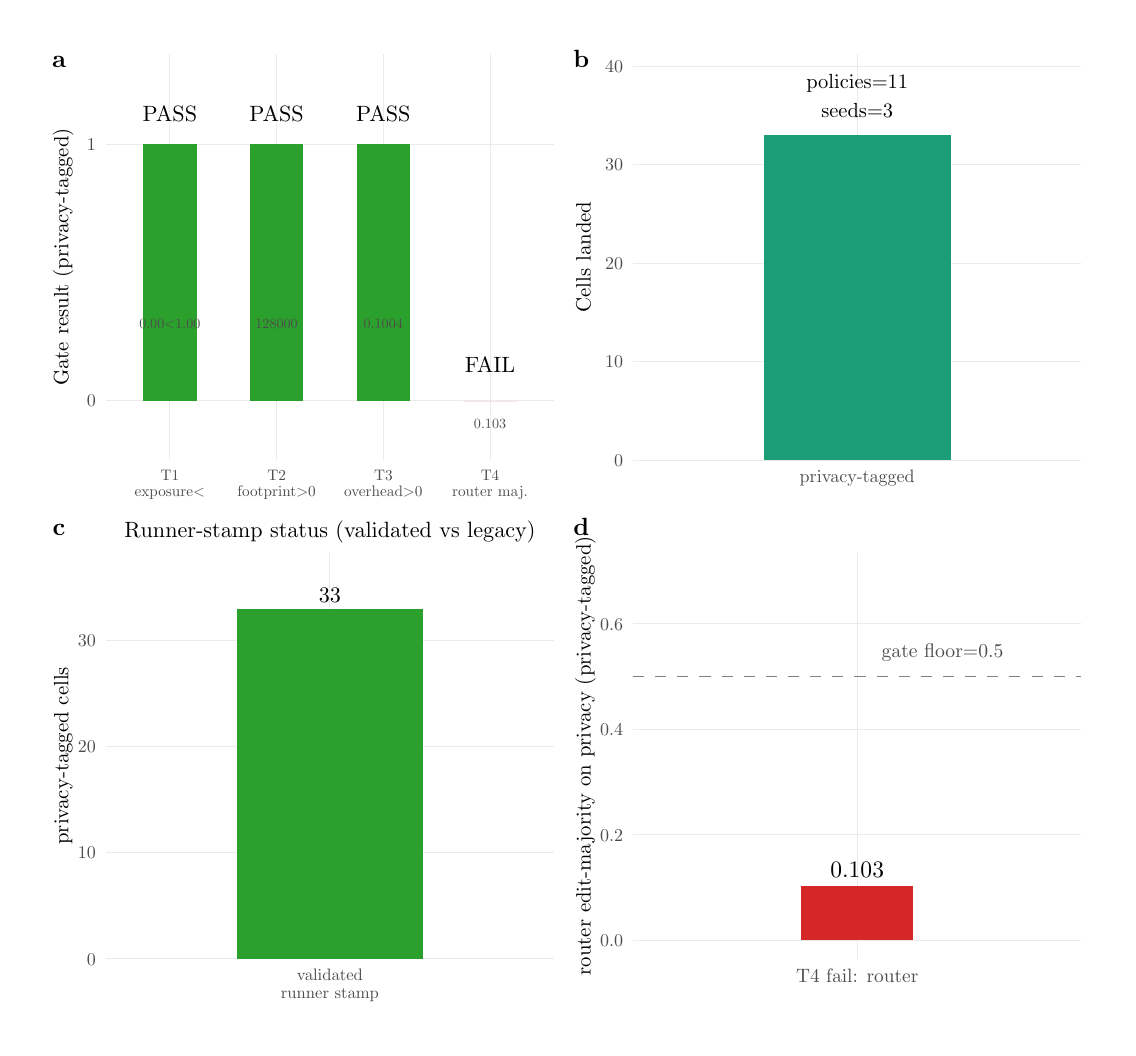
\begin{tikzpicture}[x=1pt,y=1pt]
\definecolor{fillColor}{RGB}{255,255,255}
\path[use as bounding box,fill=fillColor,fill opacity=0.00] (0,0) rectangle (390.26,361.35);
\begin{scope}
\path[clip] (  0.00,  0.00) rectangle (390.26,361.35);
\definecolor{drawColor}{RGB}{255,255,255}
\definecolor{fillColor}{RGB}{255,255,255}

\path[draw=drawColor,line width= 0.6pt,line join=round,line cap=round,fill=fillColor] (  0.00,  0.00) rectangle (390.26,361.35);
\end{scope}
\begin{scope}
\path[clip] (  5.50,186.70) rectangle (194.23,355.85);
\definecolor{fillColor}{RGB}{255,255,255}

\path[fill=fillColor] (  5.50,186.70) rectangle (194.23,355.85);
\end{scope}
\begin{scope}
\path[clip] (194.23,186.70) rectangle (384.76,355.85);
\definecolor{fillColor}{RGB}{255,255,255}

\path[fill=fillColor] (194.23,186.70) rectangle (384.76,355.85);
\end{scope}
\begin{scope}
\path[clip] (  5.50,  5.50) rectangle (194.23,186.70);
\definecolor{fillColor}{RGB}{255,255,255}

\path[fill=fillColor] (  5.50,  5.50) rectangle (194.23,186.70);
\end{scope}
\begin{scope}
\path[clip] (194.23,  5.50) rectangle (384.76,186.70);
\definecolor{fillColor}{RGB}{255,255,255}

\path[fill=fillColor] (194.23,  5.50) rectangle (384.76,186.70);
\end{scope}
\begin{scope}
\path[clip] ( 28.22,205.10) rectangle (190.23,351.85);
\definecolor{drawColor}{gray}{0.92}

\path[draw=drawColor,line width= 0.4pt,line join=round] ( 28.22,226.59) --
	(190.23,226.59);

\path[draw=drawColor,line width= 0.4pt,line join=round] ( 28.22,319.24) --
	(190.23,319.24);

\path[draw=drawColor,line width= 0.4pt,line join=round] ( 51.37,205.10) --
	( 51.37,351.85);

\path[draw=drawColor,line width= 0.4pt,line join=round] ( 89.94,205.10) --
	( 89.94,351.85);

\path[draw=drawColor,line width= 0.4pt,line join=round] (128.51,205.10) --
	(128.51,351.85);

\path[draw=drawColor,line width= 0.4pt,line join=round] (167.08,205.10) --
	(167.08,351.85);
\definecolor{fillColor}{RGB}{44,160,44}

\path[fill=fillColor] ( 41.72,226.59) rectangle ( 61.01,319.24);

\path[fill=fillColor] ( 80.29,226.59) rectangle ( 99.58,319.24);

\path[fill=fillColor] (118.87,226.59) rectangle (138.15,319.24);
\definecolor{fillColor}{RGB}{214,39,40}

\path[fill=fillColor] (157.44,226.59) rectangle (176.73,226.59);
\definecolor{drawColor}{RGB}{0,0,0}

\node[text=drawColor,anchor=base,inner sep=0pt, outer sep=0pt, scale=  0.80] at ( 51.37,327.61) {PASS};

\node[text=drawColor,anchor=base,inner sep=0pt, outer sep=0pt, scale=  0.80] at ( 89.94,327.61) {PASS};

\node[text=drawColor,anchor=base,inner sep=0pt, outer sep=0pt, scale=  0.80] at (128.51,327.61) {PASS};

\node[text=drawColor,anchor=base,inner sep=0pt, outer sep=0pt, scale=  0.80] at (167.08,236.82) {FAIL};
\definecolor{drawColor}{gray}{0.30}

\node[text=drawColor,anchor=base,inner sep=0pt, outer sep=0pt, scale=  0.51] at ( 51.37,252.62) {0.00$<$1.00};

\node[text=drawColor,anchor=base,inner sep=0pt, outer sep=0pt, scale=  0.51] at ( 89.94,252.62) {128000};

\node[text=drawColor,anchor=base,inner sep=0pt, outer sep=0pt, scale=  0.51] at (128.51,252.62) {0.1004};

\node[text=drawColor,anchor=base,inner sep=0pt, outer sep=0pt, scale=  0.51] at (167.08,216.49) {0.103};
\end{scope}
\begin{scope}
\path[clip] (  0.00,  0.00) rectangle (390.26,361.35);
\definecolor{drawColor}{gray}{0.30}

\node[text=drawColor,anchor=base east,inner sep=0pt, outer sep=0pt, scale=  0.65] at ( 24.62,224.35) {0};

\node[text=drawColor,anchor=base east,inner sep=0pt, outer sep=0pt, scale=  0.65] at ( 24.62,317.00) {1};
\end{scope}
\begin{scope}
\path[clip] (  0.00,  0.00) rectangle (390.26,361.35);
\definecolor{drawColor}{gray}{0.30}

\node[text=drawColor,anchor=base,inner sep=0pt, outer sep=0pt, scale=  0.55] at ( 51.37,197.71) {T1};

\node[text=drawColor,anchor=base,inner sep=0pt, outer sep=0pt, scale=  0.55] at ( 51.37,191.77) {exposure$<$};

\node[text=drawColor,anchor=base,inner sep=0pt, outer sep=0pt, scale=  0.55] at ( 89.94,197.71) {T2};

\node[text=drawColor,anchor=base,inner sep=0pt, outer sep=0pt, scale=  0.55] at ( 89.94,191.77) {footprint$>$0};

\node[text=drawColor,anchor=base,inner sep=0pt, outer sep=0pt, scale=  0.55] at (128.51,197.71) {T3};

\node[text=drawColor,anchor=base,inner sep=0pt, outer sep=0pt, scale=  0.55] at (128.51,191.77) {overhead$>$0};

\node[text=drawColor,anchor=base,inner sep=0pt, outer sep=0pt, scale=  0.55] at (167.08,197.71) {T4};

\node[text=drawColor,anchor=base,inner sep=0pt, outer sep=0pt, scale=  0.55] at (167.08,191.77) {router maj.};
\end{scope}
\begin{scope}
\path[clip] (  0.00,  0.00) rectangle (390.26,361.35);
\definecolor{drawColor}{RGB}{0,0,0}

\node[text=drawColor,rotate= 90.00,anchor=base,inner sep=0pt, outer sep=0pt, scale=  0.75] at ( 14.67,278.47) {Gate result (privacy-tagged)};
\end{scope}
\begin{scope}
\path[clip] (  0.00,  0.00) rectangle (390.26,361.35);
\definecolor{drawColor}{RGB}{0,0,0}

\node[text=drawColor,anchor=base,inner sep=0pt, outer sep=0pt, scale=  0.90] at ( 11.31,347.13) {\bfseries a};
\end{scope}
\begin{scope}
\path[clip] (218.75,205.10) rectangle (380.76,351.85);
\definecolor{drawColor}{gray}{0.92}

\path[draw=drawColor,line width= 0.4pt,line join=round] (218.75,205.10) --
	(380.76,205.10);

\path[draw=drawColor,line width= 0.4pt,line join=round] (218.75,240.67) --
	(380.76,240.67);

\path[draw=drawColor,line width= 0.4pt,line join=round] (218.75,276.25) --
	(380.76,276.25);

\path[draw=drawColor,line width= 0.4pt,line join=round] (218.75,311.83) --
	(380.76,311.83);

\path[draw=drawColor,line width= 0.4pt,line join=round] (218.75,347.40) --
	(380.76,347.40);

\path[draw=drawColor,line width= 0.4pt,line join=round] (299.76,205.10) --
	(299.76,351.85);
\definecolor{fillColor}{RGB}{27,158,119}

\path[fill=fillColor] (266.00,205.10) rectangle (333.51,322.50);
\definecolor{drawColor}{RGB}{0,0,0}

\node[text=drawColor,anchor=base,inner sep=0pt, outer sep=0pt, scale=  0.74] at (299.76,339.45) {policies=11};

\node[text=drawColor,anchor=base,inner sep=0pt, outer sep=0pt, scale=  0.74] at (299.76,328.80) {seeds=3};
\end{scope}
\begin{scope}
\path[clip] (  0.00,  0.00) rectangle (390.26,361.35);
\definecolor{drawColor}{gray}{0.30}

\node[text=drawColor,anchor=base east,inner sep=0pt, outer sep=0pt, scale=  0.65] at (215.15,202.86) {0};

\node[text=drawColor,anchor=base east,inner sep=0pt, outer sep=0pt, scale=  0.65] at (215.15,238.43) {10};

\node[text=drawColor,anchor=base east,inner sep=0pt, outer sep=0pt, scale=  0.65] at (215.15,274.01) {20};

\node[text=drawColor,anchor=base east,inner sep=0pt, outer sep=0pt, scale=  0.65] at (215.15,309.59) {30};

\node[text=drawColor,anchor=base east,inner sep=0pt, outer sep=0pt, scale=  0.65] at (215.15,345.16) {40};
\end{scope}
\begin{scope}
\path[clip] (  0.00,  0.00) rectangle (390.26,361.35);
\definecolor{drawColor}{gray}{0.30}

\node[text=drawColor,anchor=base,inner sep=0pt, outer sep=0pt, scale=  0.65] at (299.76,197.02) {privacy-tagged};
\end{scope}
\begin{scope}
\path[clip] (  0.00,  0.00) rectangle (390.26,361.35);
\definecolor{drawColor}{RGB}{0,0,0}

\node[text=drawColor,rotate= 90.00,anchor=base,inner sep=0pt, outer sep=0pt, scale=  0.75] at (203.39,278.47) {Cells landed};
\end{scope}
\begin{scope}
\path[clip] (  0.00,  0.00) rectangle (390.26,361.35);
\definecolor{drawColor}{RGB}{0,0,0}

\node[text=drawColor,anchor=base,inner sep=0pt, outer sep=0pt, scale=  0.90] at (200.05,347.13) {\bfseries b};
\end{scope}
\begin{scope}
\path[clip] ( 28.22, 24.88) rectangle (190.23,171.63);
\definecolor{drawColor}{gray}{0.92}

\path[draw=drawColor,line width= 0.4pt,line join=round] ( 28.22, 24.88) --
	(190.23, 24.88);

\path[draw=drawColor,line width= 0.4pt,line join=round] ( 28.22, 63.22) --
	(190.23, 63.22);

\path[draw=drawColor,line width= 0.4pt,line join=round] ( 28.22,101.55) --
	(190.23,101.55);

\path[draw=drawColor,line width= 0.4pt,line join=round] ( 28.22,139.89) --
	(190.23,139.89);

\path[draw=drawColor,line width= 0.4pt,line join=round] (109.22, 24.88) --
	(109.22,171.63);
\definecolor{fillColor}{RGB}{44,160,44}

\path[fill=fillColor] ( 75.47, 24.88) rectangle (142.98,151.39);
\definecolor{drawColor}{RGB}{0,0,0}

\node[text=drawColor,anchor=base,inner sep=0pt, outer sep=0pt, scale=  0.80] at (109.22,153.59) {33};
\end{scope}
\begin{scope}
\path[clip] (  0.00,  0.00) rectangle (390.26,361.35);
\definecolor{drawColor}{gray}{0.30}

\node[text=drawColor,anchor=base east,inner sep=0pt, outer sep=0pt, scale=  0.65] at ( 24.62, 22.64) {0};

\node[text=drawColor,anchor=base east,inner sep=0pt, outer sep=0pt, scale=  0.65] at ( 24.62, 60.98) {10};

\node[text=drawColor,anchor=base east,inner sep=0pt, outer sep=0pt, scale=  0.65] at ( 24.62, 99.31) {20};

\node[text=drawColor,anchor=base east,inner sep=0pt, outer sep=0pt, scale=  0.65] at ( 24.62,137.65) {30};
\end{scope}
\begin{scope}
\path[clip] (  0.00,  0.00) rectangle (390.26,361.35);
\definecolor{drawColor}{gray}{0.30}

\node[text=drawColor,anchor=base,inner sep=0pt, outer sep=0pt, scale=  0.60] at (109.22, 17.15) {validated};

\node[text=drawColor,anchor=base,inner sep=0pt, outer sep=0pt, scale=  0.60] at (109.22, 10.67) {runner stamp};
\end{scope}
\begin{scope}
\path[clip] (  0.00,  0.00) rectangle (390.26,361.35);
\definecolor{drawColor}{RGB}{0,0,0}

\node[text=drawColor,rotate= 90.00,anchor=base,inner sep=0pt, outer sep=0pt, scale=  0.75] at ( 14.67, 98.26) {privacy-tagged cells};
\end{scope}
\begin{scope}
\path[clip] (  0.00,  0.00) rectangle (390.26,361.35);
\definecolor{drawColor}{RGB}{0,0,0}

\node[text=drawColor,anchor=base,inner sep=0pt, outer sep=0pt, scale=  0.80] at (109.22,177.19) {Runner-stamp status (validated vs legacy)};
\end{scope}
\begin{scope}
\path[clip] (  0.00,  0.00) rectangle (390.26,361.35);
\definecolor{drawColor}{RGB}{0,0,0}

\node[text=drawColor,anchor=base,inner sep=0pt, outer sep=0pt, scale=  0.90] at ( 11.31,177.86) {\bfseries c};
\end{scope}
\begin{scope}
\path[clip] (218.75, 24.88) rectangle (380.76,171.63);
\definecolor{drawColor}{gray}{0.92}

\path[draw=drawColor,line width= 0.4pt,line join=round] (218.75, 31.55) --
	(380.76, 31.55);

\path[draw=drawColor,line width= 0.4pt,line join=round] (218.75, 69.67) --
	(380.76, 69.67);

\path[draw=drawColor,line width= 0.4pt,line join=round] (218.75,107.79) --
	(380.76,107.79);

\path[draw=drawColor,line width= 0.4pt,line join=round] (218.75,145.90) --
	(380.76,145.90);

\path[draw=drawColor,line width= 0.4pt,line join=round] (299.76, 24.88) --
	(299.76,171.63);
\definecolor{fillColor}{RGB}{214,39,40}

\path[fill=fillColor] (279.51, 31.55) rectangle (320.01, 51.19);
\definecolor{drawColor}{gray}{0.50}

\path[draw=drawColor,line width= 0.5pt,dash pattern=on 4pt off 4pt ,line join=round] (218.75,126.84) -- (380.76,126.84);
\definecolor{drawColor}{gray}{0.30}

\node[text=drawColor,anchor=base west,inner sep=0pt, outer sep=0pt, scale=  0.71] at (308.57,133.92) {gate floor=0.5};
\definecolor{drawColor}{RGB}{0,0,0}

\node[text=drawColor,anchor=base,inner sep=0pt, outer sep=0pt, scale=  0.85] at (299.76, 54.13) {0.103};
\end{scope}
\begin{scope}
\path[clip] (  0.00,  0.00) rectangle (390.26,361.35);
\definecolor{drawColor}{gray}{0.30}

\node[text=drawColor,anchor=base east,inner sep=0pt, outer sep=0pt, scale=  0.65] at (215.15, 29.31) {0.0};

\node[text=drawColor,anchor=base east,inner sep=0pt, outer sep=0pt, scale=  0.65] at (215.15, 67.43) {0.2};

\node[text=drawColor,anchor=base east,inner sep=0pt, outer sep=0pt, scale=  0.65] at (215.15,105.55) {0.4};

\node[text=drawColor,anchor=base east,inner sep=0pt, outer sep=0pt, scale=  0.65] at (215.15,143.67) {0.6};
\end{scope}
\begin{scope}
\path[clip] (  0.00,  0.00) rectangle (390.26,361.35);
\definecolor{drawColor}{gray}{0.30}

\node[text=drawColor,anchor=base,inner sep=0pt, outer sep=0pt, scale=  0.70] at (299.76, 16.46) {T4 fail: router};
\end{scope}
\begin{scope}
\path[clip] (  0.00,  0.00) rectangle (390.26,361.35);
\definecolor{drawColor}{RGB}{0,0,0}

\node[text=drawColor,rotate= 90.00,anchor=base,inner sep=0pt, outer sep=0pt, scale=  0.75] at (203.39, 98.26) {router edit-majority on privacy (privacy-tagged)};
\end{scope}
\begin{scope}
\path[clip] (  0.00,  0.00) rectangle (390.26,361.35);
\definecolor{drawColor}{RGB}{0,0,0}

\node[text=drawColor,anchor=base,inner sep=0pt, outer sep=0pt, scale=  0.90] at (200.05,177.86) {\bfseries d};
\end{scope}
\end{tikzpicture}

\caption{Pre-registered gate-status summary across stream configurations. Figure regenerated from canonical measurement artifacts.}
\label{fig:gatestatus}
\end{figure}

\begin{figure}[t]
\centering
% SOURCE: edit-harness/results/frame_a/cells/cell_*_real_MIX_B_*.json
% !TEX encoding = UTF-8 Unicode
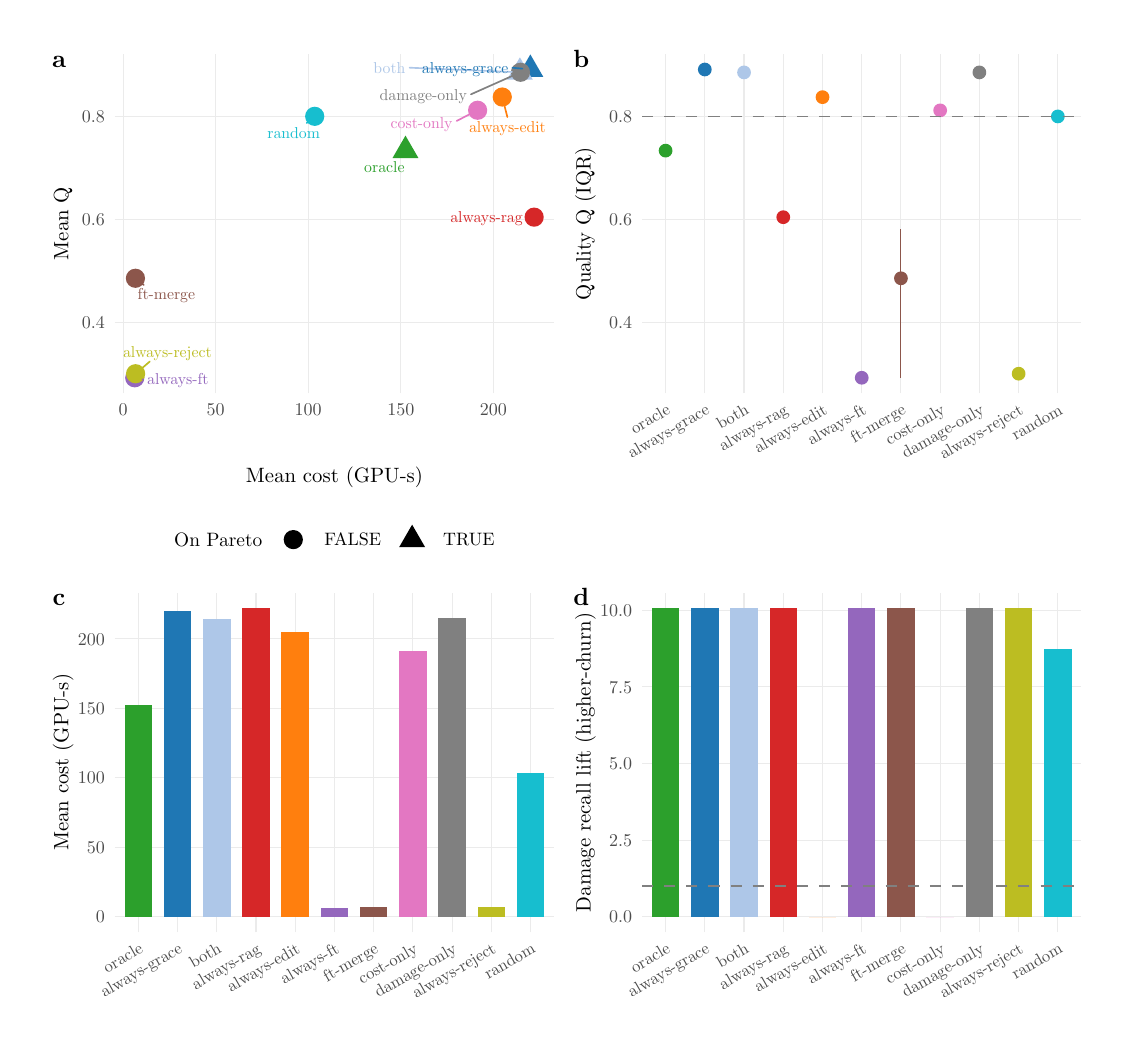
\begin{tikzpicture}[x=1pt,y=1pt]
\definecolor{fillColor}{RGB}{255,255,255}
\path[use as bounding box,fill=fillColor,fill opacity=0.00] (0,0) rectangle (390.26,361.35);
\begin{scope}
\path[clip] (  0.00,  0.00) rectangle (390.26,361.35);
\definecolor{drawColor}{RGB}{255,255,255}
\definecolor{fillColor}{RGB}{255,255,255}

\path[draw=drawColor,line width= 0.6pt,line join=round,line cap=round,fill=fillColor] (  0.00,  0.00) rectangle (390.26,361.35);
\end{scope}
\begin{scope}
\path[clip] (  5.50,161.14) rectangle (194.23,355.85);
\definecolor{fillColor}{RGB}{255,255,255}

\path[fill=fillColor] (  5.50,161.14) rectangle (194.23,355.85);
\end{scope}
\begin{scope}
\path[clip] (194.23,161.14) rectangle (384.76,355.85);
\definecolor{fillColor}{RGB}{255,255,255}

\path[fill=fillColor] (194.23,161.14) rectangle (384.76,355.85);
\end{scope}
\begin{scope}
\path[clip] (  5.50,  5.50) rectangle (194.23,161.14);
\definecolor{fillColor}{RGB}{255,255,255}

\path[fill=fillColor] (  5.50,  5.50) rectangle (194.23,161.14);
\end{scope}
\begin{scope}
\path[clip] (194.23,  5.50) rectangle (384.76,161.14);
\definecolor{fillColor}{RGB}{255,255,255}

\path[fill=fillColor] (194.23,  5.50) rectangle (384.76,161.14);
\end{scope}
\begin{scope}
\path[clip] ( 31.47,229.26) rectangle (190.23,351.85);
\definecolor{drawColor}{gray}{0.92}

\path[draw=drawColor,line width= 0.4pt,line join=round] ( 31.47,254.91) --
	(190.23,254.91);

\path[draw=drawColor,line width= 0.4pt,line join=round] ( 31.47,292.13) --
	(190.23,292.13);

\path[draw=drawColor,line width= 0.4pt,line join=round] ( 31.47,329.36) --
	(190.23,329.36);

\path[draw=drawColor,line width= 0.4pt,line join=round] ( 34.50,229.26) --
	( 34.50,351.85);

\path[draw=drawColor,line width= 0.4pt,line join=round] ( 67.94,229.26) --
	( 67.94,351.85);

\path[draw=drawColor,line width= 0.4pt,line join=round] (101.38,229.26) --
	(101.38,351.85);

\path[draw=drawColor,line width= 0.4pt,line join=round] (134.82,229.26) --
	(134.82,351.85);

\path[draw=drawColor,line width= 0.4pt,line join=round] (168.26,229.26) --
	(168.26,351.85);
\definecolor{fillColor}{RGB}{44,160,44}

\path[fill=fillColor] (136.52,322.35) --
	(141.19,314.25) --
	(131.84,314.25) --
	cycle;
\definecolor{fillColor}{RGB}{31,119,180}

\path[fill=fillColor] (181.64,351.68) --
	(186.31,343.58) --
	(176.96,343.58) --
	cycle;
\definecolor{fillColor}{RGB}{174,199,232}

\path[fill=fillColor] (177.86,350.63) --
	(182.54,342.53) --
	(173.19,342.53) --
	cycle;
\definecolor{fillColor}{RGB}{214,39,40}

\path[fill=fillColor] (183.01,292.88) circle (  3.47);
\definecolor{fillColor}{RGB}{255,127,14}

\path[fill=fillColor] (171.50,336.28) circle (  3.47);
\definecolor{fillColor}{RGB}{148,103,189}

\path[fill=fillColor] ( 38.69,234.83) circle (  3.47);
\definecolor{fillColor}{RGB}{140,86,75}

\path[fill=fillColor] ( 38.94,270.79) circle (  3.47);
\definecolor{fillColor}{RGB}{227,119,194}

\path[fill=fillColor] (162.58,331.50) circle (  3.47);
\definecolor{fillColor}{gray}{0.50}

\path[fill=fillColor] (178.07,345.23) circle (  3.47);
\definecolor{fillColor}{RGB}{188,189,34}

\path[fill=fillColor] ( 39.00,236.30) circle (  3.47);
\definecolor{fillColor}{RGB}{23,190,207}

\path[fill=fillColor] (103.72,329.31) circle (  3.47);
\definecolor{drawColor}{RGB}{44,160,44}

\path[draw=drawColor,line width= 0.6pt,line join=round,line cap=round] (133.63,314.53) -- (134.31,315.10);
\definecolor{drawColor}{RGB}{31,119,180}

\path[draw=drawColor,line width= 0.6pt,line join=round,line cap=round] (175.17,346.87) -- (178.77,346.54);
\definecolor{drawColor}{RGB}{174,199,232}

\path[draw=drawColor,line width= 0.6pt,line join=round,line cap=round] (138.00,346.88) -- (174.99,345.35);
\definecolor{drawColor}{RGB}{255,127,14}

\path[draw=drawColor,line width= 0.6pt,line join=round,line cap=round] (173.33,329.06) -- (172.21,333.49);
\definecolor{drawColor}{RGB}{148,103,189}

\path[draw=drawColor,line width= 0.6pt,line join=round,line cap=round] ( 41.68,234.25) -- ( 41.51,234.28);
\definecolor{drawColor}{RGB}{140,86,75}

\path[draw=drawColor,line width= 0.6pt,line join=round,line cap=round] ( 41.95,268.38) -- ( 41.19,268.99);
\definecolor{drawColor}{RGB}{227,119,194}

\path[draw=drawColor,line width= 0.6pt,line join=round,line cap=round] (155.02,327.66) -- (160.02,330.20);
\definecolor{drawColor}{gray}{0.50}

\path[draw=drawColor,line width= 0.6pt,line join=round,line cap=round] (160.17,337.26) -- (175.44,344.06);
\definecolor{drawColor}{RGB}{188,189,34}

\path[draw=drawColor,line width= 0.6pt,line join=round,line cap=round] ( 44.11,240.70) -- ( 41.18,238.18);
\definecolor{drawColor}{RGB}{23,190,207}

\path[draw=drawColor,line width= 0.6pt,line join=round,line cap=round] (100.84,326.90) -- (101.51,327.47);
\definecolor{drawColor}{RGB}{44,160,44}

\node[text=drawColor,anchor=base,inner sep=0pt, outer sep=0pt, scale=  0.57] at (128.90,309.11) {oracle};
\definecolor{drawColor}{RGB}{31,119,180}

\node[text=drawColor,anchor=base,inner sep=0pt, outer sep=0pt, scale=  0.57] at (158.07,344.92) {always-grace};
\definecolor{drawColor}{RGB}{174,199,232}

\node[text=drawColor,anchor=base,inner sep=0pt, outer sep=0pt, scale=  0.57] at (130.72,344.92) {both};
\definecolor{drawColor}{RGB}{214,39,40}

\node[text=drawColor,anchor=base,inner sep=0pt, outer sep=0pt, scale=  0.57] at (165.81,290.79) {always-rag};
\definecolor{drawColor}{RGB}{255,127,14}

\node[text=drawColor,anchor=base,inner sep=0pt, outer sep=0pt, scale=  0.57] at (173.37,323.63) {always-edit};
\definecolor{drawColor}{RGB}{148,103,189}

\node[text=drawColor,anchor=base,inner sep=0pt, outer sep=0pt, scale=  0.57] at ( 54.27,232.27) {always-ft};
\definecolor{drawColor}{RGB}{140,86,75}

\node[text=drawColor,anchor=base,inner sep=0pt, outer sep=0pt, scale=  0.57] at ( 50.13,262.95) {ft-merge};
\definecolor{drawColor}{RGB}{227,119,194}

\node[text=drawColor,anchor=base,inner sep=0pt, outer sep=0pt, scale=  0.57] at (142.36,325.02) {cost-only};
\definecolor{drawColor}{gray}{0.50}

\node[text=drawColor,anchor=base,inner sep=0pt, outer sep=0pt, scale=  0.57] at (142.94,334.98) {damage-only};
\definecolor{drawColor}{RGB}{188,189,34}

\node[text=drawColor,anchor=base,inner sep=0pt, outer sep=0pt, scale=  0.57] at ( 50.47,242.20) {always-reject};
\definecolor{drawColor}{RGB}{23,190,207}

\node[text=drawColor,anchor=base,inner sep=0pt, outer sep=0pt, scale=  0.57] at ( 96.11,321.48) {random};
\end{scope}
\begin{scope}
\path[clip] (  0.00,  0.00) rectangle (390.26,361.35);
\definecolor{drawColor}{gray}{0.30}

\node[text=drawColor,anchor=base east,inner sep=0pt, outer sep=0pt, scale=  0.65] at ( 27.87,252.67) {0.4};

\node[text=drawColor,anchor=base east,inner sep=0pt, outer sep=0pt, scale=  0.65] at ( 27.87,289.89) {0.6};

\node[text=drawColor,anchor=base east,inner sep=0pt, outer sep=0pt, scale=  0.65] at ( 27.87,327.12) {0.8};
\end{scope}
\begin{scope}
\path[clip] (  0.00,  0.00) rectangle (390.26,361.35);
\definecolor{drawColor}{gray}{0.30}

\node[text=drawColor,anchor=base,inner sep=0pt, outer sep=0pt, scale=  0.65] at ( 34.50,221.18) {0};

\node[text=drawColor,anchor=base,inner sep=0pt, outer sep=0pt, scale=  0.65] at ( 67.94,221.18) {50};

\node[text=drawColor,anchor=base,inner sep=0pt, outer sep=0pt, scale=  0.65] at (101.38,221.18) {100};

\node[text=drawColor,anchor=base,inner sep=0pt, outer sep=0pt, scale=  0.65] at (134.82,221.18) {150};

\node[text=drawColor,anchor=base,inner sep=0pt, outer sep=0pt, scale=  0.65] at (168.26,221.18) {200};
\end{scope}
\begin{scope}
\path[clip] (  0.00,  0.00) rectangle (390.26,361.35);
\definecolor{drawColor}{RGB}{0,0,0}

\node[text=drawColor,anchor=base,inner sep=0pt, outer sep=0pt, scale=  0.75] at (110.85,197.05) {Mean cost (GPU-s)};
\end{scope}
\begin{scope}
\path[clip] (  0.00,  0.00) rectangle (390.26,361.35);
\definecolor{drawColor}{RGB}{0,0,0}

\node[text=drawColor,rotate= 90.00,anchor=base,inner sep=0pt, outer sep=0pt, scale=  0.75] at ( 14.67,290.55) {Mean Q};
\end{scope}
\begin{scope}
\path[clip] (  0.00,  0.00) rectangle (390.26,361.35);
\definecolor{drawColor}{RGB}{0,0,0}

\node[text=drawColor,anchor=base west,inner sep=0pt, outer sep=0pt, scale=  0.70] at ( 52.95,173.95) {On Pareto};
\end{scope}
\begin{scope}
\path[clip] (  0.00,  0.00) rectangle (390.26,361.35);
\definecolor{fillColor}{RGB}{0,0,0}

\path[fill=fillColor] ( 95.98,176.36) circle (  3.47);
\end{scope}
\begin{scope}
\path[clip] (  0.00,  0.00) rectangle (390.26,361.35);
\definecolor{fillColor}{RGB}{0,0,0}

\path[fill=fillColor] (138.92,181.76) --
	(143.60,173.66) --
	(134.25,173.66) --
	cycle;
\end{scope}
\begin{scope}
\path[clip] (  0.00,  0.00) rectangle (390.26,361.35);
\definecolor{drawColor}{RGB}{0,0,0}

\node[text=drawColor,anchor=base west,inner sep=0pt, outer sep=0pt, scale=  0.65] at (107.21,174.12) {FALSE};
\end{scope}
\begin{scope}
\path[clip] (  0.00,  0.00) rectangle (390.26,361.35);
\definecolor{drawColor}{RGB}{0,0,0}

\node[text=drawColor,anchor=base west,inner sep=0pt, outer sep=0pt, scale=  0.65] at (150.15,174.12) {TRUE};
\end{scope}
\begin{scope}
\path[clip] (  0.00,  0.00) rectangle (390.26,361.35);
\definecolor{drawColor}{RGB}{0,0,0}

\node[text=drawColor,anchor=base,inner sep=0pt, outer sep=0pt, scale=  0.90] at ( 11.31,346.88) {\bfseries a};
\end{scope}
\begin{scope}
\path[clip] (222.00,229.26) rectangle (380.76,351.85);
\definecolor{drawColor}{gray}{0.92}

\path[draw=drawColor,line width= 0.4pt,line join=round] (222.00,254.91) --
	(380.76,254.91);

\path[draw=drawColor,line width= 0.4pt,line join=round] (222.00,292.11) --
	(380.76,292.11);

\path[draw=drawColor,line width= 0.4pt,line join=round] (222.00,329.32) --
	(380.76,329.32);

\path[draw=drawColor,line width= 0.4pt,line join=round] (230.51,229.26) --
	(230.51,351.85);

\path[draw=drawColor,line width= 0.4pt,line join=round] (244.68,229.26) --
	(244.68,351.85);

\path[draw=drawColor,line width= 0.4pt,line join=round] (258.86,229.26) --
	(258.86,351.85);

\path[draw=drawColor,line width= 0.4pt,line join=round] (273.03,229.26) --
	(273.03,351.85);

\path[draw=drawColor,line width= 0.4pt,line join=round] (287.21,229.26) --
	(287.21,351.85);

\path[draw=drawColor,line width= 0.4pt,line join=round] (301.38,229.26) --
	(301.38,351.85);

\path[draw=drawColor,line width= 0.4pt,line join=round] (315.55,229.26) --
	(315.55,351.85);

\path[draw=drawColor,line width= 0.4pt,line join=round] (329.73,229.26) --
	(329.73,351.85);

\path[draw=drawColor,line width= 0.4pt,line join=round] (343.90,229.26) --
	(343.90,351.85);

\path[draw=drawColor,line width= 0.4pt,line join=round] (358.08,229.26) --
	(358.08,351.85);

\path[draw=drawColor,line width= 0.4pt,line join=round] (372.25,229.26) --
	(372.25,351.85);
\definecolor{drawColor}{RGB}{44,160,44}

\path[draw=drawColor,line width= 0.4pt,line join=round] (230.51,316.81) -- (230.51,317.04);
\definecolor{drawColor}{RGB}{31,119,180}

\path[draw=drawColor,line width= 0.4pt,line join=round] (244.68,346.13) -- (244.68,346.28);
\definecolor{drawColor}{RGB}{174,199,232}

\path[draw=drawColor,line width= 0.4pt,line join=round] (258.86,345.08) -- (258.86,345.26);
\definecolor{drawColor}{RGB}{214,39,40}

\path[draw=drawColor,line width= 0.4pt,line join=round] (273.03,292.78) -- (273.03,293.00);
\definecolor{drawColor}{RGB}{255,127,14}

\path[draw=drawColor,line width= 0.4pt,line join=round] (287.21,335.69) -- (287.21,336.59);
\definecolor{drawColor}{RGB}{148,103,189}

\path[draw=drawColor,line width= 0.4pt,line join=round] (301.38,234.83) -- (301.38,234.85);
\definecolor{drawColor}{RGB}{140,86,75}

\path[draw=drawColor,line width= 0.4pt,line join=round] (315.55,234.85) -- (315.55,288.75);
\definecolor{drawColor}{RGB}{227,119,194}

\path[draw=drawColor,line width= 0.4pt,line join=round] (329.73,331.01) -- (329.73,332.10);
\definecolor{drawColor}{gray}{0.50}

\path[draw=drawColor,line width= 0.4pt,line join=round] (343.90,345.08) -- (343.90,345.26);
\definecolor{drawColor}{RGB}{188,189,34}

\path[draw=drawColor,line width= 0.4pt,line join=round] (358.08,236.31) -- (358.08,236.31);
\definecolor{drawColor}{RGB}{23,190,207}

\path[draw=drawColor,line width= 0.4pt,line join=round] (372.25,328.54) -- (372.25,330.01);
\definecolor{drawColor}{RGB}{44,160,44}
\definecolor{fillColor}{RGB}{44,160,44}

\path[draw=drawColor,line width= 0.5pt,line join=round,line cap=round,fill=fillColor] (230.51,316.91) circle (  2.23);
\definecolor{drawColor}{RGB}{31,119,180}
\definecolor{fillColor}{RGB}{31,119,180}

\path[draw=drawColor,line width= 0.5pt,line join=round,line cap=round,fill=fillColor] (244.68,346.23) circle (  2.23);
\definecolor{drawColor}{RGB}{174,199,232}
\definecolor{fillColor}{RGB}{174,199,232}

\path[draw=drawColor,line width= 0.5pt,line join=round,line cap=round,fill=fillColor] (258.86,345.18) circle (  2.23);
\definecolor{drawColor}{RGB}{214,39,40}
\definecolor{fillColor}{RGB}{214,39,40}

\path[draw=drawColor,line width= 0.5pt,line join=round,line cap=round,fill=fillColor] (273.03,292.86) circle (  2.23);
\definecolor{drawColor}{RGB}{255,127,14}
\definecolor{fillColor}{RGB}{255,127,14}

\path[draw=drawColor,line width= 0.5pt,line join=round,line cap=round,fill=fillColor] (287.21,336.24) circle (  2.23);
\definecolor{drawColor}{RGB}{148,103,189}
\definecolor{fillColor}{RGB}{148,103,189}

\path[draw=drawColor,line width= 0.5pt,line join=round,line cap=round,fill=fillColor] (301.38,234.84) circle (  2.23);
\definecolor{drawColor}{RGB}{140,86,75}
\definecolor{fillColor}{RGB}{140,86,75}

\path[draw=drawColor,line width= 0.5pt,line join=round,line cap=round,fill=fillColor] (315.55,270.78) circle (  2.23);
\definecolor{drawColor}{RGB}{227,119,194}
\definecolor{fillColor}{RGB}{227,119,194}

\path[draw=drawColor,line width= 0.5pt,line join=round,line cap=round,fill=fillColor] (329.73,331.46) circle (  2.23);
\definecolor{drawColor}{gray}{0.50}
\definecolor{fillColor}{gray}{0.50}

\path[draw=drawColor,line width= 0.5pt,line join=round,line cap=round,fill=fillColor] (343.90,345.18) circle (  2.23);
\definecolor{drawColor}{RGB}{188,189,34}
\definecolor{fillColor}{RGB}{188,189,34}

\path[draw=drawColor,line width= 0.5pt,line join=round,line cap=round,fill=fillColor] (358.08,236.31) circle (  2.23);
\definecolor{drawColor}{RGB}{23,190,207}
\definecolor{fillColor}{RGB}{23,190,207}

\path[draw=drawColor,line width= 0.5pt,line join=round,line cap=round,fill=fillColor] (372.25,329.27) circle (  2.23);
\definecolor{drawColor}{gray}{0.50}

\path[draw=drawColor,line width= 0.5pt,dash pattern=on 4pt off 4pt ,line join=round] (222.00,329.27) -- (380.76,329.27);
\end{scope}
\begin{scope}
\path[clip] (  0.00,  0.00) rectangle (390.26,361.35);
\definecolor{drawColor}{gray}{0.30}

\node[text=drawColor,anchor=base east,inner sep=0pt, outer sep=0pt, scale=  0.65] at (218.40,252.67) {0.4};

\node[text=drawColor,anchor=base east,inner sep=0pt, outer sep=0pt, scale=  0.65] at (218.40,289.87) {0.6};

\node[text=drawColor,anchor=base east,inner sep=0pt, outer sep=0pt, scale=  0.65] at (218.40,327.08) {0.8};
\end{scope}
\begin{scope}
\path[clip] (  0.00,  0.00) rectangle (390.26,361.35);
\definecolor{drawColor}{gray}{0.30}

\node[text=drawColor,rotate= 30.00,anchor=base east,inner sep=0pt, outer sep=0pt, scale=  0.60] at (232.57,222.08) {oracle};

\node[text=drawColor,rotate= 30.00,anchor=base east,inner sep=0pt, outer sep=0pt, scale=  0.60] at (246.75,222.08) {always-grace};

\node[text=drawColor,rotate= 30.00,anchor=base east,inner sep=0pt, outer sep=0pt, scale=  0.60] at (260.92,222.08) {both};

\node[text=drawColor,rotate= 30.00,anchor=base east,inner sep=0pt, outer sep=0pt, scale=  0.60] at (275.10,222.08) {always-rag};

\node[text=drawColor,rotate= 30.00,anchor=base east,inner sep=0pt, outer sep=0pt, scale=  0.60] at (289.27,222.08) {always-edit};

\node[text=drawColor,rotate= 30.00,anchor=base east,inner sep=0pt, outer sep=0pt, scale=  0.60] at (303.45,222.08) {always-ft};

\node[text=drawColor,rotate= 30.00,anchor=base east,inner sep=0pt, outer sep=0pt, scale=  0.60] at (317.62,222.08) {ft-merge};

\node[text=drawColor,rotate= 30.00,anchor=base east,inner sep=0pt, outer sep=0pt, scale=  0.60] at (331.80,222.08) {cost-only};

\node[text=drawColor,rotate= 30.00,anchor=base east,inner sep=0pt, outer sep=0pt, scale=  0.60] at (345.97,222.08) {damage-only};

\node[text=drawColor,rotate= 30.00,anchor=base east,inner sep=0pt, outer sep=0pt, scale=  0.60] at (360.14,222.08) {always-reject};

\node[text=drawColor,rotate= 30.00,anchor=base east,inner sep=0pt, outer sep=0pt, scale=  0.60] at (374.32,222.08) {random};
\end{scope}
\begin{scope}
\path[clip] (  0.00,  0.00) rectangle (390.26,361.35);
\definecolor{drawColor}{RGB}{0,0,0}

\node[text=drawColor,rotate= 90.00,anchor=base,inner sep=0pt, outer sep=0pt, scale=  0.75] at (203.39,290.55) {Quality Q (IQR)};
\end{scope}
\begin{scope}
\path[clip] (  0.00,  0.00) rectangle (390.26,361.35);
\definecolor{drawColor}{RGB}{0,0,0}

\node[text=drawColor,anchor=base,inner sep=0pt, outer sep=0pt, scale=  0.90] at (200.05,346.88) {\bfseries b};
\end{scope}
\begin{scope}
\path[clip] ( 31.47, 34.54) rectangle (190.23,157.14);
\definecolor{drawColor}{gray}{0.92}

\path[draw=drawColor,line width= 0.4pt,line join=round] ( 31.47, 40.12) --
	(190.23, 40.12);

\path[draw=drawColor,line width= 0.4pt,line join=round] ( 31.47, 65.21) --
	(190.23, 65.21);

\path[draw=drawColor,line width= 0.4pt,line join=round] ( 31.47, 90.30) --
	(190.23, 90.30);

\path[draw=drawColor,line width= 0.4pt,line join=round] ( 31.47,115.40) --
	(190.23,115.40);

\path[draw=drawColor,line width= 0.4pt,line join=round] ( 31.47,140.49) --
	(190.23,140.49);

\path[draw=drawColor,line width= 0.4pt,line join=round] ( 39.98, 34.54) --
	( 39.98,157.14);

\path[draw=drawColor,line width= 0.4pt,line join=round] ( 54.15, 34.54) --
	( 54.15,157.14);

\path[draw=drawColor,line width= 0.4pt,line join=round] ( 68.32, 34.54) --
	( 68.32,157.14);

\path[draw=drawColor,line width= 0.4pt,line join=round] ( 82.50, 34.54) --
	( 82.50,157.14);

\path[draw=drawColor,line width= 0.4pt,line join=round] ( 96.67, 34.54) --
	( 96.67,157.14);

\path[draw=drawColor,line width= 0.4pt,line join=round] (110.85, 34.54) --
	(110.85,157.14);

\path[draw=drawColor,line width= 0.4pt,line join=round] (125.02, 34.54) --
	(125.02,157.14);

\path[draw=drawColor,line width= 0.4pt,line join=round] (139.20, 34.54) --
	(139.20,157.14);

\path[draw=drawColor,line width= 0.4pt,line join=round] (153.37, 34.54) --
	(153.37,157.14);

\path[draw=drawColor,line width= 0.4pt,line join=round] (167.55, 34.54) --
	(167.55,157.14);

\path[draw=drawColor,line width= 0.4pt,line join=round] (181.72, 34.54) --
	(181.72,157.14);
\definecolor{fillColor}{RGB}{44,160,44}

\path[fill=fillColor] ( 35.01, 40.12) rectangle ( 44.94,116.67);
\definecolor{fillColor}{RGB}{31,119,180}

\path[fill=fillColor] ( 49.19, 40.12) rectangle ( 59.11,150.53);
\definecolor{fillColor}{RGB}{174,199,232}

\path[fill=fillColor] ( 63.36, 40.12) rectangle ( 73.29,147.70);
\definecolor{fillColor}{RGB}{214,39,40}

\path[fill=fillColor] ( 77.54, 40.12) rectangle ( 87.46,151.56);
\definecolor{fillColor}{RGB}{255,127,14}

\path[fill=fillColor] ( 91.71, 40.12) rectangle (101.64,142.93);
\definecolor{fillColor}{RGB}{148,103,189}

\path[fill=fillColor] (105.89, 40.12) rectangle (115.81, 43.26);
\definecolor{fillColor}{RGB}{140,86,75}

\path[fill=fillColor] (120.06, 40.12) rectangle (129.98, 43.45);
\definecolor{fillColor}{RGB}{227,119,194}

\path[fill=fillColor] (134.24, 40.12) rectangle (144.16,136.23);
\definecolor{fillColor}{gray}{0.50}

\path[fill=fillColor] (148.41, 40.12) rectangle (158.33,147.86);
\definecolor{fillColor}{RGB}{188,189,34}

\path[fill=fillColor] (162.59, 40.12) rectangle (172.51, 43.49);
\definecolor{fillColor}{RGB}{23,190,207}

\path[fill=fillColor] (176.76, 40.12) rectangle (186.68, 92.06);
\end{scope}
\begin{scope}
\path[clip] (  0.00,  0.00) rectangle (390.26,361.35);
\definecolor{drawColor}{gray}{0.30}

\node[text=drawColor,anchor=base east,inner sep=0pt, outer sep=0pt, scale=  0.65] at ( 27.87, 37.88) {0};

\node[text=drawColor,anchor=base east,inner sep=0pt, outer sep=0pt, scale=  0.65] at ( 27.87, 62.97) {50};

\node[text=drawColor,anchor=base east,inner sep=0pt, outer sep=0pt, scale=  0.65] at ( 27.87, 88.07) {100};

\node[text=drawColor,anchor=base east,inner sep=0pt, outer sep=0pt, scale=  0.65] at ( 27.87,113.16) {150};

\node[text=drawColor,anchor=base east,inner sep=0pt, outer sep=0pt, scale=  0.65] at ( 27.87,138.25) {200};
\end{scope}
\begin{scope}
\path[clip] (  0.00,  0.00) rectangle (390.26,361.35);
\definecolor{drawColor}{gray}{0.30}

\node[text=drawColor,rotate= 30.00,anchor=base east,inner sep=0pt, outer sep=0pt, scale=  0.60] at ( 42.04, 27.36) {oracle};

\node[text=drawColor,rotate= 30.00,anchor=base east,inner sep=0pt, outer sep=0pt, scale=  0.60] at ( 56.22, 27.36) {always-grace};

\node[text=drawColor,rotate= 30.00,anchor=base east,inner sep=0pt, outer sep=0pt, scale=  0.60] at ( 70.39, 27.36) {both};

\node[text=drawColor,rotate= 30.00,anchor=base east,inner sep=0pt, outer sep=0pt, scale=  0.60] at ( 84.57, 27.36) {always-rag};

\node[text=drawColor,rotate= 30.00,anchor=base east,inner sep=0pt, outer sep=0pt, scale=  0.60] at ( 98.74, 27.36) {always-edit};

\node[text=drawColor,rotate= 30.00,anchor=base east,inner sep=0pt, outer sep=0pt, scale=  0.60] at (112.91, 27.36) {always-ft};

\node[text=drawColor,rotate= 30.00,anchor=base east,inner sep=0pt, outer sep=0pt, scale=  0.60] at (127.09, 27.36) {ft-merge};

\node[text=drawColor,rotate= 30.00,anchor=base east,inner sep=0pt, outer sep=0pt, scale=  0.60] at (141.26, 27.36) {cost-only};

\node[text=drawColor,rotate= 30.00,anchor=base east,inner sep=0pt, outer sep=0pt, scale=  0.60] at (155.44, 27.36) {damage-only};

\node[text=drawColor,rotate= 30.00,anchor=base east,inner sep=0pt, outer sep=0pt, scale=  0.60] at (169.61, 27.36) {always-reject};

\node[text=drawColor,rotate= 30.00,anchor=base east,inner sep=0pt, outer sep=0pt, scale=  0.60] at (183.79, 27.36) {random};
\end{scope}
\begin{scope}
\path[clip] (  0.00,  0.00) rectangle (390.26,361.35);
\definecolor{drawColor}{RGB}{0,0,0}

\node[text=drawColor,rotate= 90.00,anchor=base,inner sep=0pt, outer sep=0pt, scale=  0.75] at ( 14.67, 95.84) {Mean cost (GPU-s)};
\end{scope}
\begin{scope}
\path[clip] (  0.00,  0.00) rectangle (390.26,361.35);
\definecolor{drawColor}{RGB}{0,0,0}

\node[text=drawColor,anchor=base,inner sep=0pt, outer sep=0pt, scale=  0.90] at ( 11.31,152.55) {\bfseries c};
\end{scope}
\begin{scope}
\path[clip] (222.00, 34.54) rectangle (380.76,157.14);
\definecolor{drawColor}{gray}{0.92}

\path[draw=drawColor,line width= 0.4pt,line join=round] (222.00, 40.12) --
	(380.76, 40.12);

\path[draw=drawColor,line width= 0.4pt,line join=round] (222.00, 67.78) --
	(380.76, 67.78);

\path[draw=drawColor,line width= 0.4pt,line join=round] (222.00, 95.45) --
	(380.76, 95.45);

\path[draw=drawColor,line width= 0.4pt,line join=round] (222.00,123.12) --
	(380.76,123.12);

\path[draw=drawColor,line width= 0.4pt,line join=round] (222.00,150.78) --
	(380.76,150.78);

\path[draw=drawColor,line width= 0.4pt,line join=round] (230.51, 34.54) --
	(230.51,157.14);

\path[draw=drawColor,line width= 0.4pt,line join=round] (244.68, 34.54) --
	(244.68,157.14);

\path[draw=drawColor,line width= 0.4pt,line join=round] (258.86, 34.54) --
	(258.86,157.14);

\path[draw=drawColor,line width= 0.4pt,line join=round] (273.03, 34.54) --
	(273.03,157.14);

\path[draw=drawColor,line width= 0.4pt,line join=round] (287.21, 34.54) --
	(287.21,157.14);

\path[draw=drawColor,line width= 0.4pt,line join=round] (301.38, 34.54) --
	(301.38,157.14);

\path[draw=drawColor,line width= 0.4pt,line join=round] (315.55, 34.54) --
	(315.55,157.14);

\path[draw=drawColor,line width= 0.4pt,line join=round] (329.73, 34.54) --
	(329.73,157.14);

\path[draw=drawColor,line width= 0.4pt,line join=round] (343.90, 34.54) --
	(343.90,157.14);

\path[draw=drawColor,line width= 0.4pt,line join=round] (358.08, 34.54) --
	(358.08,157.14);

\path[draw=drawColor,line width= 0.4pt,line join=round] (372.25, 34.54) --
	(372.25,157.14);
\definecolor{fillColor}{RGB}{44,160,44}

\path[fill=fillColor] (225.55, 40.12) rectangle (235.47,151.56);
\definecolor{fillColor}{RGB}{31,119,180}

\path[fill=fillColor] (239.72, 40.12) rectangle (249.64,151.56);
\definecolor{fillColor}{RGB}{174,199,232}

\path[fill=fillColor] (253.90, 40.12) rectangle (263.82,151.56);
\definecolor{fillColor}{RGB}{214,39,40}

\path[fill=fillColor] (268.07, 40.12) rectangle (277.99,151.56);
\definecolor{fillColor}{RGB}{255,127,14}

\path[fill=fillColor] (282.24, 40.12) rectangle (292.17, 40.12);
\definecolor{fillColor}{RGB}{148,103,189}

\path[fill=fillColor] (296.42, 40.12) rectangle (306.34,151.56);
\definecolor{fillColor}{RGB}{140,86,75}

\path[fill=fillColor] (310.59, 40.12) rectangle (320.52,151.56);
\definecolor{fillColor}{RGB}{227,119,194}

\path[fill=fillColor] (324.77, 40.12) rectangle (334.69, 40.12);
\definecolor{fillColor}{gray}{0.50}

\path[fill=fillColor] (338.94, 40.12) rectangle (348.87,151.56);
\definecolor{fillColor}{RGB}{188,189,34}

\path[fill=fillColor] (353.12, 40.12) rectangle (363.04,151.56);
\definecolor{fillColor}{RGB}{23,190,207}

\path[fill=fillColor] (367.29, 40.12) rectangle (377.21,136.70);
\definecolor{drawColor}{gray}{0.50}

\path[draw=drawColor,line width= 0.5pt,dash pattern=on 4pt off 4pt ,line join=round] (222.00, 51.18) -- (380.76, 51.18);
\end{scope}
\begin{scope}
\path[clip] (  0.00,  0.00) rectangle (390.26,361.35);
\definecolor{drawColor}{gray}{0.30}

\node[text=drawColor,anchor=base east,inner sep=0pt, outer sep=0pt, scale=  0.65] at (218.40, 37.88) {0.0};

\node[text=drawColor,anchor=base east,inner sep=0pt, outer sep=0pt, scale=  0.65] at (218.40, 65.54) {2.5};

\node[text=drawColor,anchor=base east,inner sep=0pt, outer sep=0pt, scale=  0.65] at (218.40, 93.21) {5.0};

\node[text=drawColor,anchor=base east,inner sep=0pt, outer sep=0pt, scale=  0.65] at (218.40,120.88) {7.5};

\node[text=drawColor,anchor=base east,inner sep=0pt, outer sep=0pt, scale=  0.65] at (218.40,148.55) {10.0};
\end{scope}
\begin{scope}
\path[clip] (  0.00,  0.00) rectangle (390.26,361.35);
\definecolor{drawColor}{gray}{0.30}

\node[text=drawColor,rotate= 30.00,anchor=base east,inner sep=0pt, outer sep=0pt, scale=  0.60] at (232.57, 27.36) {oracle};

\node[text=drawColor,rotate= 30.00,anchor=base east,inner sep=0pt, outer sep=0pt, scale=  0.60] at (246.75, 27.36) {always-grace};

\node[text=drawColor,rotate= 30.00,anchor=base east,inner sep=0pt, outer sep=0pt, scale=  0.60] at (260.92, 27.36) {both};

\node[text=drawColor,rotate= 30.00,anchor=base east,inner sep=0pt, outer sep=0pt, scale=  0.60] at (275.10, 27.36) {always-rag};

\node[text=drawColor,rotate= 30.00,anchor=base east,inner sep=0pt, outer sep=0pt, scale=  0.60] at (289.27, 27.36) {always-edit};

\node[text=drawColor,rotate= 30.00,anchor=base east,inner sep=0pt, outer sep=0pt, scale=  0.60] at (303.45, 27.36) {always-ft};

\node[text=drawColor,rotate= 30.00,anchor=base east,inner sep=0pt, outer sep=0pt, scale=  0.60] at (317.62, 27.36) {ft-merge};

\node[text=drawColor,rotate= 30.00,anchor=base east,inner sep=0pt, outer sep=0pt, scale=  0.60] at (331.80, 27.36) {cost-only};

\node[text=drawColor,rotate= 30.00,anchor=base east,inner sep=0pt, outer sep=0pt, scale=  0.60] at (345.97, 27.36) {damage-only};

\node[text=drawColor,rotate= 30.00,anchor=base east,inner sep=0pt, outer sep=0pt, scale=  0.60] at (360.14, 27.36) {always-reject};

\node[text=drawColor,rotate= 30.00,anchor=base east,inner sep=0pt, outer sep=0pt, scale=  0.60] at (374.32, 27.36) {random};
\end{scope}
\begin{scope}
\path[clip] (  0.00,  0.00) rectangle (390.26,361.35);
\definecolor{drawColor}{RGB}{0,0,0}

\node[text=drawColor,rotate= 90.00,anchor=base,inner sep=0pt, outer sep=0pt, scale=  0.75] at (203.39, 95.84) {Damage recall lift (higher-churn)};
\end{scope}
\begin{scope}
\path[clip] (  0.00,  0.00) rectangle (390.26,361.35);
\definecolor{drawColor}{RGB}{0,0,0}

\node[text=drawColor,anchor=base,inner sep=0pt, outer sep=0pt, scale=  0.90] at (200.05,152.55) {\bfseries d};
\end{scope}
\end{tikzpicture}

\caption{Higher-churn maintenance operating points ($Q$ vs.\ cost) for all policies. Figure regenerated from canonical measurement artifacts.}
\label{fig:higher-churn}
\end{figure}

\begin{figure}[t]
\centering
% SOURCE: edit-harness/results/frame_a/cells/cell_*_real_MIX_C_*.json
% !TEX encoding = UTF-8 Unicode
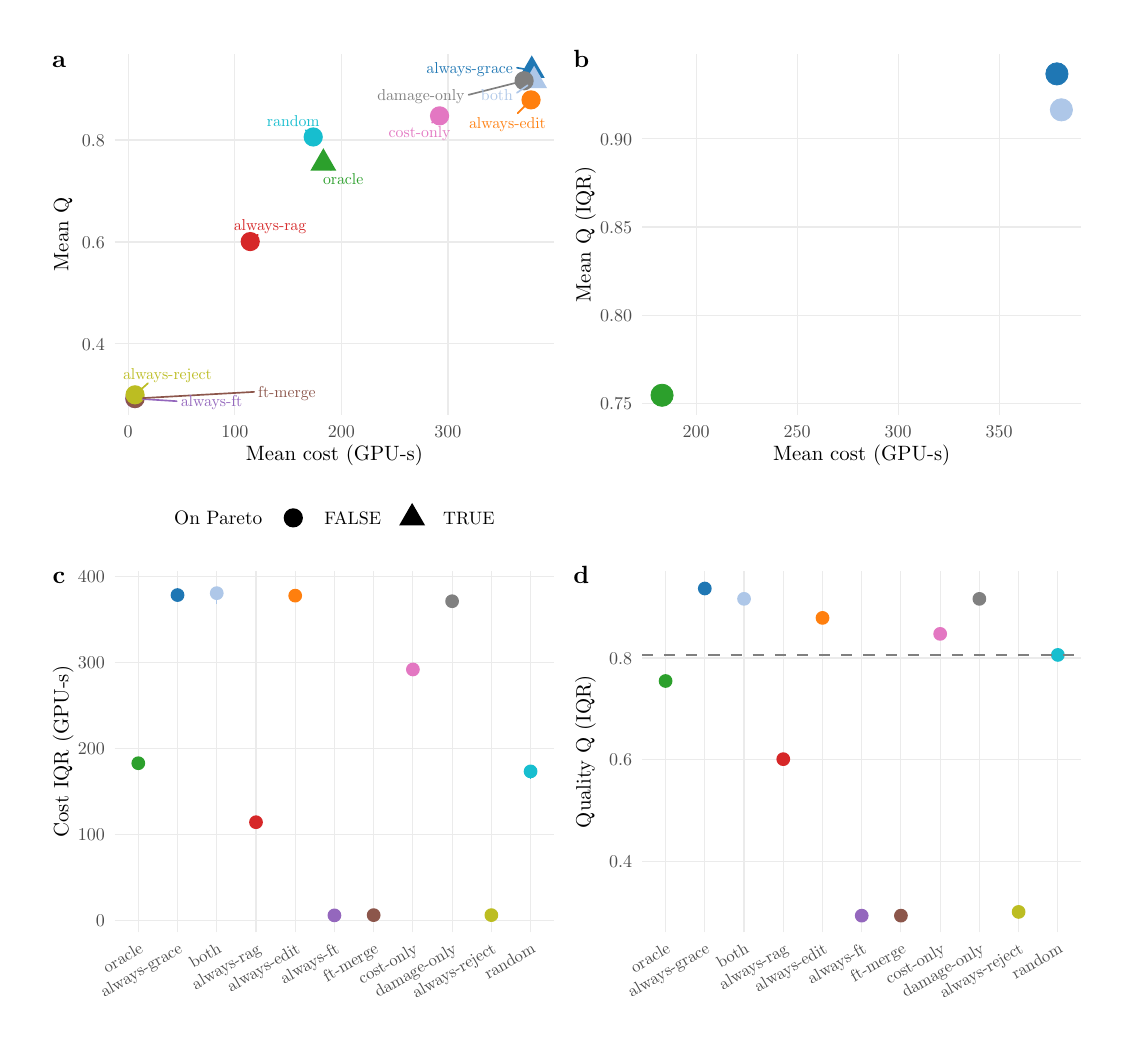
\begin{tikzpicture}[x=1pt,y=1pt]
\definecolor{fillColor}{RGB}{255,255,255}
\path[use as bounding box,fill=fillColor,fill opacity=0.00] (0,0) rectangle (390.26,361.35);
\begin{scope}
\path[clip] (  0.00,  0.00) rectangle (390.26,361.35);
\definecolor{drawColor}{RGB}{255,255,255}
\definecolor{fillColor}{RGB}{255,255,255}

\path[draw=drawColor,line width= 0.6pt,line join=round,line cap=round,fill=fillColor] (  0.00,  0.00) rectangle (390.26,361.35);
\end{scope}
\begin{scope}
\path[clip] (  5.50,168.99) rectangle (194.23,355.85);
\definecolor{fillColor}{RGB}{255,255,255}

\path[fill=fillColor] (  5.50,168.99) rectangle (194.23,355.85);
\end{scope}
\begin{scope}
\path[clip] (194.23,168.99) rectangle (384.76,355.85);
\definecolor{fillColor}{RGB}{255,255,255}

\path[fill=fillColor] (194.23,168.99) rectangle (384.76,355.85);
\end{scope}
\begin{scope}
\path[clip] (  5.50,  5.50) rectangle (194.23,168.99);
\definecolor{fillColor}{RGB}{255,255,255}

\path[fill=fillColor] (  5.50,  5.50) rectangle (194.23,168.99);
\end{scope}
\begin{scope}
\path[clip] (194.23,  5.50) rectangle (384.76,168.99);
\definecolor{fillColor}{RGB}{255,255,255}

\path[fill=fillColor] (194.23,  5.50) rectangle (384.76,168.99);
\end{scope}
\begin{scope}
\path[clip] ( 31.47,221.41) rectangle (190.23,351.85);
\definecolor{drawColor}{gray}{0.92}

\path[draw=drawColor,line width= 0.4pt,line join=round] ( 31.47,247.09) --
	(190.23,247.09);

\path[draw=drawColor,line width= 0.4pt,line join=round] ( 31.47,283.91) --
	(190.23,283.91);

\path[draw=drawColor,line width= 0.4pt,line join=round] ( 31.47,320.74) --
	(190.23,320.74);

\path[draw=drawColor,line width= 0.4pt,line join=round] ( 36.33,221.41) --
	( 36.33,351.85);

\path[draw=drawColor,line width= 0.4pt,line join=round] ( 74.85,221.41) --
	( 74.85,351.85);

\path[draw=drawColor,line width= 0.4pt,line join=round] (113.36,221.41) --
	(113.36,351.85);

\path[draw=drawColor,line width= 0.4pt,line join=round] (151.88,221.41) --
	(151.88,351.85);
\definecolor{fillColor}{RGB}{44,160,44}

\path[fill=fillColor] (106.85,317.79) --
	(111.52,309.69) --
	(102.17,309.69) --
	cycle;
\definecolor{fillColor}{RGB}{31,119,180}

\path[fill=fillColor] (182.15,351.32) --
	(186.83,343.22) --
	(177.48,343.22) --
	cycle;
\definecolor{fillColor}{RGB}{174,199,232}

\path[fill=fillColor] (183.01,347.57) --
	(187.69,339.47) --
	(178.33,339.47) --
	cycle;
\definecolor{fillColor}{RGB}{214,39,40}

\path[fill=fillColor] ( 80.42,284.06) circle (  3.47);
\definecolor{fillColor}{RGB}{255,127,14}

\path[fill=fillColor] (181.89,335.26) circle (  3.47);
\definecolor{fillColor}{RGB}{148,103,189}

\path[fill=fillColor] ( 38.69,227.33) circle (  3.47);
\definecolor{fillColor}{RGB}{140,86,75}

\path[fill=fillColor] ( 38.80,227.33) circle (  3.47);
\definecolor{fillColor}{RGB}{227,119,194}

\path[fill=fillColor] (148.83,329.48) circle (  3.47);
\definecolor{fillColor}{gray}{0.50}

\path[fill=fillColor] (179.39,342.17) circle (  3.47);
\definecolor{fillColor}{RGB}{188,189,34}

\path[fill=fillColor] ( 38.80,228.68) circle (  3.47);
\definecolor{fillColor}{RGB}{23,190,207}

\path[fill=fillColor] (103.18,321.85) circle (  3.47);
\definecolor{drawColor}{RGB}{44,160,44}

\path[draw=drawColor,line width= 0.6pt,line join=round,line cap=round] (109.58,309.96) -- (109.00,310.48);
\definecolor{drawColor}{RGB}{31,119,180}

\path[draw=drawColor,line width= 0.6pt,line join=round,line cap=round] (176.81,346.86) -- (179.32,346.42);
\definecolor{drawColor}{RGB}{174,199,232}

\path[draw=drawColor,line width= 0.6pt,line join=round,line cap=round] (176.79,337.81) -- (180.66,340.52);
\definecolor{drawColor}{RGB}{214,39,40}

\path[draw=drawColor,line width= 0.6pt,line join=round,line cap=round] ( 83.16,286.50) -- ( 82.57,285.97);
\definecolor{drawColor}{RGB}{255,127,14}

\path[draw=drawColor,line width= 0.6pt,line join=round,line cap=round] (177.05,330.43) -- (179.85,333.23);
\definecolor{drawColor}{RGB}{148,103,189}

\path[draw=drawColor,line width= 0.6pt,line join=round,line cap=round] ( 53.86,226.38) -- ( 41.56,227.15);
\definecolor{drawColor}{RGB}{140,86,75}

\path[draw=drawColor,line width= 0.6pt,line join=round,line cap=round] ( 81.83,229.74) -- ( 41.67,227.50);
\definecolor{drawColor}{RGB}{227,119,194}

\path[draw=drawColor,line width= 0.6pt,line join=round,line cap=round] (146.07,327.02) -- (146.68,327.57);
\definecolor{drawColor}{gray}{0.50}

\path[draw=drawColor,line width= 0.6pt,line join=round,line cap=round] (159.32,337.08) -- (176.60,341.46);
\definecolor{drawColor}{RGB}{188,189,34}

\path[draw=drawColor,line width= 0.6pt,line join=round,line cap=round] ( 43.45,232.85) -- ( 40.94,230.60);
\definecolor{drawColor}{RGB}{23,190,207}

\path[draw=drawColor,line width= 0.6pt,line join=round,line cap=round] (100.43,324.29) -- (101.03,323.76);
\definecolor{drawColor}{RGB}{44,160,44}

\node[text=drawColor,anchor=base,inner sep=0pt, outer sep=0pt, scale=  0.57] at (114.01,304.53) {oracle};
\definecolor{drawColor}{RGB}{31,119,180}

\node[text=drawColor,anchor=base,inner sep=0pt, outer sep=0pt, scale=  0.57] at (159.72,344.92) {always-grace};
\definecolor{drawColor}{RGB}{174,199,232}

\node[text=drawColor,anchor=base,inner sep=0pt, outer sep=0pt, scale=  0.57] at (169.52,334.94) {both};
\definecolor{drawColor}{RGB}{214,39,40}

\node[text=drawColor,anchor=base,inner sep=0pt, outer sep=0pt, scale=  0.57] at ( 87.58,288.01) {always-rag};
\definecolor{drawColor}{RGB}{255,127,14}

\node[text=drawColor,anchor=base,inner sep=0pt, outer sep=0pt, scale=  0.57] at (173.37,325.00) {always-edit};
\definecolor{drawColor}{RGB}{148,103,189}

\node[text=drawColor,anchor=base,inner sep=0pt, outer sep=0pt, scale=  0.57] at ( 66.45,224.42) {always-ft};
\definecolor{drawColor}{RGB}{140,86,75}

\node[text=drawColor,anchor=base,inner sep=0pt, outer sep=0pt, scale=  0.57] at ( 93.69,227.78) {ft-merge};
\definecolor{drawColor}{RGB}{227,119,194}

\node[text=drawColor,anchor=base,inner sep=0pt, outer sep=0pt, scale=  0.57] at (141.62,321.60) {cost-only};
\definecolor{drawColor}{gray}{0.50}

\node[text=drawColor,anchor=base,inner sep=0pt, outer sep=0pt, scale=  0.57] at (142.09,334.97) {damage-only};
\definecolor{drawColor}{RGB}{188,189,34}

\node[text=drawColor,anchor=base,inner sep=0pt, outer sep=0pt, scale=  0.57] at ( 50.47,234.36) {always-reject};
\definecolor{drawColor}{RGB}{23,190,207}

\node[text=drawColor,anchor=base,inner sep=0pt, outer sep=0pt, scale=  0.57] at ( 95.98,325.80) {random};
\end{scope}
\begin{scope}
\path[clip] (  0.00,  0.00) rectangle (390.26,361.35);
\definecolor{drawColor}{gray}{0.30}

\node[text=drawColor,anchor=base east,inner sep=0pt, outer sep=0pt, scale=  0.65] at ( 27.87,244.86) {0.4};

\node[text=drawColor,anchor=base east,inner sep=0pt, outer sep=0pt, scale=  0.65] at ( 27.87,281.68) {0.6};

\node[text=drawColor,anchor=base east,inner sep=0pt, outer sep=0pt, scale=  0.65] at ( 27.87,318.50) {0.8};
\end{scope}
\begin{scope}
\path[clip] (  0.00,  0.00) rectangle (390.26,361.35);
\definecolor{drawColor}{gray}{0.30}

\node[text=drawColor,anchor=base,inner sep=0pt, outer sep=0pt, scale=  0.65] at ( 36.33,213.33) {0};

\node[text=drawColor,anchor=base,inner sep=0pt, outer sep=0pt, scale=  0.65] at ( 74.85,213.33) {100};

\node[text=drawColor,anchor=base,inner sep=0pt, outer sep=0pt, scale=  0.65] at (113.36,213.33) {200};

\node[text=drawColor,anchor=base,inner sep=0pt, outer sep=0pt, scale=  0.65] at (151.88,213.33) {300};
\end{scope}
\begin{scope}
\path[clip] (  0.00,  0.00) rectangle (390.26,361.35);
\definecolor{drawColor}{RGB}{0,0,0}

\node[text=drawColor,anchor=base,inner sep=0pt, outer sep=0pt, scale=  0.75] at (110.85,204.90) {Mean cost (GPU-s)};
\end{scope}
\begin{scope}
\path[clip] (  0.00,  0.00) rectangle (390.26,361.35);
\definecolor{drawColor}{RGB}{0,0,0}

\node[text=drawColor,rotate= 90.00,anchor=base,inner sep=0pt, outer sep=0pt, scale=  0.75] at ( 14.67,286.63) {Mean Q};
\end{scope}
\begin{scope}
\path[clip] (  0.00,  0.00) rectangle (390.26,361.35);
\definecolor{drawColor}{RGB}{0,0,0}

\node[text=drawColor,anchor=base west,inner sep=0pt, outer sep=0pt, scale=  0.70] at ( 52.95,181.80) {On Pareto};
\end{scope}
\begin{scope}
\path[clip] (  0.00,  0.00) rectangle (390.26,361.35);
\definecolor{fillColor}{RGB}{0,0,0}

\path[fill=fillColor] ( 95.98,184.21) circle (  3.47);
\end{scope}
\begin{scope}
\path[clip] (  0.00,  0.00) rectangle (390.26,361.35);
\definecolor{fillColor}{RGB}{0,0,0}

\path[fill=fillColor] (138.92,189.61) --
	(143.60,181.52) --
	(134.25,181.52) --
	cycle;
\end{scope}
\begin{scope}
\path[clip] (  0.00,  0.00) rectangle (390.26,361.35);
\definecolor{drawColor}{RGB}{0,0,0}

\node[text=drawColor,anchor=base west,inner sep=0pt, outer sep=0pt, scale=  0.65] at (107.21,181.98) {FALSE};
\end{scope}
\begin{scope}
\path[clip] (  0.00,  0.00) rectangle (390.26,361.35);
\definecolor{drawColor}{RGB}{0,0,0}

\node[text=drawColor,anchor=base west,inner sep=0pt, outer sep=0pt, scale=  0.65] at (150.15,181.98) {TRUE};
\end{scope}
\begin{scope}
\path[clip] (  0.00,  0.00) rectangle (390.26,361.35);
\definecolor{drawColor}{RGB}{0,0,0}

\node[text=drawColor,anchor=base,inner sep=0pt, outer sep=0pt, scale=  0.90] at ( 11.31,346.96) {\bfseries a};
\end{scope}
\begin{scope}
\path[clip] (222.00,221.41) rectangle (380.76,351.85);
\definecolor{drawColor}{gray}{0.92}

\path[draw=drawColor,line width= 0.4pt,line join=round] (222.00,225.55) --
	(380.76,225.55);

\path[draw=drawColor,line width= 0.4pt,line join=round] (222.00,257.43) --
	(380.76,257.43);

\path[draw=drawColor,line width= 0.4pt,line join=round] (222.00,289.31) --
	(380.76,289.31);

\path[draw=drawColor,line width= 0.4pt,line join=round] (222.00,321.18) --
	(380.76,321.18);

\path[draw=drawColor,line width= 0.4pt,line join=round] (241.58,221.41) --
	(241.58,351.85);

\path[draw=drawColor,line width= 0.4pt,line join=round] (278.06,221.41) --
	(278.06,351.85);

\path[draw=drawColor,line width= 0.4pt,line join=round] (314.55,221.41) --
	(314.55,351.85);

\path[draw=drawColor,line width= 0.4pt,line join=round] (351.03,221.41) --
	(351.03,351.85);
\definecolor{drawColor}{RGB}{44,160,44}
\definecolor{fillColor}{RGB}{44,160,44}

\path[draw=drawColor,line width= 0.3pt,line join=round,line cap=round,fill=fillColor] (229.23,228.52) circle (  4.01);
\definecolor{drawColor}{RGB}{31,119,180}
\definecolor{fillColor}{RGB}{31,119,180}

\path[draw=drawColor,line width= 0.3pt,line join=round,line cap=round,fill=fillColor] (371.91,344.65) circle (  4.01);
\definecolor{drawColor}{RGB}{174,199,232}
\definecolor{fillColor}{RGB}{174,199,232}

\path[draw=drawColor,line width= 0.3pt,line join=round,line cap=round,fill=fillColor] (373.53,331.66) circle (  4.01);
\definecolor{drawColor}{RGB}{44,160,44}

\path[draw=drawColor,line width= 0.5pt,line join=round] (229.22,230.39) --
	(229.25,230.39);

\path[draw=drawColor,line width= 0.5pt,line join=round] (229.23,230.39) --
	(229.23,227.33);

\path[draw=drawColor,line width= 0.5pt,line join=round] (229.22,227.33) --
	(229.25,227.33);
\definecolor{drawColor}{RGB}{31,119,180}

\path[draw=drawColor,line width= 0.5pt,line join=round] (371.89,345.92) --
	(371.92,345.92);

\path[draw=drawColor,line width= 0.5pt,line join=round] (371.91,345.92) --
	(371.91,343.63);

\path[draw=drawColor,line width= 0.5pt,line join=round] (371.89,343.63) --
	(371.92,343.63);
\definecolor{drawColor}{RGB}{174,199,232}

\path[draw=drawColor,line width= 0.5pt,line join=round] (373.51,332.01) --
	(373.54,332.01);

\path[draw=drawColor,line width= 0.5pt,line join=round] (373.53,332.01) --
	(373.53,330.99);

\path[draw=drawColor,line width= 0.5pt,line join=round] (373.51,330.99) --
	(373.54,330.99);
\end{scope}
\begin{scope}
\path[clip] (  0.00,  0.00) rectangle (390.26,361.35);
\definecolor{drawColor}{gray}{0.30}

\node[text=drawColor,anchor=base east,inner sep=0pt, outer sep=0pt, scale=  0.65] at (218.40,223.31) {0.75};

\node[text=drawColor,anchor=base east,inner sep=0pt, outer sep=0pt, scale=  0.65] at (218.40,255.19) {0.80};

\node[text=drawColor,anchor=base east,inner sep=0pt, outer sep=0pt, scale=  0.65] at (218.40,287.07) {0.85};

\node[text=drawColor,anchor=base east,inner sep=0pt, outer sep=0pt, scale=  0.65] at (218.40,318.95) {0.90};
\end{scope}
\begin{scope}
\path[clip] (  0.00,  0.00) rectangle (390.26,361.35);
\definecolor{drawColor}{gray}{0.30}

\node[text=drawColor,anchor=base,inner sep=0pt, outer sep=0pt, scale=  0.65] at (241.58,213.33) {200};

\node[text=drawColor,anchor=base,inner sep=0pt, outer sep=0pt, scale=  0.65] at (278.06,213.33) {250};

\node[text=drawColor,anchor=base,inner sep=0pt, outer sep=0pt, scale=  0.65] at (314.55,213.33) {300};

\node[text=drawColor,anchor=base,inner sep=0pt, outer sep=0pt, scale=  0.65] at (351.03,213.33) {350};
\end{scope}
\begin{scope}
\path[clip] (  0.00,  0.00) rectangle (390.26,361.35);
\definecolor{drawColor}{RGB}{0,0,0}

\node[text=drawColor,anchor=base,inner sep=0pt, outer sep=0pt, scale=  0.75] at (301.38,204.90) {Mean cost (GPU-s)};
\end{scope}
\begin{scope}
\path[clip] (  0.00,  0.00) rectangle (390.26,361.35);
\definecolor{drawColor}{RGB}{0,0,0}

\node[text=drawColor,rotate= 90.00,anchor=base,inner sep=0pt, outer sep=0pt, scale=  0.75] at (203.39,286.63) {Mean Q (IQR)};
\end{scope}
\begin{scope}
\path[clip] (  0.00,  0.00) rectangle (390.26,361.35);
\definecolor{drawColor}{RGB}{0,0,0}

\node[text=drawColor,anchor=base,inner sep=0pt, outer sep=0pt, scale=  0.90] at (200.05,346.96) {\bfseries b};
\end{scope}
\begin{scope}
\path[clip] ( 31.47, 34.54) rectangle (190.23,164.99);
\definecolor{drawColor}{gray}{0.92}

\path[draw=drawColor,line width= 0.4pt,line join=round] ( 31.47, 38.68) --
	(190.23, 38.68);

\path[draw=drawColor,line width= 0.4pt,line join=round] ( 31.47, 69.75) --
	(190.23, 69.75);

\path[draw=drawColor,line width= 0.4pt,line join=round] ( 31.47,100.82) --
	(190.23,100.82);

\path[draw=drawColor,line width= 0.4pt,line join=round] ( 31.47,131.90) --
	(190.23,131.90);

\path[draw=drawColor,line width= 0.4pt,line join=round] ( 31.47,162.97) --
	(190.23,162.97);

\path[draw=drawColor,line width= 0.4pt,line join=round] ( 39.98, 34.54) --
	( 39.98,164.99);

\path[draw=drawColor,line width= 0.4pt,line join=round] ( 54.15, 34.54) --
	( 54.15,164.99);

\path[draw=drawColor,line width= 0.4pt,line join=round] ( 68.32, 34.54) --
	( 68.32,164.99);

\path[draw=drawColor,line width= 0.4pt,line join=round] ( 82.50, 34.54) --
	( 82.50,164.99);

\path[draw=drawColor,line width= 0.4pt,line join=round] ( 96.67, 34.54) --
	( 96.67,164.99);

\path[draw=drawColor,line width= 0.4pt,line join=round] (110.85, 34.54) --
	(110.85,164.99);

\path[draw=drawColor,line width= 0.4pt,line join=round] (125.02, 34.54) --
	(125.02,164.99);

\path[draw=drawColor,line width= 0.4pt,line join=round] (139.20, 34.54) --
	(139.20,164.99);

\path[draw=drawColor,line width= 0.4pt,line join=round] (153.37, 34.54) --
	(153.37,164.99);

\path[draw=drawColor,line width= 0.4pt,line join=round] (167.55, 34.54) --
	(167.55,164.99);

\path[draw=drawColor,line width= 0.4pt,line join=round] (181.72, 34.54) --
	(181.72,164.99);
\definecolor{drawColor}{RGB}{44,160,44}

\path[draw=drawColor,line width= 0.4pt,line join=round] ( 39.98, 94.85) -- ( 39.98, 96.20);
\definecolor{drawColor}{RGB}{31,119,180}

\path[draw=drawColor,line width= 0.4pt,line join=round] ( 54.15,154.20) -- ( 54.15,157.86);
\definecolor{drawColor}{RGB}{174,199,232}

\path[draw=drawColor,line width= 0.4pt,line join=round] ( 68.32,153.03) -- ( 68.32,159.06);
\definecolor{drawColor}{RGB}{214,39,40}

\path[draw=drawColor,line width= 0.4pt,line join=round] ( 82.50, 73.68) -- ( 82.50, 74.75);
\definecolor{drawColor}{RGB}{255,127,14}

\path[draw=drawColor,line width= 0.4pt,line join=round] ( 96.67,155.91) -- ( 96.67,156.37);
\definecolor{drawColor}{RGB}{148,103,189}

\path[draw=drawColor,line width= 0.4pt,line join=round] (110.85, 40.47) -- (110.85, 40.64);
\definecolor{drawColor}{RGB}{140,86,75}

\path[draw=drawColor,line width= 0.4pt,line join=round] (125.02, 40.51) -- (125.02, 40.75);
\definecolor{drawColor}{RGB}{227,119,194}

\path[draw=drawColor,line width= 0.4pt,line join=round] (139.20,127.07) -- (139.20,130.68);
\definecolor{drawColor}{gray}{0.50}

\path[draw=drawColor,line width= 0.4pt,line join=round] (153.37,153.59) -- (153.37,154.44);
\definecolor{drawColor}{RGB}{188,189,34}

\path[draw=drawColor,line width= 0.4pt,line join=round] (167.55, 40.50) -- (167.55, 40.77);
\definecolor{drawColor}{RGB}{23,190,207}

\path[draw=drawColor,line width= 0.4pt,line join=round] (181.72, 89.93) -- (181.72, 94.49);
\definecolor{drawColor}{RGB}{44,160,44}
\definecolor{fillColor}{RGB}{44,160,44}

\path[draw=drawColor,line width= 0.5pt,line join=round,line cap=round,fill=fillColor] ( 39.98, 95.56) circle (  2.23);
\definecolor{drawColor}{RGB}{31,119,180}
\definecolor{fillColor}{RGB}{31,119,180}

\path[draw=drawColor,line width= 0.5pt,line join=round,line cap=round,fill=fillColor] ( 54.15,156.32) circle (  2.23);
\definecolor{drawColor}{RGB}{174,199,232}
\definecolor{fillColor}{RGB}{174,199,232}

\path[draw=drawColor,line width= 0.5pt,line join=round,line cap=round,fill=fillColor] ( 68.32,157.01) circle (  2.23);
\definecolor{drawColor}{RGB}{214,39,40}
\definecolor{fillColor}{RGB}{214,39,40}

\path[draw=drawColor,line width= 0.5pt,line join=round,line cap=round,fill=fillColor] ( 82.50, 74.24) circle (  2.23);
\definecolor{drawColor}{RGB}{255,127,14}
\definecolor{fillColor}{RGB}{255,127,14}

\path[draw=drawColor,line width= 0.5pt,line join=round,line cap=round,fill=fillColor] ( 96.67,156.11) circle (  2.23);
\definecolor{drawColor}{RGB}{148,103,189}
\definecolor{fillColor}{RGB}{148,103,189}

\path[draw=drawColor,line width= 0.5pt,line join=round,line cap=round,fill=fillColor] (110.85, 40.58) circle (  2.23);
\definecolor{drawColor}{RGB}{140,86,75}
\definecolor{fillColor}{RGB}{140,86,75}

\path[draw=drawColor,line width= 0.5pt,line join=round,line cap=round,fill=fillColor] (125.02, 40.67) circle (  2.23);
\definecolor{drawColor}{RGB}{227,119,194}
\definecolor{fillColor}{RGB}{227,119,194}

\path[draw=drawColor,line width= 0.5pt,line join=round,line cap=round,fill=fillColor] (139.20,129.44) circle (  2.23);
\definecolor{drawColor}{gray}{0.50}
\definecolor{fillColor}{gray}{0.50}

\path[draw=drawColor,line width= 0.5pt,line join=round,line cap=round,fill=fillColor] (153.37,154.09) circle (  2.23);
\definecolor{drawColor}{RGB}{188,189,34}
\definecolor{fillColor}{RGB}{188,189,34}

\path[draw=drawColor,line width= 0.5pt,line join=round,line cap=round,fill=fillColor] (167.55, 40.67) circle (  2.23);
\definecolor{drawColor}{RGB}{23,190,207}
\definecolor{fillColor}{RGB}{23,190,207}

\path[draw=drawColor,line width= 0.5pt,line join=round,line cap=round,fill=fillColor] (181.72, 92.60) circle (  2.23);
\end{scope}
\begin{scope}
\path[clip] (  0.00,  0.00) rectangle (390.26,361.35);
\definecolor{drawColor}{gray}{0.30}

\node[text=drawColor,anchor=base east,inner sep=0pt, outer sep=0pt, scale=  0.65] at ( 27.87, 36.44) {0};

\node[text=drawColor,anchor=base east,inner sep=0pt, outer sep=0pt, scale=  0.65] at ( 27.87, 67.51) {100};

\node[text=drawColor,anchor=base east,inner sep=0pt, outer sep=0pt, scale=  0.65] at ( 27.87, 98.58) {200};

\node[text=drawColor,anchor=base east,inner sep=0pt, outer sep=0pt, scale=  0.65] at ( 27.87,129.66) {300};

\node[text=drawColor,anchor=base east,inner sep=0pt, outer sep=0pt, scale=  0.65] at ( 27.87,160.73) {400};
\end{scope}
\begin{scope}
\path[clip] (  0.00,  0.00) rectangle (390.26,361.35);
\definecolor{drawColor}{gray}{0.30}

\node[text=drawColor,rotate= 30.00,anchor=base east,inner sep=0pt, outer sep=0pt, scale=  0.60] at ( 42.04, 27.36) {oracle};

\node[text=drawColor,rotate= 30.00,anchor=base east,inner sep=0pt, outer sep=0pt, scale=  0.60] at ( 56.22, 27.36) {always-grace};

\node[text=drawColor,rotate= 30.00,anchor=base east,inner sep=0pt, outer sep=0pt, scale=  0.60] at ( 70.39, 27.36) {both};

\node[text=drawColor,rotate= 30.00,anchor=base east,inner sep=0pt, outer sep=0pt, scale=  0.60] at ( 84.57, 27.36) {always-rag};

\node[text=drawColor,rotate= 30.00,anchor=base east,inner sep=0pt, outer sep=0pt, scale=  0.60] at ( 98.74, 27.36) {always-edit};

\node[text=drawColor,rotate= 30.00,anchor=base east,inner sep=0pt, outer sep=0pt, scale=  0.60] at (112.91, 27.36) {always-ft};

\node[text=drawColor,rotate= 30.00,anchor=base east,inner sep=0pt, outer sep=0pt, scale=  0.60] at (127.09, 27.36) {ft-merge};

\node[text=drawColor,rotate= 30.00,anchor=base east,inner sep=0pt, outer sep=0pt, scale=  0.60] at (141.26, 27.36) {cost-only};

\node[text=drawColor,rotate= 30.00,anchor=base east,inner sep=0pt, outer sep=0pt, scale=  0.60] at (155.44, 27.36) {damage-only};

\node[text=drawColor,rotate= 30.00,anchor=base east,inner sep=0pt, outer sep=0pt, scale=  0.60] at (169.61, 27.36) {always-reject};

\node[text=drawColor,rotate= 30.00,anchor=base east,inner sep=0pt, outer sep=0pt, scale=  0.60] at (183.79, 27.36) {random};
\end{scope}
\begin{scope}
\path[clip] (  0.00,  0.00) rectangle (390.26,361.35);
\definecolor{drawColor}{RGB}{0,0,0}

\node[text=drawColor,rotate= 90.00,anchor=base,inner sep=0pt, outer sep=0pt, scale=  0.75] at ( 14.67, 99.77) {Cost IQR (GPU-s)};
\end{scope}
\begin{scope}
\path[clip] (  0.00,  0.00) rectangle (390.26,361.35);
\definecolor{drawColor}{RGB}{0,0,0}

\node[text=drawColor,anchor=base,inner sep=0pt, outer sep=0pt, scale=  0.90] at ( 11.31,160.33) {\bfseries c};
\end{scope}
\begin{scope}
\path[clip] (222.00, 34.54) rectangle (380.76,164.99);
\definecolor{drawColor}{gray}{0.92}

\path[draw=drawColor,line width= 0.4pt,line join=round] (222.00, 60.18) --
	(380.76, 60.18);

\path[draw=drawColor,line width= 0.4pt,line join=round] (222.00, 96.88) --
	(380.76, 96.88);

\path[draw=drawColor,line width= 0.4pt,line join=round] (222.00,133.59) --
	(380.76,133.59);

\path[draw=drawColor,line width= 0.4pt,line join=round] (230.51, 34.54) --
	(230.51,164.99);

\path[draw=drawColor,line width= 0.4pt,line join=round] (244.68, 34.54) --
	(244.68,164.99);

\path[draw=drawColor,line width= 0.4pt,line join=round] (258.86, 34.54) --
	(258.86,164.99);

\path[draw=drawColor,line width= 0.4pt,line join=round] (273.03, 34.54) --
	(273.03,164.99);

\path[draw=drawColor,line width= 0.4pt,line join=round] (287.21, 34.54) --
	(287.21,164.99);

\path[draw=drawColor,line width= 0.4pt,line join=round] (301.38, 34.54) --
	(301.38,164.99);

\path[draw=drawColor,line width= 0.4pt,line join=round] (315.55, 34.54) --
	(315.55,164.99);

\path[draw=drawColor,line width= 0.4pt,line join=round] (329.73, 34.54) --
	(329.73,164.99);

\path[draw=drawColor,line width= 0.4pt,line join=round] (343.90, 34.54) --
	(343.90,164.99);

\path[draw=drawColor,line width= 0.4pt,line join=round] (358.08, 34.54) --
	(358.08,164.99);

\path[draw=drawColor,line width= 0.4pt,line join=round] (372.25, 34.54) --
	(372.25,164.99);
\definecolor{drawColor}{RGB}{44,160,44}

\path[draw=drawColor,line width= 0.4pt,line join=round] (230.51,124.92) -- (230.51,125.80);
\definecolor{drawColor}{RGB}{31,119,180}

\path[draw=drawColor,line width= 0.4pt,line join=round] (244.68,158.40) -- (244.68,159.06);
\definecolor{drawColor}{RGB}{174,199,232}

\path[draw=drawColor,line width= 0.4pt,line join=round] (258.86,154.76) -- (258.86,155.06);
\definecolor{drawColor}{RGB}{214,39,40}

\path[draw=drawColor,line width= 0.4pt,line join=round] (273.03, 97.03) -- (273.03, 97.03);
\definecolor{drawColor}{RGB}{255,127,14}

\path[draw=drawColor,line width= 0.4pt,line join=round] (287.21,147.54) -- (287.21,148.34);
\definecolor{drawColor}{RGB}{148,103,189}

\path[draw=drawColor,line width= 0.4pt,line join=round] (301.38, 40.47) -- (301.38, 40.49);
\definecolor{drawColor}{RGB}{140,86,75}

\path[draw=drawColor,line width= 0.4pt,line join=round] (315.55, 40.47) -- (315.55, 40.49);
\definecolor{drawColor}{RGB}{227,119,194}

\path[draw=drawColor,line width= 0.4pt,line join=round] (329.73,140.39) -- (329.73,143.66);
\definecolor{drawColor}{gray}{0.50}

\path[draw=drawColor,line width= 0.4pt,line join=round] (343.90,154.76) -- (343.90,155.06);
\definecolor{drawColor}{RGB}{188,189,34}

\path[draw=drawColor,line width= 0.4pt,line join=round] (358.08, 41.83) -- (358.08, 41.83);
\definecolor{drawColor}{RGB}{23,190,207}

\path[draw=drawColor,line width= 0.4pt,line join=round] (372.25,133.67) -- (372.25,135.45);
\definecolor{drawColor}{RGB}{44,160,44}
\definecolor{fillColor}{RGB}{44,160,44}

\path[draw=drawColor,line width= 0.5pt,line join=round,line cap=round,fill=fillColor] (230.51,125.27) circle (  2.23);
\definecolor{drawColor}{RGB}{31,119,180}
\definecolor{fillColor}{RGB}{31,119,180}

\path[draw=drawColor,line width= 0.5pt,line join=round,line cap=round,fill=fillColor] (244.68,158.69) circle (  2.23);
\definecolor{drawColor}{RGB}{174,199,232}
\definecolor{fillColor}{RGB}{174,199,232}

\path[draw=drawColor,line width= 0.5pt,line join=round,line cap=round,fill=fillColor] (258.86,154.95) circle (  2.23);
\definecolor{drawColor}{RGB}{214,39,40}
\definecolor{fillColor}{RGB}{214,39,40}

\path[draw=drawColor,line width= 0.5pt,line join=round,line cap=round,fill=fillColor] (273.03, 97.03) circle (  2.23);
\definecolor{drawColor}{RGB}{255,127,14}
\definecolor{fillColor}{RGB}{255,127,14}

\path[draw=drawColor,line width= 0.5pt,line join=round,line cap=round,fill=fillColor] (287.21,148.07) circle (  2.23);
\definecolor{drawColor}{RGB}{148,103,189}
\definecolor{fillColor}{RGB}{148,103,189}

\path[draw=drawColor,line width= 0.5pt,line join=round,line cap=round,fill=fillColor] (301.38, 40.48) circle (  2.23);
\definecolor{drawColor}{RGB}{140,86,75}
\definecolor{fillColor}{RGB}{140,86,75}

\path[draw=drawColor,line width= 0.5pt,line join=round,line cap=round,fill=fillColor] (315.55, 40.48) circle (  2.23);
\definecolor{drawColor}{RGB}{227,119,194}
\definecolor{fillColor}{RGB}{227,119,194}

\path[draw=drawColor,line width= 0.5pt,line join=round,line cap=round,fill=fillColor] (329.73,142.30) circle (  2.23);
\definecolor{drawColor}{gray}{0.50}
\definecolor{fillColor}{gray}{0.50}

\path[draw=drawColor,line width= 0.5pt,line join=round,line cap=round,fill=fillColor] (343.90,154.95) circle (  2.23);
\definecolor{drawColor}{RGB}{188,189,34}
\definecolor{fillColor}{RGB}{188,189,34}

\path[draw=drawColor,line width= 0.5pt,line join=round,line cap=round,fill=fillColor] (358.08, 41.83) circle (  2.23);
\definecolor{drawColor}{RGB}{23,190,207}
\definecolor{fillColor}{RGB}{23,190,207}

\path[draw=drawColor,line width= 0.5pt,line join=round,line cap=round,fill=fillColor] (372.25,134.69) circle (  2.23);
\definecolor{drawColor}{gray}{0.50}

\path[draw=drawColor,line width= 0.5pt,dash pattern=on 4pt off 4pt ,line join=round] (222.00,134.69) -- (380.76,134.69);
\end{scope}
\begin{scope}
\path[clip] (  0.00,  0.00) rectangle (390.26,361.35);
\definecolor{drawColor}{gray}{0.30}

\node[text=drawColor,anchor=base east,inner sep=0pt, outer sep=0pt, scale=  0.65] at (218.40, 57.94) {0.4};

\node[text=drawColor,anchor=base east,inner sep=0pt, outer sep=0pt, scale=  0.65] at (218.40, 94.64) {0.6};

\node[text=drawColor,anchor=base east,inner sep=0pt, outer sep=0pt, scale=  0.65] at (218.40,131.35) {0.8};
\end{scope}
\begin{scope}
\path[clip] (  0.00,  0.00) rectangle (390.26,361.35);
\definecolor{drawColor}{gray}{0.30}

\node[text=drawColor,rotate= 30.00,anchor=base east,inner sep=0pt, outer sep=0pt, scale=  0.60] at (232.57, 27.36) {oracle};

\node[text=drawColor,rotate= 30.00,anchor=base east,inner sep=0pt, outer sep=0pt, scale=  0.60] at (246.75, 27.36) {always-grace};

\node[text=drawColor,rotate= 30.00,anchor=base east,inner sep=0pt, outer sep=0pt, scale=  0.60] at (260.92, 27.36) {both};

\node[text=drawColor,rotate= 30.00,anchor=base east,inner sep=0pt, outer sep=0pt, scale=  0.60] at (275.10, 27.36) {always-rag};

\node[text=drawColor,rotate= 30.00,anchor=base east,inner sep=0pt, outer sep=0pt, scale=  0.60] at (289.27, 27.36) {always-edit};

\node[text=drawColor,rotate= 30.00,anchor=base east,inner sep=0pt, outer sep=0pt, scale=  0.60] at (303.45, 27.36) {always-ft};

\node[text=drawColor,rotate= 30.00,anchor=base east,inner sep=0pt, outer sep=0pt, scale=  0.60] at (317.62, 27.36) {ft-merge};

\node[text=drawColor,rotate= 30.00,anchor=base east,inner sep=0pt, outer sep=0pt, scale=  0.60] at (331.80, 27.36) {cost-only};

\node[text=drawColor,rotate= 30.00,anchor=base east,inner sep=0pt, outer sep=0pt, scale=  0.60] at (345.97, 27.36) {damage-only};

\node[text=drawColor,rotate= 30.00,anchor=base east,inner sep=0pt, outer sep=0pt, scale=  0.60] at (360.14, 27.36) {always-reject};

\node[text=drawColor,rotate= 30.00,anchor=base east,inner sep=0pt, outer sep=0pt, scale=  0.60] at (374.32, 27.36) {random};
\end{scope}
\begin{scope}
\path[clip] (  0.00,  0.00) rectangle (390.26,361.35);
\definecolor{drawColor}{RGB}{0,0,0}

\node[text=drawColor,rotate= 90.00,anchor=base,inner sep=0pt, outer sep=0pt, scale=  0.75] at (203.39, 99.77) {Quality Q (IQR)};
\end{scope}
\begin{scope}
\path[clip] (  0.00,  0.00) rectangle (390.26,361.35);
\definecolor{drawColor}{RGB}{0,0,0}

\node[text=drawColor,anchor=base,inner sep=0pt, outer sep=0pt, scale=  0.90] at (200.05,160.33) {\bfseries d};
\end{scope}
\end{tikzpicture}

\caption{Privacy/footprint-tagged maintenance structural breakdown and edit-vs-RAG selection
share. Figure regenerated from canonical measurement artifacts.}
\label{fig:privacy-tagged}
\end{figure}

% ================================================================
\section{Limitations}
\label{sec:limitations}
(1) \textbf{KILL is reported, not buried.} The preregistered gate verdict on the
full 99-cell wave-1 grid is KILL; the router does not Pareto-dominate every fixed
strategy in $\ge 2$ of 3 stream configurations. The paper's contribution is the measurement of the
Pareto frontier, the predictor moat, the RAG cost surprise, and the governance
exposure, not a winning router. The canonical analyzer artifact
\texttt{frame\_a\_verdict.json} now emits the same \texttt{VERDICT:KILL} on the complete
real grid (re-analysis 2026-08-07; an earlier July partial-wave run had correctly refused
with \texttt{INCOMPLETE}). Provenance gate v2 validates cell schema and write integrity;
its P2 predicate majority check is scored by the frozen gate (measured T4 fraction
$0.103{<}0.5$), not by inventing a PASS fraction. (2) Wave-1 is the Llama-family 1B slice only;
cross-family behavior (including known sign inversions off Llama) is out of scope
and requires recalibration, never extrapolation. (3) The geometry signal is L12-only;
the L14 lift is norm-growth-carried (geometry inert at L14) and is not claimed
as a predictor feature here or anywhere. (3b) \textbf{Shared evidence base,
disclosed.} The damage-risk predictor this paper routes on ($\rho = 0.725$ at
L12, held-out clean) is measured on CounterFact (edit, probe) matrices
produced by the same harness and the same base checkpoint as a companion
mechanism study under review elsewhere (key-geometry prediction of
locate-then-edit collateral damage). The two papers ask different questions of
that shared measurement layer --- the companion establishes that key geometry
\emph{predicts} edit damage; this paper measures whether an operator can
\emph{act} on it under a cost model --- and no number, table, or figure is
reused between them. Should the venues require it, the predictor can be
re-derived on this paper's own stream at the cost of one additional wave; we
report the shared provenance rather than silently double-dipping the evidence
base. (4) The router uses the measured cost
table when scoring; the synthetic cost anchor under-budgeted RAG by an order of
magnitude and this measurement is one of the paper's findings. (5) Discovery
claims are CI-only at steady maintenance's $n = 35 < 50$ power floor; higher-churn and privacy-tagged configurations ($n \ge 50$)
are point-allowed. (6) The rerun completed 2026-07-21; the dead-arm
detector reports zero contaminated cells post-rerun. (7) The higher-churn and privacy-tagged cells on
disk were measured under the same harness with the FT-arm fix in place; their
measured numbers (Q, cost, discovery) are the input to the verdict, not
synthetic-cost placeholders. (8) The router's competitive-but-not-dominant
position vs codebook-only means the contribution is descriptive of the
operator's actual decision space; the operator who already uses codebook-style
methods (GRACE-class) is on the measured Pareto frontier and the gap to smart
routing is within bootstrap-CI noise. (9) Cross-family extension (Llama-3B /
Qwen-1.5B / etc.) and a Track-2 deployment case study (one concrete RAG-vs-edit
scenario with measured cost) are explicit future work, not gaps to fill before
review.

% ================================================================
\appendix
\section{Visual Atlas}
\label{app:visual}

This appendix provides additional visualizations of the measurement grid and router
behavior across the three stream configurations.

\begin{figure}[!ht]
\centering
% SOURCE: edit-harness/results/frame_a/cells/cell_*_real_MIX_{A,B,C}_*.json + p2_llama-3.2-1b_real_MIX_C.json
% !TEX encoding = UTF-8 Unicode
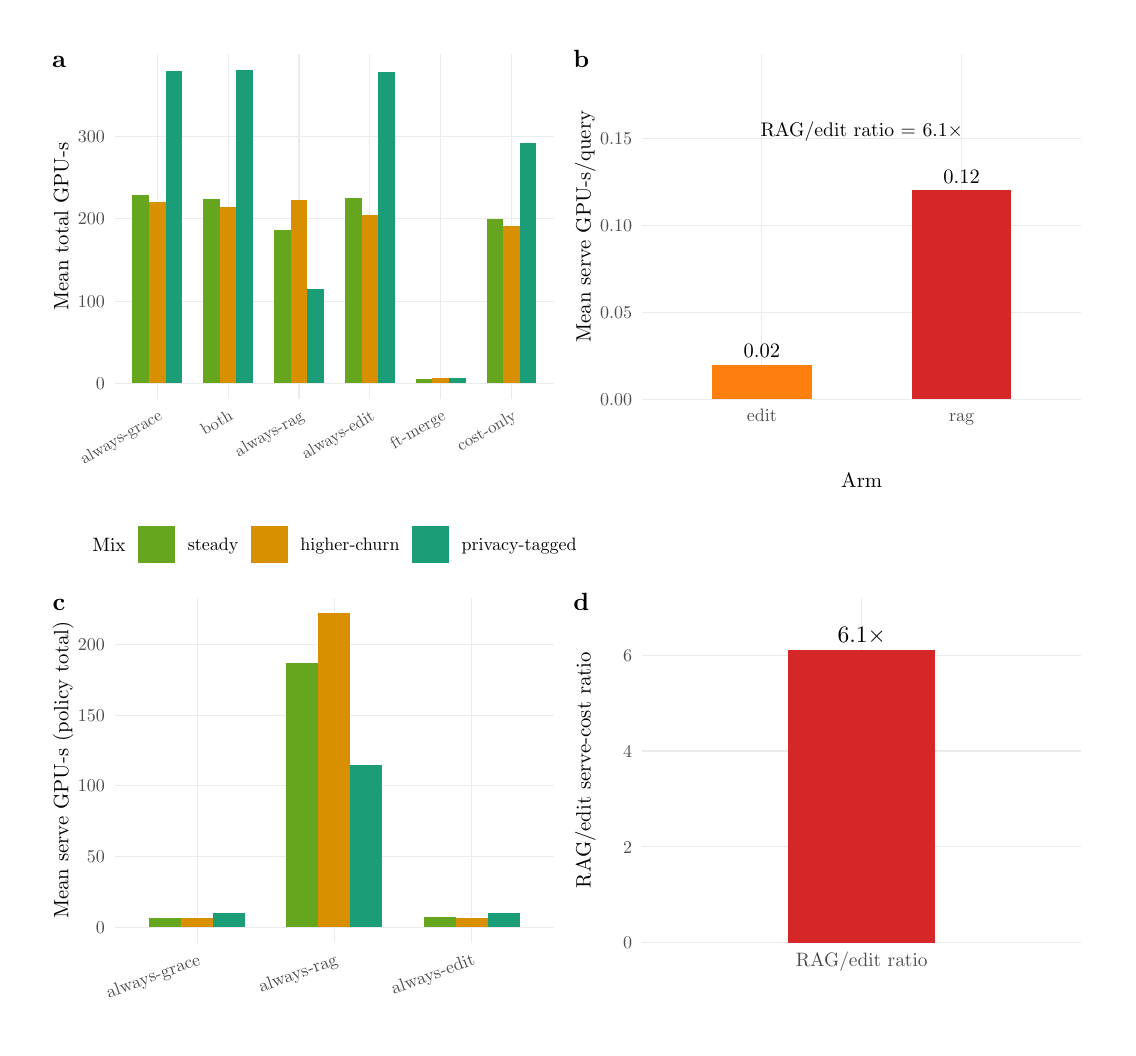
\begin{tikzpicture}[x=1pt,y=1pt]
\definecolor{fillColor}{RGB}{255,255,255}
\path[use as bounding box,fill=fillColor,fill opacity=0.00] (0,0) rectangle (390.26,361.35);
\begin{scope}
\path[clip] (  0.00,  0.00) rectangle (390.26,361.35);
\definecolor{drawColor}{RGB}{255,255,255}
\definecolor{fillColor}{RGB}{255,255,255}

\path[draw=drawColor,line width= 0.6pt,line join=round,line cap=round,fill=fillColor] (  0.00,  0.00) rectangle (390.26,361.35);
\end{scope}
\begin{scope}
\path[clip] (  5.50,159.41) rectangle (194.23,355.85);
\definecolor{fillColor}{RGB}{255,255,255}

\path[fill=fillColor] (  5.50,159.41) rectangle (194.23,355.85);
\end{scope}
\begin{scope}
\path[clip] (194.23,159.41) rectangle (384.76,355.85);
\definecolor{fillColor}{RGB}{255,255,255}

\path[fill=fillColor] (194.23,159.41) rectangle (384.76,355.85);
\end{scope}
\begin{scope}
\path[clip] (  5.50,  5.50) rectangle (194.23,159.41);
\definecolor{fillColor}{RGB}{255,255,255}

\path[fill=fillColor] (  5.50,  5.50) rectangle (194.23,159.41);
\end{scope}
\begin{scope}
\path[clip] (194.23,  5.50) rectangle (384.76,159.41);
\definecolor{fillColor}{RGB}{255,255,255}

\path[fill=fillColor] (194.23,  5.50) rectangle (384.76,159.41);
\end{scope}
\begin{scope}
\path[clip] ( 31.47,227.11) rectangle (190.23,351.85);
\definecolor{drawColor}{gray}{0.92}

\path[draw=drawColor,line width= 0.4pt,line join=round] ( 31.47,232.78) --
	(190.23,232.78);

\path[draw=drawColor,line width= 0.4pt,line join=round] ( 31.47,262.56) --
	(190.23,262.56);

\path[draw=drawColor,line width= 0.4pt,line join=round] ( 31.47,292.34) --
	(190.23,292.34);

\path[draw=drawColor,line width= 0.4pt,line join=round] ( 31.47,322.11) --
	(190.23,322.11);

\path[draw=drawColor,line width= 0.4pt,line join=round] ( 46.83,227.11) --
	( 46.83,351.85);

\path[draw=drawColor,line width= 0.4pt,line join=round] ( 72.44,227.11) --
	( 72.44,351.85);

\path[draw=drawColor,line width= 0.4pt,line join=round] ( 98.05,227.11) --
	( 98.05,351.85);

\path[draw=drawColor,line width= 0.4pt,line join=round] (123.65,227.11) --
	(123.65,351.85);

\path[draw=drawColor,line width= 0.4pt,line join=round] (149.26,227.11) --
	(149.26,351.85);

\path[draw=drawColor,line width= 0.4pt,line join=round] (174.86,227.11) --
	(174.86,351.85);
\definecolor{fillColor}{RGB}{102,166,31}

\path[fill=fillColor] ( 37.87,232.78) rectangle ( 43.85,300.98);

\path[fill=fillColor] ( 63.48,232.78) rectangle ( 69.45,299.51);

\path[fill=fillColor] ( 89.08,232.78) rectangle ( 95.06,288.34);

\path[fill=fillColor] (114.69,232.78) rectangle (120.66,299.91);

\path[fill=fillColor] (140.30,232.78) rectangle (146.27,234.54);

\path[fill=fillColor] (165.90,232.78) rectangle (171.88,292.24);
\definecolor{fillColor}{RGB}{216,144,0}

\path[fill=fillColor] ( 43.85,232.78) rectangle ( 49.82,298.29);

\path[fill=fillColor] ( 69.45,232.78) rectangle ( 75.43,296.61);

\path[fill=fillColor] ( 95.06,232.78) rectangle (101.03,298.91);

\path[fill=fillColor] (120.66,232.78) rectangle (126.64,293.78);

\path[fill=fillColor] (146.27,232.78) rectangle (152.24,234.76);

\path[fill=fillColor] (171.88,232.78) rectangle (177.85,289.81);
\definecolor{fillColor}{RGB}{27,158,119}

\path[fill=fillColor] ( 49.82,232.78) rectangle ( 55.80,345.52);

\path[fill=fillColor] ( 75.43,232.78) rectangle ( 81.40,346.18);

\path[fill=fillColor] (101.03,232.78) rectangle (107.01,266.87);

\path[fill=fillColor] (126.64,232.78) rectangle (132.61,345.31);

\path[fill=fillColor] (152.24,232.78) rectangle (158.22,234.69);

\path[fill=fillColor] (177.85,232.78) rectangle (183.83,319.76);
\end{scope}
\begin{scope}
\path[clip] (  0.00,  0.00) rectangle (390.26,361.35);
\definecolor{drawColor}{gray}{0.30}

\node[text=drawColor,anchor=base east,inner sep=0pt, outer sep=0pt, scale=  0.65] at ( 27.87,230.55) {0};

\node[text=drawColor,anchor=base east,inner sep=0pt, outer sep=0pt, scale=  0.65] at ( 27.87,260.32) {100};

\node[text=drawColor,anchor=base east,inner sep=0pt, outer sep=0pt, scale=  0.65] at ( 27.87,290.10) {200};

\node[text=drawColor,anchor=base east,inner sep=0pt, outer sep=0pt, scale=  0.65] at ( 27.87,319.87) {300};
\end{scope}
\begin{scope}
\path[clip] (  0.00,  0.00) rectangle (390.26,361.35);
\definecolor{drawColor}{gray}{0.30}

\node[text=drawColor,rotate= 30.00,anchor=base east,inner sep=0pt, outer sep=0pt, scale=  0.60] at ( 48.90,219.94) {always-grace};

\node[text=drawColor,rotate= 30.00,anchor=base east,inner sep=0pt, outer sep=0pt, scale=  0.60] at ( 74.51,219.94) {both};

\node[text=drawColor,rotate= 30.00,anchor=base east,inner sep=0pt, outer sep=0pt, scale=  0.60] at (100.11,219.94) {always-rag};

\node[text=drawColor,rotate= 30.00,anchor=base east,inner sep=0pt, outer sep=0pt, scale=  0.60] at (125.72,219.94) {always-edit};

\node[text=drawColor,rotate= 30.00,anchor=base east,inner sep=0pt, outer sep=0pt, scale=  0.60] at (151.32,219.94) {ft-merge};

\node[text=drawColor,rotate= 30.00,anchor=base east,inner sep=0pt, outer sep=0pt, scale=  0.60] at (176.93,219.94) {cost-only};
\end{scope}
\begin{scope}
\path[clip] (  0.00,  0.00) rectangle (390.26,361.35);
\definecolor{drawColor}{RGB}{0,0,0}

\node[text=drawColor,rotate= 90.00,anchor=base,inner sep=0pt, outer sep=0pt, scale=  0.75] at ( 14.67,289.48) {Mean total GPU-s};
\end{scope}
\begin{scope}
\path[clip] (  0.00,  0.00) rectangle (390.26,361.35);
\definecolor{drawColor}{RGB}{0,0,0}

\node[text=drawColor,anchor=base west,inner sep=0pt, outer sep=0pt, scale=  0.70] at ( 23.35,172.23) {Mix};
\end{scope}
\begin{scope}
\path[clip] (  0.00,  0.00) rectangle (390.26,361.35);
\definecolor{fillColor}{RGB}{102,166,31}

\path[fill=fillColor] ( 39.92,167.93) rectangle ( 53.34,181.35);
\end{scope}
\begin{scope}
\path[clip] (  0.00,  0.00) rectangle (390.26,361.35);
\definecolor{fillColor}{RGB}{216,144,0}

\path[fill=fillColor] ( 80.64,167.93) rectangle ( 94.06,181.35);
\end{scope}
\begin{scope}
\path[clip] (  0.00,  0.00) rectangle (390.26,361.35);
\definecolor{fillColor}{RGB}{27,158,119}

\path[fill=fillColor] (138.87,167.93) rectangle (152.29,181.35);
\end{scope}
\begin{scope}
\path[clip] (  0.00,  0.00) rectangle (390.26,361.35);
\definecolor{drawColor}{RGB}{0,0,0}

\node[text=drawColor,anchor=base west,inner sep=0pt, outer sep=0pt, scale=  0.65] at ( 57.86,172.40) {steady};
\end{scope}
\begin{scope}
\path[clip] (  0.00,  0.00) rectangle (390.26,361.35);
\definecolor{drawColor}{RGB}{0,0,0}

\node[text=drawColor,anchor=base west,inner sep=0pt, outer sep=0pt, scale=  0.65] at ( 98.58,172.40) {higher-churn};
\end{scope}
\begin{scope}
\path[clip] (  0.00,  0.00) rectangle (390.26,361.35);
\definecolor{drawColor}{RGB}{0,0,0}

\node[text=drawColor,anchor=base west,inner sep=0pt, outer sep=0pt, scale=  0.65] at (156.81,172.40) {privacy-tagged};
\end{scope}
\begin{scope}
\path[clip] (  0.00,  0.00) rectangle (390.26,361.35);
\definecolor{drawColor}{RGB}{0,0,0}

\node[text=drawColor,anchor=base,inner sep=0pt, outer sep=0pt, scale=  0.90] at ( 11.31,346.86) {\bfseries a};
\end{scope}
\begin{scope}
\path[clip] (222.00,227.11) rectangle (380.76,351.85);
\definecolor{drawColor}{gray}{0.92}

\path[draw=drawColor,line width= 0.4pt,line join=round] (222.00,227.11) --
	(380.76,227.11);

\path[draw=drawColor,line width= 0.4pt,line join=round] (222.00,258.55) --
	(380.76,258.55);

\path[draw=drawColor,line width= 0.4pt,line join=round] (222.00,289.99) --
	(380.76,289.99);

\path[draw=drawColor,line width= 0.4pt,line join=round] (222.00,321.42) --
	(380.76,321.42);

\path[draw=drawColor,line width= 0.4pt,line join=round] (265.30,227.11) --
	(265.30,351.85);

\path[draw=drawColor,line width= 0.4pt,line join=round] (337.46,227.11) --
	(337.46,351.85);
\definecolor{fillColor}{RGB}{255,127,14}

\path[fill=fillColor] (247.26,227.11) rectangle (283.34,239.49);
\definecolor{fillColor}{RGB}{214,39,40}

\path[fill=fillColor] (319.42,227.11) rectangle (355.50,302.61);
\definecolor{drawColor}{RGB}{0,0,0}

\node[text=drawColor,anchor=base,inner sep=0pt, outer sep=0pt, scale=  0.74] at (265.30,242.04) {0.02};

\node[text=drawColor,anchor=base,inner sep=0pt, outer sep=0pt, scale=  0.74] at (337.46,305.16) {0.12};

\node[text=drawColor,anchor=base,inner sep=0pt, outer sep=0pt, scale=  0.71] at (301.38,322.11) {RAG/edit ratio = 6.1$\times$};
\end{scope}
\begin{scope}
\path[clip] (  0.00,  0.00) rectangle (390.26,361.35);
\definecolor{drawColor}{gray}{0.30}

\node[text=drawColor,anchor=base east,inner sep=0pt, outer sep=0pt, scale=  0.65] at (218.40,224.88) {0.00};

\node[text=drawColor,anchor=base east,inner sep=0pt, outer sep=0pt, scale=  0.65] at (218.40,256.31) {0.05};

\node[text=drawColor,anchor=base east,inner sep=0pt, outer sep=0pt, scale=  0.65] at (218.40,287.75) {0.10};

\node[text=drawColor,anchor=base east,inner sep=0pt, outer sep=0pt, scale=  0.65] at (218.40,319.18) {0.15};
\end{scope}
\begin{scope}
\path[clip] (  0.00,  0.00) rectangle (390.26,361.35);
\definecolor{drawColor}{gray}{0.30}

\node[text=drawColor,anchor=base,inner sep=0pt, outer sep=0pt, scale=  0.65] at (265.30,219.04) {edit};

\node[text=drawColor,anchor=base,inner sep=0pt, outer sep=0pt, scale=  0.65] at (337.46,219.04) {rag};
\end{scope}
\begin{scope}
\path[clip] (  0.00,  0.00) rectangle (390.26,361.35);
\definecolor{drawColor}{RGB}{0,0,0}

\node[text=drawColor,anchor=base,inner sep=0pt, outer sep=0pt, scale=  0.75] at (301.38,195.32) {Arm};
\end{scope}
\begin{scope}
\path[clip] (  0.00,  0.00) rectangle (390.26,361.35);
\definecolor{drawColor}{RGB}{0,0,0}

\node[text=drawColor,rotate= 90.00,anchor=base,inner sep=0pt, outer sep=0pt, scale=  0.75] at (203.39,289.48) {Mean serve GPU-s/query};
\end{scope}
\begin{scope}
\path[clip] (  0.00,  0.00) rectangle (390.26,361.35);
\definecolor{drawColor}{RGB}{0,0,0}

\node[text=drawColor,anchor=base,inner sep=0pt, outer sep=0pt, scale=  0.90] at (200.05,346.86) {\bfseries b};
\end{scope}
\begin{scope}
\path[clip] ( 31.47, 30.67) rectangle (190.23,155.41);
\definecolor{drawColor}{gray}{0.92}

\path[draw=drawColor,line width= 0.4pt,line join=round] ( 31.47, 36.34) --
	(190.23, 36.34);

\path[draw=drawColor,line width= 0.4pt,line join=round] ( 31.47, 61.88) --
	(190.23, 61.88);

\path[draw=drawColor,line width= 0.4pt,line join=round] ( 31.47, 87.41) --
	(190.23, 87.41);

\path[draw=drawColor,line width= 0.4pt,line join=round] ( 31.47,112.94) --
	(190.23,112.94);

\path[draw=drawColor,line width= 0.4pt,line join=round] ( 31.47,138.47) --
	(190.23,138.47);

\path[draw=drawColor,line width= 0.4pt,line join=round] ( 61.24, 30.67) --
	( 61.24,155.41);

\path[draw=drawColor,line width= 0.4pt,line join=round] (110.85, 30.67) --
	(110.85,155.41);

\path[draw=drawColor,line width= 0.4pt,line join=round] (160.46, 30.67) --
	(160.46,155.41);
\definecolor{fillColor}{RGB}{102,166,31}

\path[fill=fillColor] ( 43.87, 36.34) rectangle ( 55.45, 39.71);

\path[fill=fillColor] ( 93.48, 36.34) rectangle (105.06,131.62);

\path[fill=fillColor] (143.10, 36.34) rectangle (154.67, 39.90);
\definecolor{fillColor}{RGB}{216,144,0}

\path[fill=fillColor] ( 55.45, 36.34) rectangle ( 67.03, 39.59);

\path[fill=fillColor] (105.06, 36.34) rectangle (116.64,149.74);

\path[fill=fillColor] (154.67, 36.34) rectangle (166.25, 39.80);
\definecolor{fillColor}{RGB}{27,158,119}

\path[fill=fillColor] ( 67.03, 36.34) rectangle ( 78.60, 41.54);

\path[fill=fillColor] (116.64, 36.34) rectangle (128.21, 94.79);

\path[fill=fillColor] (166.25, 36.34) rectangle (177.82, 41.35);
\end{scope}
\begin{scope}
\path[clip] (  0.00,  0.00) rectangle (390.26,361.35);
\definecolor{drawColor}{gray}{0.30}

\node[text=drawColor,anchor=base east,inner sep=0pt, outer sep=0pt, scale=  0.65] at ( 27.87, 34.11) {0};

\node[text=drawColor,anchor=base east,inner sep=0pt, outer sep=0pt, scale=  0.65] at ( 27.87, 59.64) {50};

\node[text=drawColor,anchor=base east,inner sep=0pt, outer sep=0pt, scale=  0.65] at ( 27.87, 85.17) {100};

\node[text=drawColor,anchor=base east,inner sep=0pt, outer sep=0pt, scale=  0.65] at ( 27.87,110.70) {150};

\node[text=drawColor,anchor=base east,inner sep=0pt, outer sep=0pt, scale=  0.65] at ( 27.87,136.24) {200};
\end{scope}
\begin{scope}
\path[clip] (  0.00,  0.00) rectangle (390.26,361.35);
\definecolor{drawColor}{gray}{0.30}

\node[text=drawColor,rotate= 20.00,anchor=base east,inner sep=0pt, outer sep=0pt, scale=  0.65] at ( 62.77, 22.87) {always-grace};

\node[text=drawColor,rotate= 20.00,anchor=base east,inner sep=0pt, outer sep=0pt, scale=  0.65] at (112.38, 22.87) {always-rag};

\node[text=drawColor,rotate= 20.00,anchor=base east,inner sep=0pt, outer sep=0pt, scale=  0.65] at (161.99, 22.87) {always-edit};
\end{scope}
\begin{scope}
\path[clip] (  0.00,  0.00) rectangle (390.26,361.35);
\definecolor{drawColor}{RGB}{0,0,0}

\node[text=drawColor,rotate= 90.00,anchor=base,inner sep=0pt, outer sep=0pt, scale=  0.75] at ( 14.67, 93.04) {Mean serve GPU-s (policy total)};
\end{scope}
\begin{scope}
\path[clip] (  0.00,  0.00) rectangle (390.26,361.35);
\definecolor{drawColor}{RGB}{0,0,0}

\node[text=drawColor,anchor=base,inner sep=0pt, outer sep=0pt, scale=  0.90] at ( 11.31,150.85) {\bfseries c};
\end{scope}
\begin{scope}
\path[clip] (222.00, 30.67) rectangle (380.76,155.41);
\definecolor{drawColor}{gray}{0.92}

\path[draw=drawColor,line width= 0.4pt,line join=round] (222.00, 30.67) --
	(380.76, 30.67);

\path[draw=drawColor,line width= 0.4pt,line join=round] (222.00, 65.32) --
	(380.76, 65.32);

\path[draw=drawColor,line width= 0.4pt,line join=round] (222.00, 99.97) --
	(380.76, 99.97);

\path[draw=drawColor,line width= 0.4pt,line join=round] (222.00,134.62) --
	(380.76,134.62);

\path[draw=drawColor,line width= 0.4pt,line join=round] (301.38, 30.67) --
	(301.38,155.41);
\definecolor{fillColor}{RGB}{214,39,40}

\path[fill=fillColor] (274.92, 30.67) rectangle (327.84,136.38);
\definecolor{drawColor}{RGB}{0,0,0}

\node[text=drawColor,anchor=base,inner sep=0pt, outer sep=0pt, scale=  0.85] at (301.38,139.32) {6.1$\times$};
\end{scope}
\begin{scope}
\path[clip] (  0.00,  0.00) rectangle (390.26,361.35);
\definecolor{drawColor}{gray}{0.30}

\node[text=drawColor,anchor=base east,inner sep=0pt, outer sep=0pt, scale=  0.65] at (218.40, 28.44) {0};

\node[text=drawColor,anchor=base east,inner sep=0pt, outer sep=0pt, scale=  0.65] at (218.40, 63.09) {2};

\node[text=drawColor,anchor=base east,inner sep=0pt, outer sep=0pt, scale=  0.65] at (218.40, 97.73) {4};

\node[text=drawColor,anchor=base east,inner sep=0pt, outer sep=0pt, scale=  0.65] at (218.40,132.38) {6};
\end{scope}
\begin{scope}
\path[clip] (  0.00,  0.00) rectangle (390.26,361.35);
\definecolor{drawColor}{gray}{0.30}

\node[text=drawColor,anchor=base,inner sep=0pt, outer sep=0pt, scale=  0.70] at (301.38, 22.25) {RAG/edit ratio};
\end{scope}
\begin{scope}
\path[clip] (  0.00,  0.00) rectangle (390.26,361.35);
\definecolor{drawColor}{RGB}{0,0,0}

\node[text=drawColor,rotate= 90.00,anchor=base,inner sep=0pt, outer sep=0pt, scale=  0.75] at (203.39, 93.04) {RAG/edit serve-cost ratio};
\end{scope}
\begin{scope}
\path[clip] (  0.00,  0.00) rectangle (390.26,361.35);
\definecolor{drawColor}{RGB}{0,0,0}

\node[text=drawColor,anchor=base,inner sep=0pt, outer sep=0pt, scale=  0.90] at (200.05,150.85) {\bfseries d};
\end{scope}
\end{tikzpicture}

\caption{RAG cost surprise visualization. Panel annotation: measured RAG/edit
serve ratio $=6.1\times$ on the measured-store slice. Against the frozen synthetic
anchor the same contrast is $\approx$17$\times$ (Table~\ref{tab:costratio}); the
anchor under-estimated the gap by an order of magnitude.}
\label{fig:ragcost-app}
\end{figure}

\begin{figure}[!ht]
\centering
% SOURCE: ../../edit-harness/results/frame_a/cells/cell_*_real_MIX_A_*.json
% !TEX encoding = UTF-8 Unicode
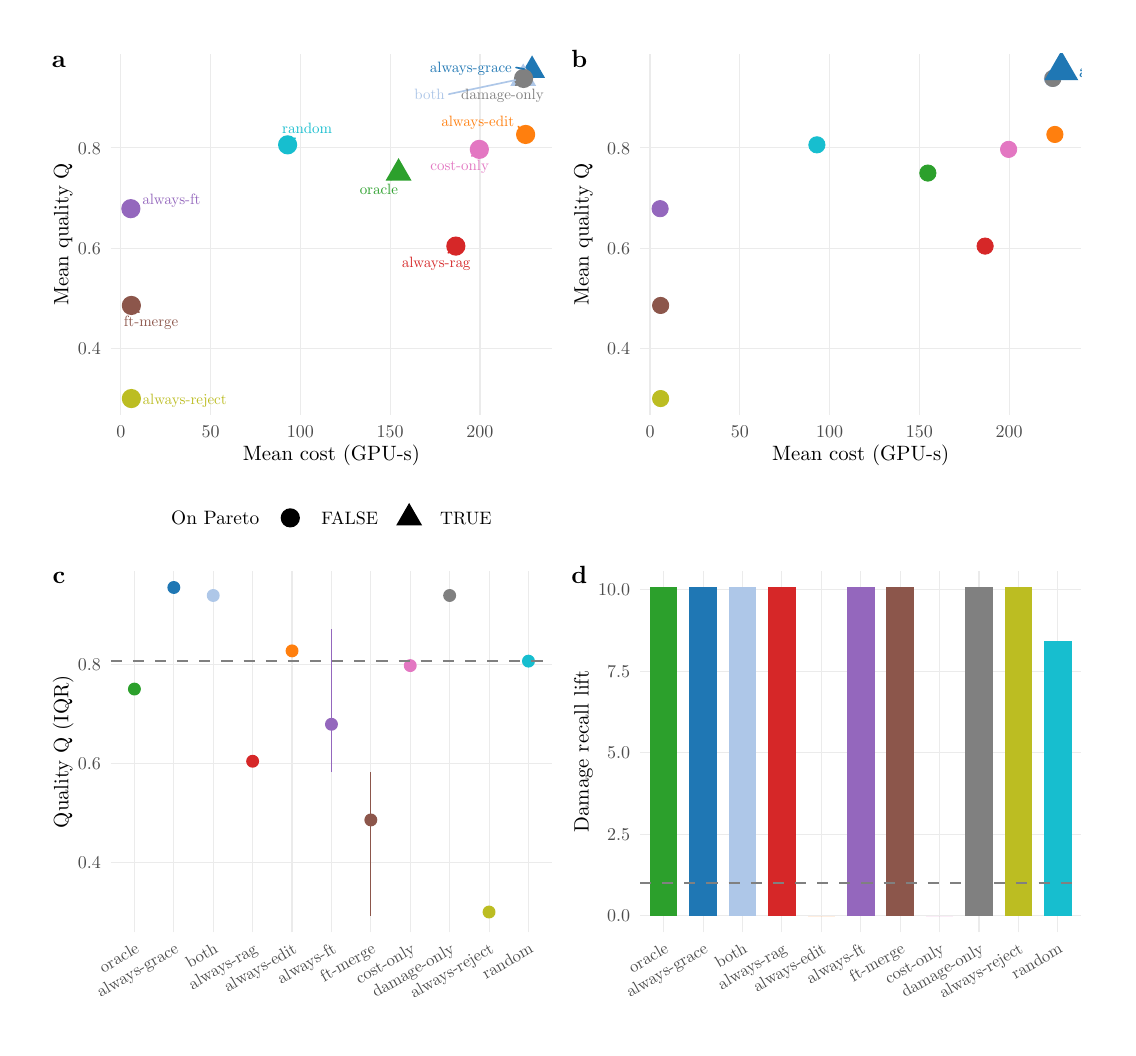
\begin{tikzpicture}[x=1pt,y=1pt]
\definecolor{fillColor}{RGB}{255,255,255}
\path[use as bounding box,fill=fillColor,fill opacity=0.00] (0,0) rectangle (390.26,361.35);
\begin{scope}
\path[clip] (  0.00,  0.00) rectangle (390.26,361.35);
\definecolor{drawColor}{RGB}{255,255,255}
\definecolor{fillColor}{RGB}{255,255,255}

\path[draw=drawColor,line width= 0.6pt,line join=round,line cap=round,fill=fillColor] (  0.00,  0.00) rectangle (390.26,361.35);
\end{scope}
\begin{scope}
\path[clip] (  5.50,168.99) rectangle (193.50,355.85);
\definecolor{fillColor}{RGB}{255,255,255}

\path[fill=fillColor] (  5.50,168.99) rectangle (193.50,355.85);
\end{scope}
\begin{scope}
\path[clip] (193.50,168.99) rectangle (384.76,355.85);
\definecolor{fillColor}{RGB}{255,255,255}

\path[fill=fillColor] (193.50,168.99) rectangle (384.76,355.85);
\end{scope}
\begin{scope}
\path[clip] (  5.50,  5.50) rectangle (193.50,168.99);
\definecolor{fillColor}{RGB}{255,255,255}

\path[fill=fillColor] (  5.50,  5.50) rectangle (193.50,168.99);
\end{scope}
\begin{scope}
\path[clip] (193.50,  5.50) rectangle (384.76,168.99);
\definecolor{fillColor}{RGB}{255,255,255}

\path[fill=fillColor] (193.50,  5.50) rectangle (384.76,168.99);
\end{scope}
\begin{scope}
\path[clip] ( 30.03,221.41) rectangle (189.50,351.85);
\definecolor{drawColor}{gray}{0.92}

\path[draw=drawColor,line width= 0.4pt,line join=round] ( 30.03,245.46) --
	(189.50,245.46);

\path[draw=drawColor,line width= 0.4pt,line join=round] ( 30.03,281.70) --
	(189.50,281.70);

\path[draw=drawColor,line width= 0.4pt,line join=round] ( 30.03,317.94) --
	(189.50,317.94);

\path[draw=drawColor,line width= 0.4pt,line join=round] ( 33.64,221.41) --
	( 33.64,351.85);

\path[draw=drawColor,line width= 0.4pt,line join=round] ( 66.09,221.41) --
	( 66.09,351.85);

\path[draw=drawColor,line width= 0.4pt,line join=round] ( 98.53,221.41) --
	( 98.53,351.85);

\path[draw=drawColor,line width= 0.4pt,line join=round] (130.98,221.41) --
	(130.98,351.85);

\path[draw=drawColor,line width= 0.4pt,line join=round] (163.43,221.41) --
	(163.43,351.85);
\definecolor{fillColor}{RGB}{44,160,44}

\path[fill=fillColor] (134.02,314.21) --
	(138.70,306.11) --
	(129.35,306.11) --
	cycle;
\definecolor{fillColor}{RGB}{31,119,180}

\path[fill=fillColor] (182.26,351.32) --
	(186.93,343.22) --
	(177.58,343.22) --
	cycle;
\definecolor{fillColor}{RGB}{174,199,232}

\path[fill=fillColor] (179.05,348.40) --
	(183.73,340.30) --
	(174.38,340.30) --
	cycle;
\definecolor{fillColor}{RGB}{214,39,40}

\path[fill=fillColor] (154.72,282.42) circle (  3.47);
\definecolor{fillColor}{RGB}{255,127,14}

\path[fill=fillColor] (179.93,322.76) circle (  3.47);
\definecolor{fillColor}{RGB}{148,103,189}

\path[fill=fillColor] ( 37.28,295.94) circle (  3.47);
\definecolor{fillColor}{RGB}{140,86,75}

\path[fill=fillColor] ( 37.47,260.97) circle (  3.47);
\definecolor{fillColor}{RGB}{227,119,194}

\path[fill=fillColor] (163.21,317.37) circle (  3.47);
\definecolor{fillColor}{gray}{0.50}

\path[fill=fillColor] (179.19,343.00) circle (  3.47);
\definecolor{fillColor}{RGB}{188,189,34}

\path[fill=fillColor] ( 37.47,227.33) circle (  3.47);
\definecolor{fillColor}{RGB}{23,190,207}

\path[fill=fillColor] ( 93.93,319.01) circle (  3.47);
\definecolor{drawColor}{RGB}{44,160,44}

\path[draw=drawColor,line width= 0.6pt,line join=round,line cap=round] (131.26,306.36) -- (131.87,306.90);
\definecolor{drawColor}{RGB}{31,119,180}

\path[draw=drawColor,line width= 0.6pt,line join=round,line cap=round] (176.46,346.95) -- (179.42,346.42);
\definecolor{drawColor}{RGB}{174,199,232}

\path[draw=drawColor,line width= 0.6pt,line join=round,line cap=round] (152.17,337.32) -- (176.24,342.40);
\definecolor{drawColor}{RGB}{214,39,40}

\path[draw=drawColor,line width= 0.6pt,line join=round,line cap=round] (151.94,279.96) -- (152.56,280.51);
\definecolor{drawColor}{RGB}{255,127,14}

\path[draw=drawColor,line width= 0.6pt,line join=round,line cap=round] (177.29,325.65) -- (177.99,324.88);
\definecolor{drawColor}{RGB}{148,103,189}

\path[draw=drawColor,line width= 0.6pt,line join=round,line cap=round] ( 39.91,297.80) -- ( 39.63,297.60);
\definecolor{drawColor}{RGB}{140,86,75}

\path[draw=drawColor,line width= 0.6pt,line join=round,line cap=round] ( 40.25,258.50) -- ( 39.62,259.06);
\definecolor{drawColor}{RGB}{227,119,194}

\path[draw=drawColor,line width= 0.6pt,line join=round,line cap=round] (160.46,314.94) -- (161.06,315.46);
\definecolor{drawColor}{gray}{0.50}

\path[draw=drawColor,line width= 0.6pt,line join=round,line cap=round] (176.37,340.52) -- (177.03,341.10);
\definecolor{drawColor}{RGB}{23,190,207}

\path[draw=drawColor,line width= 0.6pt,line join=round,line cap=round] ( 96.66,321.44) -- ( 96.08,320.92);
\definecolor{drawColor}{RGB}{44,160,44}

\node[text=drawColor,anchor=base,inner sep=0pt, outer sep=0pt, scale=  0.54] at (126.91,301.13) {oracle};
\definecolor{drawColor}{RGB}{31,119,180}

\node[text=drawColor,anchor=base,inner sep=0pt, outer sep=0pt, scale=  0.54] at (160.14,345.12) {always-grace};
\definecolor{drawColor}{RGB}{174,199,232}

\node[text=drawColor,anchor=base,inner sep=0pt, outer sep=0pt, scale=  0.54] at (145.19,335.37) {both};
\definecolor{drawColor}{RGB}{214,39,40}

\node[text=drawColor,anchor=base,inner sep=0pt, outer sep=0pt, scale=  0.54] at (147.60,274.73) {always-rag};
\definecolor{drawColor}{RGB}{255,127,14}

\node[text=drawColor,anchor=base,inner sep=0pt, outer sep=0pt, scale=  0.54] at (162.63,325.51) {always-edit};
\definecolor{drawColor}{RGB}{148,103,189}

\node[text=drawColor,anchor=base,inner sep=0pt, outer sep=0pt, scale=  0.54] at ( 51.94,297.51) {always-ft};
\definecolor{drawColor}{RGB}{140,86,75}

\node[text=drawColor,anchor=base,inner sep=0pt, outer sep=0pt, scale=  0.54] at ( 44.61,253.27) {ft-merge};
\definecolor{drawColor}{RGB}{227,119,194}

\node[text=drawColor,anchor=base,inner sep=0pt, outer sep=0pt, scale=  0.54] at (156.12,309.71) {cost-only};
\definecolor{drawColor}{gray}{0.50}

\node[text=drawColor,anchor=base,inner sep=0pt, outer sep=0pt, scale=  0.54] at (171.56,335.29) {damage-only};
\definecolor{drawColor}{RGB}{188,189,34}

\node[text=drawColor,anchor=base,inner sep=0pt, outer sep=0pt, scale=  0.54] at ( 56.74,225.27) {always-reject};
\definecolor{drawColor}{RGB}{23,190,207}

\node[text=drawColor,anchor=base,inner sep=0pt, outer sep=0pt, scale=  0.54] at (100.99,322.94) {random};
\end{scope}
\begin{scope}
\path[clip] (  0.00,  0.00) rectangle (390.26,361.35);
\definecolor{drawColor}{gray}{0.30}

\node[text=drawColor,anchor=base east,inner sep=0pt, outer sep=0pt, scale=  0.65] at ( 26.43,243.22) {0.4};

\node[text=drawColor,anchor=base east,inner sep=0pt, outer sep=0pt, scale=  0.65] at ( 26.43,279.46) {0.6};

\node[text=drawColor,anchor=base east,inner sep=0pt, outer sep=0pt, scale=  0.65] at ( 26.43,315.70) {0.8};
\end{scope}
\begin{scope}
\path[clip] (  0.00,  0.00) rectangle (390.26,361.35);
\definecolor{drawColor}{gray}{0.30}

\node[text=drawColor,anchor=base,inner sep=0pt, outer sep=0pt, scale=  0.65] at ( 33.64,213.33) {0};

\node[text=drawColor,anchor=base,inner sep=0pt, outer sep=0pt, scale=  0.65] at ( 66.09,213.33) {50};

\node[text=drawColor,anchor=base,inner sep=0pt, outer sep=0pt, scale=  0.65] at ( 98.53,213.33) {100};

\node[text=drawColor,anchor=base,inner sep=0pt, outer sep=0pt, scale=  0.65] at (130.98,213.33) {150};

\node[text=drawColor,anchor=base,inner sep=0pt, outer sep=0pt, scale=  0.65] at (163.43,213.33) {200};
\end{scope}
\begin{scope}
\path[clip] (  0.00,  0.00) rectangle (390.26,361.35);
\definecolor{drawColor}{RGB}{0,0,0}

\node[text=drawColor,anchor=base,inner sep=0pt, outer sep=0pt, scale=  0.75] at (109.77,204.90) {Mean cost (GPU-s)};
\end{scope}
\begin{scope}
\path[clip] (  0.00,  0.00) rectangle (390.26,361.35);
\definecolor{drawColor}{RGB}{0,0,0}

\node[text=drawColor,rotate= 90.00,anchor=base,inner sep=0pt, outer sep=0pt, scale=  0.75] at ( 14.67,286.63) {Mean quality Q};
\end{scope}
\begin{scope}
\path[clip] (  0.00,  0.00) rectangle (390.26,361.35);
\definecolor{drawColor}{RGB}{0,0,0}

\node[text=drawColor,anchor=base west,inner sep=0pt, outer sep=0pt, scale=  0.70] at ( 51.87,181.80) {On Pareto};
\end{scope}
\begin{scope}
\path[clip] (  0.00,  0.00) rectangle (390.26,361.35);
\definecolor{fillColor}{RGB}{0,0,0}

\path[fill=fillColor] ( 94.90,184.21) circle (  3.47);
\end{scope}
\begin{scope}
\path[clip] (  0.00,  0.00) rectangle (390.26,361.35);
\definecolor{fillColor}{RGB}{0,0,0}

\path[fill=fillColor] (137.84,189.61) --
	(142.52,181.52) --
	(133.17,181.52) --
	cycle;
\end{scope}
\begin{scope}
\path[clip] (  0.00,  0.00) rectangle (390.26,361.35);
\definecolor{drawColor}{RGB}{0,0,0}

\node[text=drawColor,anchor=base west,inner sep=0pt, outer sep=0pt, scale=  0.65] at (106.13,181.98) {FALSE};
\end{scope}
\begin{scope}
\path[clip] (  0.00,  0.00) rectangle (390.26,361.35);
\definecolor{drawColor}{RGB}{0,0,0}

\node[text=drawColor,anchor=base west,inner sep=0pt, outer sep=0pt, scale=  0.65] at (149.07,181.98) {TRUE};
\end{scope}
\begin{scope}
\path[clip] (  0.00,  0.00) rectangle (390.26,361.35);
\definecolor{drawColor}{RGB}{0,0,0}

\node[text=drawColor,anchor=base,inner sep=0pt, outer sep=0pt, scale=  0.90] at ( 11.30,346.96) {\bfseries a};
\end{scope}
\begin{scope}
\path[clip] (221.28,221.41) rectangle (380.76,351.85);
\definecolor{drawColor}{gray}{0.92}

\path[draw=drawColor,line width= 0.4pt,line join=round] (221.28,245.46) --
	(380.76,245.46);

\path[draw=drawColor,line width= 0.4pt,line join=round] (221.28,281.70) --
	(380.76,281.70);

\path[draw=drawColor,line width= 0.4pt,line join=round] (221.28,317.94) --
	(380.76,317.94);

\path[draw=drawColor,line width= 0.4pt,line join=round] (224.89,221.41) --
	(224.89,351.85);

\path[draw=drawColor,line width= 0.4pt,line join=round] (257.34,221.41) --
	(257.34,351.85);

\path[draw=drawColor,line width= 0.4pt,line join=round] (289.79,221.41) --
	(289.79,351.85);

\path[draw=drawColor,line width= 0.4pt,line join=round] (322.23,221.41) --
	(322.23,351.85);

\path[draw=drawColor,line width= 0.4pt,line join=round] (354.68,221.41) --
	(354.68,351.85);
\definecolor{drawColor}{RGB}{44,160,44}
\definecolor{fillColor}{RGB}{44,160,44}

\path[draw=drawColor,line width= 0.3pt,line join=round,line cap=round,fill=fillColor] (325.28,308.81) circle (  2.94);
\definecolor{drawColor}{RGB}{31,119,180}
\definecolor{fillColor}{RGB}{31,119,180}

\path[draw=drawColor,line width= 0.3pt,line join=round,line cap=round,fill=fillColor] (373.51,345.92) circle (  2.94);
\definecolor{drawColor}{RGB}{174,199,232}
\definecolor{fillColor}{RGB}{174,199,232}

\path[draw=drawColor,line width= 0.3pt,line join=round,line cap=round,fill=fillColor] (370.31,343.00) circle (  2.94);
\definecolor{drawColor}{RGB}{214,39,40}
\definecolor{fillColor}{RGB}{214,39,40}

\path[draw=drawColor,line width= 0.3pt,line join=round,line cap=round,fill=fillColor] (345.97,282.42) circle (  2.94);
\definecolor{drawColor}{RGB}{255,127,14}
\definecolor{fillColor}{RGB}{255,127,14}

\path[draw=drawColor,line width= 0.3pt,line join=round,line cap=round,fill=fillColor] (371.18,322.76) circle (  2.94);
\definecolor{drawColor}{RGB}{148,103,189}
\definecolor{fillColor}{RGB}{148,103,189}

\path[draw=drawColor,line width= 0.3pt,line join=round,line cap=round,fill=fillColor] (228.53,295.94) circle (  2.94);
\definecolor{drawColor}{RGB}{140,86,75}
\definecolor{fillColor}{RGB}{140,86,75}

\path[draw=drawColor,line width= 0.3pt,line join=round,line cap=round,fill=fillColor] (228.72,260.97) circle (  2.94);
\definecolor{drawColor}{RGB}{227,119,194}
\definecolor{fillColor}{RGB}{227,119,194}

\path[draw=drawColor,line width= 0.3pt,line join=round,line cap=round,fill=fillColor] (354.46,317.37) circle (  2.94);
\definecolor{drawColor}{gray}{0.50}
\definecolor{fillColor}{gray}{0.50}

\path[draw=drawColor,line width= 0.3pt,line join=round,line cap=round,fill=fillColor] (370.45,343.00) circle (  2.94);
\definecolor{drawColor}{RGB}{188,189,34}
\definecolor{fillColor}{RGB}{188,189,34}

\path[draw=drawColor,line width= 0.3pt,line join=round,line cap=round,fill=fillColor] (228.72,227.33) circle (  2.94);
\definecolor{drawColor}{RGB}{23,190,207}
\definecolor{fillColor}{RGB}{23,190,207}

\path[draw=drawColor,line width= 0.3pt,line join=round,line cap=round,fill=fillColor] (285.18,319.01) circle (  2.94);
\definecolor{fillColor}{RGB}{31,119,180}

\path[fill=fillColor] (373.51,352.98) --
	(379.63,342.39) --
	(367.39,342.39) --
	cycle;
\definecolor{drawColor}{RGB}{31,119,180}

\node[text=drawColor,anchor=base west,inner sep=0pt, outer sep=0pt, scale=  0.71] at (379.83,343.47) {always\_grace};
\end{scope}
\begin{scope}
\path[clip] (  0.00,  0.00) rectangle (390.26,361.35);
\definecolor{drawColor}{gray}{0.30}

\node[text=drawColor,anchor=base east,inner sep=0pt, outer sep=0pt, scale=  0.65] at (217.68,243.22) {0.4};

\node[text=drawColor,anchor=base east,inner sep=0pt, outer sep=0pt, scale=  0.65] at (217.68,279.46) {0.6};

\node[text=drawColor,anchor=base east,inner sep=0pt, outer sep=0pt, scale=  0.65] at (217.68,315.70) {0.8};
\end{scope}
\begin{scope}
\path[clip] (  0.00,  0.00) rectangle (390.26,361.35);
\definecolor{drawColor}{gray}{0.30}

\node[text=drawColor,anchor=base,inner sep=0pt, outer sep=0pt, scale=  0.65] at (224.89,213.33) {0};

\node[text=drawColor,anchor=base,inner sep=0pt, outer sep=0pt, scale=  0.65] at (257.34,213.33) {50};

\node[text=drawColor,anchor=base,inner sep=0pt, outer sep=0pt, scale=  0.65] at (289.79,213.33) {100};

\node[text=drawColor,anchor=base,inner sep=0pt, outer sep=0pt, scale=  0.65] at (322.23,213.33) {150};

\node[text=drawColor,anchor=base,inner sep=0pt, outer sep=0pt, scale=  0.65] at (354.68,213.33) {200};
\end{scope}
\begin{scope}
\path[clip] (  0.00,  0.00) rectangle (390.26,361.35);
\definecolor{drawColor}{RGB}{0,0,0}

\node[text=drawColor,anchor=base,inner sep=0pt, outer sep=0pt, scale=  0.75] at (301.02,204.90) {Mean cost (GPU-s)};
\end{scope}
\begin{scope}
\path[clip] (  0.00,  0.00) rectangle (390.26,361.35);
\definecolor{drawColor}{RGB}{0,0,0}

\node[text=drawColor,rotate= 90.00,anchor=base,inner sep=0pt, outer sep=0pt, scale=  0.75] at (202.67,286.63) {Mean quality Q};
\end{scope}
\begin{scope}
\path[clip] (  0.00,  0.00) rectangle (390.26,361.35);
\definecolor{drawColor}{RGB}{0,0,0}

\node[text=drawColor,anchor=base,inner sep=0pt, outer sep=0pt, scale=  0.90] at (199.34,346.96) {\bfseries b};
\end{scope}
\begin{scope}
\path[clip] ( 30.03, 34.54) rectangle (189.50,164.99);
\definecolor{drawColor}{gray}{0.92}

\path[draw=drawColor,line width= 0.4pt,line join=round] ( 30.03, 59.71) --
	(189.50, 59.71);

\path[draw=drawColor,line width= 0.4pt,line join=round] ( 30.03, 95.55) --
	(189.50, 95.55);

\path[draw=drawColor,line width= 0.4pt,line join=round] ( 30.03,131.39) --
	(189.50,131.39);

\path[draw=drawColor,line width= 0.4pt,line join=round] ( 38.57, 34.54) --
	( 38.57,164.99);

\path[draw=drawColor,line width= 0.4pt,line join=round] ( 52.81, 34.54) --
	( 52.81,164.99);

\path[draw=drawColor,line width= 0.4pt,line join=round] ( 67.05, 34.54) --
	( 67.05,164.99);

\path[draw=drawColor,line width= 0.4pt,line join=round] ( 81.29, 34.54) --
	( 81.29,164.99);

\path[draw=drawColor,line width= 0.4pt,line join=round] ( 95.53, 34.54) --
	( 95.53,164.99);

\path[draw=drawColor,line width= 0.4pt,line join=round] (109.77, 34.54) --
	(109.77,164.99);

\path[draw=drawColor,line width= 0.4pt,line join=round] (124.00, 34.54) --
	(124.00,164.99);

\path[draw=drawColor,line width= 0.4pt,line join=round] (138.24, 34.54) --
	(138.24,164.99);

\path[draw=drawColor,line width= 0.4pt,line join=round] (152.48, 34.54) --
	(152.48,164.99);

\path[draw=drawColor,line width= 0.4pt,line join=round] (166.72, 34.54) --
	(166.72,164.99);

\path[draw=drawColor,line width= 0.4pt,line join=round] (180.96, 34.54) --
	(180.96,164.99);
\definecolor{drawColor}{RGB}{44,160,44}

\path[draw=drawColor,line width= 0.4pt,line join=round] ( 38.57,122.14) -- ( 38.57,122.57);
\definecolor{drawColor}{RGB}{31,119,180}

\path[draw=drawColor,line width= 0.4pt,line join=round] ( 52.81,159.06) -- ( 52.81,159.06);
\definecolor{drawColor}{RGB}{174,199,232}

\path[draw=drawColor,line width= 0.4pt,line join=round] ( 67.05,155.00) -- ( 67.05,158.40);
\definecolor{drawColor}{RGB}{214,39,40}

\path[draw=drawColor,line width= 0.4pt,line join=round] ( 81.29, 96.27) -- ( 81.29, 96.27);
\definecolor{drawColor}{RGB}{255,127,14}

\path[draw=drawColor,line width= 0.4pt,line join=round] ( 95.53,135.00) -- ( 95.53,137.88);
\definecolor{drawColor}{RGB}{148,103,189}

\path[draw=drawColor,line width= 0.4pt,line join=round] (109.77, 92.34) -- (109.77,144.22);
\definecolor{drawColor}{RGB}{140,86,75}

\path[draw=drawColor,line width= 0.4pt,line join=round] (124.00, 40.47) -- (124.00, 92.36);
\definecolor{drawColor}{RGB}{227,119,194}

\path[draw=drawColor,line width= 0.4pt,line join=round] (138.24,129.24) -- (138.24,132.62);
\definecolor{drawColor}{gray}{0.50}

\path[draw=drawColor,line width= 0.4pt,line join=round] (152.48,155.00) -- (152.48,158.40);
\definecolor{drawColor}{RGB}{188,189,34}

\path[draw=drawColor,line width= 0.4pt,line join=round] (166.72, 41.79) -- (166.72, 41.79);
\definecolor{drawColor}{RGB}{23,190,207}

\path[draw=drawColor,line width= 0.4pt,line join=round] (180.96,132.12) -- (180.96,133.00);
\definecolor{drawColor}{RGB}{44,160,44}
\definecolor{fillColor}{RGB}{44,160,44}

\path[draw=drawColor,line width= 0.5pt,line join=round,line cap=round,fill=fillColor] ( 38.57,122.36) circle (  2.08);
\definecolor{drawColor}{RGB}{31,119,180}
\definecolor{fillColor}{RGB}{31,119,180}

\path[draw=drawColor,line width= 0.5pt,line join=round,line cap=round,fill=fillColor] ( 52.81,159.06) circle (  2.08);
\definecolor{drawColor}{RGB}{174,199,232}
\definecolor{fillColor}{RGB}{174,199,232}

\path[draw=drawColor,line width= 0.5pt,line join=round,line cap=round,fill=fillColor] ( 67.05,156.17) circle (  2.08);
\definecolor{drawColor}{RGB}{214,39,40}
\definecolor{fillColor}{RGB}{214,39,40}

\path[draw=drawColor,line width= 0.5pt,line join=round,line cap=round,fill=fillColor] ( 81.29, 96.27) circle (  2.08);
\definecolor{drawColor}{RGB}{255,127,14}
\definecolor{fillColor}{RGB}{255,127,14}

\path[draw=drawColor,line width= 0.5pt,line join=round,line cap=round,fill=fillColor] ( 95.53,136.15) circle (  2.08);
\definecolor{drawColor}{RGB}{148,103,189}
\definecolor{fillColor}{RGB}{148,103,189}

\path[draw=drawColor,line width= 0.5pt,line join=round,line cap=round,fill=fillColor] (109.77,109.63) circle (  2.08);
\definecolor{drawColor}{RGB}{140,86,75}
\definecolor{fillColor}{RGB}{140,86,75}

\path[draw=drawColor,line width= 0.5pt,line join=round,line cap=round,fill=fillColor] (124.00, 75.06) circle (  2.08);
\definecolor{drawColor}{RGB}{227,119,194}
\definecolor{fillColor}{RGB}{227,119,194}

\path[draw=drawColor,line width= 0.5pt,line join=round,line cap=round,fill=fillColor] (138.24,130.83) circle (  2.08);
\definecolor{drawColor}{gray}{0.50}
\definecolor{fillColor}{gray}{0.50}

\path[draw=drawColor,line width= 0.5pt,line join=round,line cap=round,fill=fillColor] (152.48,156.17) circle (  2.08);
\definecolor{drawColor}{RGB}{188,189,34}
\definecolor{fillColor}{RGB}{188,189,34}

\path[draw=drawColor,line width= 0.5pt,line join=round,line cap=round,fill=fillColor] (166.72, 41.79) circle (  2.08);
\definecolor{drawColor}{RGB}{23,190,207}
\definecolor{fillColor}{RGB}{23,190,207}

\path[draw=drawColor,line width= 0.5pt,line join=round,line cap=round,fill=fillColor] (180.96,132.45) circle (  2.08);
\definecolor{drawColor}{gray}{0.50}

\path[draw=drawColor,line width= 0.5pt,dash pattern=on 4pt off 4pt ,line join=round] ( 30.03,132.45) -- (189.50,132.45);
\end{scope}
\begin{scope}
\path[clip] (  0.00,  0.00) rectangle (390.26,361.35);
\definecolor{drawColor}{gray}{0.30}

\node[text=drawColor,anchor=base east,inner sep=0pt, outer sep=0pt, scale=  0.65] at ( 26.43, 57.47) {0.4};

\node[text=drawColor,anchor=base east,inner sep=0pt, outer sep=0pt, scale=  0.65] at ( 26.43, 93.31) {0.6};

\node[text=drawColor,anchor=base east,inner sep=0pt, outer sep=0pt, scale=  0.65] at ( 26.43,129.15) {0.8};
\end{scope}
\begin{scope}
\path[clip] (  0.00,  0.00) rectangle (390.26,361.35);
\definecolor{drawColor}{gray}{0.30}

\node[text=drawColor,rotate= 30.00,anchor=base east,inner sep=0pt, outer sep=0pt, scale=  0.60] at ( 40.64, 27.36) {oracle};

\node[text=drawColor,rotate= 30.00,anchor=base east,inner sep=0pt, outer sep=0pt, scale=  0.60] at ( 54.88, 27.36) {always-grace};

\node[text=drawColor,rotate= 30.00,anchor=base east,inner sep=0pt, outer sep=0pt, scale=  0.60] at ( 69.11, 27.36) {both};

\node[text=drawColor,rotate= 30.00,anchor=base east,inner sep=0pt, outer sep=0pt, scale=  0.60] at ( 83.35, 27.36) {always-rag};

\node[text=drawColor,rotate= 30.00,anchor=base east,inner sep=0pt, outer sep=0pt, scale=  0.60] at ( 97.59, 27.36) {always-edit};

\node[text=drawColor,rotate= 30.00,anchor=base east,inner sep=0pt, outer sep=0pt, scale=  0.60] at (111.83, 27.36) {always-ft};

\node[text=drawColor,rotate= 30.00,anchor=base east,inner sep=0pt, outer sep=0pt, scale=  0.60] at (126.07, 27.36) {ft-merge};

\node[text=drawColor,rotate= 30.00,anchor=base east,inner sep=0pt, outer sep=0pt, scale=  0.60] at (140.31, 27.36) {cost-only};

\node[text=drawColor,rotate= 30.00,anchor=base east,inner sep=0pt, outer sep=0pt, scale=  0.60] at (154.55, 27.36) {damage-only};

\node[text=drawColor,rotate= 30.00,anchor=base east,inner sep=0pt, outer sep=0pt, scale=  0.60] at (168.79, 27.36) {always-reject};

\node[text=drawColor,rotate= 30.00,anchor=base east,inner sep=0pt, outer sep=0pt, scale=  0.60] at (183.03, 27.36) {random};
\end{scope}
\begin{scope}
\path[clip] (  0.00,  0.00) rectangle (390.26,361.35);
\definecolor{drawColor}{RGB}{0,0,0}

\node[text=drawColor,rotate= 90.00,anchor=base,inner sep=0pt, outer sep=0pt, scale=  0.75] at ( 14.67, 99.77) {Quality Q (IQR)};
\end{scope}
\begin{scope}
\path[clip] (  0.00,  0.00) rectangle (390.26,361.35);
\definecolor{drawColor}{RGB}{0,0,0}

\node[text=drawColor,anchor=base,inner sep=0pt, outer sep=0pt, scale=  0.90] at ( 11.30,160.33) {\bfseries c};
\end{scope}
\begin{scope}
\path[clip] (221.28, 34.54) rectangle (380.76,164.99);
\definecolor{drawColor}{gray}{0.92}

\path[draw=drawColor,line width= 0.4pt,line join=round] (221.28, 40.47) --
	(380.76, 40.47);

\path[draw=drawColor,line width= 0.4pt,line join=round] (221.28, 69.91) --
	(380.76, 69.91);

\path[draw=drawColor,line width= 0.4pt,line join=round] (221.28, 99.35) --
	(380.76, 99.35);

\path[draw=drawColor,line width= 0.4pt,line join=round] (221.28,128.79) --
	(380.76,128.79);

\path[draw=drawColor,line width= 0.4pt,line join=round] (221.28,158.23) --
	(380.76,158.23);

\path[draw=drawColor,line width= 0.4pt,line join=round] (229.82, 34.54) --
	(229.82,164.99);

\path[draw=drawColor,line width= 0.4pt,line join=round] (244.06, 34.54) --
	(244.06,164.99);

\path[draw=drawColor,line width= 0.4pt,line join=round] (258.30, 34.54) --
	(258.30,164.99);

\path[draw=drawColor,line width= 0.4pt,line join=round] (272.54, 34.54) --
	(272.54,164.99);

\path[draw=drawColor,line width= 0.4pt,line join=round] (286.78, 34.54) --
	(286.78,164.99);

\path[draw=drawColor,line width= 0.4pt,line join=round] (301.02, 34.54) --
	(301.02,164.99);

\path[draw=drawColor,line width= 0.4pt,line join=round] (315.26, 34.54) --
	(315.26,164.99);

\path[draw=drawColor,line width= 0.4pt,line join=round] (329.50, 34.54) --
	(329.50,164.99);

\path[draw=drawColor,line width= 0.4pt,line join=round] (343.74, 34.54) --
	(343.74,164.99);

\path[draw=drawColor,line width= 0.4pt,line join=round] (357.98, 34.54) --
	(357.98,164.99);

\path[draw=drawColor,line width= 0.4pt,line join=round] (372.21, 34.54) --
	(372.21,164.99);
\definecolor{fillColor}{RGB}{44,160,44}

\path[fill=fillColor] (224.84, 40.47) rectangle (234.81,159.06);
\definecolor{fillColor}{RGB}{31,119,180}

\path[fill=fillColor] (239.08, 40.47) rectangle (249.05,159.06);
\definecolor{fillColor}{RGB}{174,199,232}

\path[fill=fillColor] (253.32, 40.47) rectangle (263.29,159.06);
\definecolor{fillColor}{RGB}{214,39,40}

\path[fill=fillColor] (267.56, 40.47) rectangle (277.52,159.06);
\definecolor{fillColor}{RGB}{255,127,14}

\path[fill=fillColor] (281.80, 40.47) rectangle (291.76, 40.47);
\definecolor{fillColor}{RGB}{148,103,189}

\path[fill=fillColor] (296.04, 40.47) rectangle (306.00,159.06);
\definecolor{fillColor}{RGB}{140,86,75}

\path[fill=fillColor] (310.27, 40.47) rectangle (320.24,159.06);
\definecolor{fillColor}{RGB}{227,119,194}

\path[fill=fillColor] (324.51, 40.47) rectangle (334.48, 40.47);
\definecolor{fillColor}{gray}{0.50}

\path[fill=fillColor] (338.75, 40.47) rectangle (348.72,159.06);
\definecolor{fillColor}{RGB}{188,189,34}

\path[fill=fillColor] (352.99, 40.47) rectangle (362.96,159.06);
\definecolor{fillColor}{RGB}{23,190,207}

\path[fill=fillColor] (367.23, 40.47) rectangle (377.20,139.86);
\definecolor{drawColor}{gray}{0.50}

\path[draw=drawColor,line width= 0.5pt,dash pattern=on 4pt off 4pt ,line join=round] (221.28, 52.25) -- (380.76, 52.25);
\end{scope}
\begin{scope}
\path[clip] (  0.00,  0.00) rectangle (390.26,361.35);
\definecolor{drawColor}{gray}{0.30}

\node[text=drawColor,anchor=base east,inner sep=0pt, outer sep=0pt, scale=  0.65] at (217.68, 38.23) {0.0};

\node[text=drawColor,anchor=base east,inner sep=0pt, outer sep=0pt, scale=  0.65] at (217.68, 67.67) {2.5};

\node[text=drawColor,anchor=base east,inner sep=0pt, outer sep=0pt, scale=  0.65] at (217.68, 97.11) {5.0};

\node[text=drawColor,anchor=base east,inner sep=0pt, outer sep=0pt, scale=  0.65] at (217.68,126.55) {7.5};

\node[text=drawColor,anchor=base east,inner sep=0pt, outer sep=0pt, scale=  0.65] at (217.68,155.99) {10.0};
\end{scope}
\begin{scope}
\path[clip] (  0.00,  0.00) rectangle (390.26,361.35);
\definecolor{drawColor}{gray}{0.30}

\node[text=drawColor,rotate= 30.00,anchor=base east,inner sep=0pt, outer sep=0pt, scale=  0.60] at (231.89, 27.36) {oracle};

\node[text=drawColor,rotate= 30.00,anchor=base east,inner sep=0pt, outer sep=0pt, scale=  0.60] at (246.13, 27.36) {always-grace};

\node[text=drawColor,rotate= 30.00,anchor=base east,inner sep=0pt, outer sep=0pt, scale=  0.60] at (260.37, 27.36) {both};

\node[text=drawColor,rotate= 30.00,anchor=base east,inner sep=0pt, outer sep=0pt, scale=  0.60] at (274.61, 27.36) {always-rag};

\node[text=drawColor,rotate= 30.00,anchor=base east,inner sep=0pt, outer sep=0pt, scale=  0.60] at (288.85, 27.36) {always-edit};

\node[text=drawColor,rotate= 30.00,anchor=base east,inner sep=0pt, outer sep=0pt, scale=  0.60] at (303.09, 27.36) {always-ft};

\node[text=drawColor,rotate= 30.00,anchor=base east,inner sep=0pt, outer sep=0pt, scale=  0.60] at (317.32, 27.36) {ft-merge};

\node[text=drawColor,rotate= 30.00,anchor=base east,inner sep=0pt, outer sep=0pt, scale=  0.60] at (331.56, 27.36) {cost-only};

\node[text=drawColor,rotate= 30.00,anchor=base east,inner sep=0pt, outer sep=0pt, scale=  0.60] at (345.80, 27.36) {damage-only};

\node[text=drawColor,rotate= 30.00,anchor=base east,inner sep=0pt, outer sep=0pt, scale=  0.60] at (360.04, 27.36) {always-reject};

\node[text=drawColor,rotate= 30.00,anchor=base east,inner sep=0pt, outer sep=0pt, scale=  0.60] at (374.28, 27.36) {random};
\end{scope}
\begin{scope}
\path[clip] (  0.00,  0.00) rectangle (390.26,361.35);
\definecolor{drawColor}{RGB}{0,0,0}

\node[text=drawColor,rotate= 90.00,anchor=base,inner sep=0pt, outer sep=0pt, scale=  0.75] at (202.67, 99.77) {Damage recall lift};
\end{scope}
\begin{scope}
\path[clip] (  0.00,  0.00) rectangle (390.26,361.35);
\definecolor{drawColor}{RGB}{0,0,0}

\node[text=drawColor,anchor=base,inner sep=0pt, outer sep=0pt, scale=  0.90] at (199.34,160.33) {\bfseries d};
\end{scope}
\end{tikzpicture}

\caption{Quality-cost distribution for steady maintenance stream showing all policy
operating points with bootstrap confidence intervals. The codebook-only policy
achieves maximum quality at competitive cost.}
\label{fig:steady-spread-app}
\end{figure}

\begin{figure}[!ht]
\centering
% SOURCE: edit-harness/results/frame_a/cells/cell_*_real_MIX_{A,B,C}_*.json
% !TEX encoding = UTF-8 Unicode
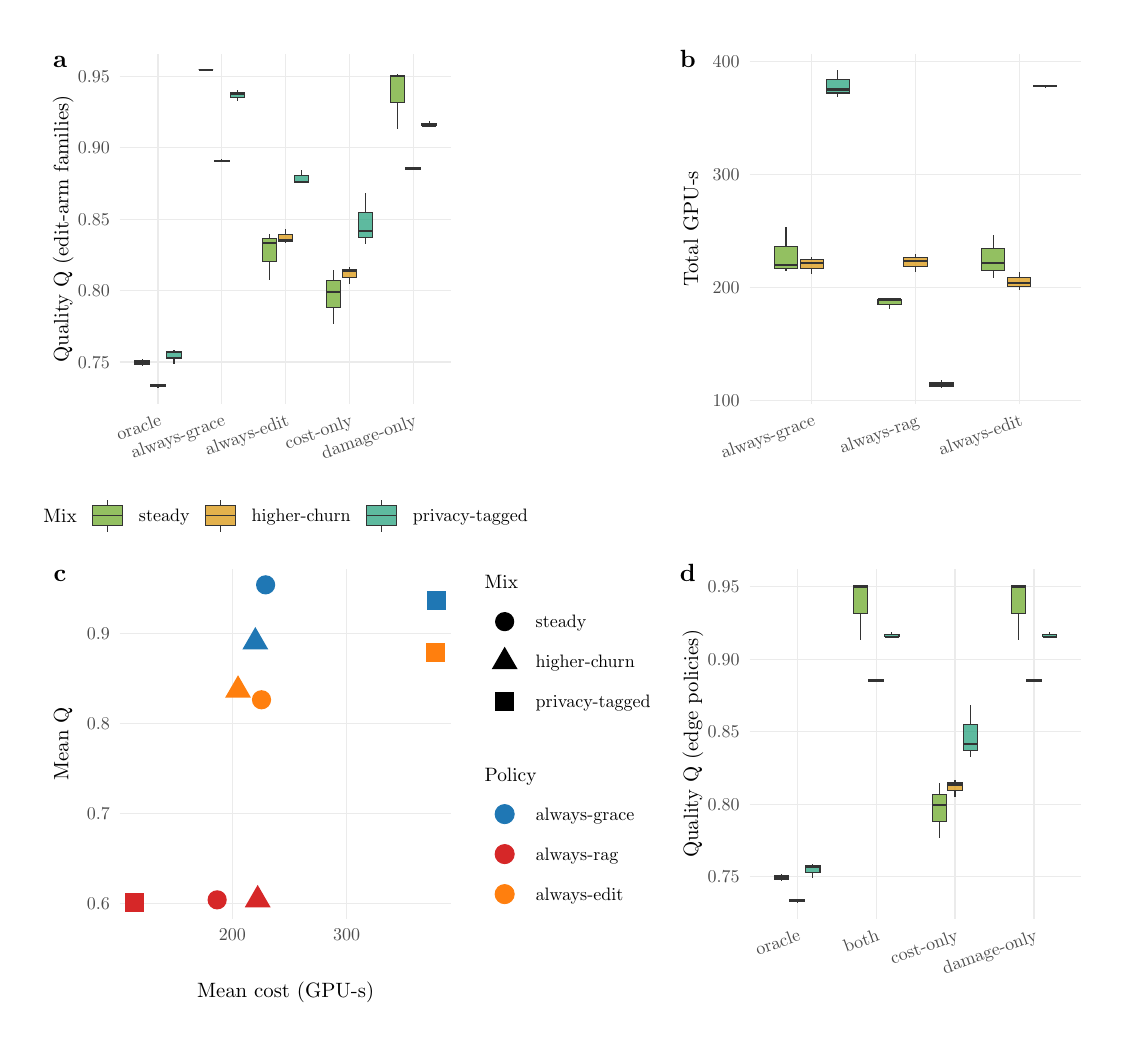
\begin{tikzpicture}[x=1pt,y=1pt]
\definecolor{fillColor}{RGB}{255,255,255}
\path[use as bounding box,fill=fillColor,fill opacity=0.00] (0,0) rectangle (390.26,361.35);
\begin{scope}
\path[clip] (  0.00,  0.00) rectangle (390.26,361.35);
\definecolor{drawColor}{RGB}{255,255,255}
\definecolor{fillColor}{RGB}{255,255,255}

\path[draw=drawColor,line width= 0.6pt,line join=round,line cap=round,fill=fillColor] (  0.00,  0.00) rectangle (390.26,361.35);
\end{scope}
\begin{scope}
\path[clip] (  5.50,169.76) rectangle (233.12,355.85);
\definecolor{fillColor}{RGB}{255,255,255}

\path[fill=fillColor] (  5.50,169.76) rectangle (233.12,355.85);
\end{scope}
\begin{scope}
\path[clip] (233.12,169.76) rectangle (384.76,355.85);
\definecolor{fillColor}{RGB}{255,255,255}

\path[fill=fillColor] (233.12,169.76) rectangle (384.76,355.85);
\end{scope}
\begin{scope}
\path[clip] (  5.50,  5.50) rectangle (233.12,169.76);
\definecolor{fillColor}{RGB}{255,255,255}

\path[fill=fillColor] (  5.50,  5.50) rectangle (233.12,169.76);
\end{scope}
\begin{scope}
\path[clip] (233.12,  5.50) rectangle (384.76,169.76);
\definecolor{fillColor}{RGB}{255,255,255}

\path[fill=fillColor] (233.12,  5.50) rectangle (384.76,169.76);
\end{scope}
\begin{scope}
\path[clip] ( 33.28,225.49) rectangle (153.13,351.85);
\definecolor{drawColor}{gray}{0.92}

\path[draw=drawColor,line width= 0.4pt,line join=round] ( 33.28,240.54) --
	(153.13,240.54);

\path[draw=drawColor,line width= 0.4pt,line join=round] ( 33.28,266.36) --
	(153.13,266.36);

\path[draw=drawColor,line width= 0.4pt,line join=round] ( 33.28,292.19) --
	(153.13,292.19);

\path[draw=drawColor,line width= 0.4pt,line join=round] ( 33.28,318.01) --
	(153.13,318.01);

\path[draw=drawColor,line width= 0.4pt,line join=round] ( 33.28,343.83) --
	(153.13,343.83);

\path[draw=drawColor,line width= 0.4pt,line join=round] ( 47.11,225.49) --
	( 47.11,351.85);

\path[draw=drawColor,line width= 0.4pt,line join=round] ( 70.16,225.49) --
	( 70.16,351.85);

\path[draw=drawColor,line width= 0.4pt,line join=round] ( 93.21,225.49) --
	( 93.21,351.85);

\path[draw=drawColor,line width= 0.4pt,line join=round] (116.25,225.49) --
	(116.25,351.85);

\path[draw=drawColor,line width= 0.4pt,line join=round] (139.30,225.49) --
	(139.30,351.85);
\definecolor{drawColor}{gray}{0.20}

\path[draw=drawColor,line width= 0.4pt,line join=round] ( 41.34,240.95) -- ( 41.34,241.57);

\path[draw=drawColor,line width= 0.4pt,line join=round] ( 41.34,239.71) -- ( 41.34,239.09);
\definecolor{fillColor}{RGB}{102,166,31}

\path[draw=drawColor,line width= 0.4pt,fill=fillColor,fill opacity=0.70] ( 38.75,240.95) --
	( 38.75,239.71) --
	( 43.94,239.71) --
	( 43.94,240.95) --
	( 38.75,240.95) --
	cycle;

\path[draw=drawColor,line width= 0.8pt] ( 38.75,240.33) -- ( 43.94,240.33);

\path[draw=drawColor,line width= 0.4pt,line join=round] ( 47.11,232.27) -- ( 47.11,232.48);

\path[draw=drawColor,line width= 0.4pt,line join=round] ( 47.11,231.65) -- ( 47.11,231.24);
\definecolor{fillColor}{RGB}{216,144,0}

\path[draw=drawColor,line width= 0.4pt,fill=fillColor,fill opacity=0.70] ( 44.51,232.27) --
	( 44.51,231.65) --
	( 49.70,231.65) --
	( 49.70,232.27) --
	( 44.51,232.27) --
	cycle;

\path[draw=drawColor,line width= 0.8pt] ( 44.51,232.06) -- ( 49.70,232.06);

\path[draw=drawColor,line width= 0.4pt,line join=round] ( 52.87,244.47) -- ( 52.87,244.88);

\path[draw=drawColor,line width= 0.4pt,line join=round] ( 52.87,241.99) -- ( 52.87,239.92);
\definecolor{fillColor}{RGB}{27,158,119}

\path[draw=drawColor,line width= 0.4pt,fill=fillColor,fill opacity=0.70] ( 50.28,244.47) --
	( 50.28,241.99) --
	( 55.46,241.99) --
	( 55.46,244.47) --
	( 50.28,244.47) --
	cycle;

\path[draw=drawColor,line width= 0.8pt] ( 50.28,244.05) -- ( 55.46,244.05);

\path[draw=drawColor,line width= 0.4pt,line join=round] ( 64.39,346.11) -- ( 64.39,346.11);

\path[draw=drawColor,line width= 0.4pt,line join=round] ( 64.39,346.11) -- ( 64.39,346.11);
\definecolor{fillColor}{RGB}{102,166,31}

\path[draw=drawColor,line width= 0.4pt,fill=fillColor,fill opacity=0.70] ( 61.80,346.11) --
	( 61.80,346.11) --
	( 66.99,346.11) --
	( 66.99,346.11) --
	( 61.80,346.11) --
	cycle;

\path[draw=drawColor,line width= 0.8pt] ( 61.80,346.11) -- ( 66.99,346.11);

\path[draw=drawColor,line width= 0.4pt,line join=round] ( 70.16,313.46) -- ( 70.16,313.87);

\path[draw=drawColor,line width= 0.4pt,line join=round] ( 70.16,313.05) -- ( 70.16,313.05);
\definecolor{fillColor}{RGB}{216,144,0}

\path[draw=drawColor,line width= 0.4pt,fill=fillColor,fill opacity=0.70] ( 67.56,313.46) --
	( 67.56,313.05) --
	( 72.75,313.05) --
	( 72.75,313.46) --
	( 67.56,313.46) --
	cycle;

\path[draw=drawColor,line width= 0.8pt] ( 67.56,313.05) -- ( 72.75,313.05);

\path[draw=drawColor,line width= 0.4pt,line join=round] ( 75.92,338.05) -- ( 75.92,338.67);

\path[draw=drawColor,line width= 0.4pt,line join=round] ( 75.92,336.19) -- ( 75.92,334.95);
\definecolor{fillColor}{RGB}{27,158,119}

\path[draw=drawColor,line width= 0.4pt,fill=fillColor,fill opacity=0.70] ( 73.32,338.05) --
	( 73.32,336.19) --
	( 78.51,336.19) --
	( 78.51,338.05) --
	( 73.32,338.05) --
	cycle;

\path[draw=drawColor,line width= 0.8pt] ( 73.32,337.43) -- ( 78.51,337.43);

\path[draw=drawColor,line width= 0.4pt,line join=round] ( 87.44,285.08) -- ( 87.44,286.73);

\path[draw=drawColor,line width= 0.4pt,line join=round] ( 87.44,276.77) -- ( 87.44,270.11);
\definecolor{fillColor}{RGB}{102,166,31}

\path[draw=drawColor,line width= 0.4pt,fill=fillColor,fill opacity=0.70] ( 84.85,285.08) --
	( 84.85,276.77) --
	( 90.04,276.77) --
	( 90.04,285.08) --
	( 84.85,285.08) --
	cycle;

\path[draw=drawColor,line width= 0.8pt] ( 84.85,283.42) -- ( 90.04,283.42);

\path[draw=drawColor,line width= 0.4pt,line join=round] ( 93.21,286.57) -- ( 93.21,288.65);

\path[draw=drawColor,line width= 0.4pt,line join=round] ( 93.21,284.06) -- ( 93.21,283.61);
\definecolor{fillColor}{RGB}{216,144,0}

\path[draw=drawColor,line width= 0.4pt,fill=fillColor,fill opacity=0.70] ( 90.61,286.57) --
	( 90.61,284.06) --
	( 95.80,284.06) --
	( 95.80,286.57) --
	( 90.61,286.57) --
	cycle;

\path[draw=drawColor,line width= 0.8pt] ( 90.61,284.50) -- ( 95.80,284.50);

\path[draw=drawColor,line width= 0.4pt,line join=round] ( 98.97,307.90) -- ( 98.97,310.08);

\path[draw=drawColor,line width= 0.4pt,line join=round] ( 98.97,305.64) -- ( 98.97,305.57);
\definecolor{fillColor}{RGB}{27,158,119}

\path[draw=drawColor,line width= 0.4pt,fill=fillColor,fill opacity=0.70] ( 96.37,307.90) --
	( 96.37,305.64) --
	(101.56,305.64) --
	(101.56,307.90) --
	( 96.37,307.90) --
	cycle;

\path[draw=drawColor,line width= 0.8pt] ( 96.37,305.72) -- (101.56,305.72);

\path[draw=drawColor,line width= 0.4pt,line join=round] (110.49,269.91) -- (110.49,273.90);

\path[draw=drawColor,line width= 0.4pt,line join=round] (110.49,260.17) -- (110.49,254.40);
\definecolor{fillColor}{RGB}{102,166,31}

\path[draw=drawColor,line width= 0.4pt,fill=fillColor,fill opacity=0.70] (107.90,269.91) --
	(107.90,260.17) --
	(113.09,260.17) --
	(113.09,269.91) --
	(107.90,269.91) --
	cycle;

\path[draw=drawColor,line width= 0.8pt] (107.90,265.93) -- (113.09,265.93);

\path[draw=drawColor,line width= 0.4pt,line join=round] (116.25,274.09) -- (116.25,274.84);

\path[draw=drawColor,line width= 0.4pt,line join=round] (116.25,271.07) -- (116.25,268.80);
\definecolor{fillColor}{RGB}{216,144,0}

\path[draw=drawColor,line width= 0.4pt,fill=fillColor,fill opacity=0.70] (113.66,274.09) --
	(113.66,271.07) --
	(118.85,271.07) --
	(118.85,274.09) --
	(113.66,274.09) --
	cycle;

\path[draw=drawColor,line width= 0.8pt] (113.66,273.34) -- (118.85,273.34);

\path[draw=drawColor,line width= 0.4pt,line join=round] (122.02,294.72) -- (122.02,301.65);

\path[draw=drawColor,line width= 0.4pt,line join=round] (122.02,285.52) -- (122.02,283.25);
\definecolor{fillColor}{RGB}{27,158,119}

\path[draw=drawColor,line width= 0.4pt,fill=fillColor,fill opacity=0.70] (119.42,294.72) --
	(119.42,285.52) --
	(124.61,285.52) --
	(124.61,294.72) --
	(119.42,294.72) --
	cycle;

\path[draw=drawColor,line width= 0.8pt] (119.42,287.78) -- (124.61,287.78);

\path[draw=drawColor,line width= 0.4pt,line join=round] (133.54,344.22) -- (133.54,344.51);

\path[draw=drawColor,line width= 0.4pt,line join=round] (133.54,334.41) -- (133.54,324.91);
\definecolor{fillColor}{RGB}{102,166,31}

\path[draw=drawColor,line width= 0.4pt,fill=fillColor,fill opacity=0.70] (130.95,344.22) --
	(130.95,334.41) --
	(136.14,334.41) --
	(136.14,344.22) --
	(130.95,344.22) --
	cycle;

\path[draw=drawColor,line width= 0.8pt] (130.95,343.92) -- (136.14,343.92);

\path[draw=drawColor,line width= 0.4pt,line join=round] (139.30,310.64) -- (139.30,310.99);

\path[draw=drawColor,line width= 0.4pt,line join=round] (139.30,310.12) -- (139.30,309.97);
\definecolor{fillColor}{RGB}{216,144,0}

\path[draw=drawColor,line width= 0.4pt,fill=fillColor,fill opacity=0.70] (136.71,310.64) --
	(136.71,310.12) --
	(141.90,310.12) --
	(141.90,310.64) --
	(136.71,310.64) --
	cycle;

\path[draw=drawColor,line width= 0.8pt] (136.71,310.28) -- (141.90,310.28);

\path[draw=drawColor,line width= 0.4pt,line join=round] (145.07,326.78) -- (145.07,327.59);

\path[draw=drawColor,line width= 0.4pt,line join=round] (145.07,325.96) -- (145.07,325.93);
\definecolor{fillColor}{RGB}{27,158,119}

\path[draw=drawColor,line width= 0.4pt,fill=fillColor,fill opacity=0.70] (142.47,326.78) --
	(142.47,325.96) --
	(147.66,325.96) --
	(147.66,326.78) --
	(142.47,326.78) --
	cycle;

\path[draw=drawColor,line width= 0.8pt] (142.47,325.98) -- (147.66,325.98);
\end{scope}
\begin{scope}
\path[clip] (  0.00,  0.00) rectangle (390.26,361.35);
\definecolor{drawColor}{gray}{0.30}

\node[text=drawColor,anchor=base east,inner sep=0pt, outer sep=0pt, scale=  0.65] at ( 29.68,238.30) {0.75};

\node[text=drawColor,anchor=base east,inner sep=0pt, outer sep=0pt, scale=  0.65] at ( 29.68,264.13) {0.80};

\node[text=drawColor,anchor=base east,inner sep=0pt, outer sep=0pt, scale=  0.65] at ( 29.68,289.95) {0.85};

\node[text=drawColor,anchor=base east,inner sep=0pt, outer sep=0pt, scale=  0.65] at ( 29.68,315.77) {0.90};

\node[text=drawColor,anchor=base east,inner sep=0pt, outer sep=0pt, scale=  0.65] at ( 29.68,341.60) {0.95};
\end{scope}
\begin{scope}
\path[clip] (  0.00,  0.00) rectangle (390.26,361.35);
\definecolor{drawColor}{gray}{0.30}

\node[text=drawColor,rotate= 20.00,anchor=base east,inner sep=0pt, outer sep=0pt, scale=  0.65] at ( 48.64,217.69) {oracle};

\node[text=drawColor,rotate= 20.00,anchor=base east,inner sep=0pt, outer sep=0pt, scale=  0.65] at ( 71.69,217.69) {always-grace};

\node[text=drawColor,rotate= 20.00,anchor=base east,inner sep=0pt, outer sep=0pt, scale=  0.65] at ( 94.74,217.69) {always-edit};

\node[text=drawColor,rotate= 20.00,anchor=base east,inner sep=0pt, outer sep=0pt, scale=  0.65] at (117.79,217.69) {cost-only};

\node[text=drawColor,rotate= 20.00,anchor=base east,inner sep=0pt, outer sep=0pt, scale=  0.65] at (140.84,217.69) {damage-only};
\end{scope}
\begin{scope}
\path[clip] (  0.00,  0.00) rectangle (390.26,361.35);
\definecolor{drawColor}{RGB}{0,0,0}

\node[text=drawColor,rotate= 90.00,anchor=base,inner sep=0pt, outer sep=0pt, scale=  0.75] at ( 14.67,288.67) {Quality Q (edit-arm families)};
\end{scope}
\begin{scope}
\path[clip] (  0.00,  0.00) rectangle (390.26,361.35);
\definecolor{drawColor}{RGB}{0,0,0}

\node[text=drawColor,anchor=base west,inner sep=0pt, outer sep=0pt, scale=  0.70] at (  5.71,182.58) {Mix};
\end{scope}
\begin{scope}
\path[clip] (  0.00,  0.00) rectangle (390.26,361.35);
\definecolor{drawColor}{gray}{0.20}

\path[draw=drawColor,line width= 0.4pt] ( 28.99,179.21) --
	( 28.99,181.37);

\path[draw=drawColor,line width= 0.4pt] ( 28.99,188.60) --
	( 28.99,190.77);
\definecolor{fillColor}{RGB}{102,166,31}

\path[draw=drawColor,line width= 0.4pt,fill=fillColor,fill opacity=0.70] ( 23.57,181.37) rectangle ( 34.41,188.60);

\path[draw=drawColor,line width= 0.4pt] ( 23.57,184.99) --
	( 34.41,184.99);

\path[draw=drawColor,line width= 0.4pt] ( 28.99,179.21) --
	( 28.99,179.21);

\path[draw=drawColor,line width= 0.4pt] ( 28.99,190.77) --
	( 28.99,190.77);
\end{scope}
\begin{scope}
\path[clip] (  0.00,  0.00) rectangle (390.26,361.35);
\definecolor{drawColor}{gray}{0.20}

\path[draw=drawColor,line width= 0.4pt] ( 69.71,179.21) --
	( 69.71,181.37);

\path[draw=drawColor,line width= 0.4pt] ( 69.71,188.60) --
	( 69.71,190.77);
\definecolor{fillColor}{RGB}{216,144,0}

\path[draw=drawColor,line width= 0.4pt,fill=fillColor,fill opacity=0.70] ( 64.29,181.37) rectangle ( 75.13,188.60);

\path[draw=drawColor,line width= 0.4pt] ( 64.29,184.99) --
	( 75.13,184.99);

\path[draw=drawColor,line width= 0.4pt] ( 69.71,179.21) --
	( 69.71,179.21);

\path[draw=drawColor,line width= 0.4pt] ( 69.71,190.77) --
	( 69.71,190.77);
\end{scope}
\begin{scope}
\path[clip] (  0.00,  0.00) rectangle (390.26,361.35);
\definecolor{drawColor}{gray}{0.20}

\path[draw=drawColor,line width= 0.4pt] (127.94,179.21) --
	(127.94,181.37);

\path[draw=drawColor,line width= 0.4pt] (127.94,188.60) --
	(127.94,190.77);
\definecolor{fillColor}{RGB}{27,158,119}

\path[draw=drawColor,line width= 0.4pt,fill=fillColor,fill opacity=0.70] (122.52,181.37) rectangle (133.36,188.60);

\path[draw=drawColor,line width= 0.4pt] (122.52,184.99) --
	(133.36,184.99);

\path[draw=drawColor,line width= 0.4pt] (127.94,179.21) --
	(127.94,179.21);

\path[draw=drawColor,line width= 0.4pt] (127.94,190.77) --
	(127.94,190.77);
\end{scope}
\begin{scope}
\path[clip] (  0.00,  0.00) rectangle (390.26,361.35);
\definecolor{drawColor}{RGB}{0,0,0}

\node[text=drawColor,anchor=base west,inner sep=0pt, outer sep=0pt, scale=  0.65] at ( 40.21,182.75) {steady};
\end{scope}
\begin{scope}
\path[clip] (  0.00,  0.00) rectangle (390.26,361.35);
\definecolor{drawColor}{RGB}{0,0,0}

\node[text=drawColor,anchor=base west,inner sep=0pt, outer sep=0pt, scale=  0.65] at ( 80.94,182.75) {higher-churn};
\end{scope}
\begin{scope}
\path[clip] (  0.00,  0.00) rectangle (390.26,361.35);
\definecolor{drawColor}{RGB}{0,0,0}

\node[text=drawColor,anchor=base west,inner sep=0pt, outer sep=0pt, scale=  0.65] at (139.17,182.75) {privacy-tagged};
\end{scope}
\begin{scope}
\path[clip] (  0.00,  0.00) rectangle (390.26,361.35);
\definecolor{drawColor}{RGB}{0,0,0}

\node[text=drawColor,anchor=base,inner sep=0pt, outer sep=0pt, scale=  0.90] at ( 11.70,346.96) {\bfseries a};
\end{scope}
\begin{scope}
\path[clip] (260.90,225.49) rectangle (380.76,351.85);
\definecolor{drawColor}{gray}{0.92}

\path[draw=drawColor,line width= 0.4pt,line join=round] (260.90,226.66) --
	(380.76,226.66);

\path[draw=drawColor,line width= 0.4pt,line join=round] (260.90,267.53) --
	(380.76,267.53);

\path[draw=drawColor,line width= 0.4pt,line join=round] (260.90,308.40) --
	(380.76,308.40);

\path[draw=drawColor,line width= 0.4pt,line join=round] (260.90,349.27) --
	(380.76,349.27);

\path[draw=drawColor,line width= 0.4pt,line join=round] (283.37,225.49) --
	(283.37,351.85);

\path[draw=drawColor,line width= 0.4pt,line join=round] (320.83,225.49) --
	(320.83,351.85);

\path[draw=drawColor,line width= 0.4pt,line join=round] (358.28,225.49) --
	(358.28,351.85);
\definecolor{drawColor}{gray}{0.20}

\path[draw=drawColor,line width= 0.4pt,line join=round] (274.01,282.35) -- (274.01,289.25);

\path[draw=drawColor,line width= 0.4pt,line join=round] (274.01,274.46) -- (274.01,273.46);
\definecolor{fillColor}{RGB}{102,166,31}

\path[draw=drawColor,line width= 0.4pt,fill=fillColor,fill opacity=0.70] (269.80,282.35) --
	(269.80,274.46) --
	(278.22,274.46) --
	(278.22,282.35) --
	(269.80,282.35) --
	cycle;

\path[draw=drawColor,line width= 0.8pt] (269.80,275.45) -- (278.22,275.45);

\path[draw=drawColor,line width= 0.4pt,line join=round] (283.37,277.42) -- (283.37,278.46);

\path[draw=drawColor,line width= 0.4pt,line join=round] (283.37,274.33) -- (283.37,272.27);
\definecolor{fillColor}{RGB}{216,144,0}

\path[draw=drawColor,line width= 0.4pt,fill=fillColor,fill opacity=0.70] (279.16,277.42) --
	(279.16,274.33) --
	(287.59,274.33) --
	(287.59,277.42) --
	(279.16,277.42) --
	cycle;

\path[draw=drawColor,line width= 0.8pt] (279.16,276.39) -- (287.59,276.39);

\path[draw=drawColor,line width= 0.4pt,line join=round] (292.74,342.55) -- (292.74,346.11);

\path[draw=drawColor,line width= 0.4pt,line join=round] (292.74,337.73) -- (292.74,336.47);
\definecolor{fillColor}{RGB}{27,158,119}

\path[draw=drawColor,line width= 0.4pt,fill=fillColor,fill opacity=0.70] (288.52,342.55) --
	(288.52,337.73) --
	(296.95,337.73) --
	(296.95,342.55) --
	(288.52,342.55) --
	cycle;

\path[draw=drawColor,line width= 0.8pt] (288.52,338.99) -- (296.95,338.99);

\path[draw=drawColor,line width= 0.4pt,line join=round] (311.46,263.20) -- (311.46,263.27);

\path[draw=drawColor,line width= 0.4pt,line join=round] (311.46,261.43) -- (311.46,259.72);
\definecolor{fillColor}{RGB}{102,166,31}

\path[draw=drawColor,line width= 0.4pt,fill=fillColor,fill opacity=0.70] (307.25,263.20) --
	(307.25,261.43) --
	(315.68,261.43) --
	(315.68,263.20) --
	(307.25,263.20) --
	cycle;

\path[draw=drawColor,line width= 0.8pt] (307.25,263.14) -- (315.68,263.14);

\path[draw=drawColor,line width= 0.4pt,line join=round] (320.83,278.21) -- (320.83,279.48);

\path[draw=drawColor,line width= 0.4pt,line join=round] (320.83,275.08) -- (320.83,273.22);
\definecolor{fillColor}{RGB}{216,144,0}

\path[draw=drawColor,line width= 0.4pt,fill=fillColor,fill opacity=0.70] (316.62,278.21) --
	(316.62,275.08) --
	(325.04,275.08) --
	(325.04,278.21) --
	(316.62,278.21) --
	cycle;

\path[draw=drawColor,line width= 0.8pt] (316.62,276.94) -- (325.04,276.94);

\path[draw=drawColor,line width= 0.4pt,line join=round] (330.19,233.23) -- (330.19,234.04);

\path[draw=drawColor,line width= 0.4pt,line join=round] (330.19,231.83) -- (330.19,231.24);
\definecolor{fillColor}{RGB}{27,158,119}

\path[draw=drawColor,line width= 0.4pt,fill=fillColor,fill opacity=0.70] (325.98,233.23) --
	(325.98,231.83) --
	(334.41,231.83) --
	(334.41,233.23) --
	(325.98,233.23) --
	cycle;

\path[draw=drawColor,line width= 0.8pt] (325.98,232.43) -- (334.41,232.43);

\path[draw=drawColor,line width= 0.4pt,line join=round] (348.92,281.49) -- (348.92,286.52);

\path[draw=drawColor,line width= 0.4pt,line join=round] (348.92,273.62) -- (348.92,270.79);
\definecolor{fillColor}{RGB}{102,166,31}

\path[draw=drawColor,line width= 0.4pt,fill=fillColor,fill opacity=0.70] (344.71,281.49) --
	(344.71,273.62) --
	(353.13,273.62) --
	(353.13,281.49) --
	(344.71,281.49) --
	cycle;

\path[draw=drawColor,line width= 0.8pt] (344.71,276.45) -- (353.13,276.45);

\path[draw=drawColor,line width= 0.4pt,line join=round] (358.28,270.98) -- (358.28,272.90);

\path[draw=drawColor,line width= 0.4pt,line join=round] (358.28,267.82) -- (358.28,266.57);
\definecolor{fillColor}{RGB}{216,144,0}

\path[draw=drawColor,line width= 0.4pt,fill=fillColor,fill opacity=0.70] (354.07,270.98) --
	(354.07,267.82) --
	(362.50,267.82) --
	(362.50,270.98) --
	(354.07,270.98) --
	cycle;

\path[draw=drawColor,line width= 0.8pt] (354.07,269.07) -- (362.50,269.07);

\path[draw=drawColor,line width= 0.4pt,line join=round] (367.65,340.59) -- (367.65,340.77);

\path[draw=drawColor,line width= 0.4pt,line join=round] (367.65,339.98) -- (367.65,339.55);
\definecolor{fillColor}{RGB}{27,158,119}

\path[draw=drawColor,line width= 0.4pt,fill=fillColor,fill opacity=0.70] (363.43,340.59) --
	(363.43,339.98) --
	(371.86,339.98) --
	(371.86,340.59) --
	(363.43,340.59) --
	cycle;

\path[draw=drawColor,line width= 0.8pt] (363.43,340.41) -- (371.86,340.41);
\end{scope}
\begin{scope}
\path[clip] (  0.00,  0.00) rectangle (390.26,361.35);
\definecolor{drawColor}{gray}{0.30}

\node[text=drawColor,anchor=base east,inner sep=0pt, outer sep=0pt, scale=  0.65] at (257.30,224.42) {100};

\node[text=drawColor,anchor=base east,inner sep=0pt, outer sep=0pt, scale=  0.65] at (257.30,265.29) {200};

\node[text=drawColor,anchor=base east,inner sep=0pt, outer sep=0pt, scale=  0.65] at (257.30,306.16) {300};

\node[text=drawColor,anchor=base east,inner sep=0pt, outer sep=0pt, scale=  0.65] at (257.30,347.03) {400};
\end{scope}
\begin{scope}
\path[clip] (  0.00,  0.00) rectangle (390.26,361.35);
\definecolor{drawColor}{gray}{0.30}

\node[text=drawColor,rotate= 20.00,anchor=base east,inner sep=0pt, outer sep=0pt, scale=  0.65] at (284.90,217.69) {always-grace};

\node[text=drawColor,rotate= 20.00,anchor=base east,inner sep=0pt, outer sep=0pt, scale=  0.65] at (322.36,217.69) {always-rag};

\node[text=drawColor,rotate= 20.00,anchor=base east,inner sep=0pt, outer sep=0pt, scale=  0.65] at (359.82,217.69) {always-edit};
\end{scope}
\begin{scope}
\path[clip] (  0.00,  0.00) rectangle (390.26,361.35);
\definecolor{drawColor}{RGB}{0,0,0}

\node[text=drawColor,rotate= 90.00,anchor=base,inner sep=0pt, outer sep=0pt, scale=  0.75] at (242.29,288.67) {Total GPU-s};
\end{scope}
\begin{scope}
\path[clip] (  0.00,  0.00) rectangle (390.26,361.35);
\definecolor{drawColor}{RGB}{0,0,0}

\node[text=drawColor,anchor=base,inner sep=0pt, outer sep=0pt, scale=  0.90] at (238.56,346.96) {\bfseries b};
\end{scope}
\begin{scope}
\path[clip] ( 33.28, 39.40) rectangle (153.13,165.76);
\definecolor{drawColor}{gray}{0.92}

\path[draw=drawColor,line width= 0.4pt,line join=round] ( 33.28, 44.89) --
	(153.13, 44.89);

\path[draw=drawColor,line width= 0.4pt,line join=round] ( 33.28, 77.37) --
	(153.13, 77.37);

\path[draw=drawColor,line width= 0.4pt,line join=round] ( 33.28,109.86) --
	(153.13,109.86);

\path[draw=drawColor,line width= 0.4pt,line join=round] ( 33.28,142.34) --
	(153.13,142.34);

\path[draw=drawColor,line width= 0.4pt,line join=round] ( 74.01, 39.40) --
	( 74.01,165.76);

\path[draw=drawColor,line width= 0.4pt,line join=round] (115.26, 39.40) --
	(115.26,165.76);
\definecolor{fillColor}{RGB}{31,119,180}

\path[fill=fillColor] ( 85.98,160.02) circle (  3.47);
\definecolor{fillColor}{RGB}{214,39,40}

\path[fill=fillColor] ( 68.47, 46.19) circle (  3.47);
\definecolor{fillColor}{RGB}{255,127,14}

\path[fill=fillColor] ( 84.50,118.49) circle (  3.47);
\definecolor{fillColor}{RGB}{31,119,180}

\path[fill=fillColor] ( 82.26,144.79) --
	( 86.94,136.69) --
	( 77.59,136.69) --
	cycle;
\definecolor{fillColor}{RGB}{214,39,40}

\path[fill=fillColor] ( 83.11, 51.59) --
	( 87.79, 43.49) --
	( 78.44, 43.49) --
	cycle;
\definecolor{fillColor}{RGB}{255,127,14}

\path[fill=fillColor] ( 76.01,127.35) --
	( 80.69,119.25) --
	( 71.34,119.25) --
	cycle;
\definecolor{fillColor}{RGB}{31,119,180}

\path[fill=fillColor] (144.21,150.83) --
	(151.16,150.83) --
	(151.16,157.77) --
	(144.21,157.77) --
	cycle;
\definecolor{fillColor}{RGB}{214,39,40}

\path[fill=fillColor] ( 35.25, 41.68) --
	( 42.20, 41.68) --
	( 42.20, 48.62) --
	( 35.25, 48.62) --
	cycle;
\definecolor{fillColor}{RGB}{255,127,14}

\path[fill=fillColor] (143.93,132.02) --
	(150.87,132.02) --
	(150.87,138.97) --
	(143.93,138.97) --
	cycle;
\end{scope}
\begin{scope}
\path[clip] (  0.00,  0.00) rectangle (390.26,361.35);
\definecolor{drawColor}{gray}{0.30}

\node[text=drawColor,anchor=base east,inner sep=0pt, outer sep=0pt, scale=  0.65] at ( 29.68, 42.65) {0.6};

\node[text=drawColor,anchor=base east,inner sep=0pt, outer sep=0pt, scale=  0.65] at ( 29.68, 75.13) {0.7};

\node[text=drawColor,anchor=base east,inner sep=0pt, outer sep=0pt, scale=  0.65] at ( 29.68,107.62) {0.8};

\node[text=drawColor,anchor=base east,inner sep=0pt, outer sep=0pt, scale=  0.65] at ( 29.68,140.11) {0.9};
\end{scope}
\begin{scope}
\path[clip] (  0.00,  0.00) rectangle (390.26,361.35);
\definecolor{drawColor}{gray}{0.30}

\node[text=drawColor,anchor=base,inner sep=0pt, outer sep=0pt, scale=  0.65] at ( 74.01, 31.33) {200};

\node[text=drawColor,anchor=base,inner sep=0pt, outer sep=0pt, scale=  0.65] at (115.26, 31.33) {300};
\end{scope}
\begin{scope}
\path[clip] (  0.00,  0.00) rectangle (390.26,361.35);
\definecolor{drawColor}{RGB}{0,0,0}

\node[text=drawColor,anchor=base,inner sep=0pt, outer sep=0pt, scale=  0.75] at ( 93.21, 10.96) {Mean cost (GPU-s)};
\end{scope}
\begin{scope}
\path[clip] (  0.00,  0.00) rectangle (390.26,361.35);
\definecolor{drawColor}{RGB}{0,0,0}

\node[text=drawColor,rotate= 90.00,anchor=base,inner sep=0pt, outer sep=0pt, scale=  0.75] at ( 14.67,102.58) {Mean Q};
\end{scope}
\begin{scope}
\path[clip] (  0.00,  0.00) rectangle (390.26,361.35);
\definecolor{drawColor}{RGB}{0,0,0}

\node[text=drawColor,anchor=base west,inner sep=0pt, outer sep=0pt, scale=  0.70] at (165.13,158.62) {Mix};
\end{scope}
\begin{scope}
\path[clip] (  0.00,  0.00) rectangle (390.26,361.35);
\definecolor{fillColor}{RGB}{0,0,0}

\path[fill=fillColor] (172.36,146.72) circle (  3.47);
\end{scope}
\begin{scope}
\path[clip] (  0.00,  0.00) rectangle (390.26,361.35);
\definecolor{fillColor}{RGB}{0,0,0}

\path[fill=fillColor] (172.36,137.66) --
	(177.04,129.56) --
	(167.69,129.56) --
	cycle;
\end{scope}
\begin{scope}
\path[clip] (  0.00,  0.00) rectangle (390.26,361.35);
\definecolor{fillColor}{RGB}{0,0,0}

\path[fill=fillColor] (168.89,114.34) --
	(175.83,114.34) --
	(175.83,121.28) --
	(168.89,121.28) --
	cycle;
\end{scope}
\begin{scope}
\path[clip] (  0.00,  0.00) rectangle (390.26,361.35);
\definecolor{drawColor}{RGB}{0,0,0}

\node[text=drawColor,anchor=base west,inner sep=0pt, outer sep=0pt, scale=  0.65] at (183.59,144.48) {steady};
\end{scope}
\begin{scope}
\path[clip] (  0.00,  0.00) rectangle (390.26,361.35);
\definecolor{drawColor}{RGB}{0,0,0}

\node[text=drawColor,anchor=base west,inner sep=0pt, outer sep=0pt, scale=  0.65] at (183.59,130.02) {higher-churn};
\end{scope}
\begin{scope}
\path[clip] (  0.00,  0.00) rectangle (390.26,361.35);
\definecolor{drawColor}{RGB}{0,0,0}

\node[text=drawColor,anchor=base west,inner sep=0pt, outer sep=0pt, scale=  0.65] at (183.59,115.57) {privacy-tagged};
\end{scope}
\begin{scope}
\path[clip] (  0.00,  0.00) rectangle (390.26,361.35);
\definecolor{drawColor}{RGB}{0,0,0}

\node[text=drawColor,anchor=base west,inner sep=0pt, outer sep=0pt, scale=  0.70] at (165.13, 89.08) {Policy};
\end{scope}
\begin{scope}
\path[clip] (  0.00,  0.00) rectangle (390.26,361.35);
\definecolor{drawColor}{RGB}{31,119,180}
\definecolor{fillColor}{RGB}{31,119,180}

\path[draw=drawColor,line width= 0.3pt,line join=round,line cap=round,fill=fillColor] (172.36, 77.17) circle (  3.47);
\end{scope}
\begin{scope}
\path[clip] (  0.00,  0.00) rectangle (390.26,361.35);
\definecolor{drawColor}{RGB}{214,39,40}
\definecolor{fillColor}{RGB}{214,39,40}

\path[draw=drawColor,line width= 0.3pt,line join=round,line cap=round,fill=fillColor] (172.36, 62.72) circle (  3.47);
\end{scope}
\begin{scope}
\path[clip] (  0.00,  0.00) rectangle (390.26,361.35);
\definecolor{drawColor}{RGB}{255,127,14}
\definecolor{fillColor}{RGB}{255,127,14}

\path[draw=drawColor,line width= 0.3pt,line join=round,line cap=round,fill=fillColor] (172.36, 48.26) circle (  3.47);
\end{scope}
\begin{scope}
\path[clip] (  0.00,  0.00) rectangle (390.26,361.35);
\definecolor{drawColor}{RGB}{0,0,0}

\node[text=drawColor,anchor=base west,inner sep=0pt, outer sep=0pt, scale=  0.65] at (183.59, 74.93) {always-grace};
\end{scope}
\begin{scope}
\path[clip] (  0.00,  0.00) rectangle (390.26,361.35);
\definecolor{drawColor}{RGB}{0,0,0}

\node[text=drawColor,anchor=base west,inner sep=0pt, outer sep=0pt, scale=  0.65] at (183.59, 60.48) {always-rag};
\end{scope}
\begin{scope}
\path[clip] (  0.00,  0.00) rectangle (390.26,361.35);
\definecolor{drawColor}{RGB}{0,0,0}

\node[text=drawColor,anchor=base west,inner sep=0pt, outer sep=0pt, scale=  0.65] at (183.59, 46.03) {always-edit};
\end{scope}
\begin{scope}
\path[clip] (  0.00,  0.00) rectangle (390.26,361.35);
\definecolor{drawColor}{RGB}{0,0,0}

\node[text=drawColor,anchor=base,inner sep=0pt, outer sep=0pt, scale=  0.90] at ( 11.70,161.09) {\bfseries c};
\end{scope}
\begin{scope}
\path[clip] (260.90, 39.40) rectangle (380.76,165.76);
\definecolor{drawColor}{gray}{0.92}

\path[draw=drawColor,line width= 0.4pt,line join=round] (260.90, 54.58) --
	(380.76, 54.58);

\path[draw=drawColor,line width= 0.4pt,line join=round] (260.90, 80.77) --
	(380.76, 80.77);

\path[draw=drawColor,line width= 0.4pt,line join=round] (260.90,106.96) --
	(380.76,106.96);

\path[draw=drawColor,line width= 0.4pt,line join=round] (260.90,133.14) --
	(380.76,133.14);

\path[draw=drawColor,line width= 0.4pt,line join=round] (260.90,159.33) --
	(380.76,159.33);

\path[draw=drawColor,line width= 0.4pt,line join=round] (278.02, 39.40) --
	(278.02,165.76);

\path[draw=drawColor,line width= 0.4pt,line join=round] (306.56, 39.40) --
	(306.56,165.76);

\path[draw=drawColor,line width= 0.4pt,line join=round] (335.10, 39.40) --
	(335.10,165.76);

\path[draw=drawColor,line width= 0.4pt,line join=round] (363.64, 39.40) --
	(363.64,165.76);
\definecolor{drawColor}{gray}{0.20}

\path[draw=drawColor,line width= 0.4pt,line join=round] (272.31, 55.00) -- (272.31, 55.63);

\path[draw=drawColor,line width= 0.4pt,line join=round] (272.31, 53.74) -- (272.31, 53.11);
\definecolor{fillColor}{RGB}{102,166,31}

\path[draw=drawColor,line width= 0.4pt,fill=fillColor,fill opacity=0.70] (269.75, 55.00) --
	(269.75, 53.74) --
	(274.88, 53.74) --
	(274.88, 55.00) --
	(269.75, 55.00) --
	cycle;

\path[draw=drawColor,line width= 0.8pt] (269.75, 54.37) -- (274.88, 54.37);

\path[draw=drawColor,line width= 0.4pt,line join=round] (278.02, 46.20) -- (278.02, 46.41);

\path[draw=drawColor,line width= 0.4pt,line join=round] (278.02, 45.57) -- (278.02, 45.15);
\definecolor{fillColor}{RGB}{216,144,0}

\path[draw=drawColor,line width= 0.4pt,fill=fillColor,fill opacity=0.70] (275.45, 46.20) --
	(275.45, 45.57) --
	(280.59, 45.57) --
	(280.59, 46.20) --
	(275.45, 46.20) --
	cycle;

\path[draw=drawColor,line width= 0.8pt] (275.45, 45.98) -- (280.59, 45.98);

\path[draw=drawColor,line width= 0.4pt,line join=round] (283.73, 58.56) -- (283.73, 58.98);

\path[draw=drawColor,line width= 0.4pt,line join=round] (283.73, 56.05) -- (283.73, 53.95);
\definecolor{fillColor}{RGB}{27,158,119}

\path[draw=drawColor,line width= 0.4pt,fill=fillColor,fill opacity=0.70] (281.16, 58.56) --
	(281.16, 56.05) --
	(286.30, 56.05) --
	(286.30, 58.56) --
	(281.16, 58.56) --
	cycle;

\path[draw=drawColor,line width= 0.8pt] (281.16, 58.14) -- (286.30, 58.14);

\path[draw=drawColor,line width= 0.4pt,line join=round] (300.85,159.72) -- (300.85,160.02);

\path[draw=drawColor,line width= 0.4pt,line join=round] (300.85,149.78) -- (300.85,140.14);
\definecolor{fillColor}{RGB}{102,166,31}

\path[draw=drawColor,line width= 0.4pt,fill=fillColor,fill opacity=0.70] (298.28,159.72) --
	(298.28,149.78) --
	(303.42,149.78) --
	(303.42,159.72) --
	(298.28,159.72) --
	cycle;

\path[draw=drawColor,line width= 0.8pt] (298.28,159.42) -- (303.42,159.42);

\path[draw=drawColor,line width= 0.4pt,line join=round] (306.56,125.66) -- (306.56,126.03);

\path[draw=drawColor,line width= 0.4pt,line join=round] (306.56,125.14) -- (306.56,124.99);
\definecolor{fillColor}{RGB}{216,144,0}

\path[draw=drawColor,line width= 0.4pt,fill=fillColor,fill opacity=0.70] (303.99,125.66) --
	(303.99,125.14) --
	(309.13,125.14) --
	(309.13,125.66) --
	(303.99,125.66) --
	cycle;

\path[draw=drawColor,line width= 0.8pt] (303.99,125.30) -- (309.13,125.30);

\path[draw=drawColor,line width= 0.4pt,line join=round] (312.27,142.04) -- (312.27,142.86);

\path[draw=drawColor,line width= 0.4pt,line join=round] (312.27,141.20) -- (312.27,141.17);
\definecolor{fillColor}{RGB}{27,158,119}

\path[draw=drawColor,line width= 0.4pt,fill=fillColor,fill opacity=0.70] (309.70,142.04) --
	(309.70,141.20) --
	(314.84,141.20) --
	(314.84,142.04) --
	(309.70,142.04) --
	cycle;

\path[draw=drawColor,line width= 0.8pt] (309.70,141.22) -- (314.84,141.22);

\path[draw=drawColor,line width= 0.4pt,line join=round] (329.39, 84.37) -- (329.39, 88.41);

\path[draw=drawColor,line width= 0.4pt,line join=round] (329.39, 74.48) -- (329.39, 68.64);
\definecolor{fillColor}{RGB}{102,166,31}

\path[draw=drawColor,line width= 0.4pt,fill=fillColor,fill opacity=0.70] (326.82, 84.37) --
	(326.82, 74.48) --
	(331.96, 74.48) --
	(331.96, 84.37) --
	(326.82, 84.37) --
	cycle;

\path[draw=drawColor,line width= 0.8pt] (326.82, 80.33) -- (331.96, 80.33);

\path[draw=drawColor,line width= 0.4pt,line join=round] (335.10, 88.60) -- (335.10, 89.36);

\path[draw=drawColor,line width= 0.4pt,line join=round] (335.10, 85.54) -- (335.10, 83.24);
\definecolor{fillColor}{RGB}{216,144,0}

\path[draw=drawColor,line width= 0.4pt,fill=fillColor,fill opacity=0.70] (332.53, 88.60) --
	(332.53, 85.54) --
	(337.67, 85.54) --
	(337.67, 88.60) --
	(332.53, 88.60) --
	cycle;

\path[draw=drawColor,line width= 0.8pt] (332.53, 87.84) -- (337.67, 87.84);

\path[draw=drawColor,line width= 0.4pt,line join=round] (340.81,109.52) -- (340.81,116.56);

\path[draw=drawColor,line width= 0.4pt,line join=round] (340.81,100.19) -- (340.81, 97.89);
\definecolor{fillColor}{RGB}{27,158,119}

\path[draw=drawColor,line width= 0.4pt,fill=fillColor,fill opacity=0.70] (338.24,109.52) --
	(338.24,100.19) --
	(343.37,100.19) --
	(343.37,109.52) --
	(338.24,109.52) --
	cycle;

\path[draw=drawColor,line width= 0.8pt] (338.24,102.49) -- (343.37,102.49);

\path[draw=drawColor,line width= 0.4pt,line join=round] (357.93,159.72) -- (357.93,160.02);

\path[draw=drawColor,line width= 0.4pt,line join=round] (357.93,149.78) -- (357.93,140.14);
\definecolor{fillColor}{RGB}{102,166,31}

\path[draw=drawColor,line width= 0.4pt,fill=fillColor,fill opacity=0.70] (355.36,159.72) --
	(355.36,149.78) --
	(360.50,149.78) --
	(360.50,159.72) --
	(355.36,159.72) --
	cycle;

\path[draw=drawColor,line width= 0.8pt] (355.36,159.42) -- (360.50,159.42);

\path[draw=drawColor,line width= 0.4pt,line join=round] (363.64,125.66) -- (363.64,126.03);

\path[draw=drawColor,line width= 0.4pt,line join=round] (363.64,125.14) -- (363.64,124.99);
\definecolor{fillColor}{RGB}{216,144,0}

\path[draw=drawColor,line width= 0.4pt,fill=fillColor,fill opacity=0.70] (361.07,125.66) --
	(361.07,125.14) --
	(366.20,125.14) --
	(366.20,125.66) --
	(361.07,125.66) --
	cycle;

\path[draw=drawColor,line width= 0.8pt] (361.07,125.30) -- (366.20,125.30);

\path[draw=drawColor,line width= 0.4pt,line join=round] (369.34,142.04) -- (369.34,142.86);

\path[draw=drawColor,line width= 0.4pt,line join=round] (369.34,141.20) -- (369.34,141.17);
\definecolor{fillColor}{RGB}{27,158,119}

\path[draw=drawColor,line width= 0.4pt,fill=fillColor,fill opacity=0.70] (366.77,142.04) --
	(366.77,141.20) --
	(371.91,141.20) --
	(371.91,142.04) --
	(366.77,142.04) --
	cycle;

\path[draw=drawColor,line width= 0.8pt] (366.77,141.22) -- (371.91,141.22);
\end{scope}
\begin{scope}
\path[clip] (  0.00,  0.00) rectangle (390.26,361.35);
\definecolor{drawColor}{gray}{0.30}

\node[text=drawColor,anchor=base east,inner sep=0pt, outer sep=0pt, scale=  0.65] at (257.30, 52.34) {0.75};

\node[text=drawColor,anchor=base east,inner sep=0pt, outer sep=0pt, scale=  0.65] at (257.30, 78.53) {0.80};

\node[text=drawColor,anchor=base east,inner sep=0pt, outer sep=0pt, scale=  0.65] at (257.30,104.72) {0.85};

\node[text=drawColor,anchor=base east,inner sep=0pt, outer sep=0pt, scale=  0.65] at (257.30,130.90) {0.90};

\node[text=drawColor,anchor=base east,inner sep=0pt, outer sep=0pt, scale=  0.65] at (257.30,157.09) {0.95};
\end{scope}
\begin{scope}
\path[clip] (  0.00,  0.00) rectangle (390.26,361.35);
\definecolor{drawColor}{gray}{0.30}

\node[text=drawColor,rotate= 20.00,anchor=base east,inner sep=0pt, outer sep=0pt, scale=  0.65] at (279.55, 31.60) {oracle};

\node[text=drawColor,rotate= 20.00,anchor=base east,inner sep=0pt, outer sep=0pt, scale=  0.65] at (308.09, 31.60) {both};

\node[text=drawColor,rotate= 20.00,anchor=base east,inner sep=0pt, outer sep=0pt, scale=  0.65] at (336.63, 31.60) {cost-only};

\node[text=drawColor,rotate= 20.00,anchor=base east,inner sep=0pt, outer sep=0pt, scale=  0.65] at (365.17, 31.60) {damage-only};
\end{scope}
\begin{scope}
\path[clip] (  0.00,  0.00) rectangle (390.26,361.35);
\definecolor{drawColor}{RGB}{0,0,0}

\node[text=drawColor,rotate= 90.00,anchor=base,inner sep=0pt, outer sep=0pt, scale=  0.75] at (242.29,102.58) {Quality Q (edge policies)};
\end{scope}
\begin{scope}
\path[clip] (  0.00,  0.00) rectangle (390.26,361.35);
\definecolor{drawColor}{RGB}{0,0,0}

\node[text=drawColor,anchor=base,inner sep=0pt, outer sep=0pt, scale=  0.90] at (238.56,161.09) {\bfseries d};
\end{scope}
\end{tikzpicture}

\caption{Quality and cost distributions across stream configurations. Panels (a)/(b)
show per-seed quality $Q$ and total GPU-s for the edit-arm policy families; panels
(c)/(d) contrast the always-grace / always-rag / always-edit operating points and the
edge policies. The codebook (always-grace) policy sits at the top of the quality
distribution at competitive cost.}
\label{fig:failure-modes-app}
\end{figure}

\begin{figure}[!ht]
\centering
% SOURCE: edit-harness/results/frame_a/cells/cell_*_real_MIX_{A,B,C}_*.json
% !TEX encoding = UTF-8 Unicode
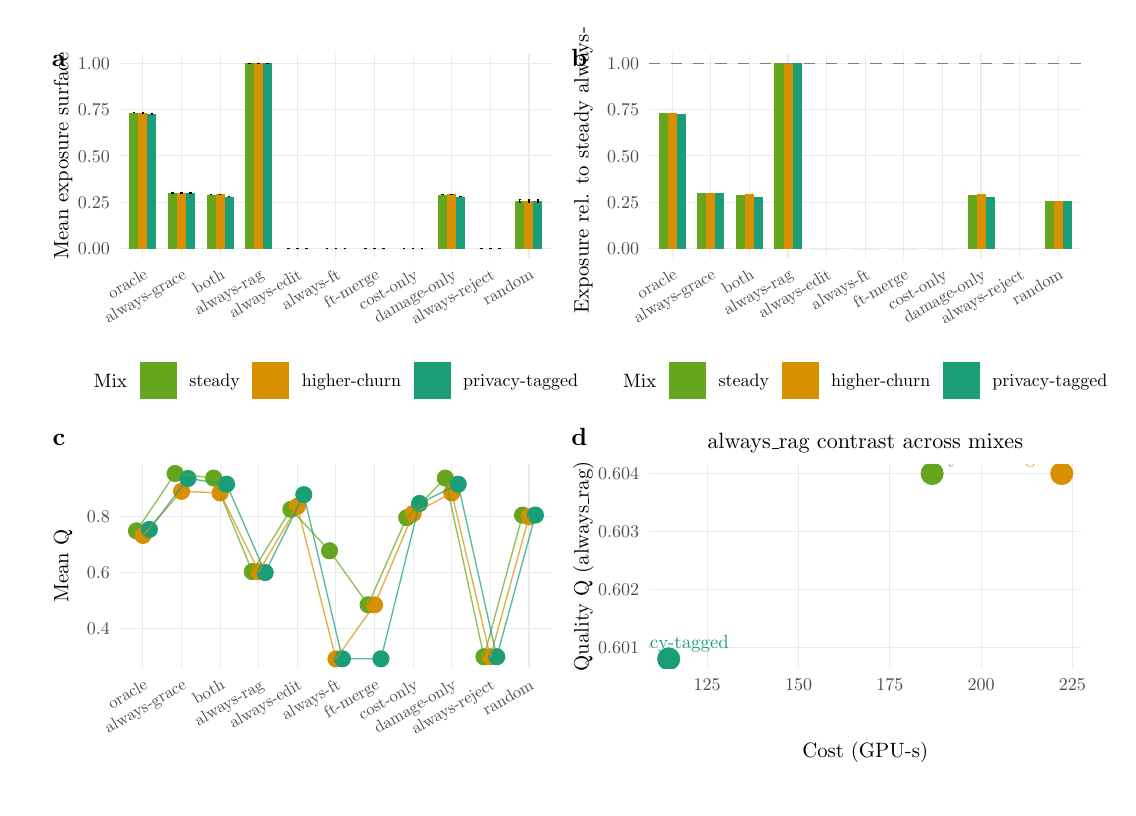
\begin{tikzpicture}[x=1pt,y=1pt]
\definecolor{fillColor}{RGB}{255,255,255}
\path[use as bounding box,fill=fillColor,fill opacity=0.00] (0,0) rectangle (390.26,274.63);
\begin{scope}
\path[clip] (  0.00,  0.00) rectangle (390.26,274.63);
\definecolor{drawColor}{RGB}{255,255,255}
\definecolor{fillColor}{RGB}{255,255,255}

\path[draw=drawColor,line width= 0.6pt,line join=round,line cap=round,fill=fillColor] (  0.00,  0.00) rectangle (390.26,274.63);
\end{scope}
\begin{scope}
\path[clip] (  5.50,131.93) rectangle (193.50,269.13);
\definecolor{fillColor}{RGB}{255,255,255}

\path[fill=fillColor] (  5.50,131.93) rectangle (193.50,269.13);
\end{scope}
\begin{scope}
\path[clip] (193.50,131.93) rectangle (384.76,269.13);
\definecolor{fillColor}{RGB}{255,255,255}

\path[fill=fillColor] (193.50,131.93) rectangle (384.76,269.13);
\end{scope}
\begin{scope}
\path[clip] (  5.50,  5.50) rectangle (193.50,131.93);
\definecolor{fillColor}{RGB}{255,255,255}

\path[fill=fillColor] (  5.50,  5.50) rectangle (193.50,131.93);
\end{scope}
\begin{scope}
\path[clip] (193.50,  5.50) rectangle (384.76,131.93);
\definecolor{fillColor}{RGB}{255,255,255}

\path[fill=fillColor] (193.50,  5.50) rectangle (384.76,131.93);
\end{scope}
\begin{scope}
\path[clip] ( 33.28,191.43) rectangle (189.50,265.13);
\definecolor{drawColor}{gray}{0.92}

\path[draw=drawColor,line width= 0.4pt,line join=round] ( 33.28,194.78) --
	(189.50,194.78);

\path[draw=drawColor,line width= 0.4pt,line join=round] ( 33.28,211.53) --
	(189.50,211.53);

\path[draw=drawColor,line width= 0.4pt,line join=round] ( 33.28,228.28) --
	(189.50,228.28);

\path[draw=drawColor,line width= 0.4pt,line join=round] ( 33.28,245.03) --
	(189.50,245.03);

\path[draw=drawColor,line width= 0.4pt,line join=round] ( 33.28,261.78) --
	(189.50,261.78);

\path[draw=drawColor,line width= 0.4pt,line join=round] ( 41.65,191.43) --
	( 41.65,265.13);

\path[draw=drawColor,line width= 0.4pt,line join=round] ( 55.59,191.43) --
	( 55.59,265.13);

\path[draw=drawColor,line width= 0.4pt,line join=round] ( 69.54,191.43) --
	( 69.54,265.13);

\path[draw=drawColor,line width= 0.4pt,line join=round] ( 83.49,191.43) --
	( 83.49,265.13);

\path[draw=drawColor,line width= 0.4pt,line join=round] ( 97.44,191.43) --
	( 97.44,265.13);

\path[draw=drawColor,line width= 0.4pt,line join=round] (111.39,191.43) --
	(111.39,265.13);

\path[draw=drawColor,line width= 0.4pt,line join=round] (125.34,191.43) --
	(125.34,265.13);

\path[draw=drawColor,line width= 0.4pt,line join=round] (139.29,191.43) --
	(139.29,265.13);

\path[draw=drawColor,line width= 0.4pt,line join=round] (153.24,191.43) --
	(153.24,265.13);

\path[draw=drawColor,line width= 0.4pt,line join=round] (167.19,191.43) --
	(167.19,265.13);

\path[draw=drawColor,line width= 0.4pt,line join=round] (181.14,191.43) --
	(181.14,265.13);
\definecolor{fillColor}{RGB}{102,166,31}

\path[fill=fillColor] ( 36.76,194.78) rectangle ( 40.02,243.92);

\path[fill=fillColor] ( 50.71,194.78) rectangle ( 53.97,214.88);

\path[fill=fillColor] ( 64.66,194.78) rectangle ( 67.92,214.31);

\path[fill=fillColor] ( 78.61,194.78) rectangle ( 81.86,261.78);

\path[fill=fillColor] ( 92.56,194.78) rectangle ( 95.81,194.78);

\path[fill=fillColor] (106.51,194.78) rectangle (109.76,194.78);

\path[fill=fillColor] (120.46,194.78) rectangle (123.71,194.78);

\path[fill=fillColor] (134.41,194.78) rectangle (137.66,194.78);

\path[fill=fillColor] (148.35,194.78) rectangle (151.61,214.31);

\path[fill=fillColor] (162.30,194.78) rectangle (165.56,194.78);

\path[fill=fillColor] (176.25,194.78) rectangle (179.51,212.04);
\definecolor{fillColor}{RGB}{216,144,0}

\path[fill=fillColor] ( 40.02,194.78) rectangle ( 43.27,243.89);

\path[fill=fillColor] ( 53.97,194.78) rectangle ( 57.22,214.88);

\path[fill=fillColor] ( 67.92,194.78) rectangle ( 71.17,214.47);

\path[fill=fillColor] ( 81.86,194.78) rectangle ( 85.12,261.78);

\path[fill=fillColor] ( 95.81,194.78) rectangle ( 99.07,194.78);

\path[fill=fillColor] (109.76,194.78) rectangle (113.02,194.78);

\path[fill=fillColor] (123.71,194.78) rectangle (126.97,194.78);

\path[fill=fillColor] (137.66,194.78) rectangle (140.92,194.78);

\path[fill=fillColor] (151.61,194.78) rectangle (154.86,214.47);

\path[fill=fillColor] (165.56,194.78) rectangle (168.81,194.78);

\path[fill=fillColor] (179.51,194.78) rectangle (182.76,212.04);
\definecolor{fillColor}{RGB}{27,158,119}

\path[fill=fillColor] ( 43.27,194.78) rectangle ( 46.53,243.52);

\path[fill=fillColor] ( 57.22,194.78) rectangle ( 60.48,214.88);

\path[fill=fillColor] ( 71.17,194.78) rectangle ( 74.43,213.51);

\path[fill=fillColor] ( 85.12,194.78) rectangle ( 88.37,261.78);

\path[fill=fillColor] ( 99.07,194.78) rectangle (102.32,194.78);

\path[fill=fillColor] (113.02,194.78) rectangle (116.27,194.78);

\path[fill=fillColor] (126.97,194.78) rectangle (130.22,194.78);

\path[fill=fillColor] (140.92,194.78) rectangle (144.17,194.78);

\path[fill=fillColor] (154.86,194.78) rectangle (158.12,213.51);

\path[fill=fillColor] (168.81,194.78) rectangle (172.07,194.78);

\path[fill=fillColor] (182.76,194.78) rectangle (186.02,212.04);
\definecolor{drawColor}{RGB}{0,0,0}

\path[draw=drawColor,line width= 0.4pt,line join=round] ( 37.93,243.98) --
	( 38.86,243.98);

\path[draw=drawColor,line width= 0.4pt,line join=round] ( 38.39,243.98) --
	( 38.39,243.87);

\path[draw=drawColor,line width= 0.4pt,line join=round] ( 37.93,243.87) --
	( 38.86,243.87);

\path[draw=drawColor,line width= 0.4pt,line join=round] ( 51.87,214.88) --
	( 52.80,214.88);

\path[draw=drawColor,line width= 0.4pt,line join=round] ( 52.34,214.88) --
	( 52.34,214.88);

\path[draw=drawColor,line width= 0.4pt,line join=round] ( 51.87,214.88) --
	( 52.80,214.88);

\path[draw=drawColor,line width= 0.4pt,line join=round] ( 65.82,214.31) --
	( 66.75,214.31);

\path[draw=drawColor,line width= 0.4pt,line join=round] ( 66.29,214.31) --
	( 66.29,214.31);

\path[draw=drawColor,line width= 0.4pt,line join=round] ( 65.82,214.31) --
	( 66.75,214.31);

\path[draw=drawColor,line width= 0.4pt,line join=round] ( 79.77,261.78) --
	( 80.70,261.78);

\path[draw=drawColor,line width= 0.4pt,line join=round] ( 80.24,261.78) --
	( 80.24,261.78);

\path[draw=drawColor,line width= 0.4pt,line join=round] ( 79.77,261.78) --
	( 80.70,261.78);

\path[draw=drawColor,line width= 0.4pt,line join=round] ( 93.72,194.78) --
	( 94.65,194.78);

\path[draw=drawColor,line width= 0.4pt,line join=round] ( 94.19,194.78) --
	( 94.19,194.78);

\path[draw=drawColor,line width= 0.4pt,line join=round] ( 93.72,194.78) --
	( 94.65,194.78);

\path[draw=drawColor,line width= 0.4pt,line join=round] (107.67,194.78) --
	(108.60,194.78);

\path[draw=drawColor,line width= 0.4pt,line join=round] (108.14,194.78) --
	(108.14,194.78);

\path[draw=drawColor,line width= 0.4pt,line join=round] (107.67,194.78) --
	(108.60,194.78);

\path[draw=drawColor,line width= 0.4pt,line join=round] (121.62,194.78) --
	(122.55,194.78);

\path[draw=drawColor,line width= 0.4pt,line join=round] (122.08,194.78) --
	(122.08,194.78);

\path[draw=drawColor,line width= 0.4pt,line join=round] (121.62,194.78) --
	(122.55,194.78);

\path[draw=drawColor,line width= 0.4pt,line join=round] (135.57,194.78) --
	(136.50,194.78);

\path[draw=drawColor,line width= 0.4pt,line join=round] (136.03,194.78) --
	(136.03,194.78);

\path[draw=drawColor,line width= 0.4pt,line join=round] (135.57,194.78) --
	(136.50,194.78);

\path[draw=drawColor,line width= 0.4pt,line join=round] (149.52,214.31) --
	(150.45,214.31);

\path[draw=drawColor,line width= 0.4pt,line join=round] (149.98,214.31) --
	(149.98,214.31);

\path[draw=drawColor,line width= 0.4pt,line join=round] (149.52,214.31) --
	(150.45,214.31);

\path[draw=drawColor,line width= 0.4pt,line join=round] (163.47,194.78) --
	(164.40,194.78);

\path[draw=drawColor,line width= 0.4pt,line join=round] (163.93,194.78) --
	(163.93,194.78);

\path[draw=drawColor,line width= 0.4pt,line join=round] (163.47,194.78) --
	(164.40,194.78);

\path[draw=drawColor,line width= 0.4pt,line join=round] (177.42,212.49) --
	(178.35,212.49);

\path[draw=drawColor,line width= 0.4pt,line join=round] (177.88,212.49) --
	(177.88,211.59);

\path[draw=drawColor,line width= 0.4pt,line join=round] (177.42,211.59) --
	(178.35,211.59);

\path[draw=drawColor,line width= 0.4pt,line join=round] ( 41.18,244.00) --
	( 42.11,244.00);

\path[draw=drawColor,line width= 0.4pt,line join=round] ( 41.65,244.00) --
	( 41.65,243.78);

\path[draw=drawColor,line width= 0.4pt,line join=round] ( 41.18,243.78) --
	( 42.11,243.78);

\path[draw=drawColor,line width= 0.4pt,line join=round] ( 55.13,214.88) --
	( 56.06,214.88);

\path[draw=drawColor,line width= 0.4pt,line join=round] ( 55.59,214.88) --
	( 55.59,214.88);

\path[draw=drawColor,line width= 0.4pt,line join=round] ( 55.13,214.88) --
	( 56.06,214.88);

\path[draw=drawColor,line width= 0.4pt,line join=round] ( 69.08,214.47) --
	( 70.01,214.47);

\path[draw=drawColor,line width= 0.4pt,line join=round] ( 69.54,214.47) --
	( 69.54,214.47);

\path[draw=drawColor,line width= 0.4pt,line join=round] ( 69.08,214.47) --
	( 70.01,214.47);

\path[draw=drawColor,line width= 0.4pt,line join=round] ( 83.03,261.78) --
	( 83.96,261.78);

\path[draw=drawColor,line width= 0.4pt,line join=round] ( 83.49,261.78) --
	( 83.49,261.78);

\path[draw=drawColor,line width= 0.4pt,line join=round] ( 83.03,261.78) --
	( 83.96,261.78);

\path[draw=drawColor,line width= 0.4pt,line join=round] ( 96.98,194.78) --
	( 97.91,194.78);

\path[draw=drawColor,line width= 0.4pt,line join=round] ( 97.44,194.78) --
	( 97.44,194.78);

\path[draw=drawColor,line width= 0.4pt,line join=round] ( 96.98,194.78) --
	( 97.91,194.78);

\path[draw=drawColor,line width= 0.4pt,line join=round] (110.93,194.78) --
	(111.86,194.78);

\path[draw=drawColor,line width= 0.4pt,line join=round] (111.39,194.78) --
	(111.39,194.78);

\path[draw=drawColor,line width= 0.4pt,line join=round] (110.93,194.78) --
	(111.86,194.78);

\path[draw=drawColor,line width= 0.4pt,line join=round] (124.87,194.78) --
	(125.80,194.78);

\path[draw=drawColor,line width= 0.4pt,line join=round] (125.34,194.78) --
	(125.34,194.78);

\path[draw=drawColor,line width= 0.4pt,line join=round] (124.87,194.78) --
	(125.80,194.78);

\path[draw=drawColor,line width= 0.4pt,line join=round] (138.82,194.78) --
	(139.75,194.78);

\path[draw=drawColor,line width= 0.4pt,line join=round] (139.29,194.78) --
	(139.29,194.78);

\path[draw=drawColor,line width= 0.4pt,line join=round] (138.82,194.78) --
	(139.75,194.78);

\path[draw=drawColor,line width= 0.4pt,line join=round] (152.77,214.47) --
	(153.70,214.47);

\path[draw=drawColor,line width= 0.4pt,line join=round] (153.24,214.47) --
	(153.24,214.47);

\path[draw=drawColor,line width= 0.4pt,line join=round] (152.77,214.47) --
	(153.70,214.47);

\path[draw=drawColor,line width= 0.4pt,line join=round] (166.72,194.78) --
	(167.65,194.78);

\path[draw=drawColor,line width= 0.4pt,line join=round] (167.19,194.78) --
	(167.19,194.78);

\path[draw=drawColor,line width= 0.4pt,line join=round] (166.72,194.78) --
	(167.65,194.78);

\path[draw=drawColor,line width= 0.4pt,line join=round] (180.67,212.49) --
	(181.60,212.49);

\path[draw=drawColor,line width= 0.4pt,line join=round] (181.14,212.49) --
	(181.14,211.59);

\path[draw=drawColor,line width= 0.4pt,line join=round] (180.67,211.59) --
	(181.60,211.59);

\path[draw=drawColor,line width= 0.4pt,line join=round] ( 44.44,243.62) --
	( 45.37,243.62);

\path[draw=drawColor,line width= 0.4pt,line join=round] ( 44.90,243.62) --
	( 44.90,243.41);

\path[draw=drawColor,line width= 0.4pt,line join=round] ( 44.44,243.41) --
	( 45.37,243.41);

\path[draw=drawColor,line width= 0.4pt,line join=round] ( 58.38,214.88) --
	( 59.31,214.88);

\path[draw=drawColor,line width= 0.4pt,line join=round] ( 58.85,214.88) --
	( 58.85,214.88);

\path[draw=drawColor,line width= 0.4pt,line join=round] ( 58.38,214.88) --
	( 59.31,214.88);

\path[draw=drawColor,line width= 0.4pt,line join=round] ( 72.33,213.51) --
	( 73.26,213.51);

\path[draw=drawColor,line width= 0.4pt,line join=round] ( 72.80,213.51) --
	( 72.80,213.51);

\path[draw=drawColor,line width= 0.4pt,line join=round] ( 72.33,213.51) --
	( 73.26,213.51);

\path[draw=drawColor,line width= 0.4pt,line join=round] ( 86.28,261.78) --
	( 87.21,261.78);

\path[draw=drawColor,line width= 0.4pt,line join=round] ( 86.75,261.78) --
	( 86.75,261.78);

\path[draw=drawColor,line width= 0.4pt,line join=round] ( 86.28,261.78) --
	( 87.21,261.78);

\path[draw=drawColor,line width= 0.4pt,line join=round] (100.23,194.78) --
	(101.16,194.78);

\path[draw=drawColor,line width= 0.4pt,line join=round] (100.70,194.78) --
	(100.70,194.78);

\path[draw=drawColor,line width= 0.4pt,line join=round] (100.23,194.78) --
	(101.16,194.78);

\path[draw=drawColor,line width= 0.4pt,line join=round] (114.18,194.78) --
	(115.11,194.78);

\path[draw=drawColor,line width= 0.4pt,line join=round] (114.64,194.78) --
	(114.64,194.78);

\path[draw=drawColor,line width= 0.4pt,line join=round] (114.18,194.78) --
	(115.11,194.78);

\path[draw=drawColor,line width= 0.4pt,line join=round] (128.13,194.78) --
	(129.06,194.78);

\path[draw=drawColor,line width= 0.4pt,line join=round] (128.59,194.78) --
	(128.59,194.78);

\path[draw=drawColor,line width= 0.4pt,line join=round] (128.13,194.78) --
	(129.06,194.78);

\path[draw=drawColor,line width= 0.4pt,line join=round] (142.08,194.78) --
	(143.01,194.78);

\path[draw=drawColor,line width= 0.4pt,line join=round] (142.54,194.78) --
	(142.54,194.78);

\path[draw=drawColor,line width= 0.4pt,line join=round] (142.08,194.78) --
	(143.01,194.78);

\path[draw=drawColor,line width= 0.4pt,line join=round] (156.03,213.51) --
	(156.96,213.51);

\path[draw=drawColor,line width= 0.4pt,line join=round] (156.49,213.51) --
	(156.49,213.51);

\path[draw=drawColor,line width= 0.4pt,line join=round] (156.03,213.51) --
	(156.96,213.51);

\path[draw=drawColor,line width= 0.4pt,line join=round] (169.98,194.78) --
	(170.91,194.78);

\path[draw=drawColor,line width= 0.4pt,line join=round] (170.44,194.78) --
	(170.44,194.78);

\path[draw=drawColor,line width= 0.4pt,line join=round] (169.98,194.78) --
	(170.91,194.78);

\path[draw=drawColor,line width= 0.4pt,line join=round] (183.92,212.49) --
	(184.85,212.49);

\path[draw=drawColor,line width= 0.4pt,line join=round] (184.39,212.49) --
	(184.39,211.59);

\path[draw=drawColor,line width= 0.4pt,line join=round] (183.92,211.59) --
	(184.85,211.59);
\end{scope}
\begin{scope}
\path[clip] (  0.00,  0.00) rectangle (390.26,274.63);
\definecolor{drawColor}{gray}{0.30}

\node[text=drawColor,anchor=base east,inner sep=0pt, outer sep=0pt, scale=  0.65] at ( 29.68,192.54) {0.00};

\node[text=drawColor,anchor=base east,inner sep=0pt, outer sep=0pt, scale=  0.65] at ( 29.68,209.29) {0.25};

\node[text=drawColor,anchor=base east,inner sep=0pt, outer sep=0pt, scale=  0.65] at ( 29.68,226.04) {0.50};

\node[text=drawColor,anchor=base east,inner sep=0pt, outer sep=0pt, scale=  0.65] at ( 29.68,242.79) {0.75};

\node[text=drawColor,anchor=base east,inner sep=0pt, outer sep=0pt, scale=  0.65] at ( 29.68,259.54) {1.00};
\end{scope}
\begin{scope}
\path[clip] (  0.00,  0.00) rectangle (390.26,274.63);
\definecolor{drawColor}{gray}{0.30}

\node[text=drawColor,rotate= 30.00,anchor=base east,inner sep=0pt, outer sep=0pt, scale=  0.60] at ( 43.71,184.25) {oracle};

\node[text=drawColor,rotate= 30.00,anchor=base east,inner sep=0pt, outer sep=0pt, scale=  0.60] at ( 57.66,184.25) {always-grace};

\node[text=drawColor,rotate= 30.00,anchor=base east,inner sep=0pt, outer sep=0pt, scale=  0.60] at ( 71.61,184.25) {both};

\node[text=drawColor,rotate= 30.00,anchor=base east,inner sep=0pt, outer sep=0pt, scale=  0.60] at ( 85.56,184.25) {always-rag};

\node[text=drawColor,rotate= 30.00,anchor=base east,inner sep=0pt, outer sep=0pt, scale=  0.60] at ( 99.51,184.25) {always-edit};

\node[text=drawColor,rotate= 30.00,anchor=base east,inner sep=0pt, outer sep=0pt, scale=  0.60] at (113.46,184.25) {always-ft};

\node[text=drawColor,rotate= 30.00,anchor=base east,inner sep=0pt, outer sep=0pt, scale=  0.60] at (127.41,184.25) {ft-merge};

\node[text=drawColor,rotate= 30.00,anchor=base east,inner sep=0pt, outer sep=0pt, scale=  0.60] at (141.35,184.25) {cost-only};

\node[text=drawColor,rotate= 30.00,anchor=base east,inner sep=0pt, outer sep=0pt, scale=  0.60] at (155.30,184.25) {damage-only};

\node[text=drawColor,rotate= 30.00,anchor=base east,inner sep=0pt, outer sep=0pt, scale=  0.60] at (169.25,184.25) {always-reject};

\node[text=drawColor,rotate= 30.00,anchor=base east,inner sep=0pt, outer sep=0pt, scale=  0.60] at (183.20,184.25) {random};
\end{scope}
\begin{scope}
\path[clip] (  0.00,  0.00) rectangle (390.26,274.63);
\definecolor{drawColor}{RGB}{0,0,0}

\node[text=drawColor,rotate= 90.00,anchor=base,inner sep=0pt, outer sep=0pt, scale=  0.75] at ( 14.67,228.28) {Mean exposure surface};
\end{scope}
\begin{scope}
\path[clip] (  0.00,  0.00) rectangle (390.26,274.63);
\definecolor{drawColor}{RGB}{0,0,0}

\node[text=drawColor,anchor=base west,inner sep=0pt, outer sep=0pt, scale=  0.70] at ( 23.89,144.75) {Mix};
\end{scope}
\begin{scope}
\path[clip] (  0.00,  0.00) rectangle (390.26,274.63);
\definecolor{fillColor}{RGB}{102,166,31}

\path[fill=fillColor] ( 40.46,140.45) rectangle ( 53.88,153.87);
\end{scope}
\begin{scope}
\path[clip] (  0.00,  0.00) rectangle (390.26,274.63);
\definecolor{fillColor}{RGB}{216,144,0}

\path[fill=fillColor] ( 81.18,140.45) rectangle ( 94.60,153.87);
\end{scope}
\begin{scope}
\path[clip] (  0.00,  0.00) rectangle (390.26,274.63);
\definecolor{fillColor}{RGB}{27,158,119}

\path[fill=fillColor] (139.42,140.45) rectangle (152.83,153.87);
\end{scope}
\begin{scope}
\path[clip] (  0.00,  0.00) rectangle (390.26,274.63);
\definecolor{drawColor}{RGB}{0,0,0}

\node[text=drawColor,anchor=base west,inner sep=0pt, outer sep=0pt, scale=  0.65] at ( 58.40,144.92) {steady};
\end{scope}
\begin{scope}
\path[clip] (  0.00,  0.00) rectangle (390.26,274.63);
\definecolor{drawColor}{RGB}{0,0,0}

\node[text=drawColor,anchor=base west,inner sep=0pt, outer sep=0pt, scale=  0.65] at ( 99.12,144.92) {higher-churn};
\end{scope}
\begin{scope}
\path[clip] (  0.00,  0.00) rectangle (390.26,274.63);
\definecolor{drawColor}{RGB}{0,0,0}

\node[text=drawColor,anchor=base west,inner sep=0pt, outer sep=0pt, scale=  0.65] at (157.35,144.92) {privacy-tagged};
\end{scope}
\begin{scope}
\path[clip] (  0.00,  0.00) rectangle (390.26,274.63);
\definecolor{drawColor}{RGB}{0,0,0}

\node[text=drawColor,anchor=base,inner sep=0pt, outer sep=0pt, scale=  0.90] at ( 11.30,260.73) {\bfseries a};
\end{scope}
\begin{scope}
\path[clip] (224.53,191.43) rectangle (380.76,265.13);
\definecolor{drawColor}{gray}{0.92}

\path[draw=drawColor,line width= 0.4pt,line join=round] (224.53,194.78) --
	(380.76,194.78);

\path[draw=drawColor,line width= 0.4pt,line join=round] (224.53,211.53) --
	(380.76,211.53);

\path[draw=drawColor,line width= 0.4pt,line join=round] (224.53,228.28) --
	(380.76,228.28);

\path[draw=drawColor,line width= 0.4pt,line join=round] (224.53,245.03) --
	(380.76,245.03);

\path[draw=drawColor,line width= 0.4pt,line join=round] (224.53,261.78) --
	(380.76,261.78);

\path[draw=drawColor,line width= 0.4pt,line join=round] (232.90,191.43) --
	(232.90,265.13);

\path[draw=drawColor,line width= 0.4pt,line join=round] (246.85,191.43) --
	(246.85,265.13);

\path[draw=drawColor,line width= 0.4pt,line join=round] (260.80,191.43) --
	(260.80,265.13);

\path[draw=drawColor,line width= 0.4pt,line join=round] (274.75,191.43) --
	(274.75,265.13);

\path[draw=drawColor,line width= 0.4pt,line join=round] (288.69,191.43) --
	(288.69,265.13);

\path[draw=drawColor,line width= 0.4pt,line join=round] (302.64,191.43) --
	(302.64,265.13);

\path[draw=drawColor,line width= 0.4pt,line join=round] (316.59,191.43) --
	(316.59,265.13);

\path[draw=drawColor,line width= 0.4pt,line join=round] (330.54,191.43) --
	(330.54,265.13);

\path[draw=drawColor,line width= 0.4pt,line join=round] (344.49,191.43) --
	(344.49,265.13);

\path[draw=drawColor,line width= 0.4pt,line join=round] (358.44,191.43) --
	(358.44,265.13);

\path[draw=drawColor,line width= 0.4pt,line join=round] (372.39,191.43) --
	(372.39,265.13);
\definecolor{fillColor}{RGB}{102,166,31}

\path[fill=fillColor] (228.02,194.78) rectangle (231.27,243.92);

\path[fill=fillColor] (241.97,194.78) rectangle (245.22,214.88);

\path[fill=fillColor] (255.91,194.78) rectangle (259.17,214.31);

\path[fill=fillColor] (269.86,194.78) rectangle (273.12,261.78);

\path[fill=fillColor] (283.81,194.78) rectangle (287.07,194.78);

\path[fill=fillColor] (297.76,194.78) rectangle (301.02,194.78);

\path[fill=fillColor] (311.71,194.78) rectangle (314.97,194.78);

\path[fill=fillColor] (325.66,194.78) rectangle (328.91,194.78);

\path[fill=fillColor] (339.61,194.78) rectangle (342.86,214.31);

\path[fill=fillColor] (353.56,194.78) rectangle (356.81,194.78);

\path[fill=fillColor] (367.51,194.78) rectangle (370.76,212.04);
\definecolor{fillColor}{RGB}{216,144,0}

\path[fill=fillColor] (231.27,194.78) rectangle (234.53,243.89);

\path[fill=fillColor] (245.22,194.78) rectangle (248.48,214.88);

\path[fill=fillColor] (259.17,194.78) rectangle (262.42,214.47);

\path[fill=fillColor] (273.12,194.78) rectangle (276.37,261.78);

\path[fill=fillColor] (287.07,194.78) rectangle (290.32,194.78);

\path[fill=fillColor] (301.02,194.78) rectangle (304.27,194.78);

\path[fill=fillColor] (314.97,194.78) rectangle (318.22,194.78);

\path[fill=fillColor] (328.91,194.78) rectangle (332.17,194.78);

\path[fill=fillColor] (342.86,194.78) rectangle (346.12,214.47);

\path[fill=fillColor] (356.81,194.78) rectangle (360.07,194.78);

\path[fill=fillColor] (370.76,194.78) rectangle (374.02,212.04);
\definecolor{fillColor}{RGB}{27,158,119}

\path[fill=fillColor] (234.53,194.78) rectangle (237.78,243.52);

\path[fill=fillColor] (248.48,194.78) rectangle (251.73,214.88);

\path[fill=fillColor] (262.42,194.78) rectangle (265.68,213.51);

\path[fill=fillColor] (276.37,194.78) rectangle (279.63,261.78);

\path[fill=fillColor] (290.32,194.78) rectangle (293.58,194.78);

\path[fill=fillColor] (304.27,194.78) rectangle (307.53,194.78);

\path[fill=fillColor] (318.22,194.78) rectangle (321.47,194.78);

\path[fill=fillColor] (332.17,194.78) rectangle (335.42,194.78);

\path[fill=fillColor] (346.12,194.78) rectangle (349.37,213.51);

\path[fill=fillColor] (360.07,194.78) rectangle (363.32,194.78);

\path[fill=fillColor] (374.02,194.78) rectangle (377.27,212.04);
\definecolor{drawColor}{gray}{0.50}

\path[draw=drawColor,line width= 0.5pt,dash pattern=on 4pt off 4pt ,line join=round] (224.53,261.78) -- (380.76,261.78);
\end{scope}
\begin{scope}
\path[clip] (  0.00,  0.00) rectangle (390.26,274.63);
\definecolor{drawColor}{gray}{0.30}

\node[text=drawColor,anchor=base east,inner sep=0pt, outer sep=0pt, scale=  0.65] at (220.93,192.54) {0.00};

\node[text=drawColor,anchor=base east,inner sep=0pt, outer sep=0pt, scale=  0.65] at (220.93,209.29) {0.25};

\node[text=drawColor,anchor=base east,inner sep=0pt, outer sep=0pt, scale=  0.65] at (220.93,226.04) {0.50};

\node[text=drawColor,anchor=base east,inner sep=0pt, outer sep=0pt, scale=  0.65] at (220.93,242.79) {0.75};

\node[text=drawColor,anchor=base east,inner sep=0pt, outer sep=0pt, scale=  0.65] at (220.93,259.54) {1.00};
\end{scope}
\begin{scope}
\path[clip] (  0.00,  0.00) rectangle (390.26,274.63);
\definecolor{drawColor}{gray}{0.30}

\node[text=drawColor,rotate= 30.00,anchor=base east,inner sep=0pt, outer sep=0pt, scale=  0.60] at (234.97,184.25) {oracle};

\node[text=drawColor,rotate= 30.00,anchor=base east,inner sep=0pt, outer sep=0pt, scale=  0.60] at (248.91,184.25) {always-grace};

\node[text=drawColor,rotate= 30.00,anchor=base east,inner sep=0pt, outer sep=0pt, scale=  0.60] at (262.86,184.25) {both};

\node[text=drawColor,rotate= 30.00,anchor=base east,inner sep=0pt, outer sep=0pt, scale=  0.60] at (276.81,184.25) {always-rag};

\node[text=drawColor,rotate= 30.00,anchor=base east,inner sep=0pt, outer sep=0pt, scale=  0.60] at (290.76,184.25) {always-edit};

\node[text=drawColor,rotate= 30.00,anchor=base east,inner sep=0pt, outer sep=0pt, scale=  0.60] at (304.71,184.25) {always-ft};

\node[text=drawColor,rotate= 30.00,anchor=base east,inner sep=0pt, outer sep=0pt, scale=  0.60] at (318.66,184.25) {ft-merge};

\node[text=drawColor,rotate= 30.00,anchor=base east,inner sep=0pt, outer sep=0pt, scale=  0.60] at (332.61,184.25) {cost-only};

\node[text=drawColor,rotate= 30.00,anchor=base east,inner sep=0pt, outer sep=0pt, scale=  0.60] at (346.56,184.25) {damage-only};

\node[text=drawColor,rotate= 30.00,anchor=base east,inner sep=0pt, outer sep=0pt, scale=  0.60] at (360.51,184.25) {always-reject};

\node[text=drawColor,rotate= 30.00,anchor=base east,inner sep=0pt, outer sep=0pt, scale=  0.60] at (374.45,184.25) {random};
\end{scope}
\begin{scope}
\path[clip] (  0.00,  0.00) rectangle (390.26,274.63);
\definecolor{drawColor}{RGB}{0,0,0}

\node[text=drawColor,rotate= 90.00,anchor=base,inner sep=0pt, outer sep=0pt, scale=  0.75] at (202.67,228.28) {Exposure rel. to steady always-rag};
\end{scope}
\begin{scope}
\path[clip] (  0.00,  0.00) rectangle (390.26,274.63);
\definecolor{drawColor}{RGB}{0,0,0}

\node[text=drawColor,anchor=base west,inner sep=0pt, outer sep=0pt, scale=  0.70] at (215.15,144.75) {Mix};
\end{scope}
\begin{scope}
\path[clip] (  0.00,  0.00) rectangle (390.26,274.63);
\definecolor{fillColor}{RGB}{102,166,31}

\path[fill=fillColor] (231.72,140.45) rectangle (245.14,153.87);
\end{scope}
\begin{scope}
\path[clip] (  0.00,  0.00) rectangle (390.26,274.63);
\definecolor{fillColor}{RGB}{216,144,0}

\path[fill=fillColor] (272.44,140.45) rectangle (285.86,153.87);
\end{scope}
\begin{scope}
\path[clip] (  0.00,  0.00) rectangle (390.26,274.63);
\definecolor{fillColor}{RGB}{27,158,119}

\path[fill=fillColor] (330.67,140.45) rectangle (344.09,153.87);
\end{scope}
\begin{scope}
\path[clip] (  0.00,  0.00) rectangle (390.26,274.63);
\definecolor{drawColor}{RGB}{0,0,0}

\node[text=drawColor,anchor=base west,inner sep=0pt, outer sep=0pt, scale=  0.65] at (249.65,144.92) {steady};
\end{scope}
\begin{scope}
\path[clip] (  0.00,  0.00) rectangle (390.26,274.63);
\definecolor{drawColor}{RGB}{0,0,0}

\node[text=drawColor,anchor=base west,inner sep=0pt, outer sep=0pt, scale=  0.65] at (290.37,144.92) {higher-churn};
\end{scope}
\begin{scope}
\path[clip] (  0.00,  0.00) rectangle (390.26,274.63);
\definecolor{drawColor}{RGB}{0,0,0}

\node[text=drawColor,anchor=base west,inner sep=0pt, outer sep=0pt, scale=  0.65] at (348.61,144.92) {privacy-tagged};
\end{scope}
\begin{scope}
\path[clip] (  0.00,  0.00) rectangle (390.26,274.63);
\definecolor{drawColor}{RGB}{0,0,0}

\node[text=drawColor,anchor=base,inner sep=0pt, outer sep=0pt, scale=  0.90] at (199.34,260.73) {\bfseries b};
\end{scope}
\begin{scope}
\path[clip] ( 33.28, 43.17) rectangle (189.50,116.87);
\definecolor{drawColor}{gray}{0.92}

\path[draw=drawColor,line width= 0.4pt,line join=round] ( 33.28, 57.43) --
	(189.50, 57.43);

\path[draw=drawColor,line width= 0.4pt,line join=round] ( 33.28, 77.66) --
	(189.50, 77.66);

\path[draw=drawColor,line width= 0.4pt,line join=round] ( 33.28, 97.90) --
	(189.50, 97.90);

\path[draw=drawColor,line width= 0.4pt,line join=round] ( 41.65, 43.17) --
	( 41.65,116.87);

\path[draw=drawColor,line width= 0.4pt,line join=round] ( 55.59, 43.17) --
	( 55.59,116.87);

\path[draw=drawColor,line width= 0.4pt,line join=round] ( 69.54, 43.17) --
	( 69.54,116.87);

\path[draw=drawColor,line width= 0.4pt,line join=round] ( 83.49, 43.17) --
	( 83.49,116.87);

\path[draw=drawColor,line width= 0.4pt,line join=round] ( 97.44, 43.17) --
	( 97.44,116.87);

\path[draw=drawColor,line width= 0.4pt,line join=round] (111.39, 43.17) --
	(111.39,116.87);

\path[draw=drawColor,line width= 0.4pt,line join=round] (125.34, 43.17) --
	(125.34,116.87);

\path[draw=drawColor,line width= 0.4pt,line join=round] (139.29, 43.17) --
	(139.29,116.87);

\path[draw=drawColor,line width= 0.4pt,line join=round] (153.24, 43.17) --
	(153.24,116.87);

\path[draw=drawColor,line width= 0.4pt,line join=round] (167.19, 43.17) --
	(167.19,116.87);

\path[draw=drawColor,line width= 0.4pt,line join=round] (181.14, 43.17) --
	(181.14,116.87);
\definecolor{drawColor}{RGB}{102,166,31}
\definecolor{fillColor}{RGB}{102,166,31}

\path[draw=drawColor,line width= 0.3pt,line join=round,line cap=round,fill=fillColor] ( 39.32, 92.80) circle (  2.94);

\path[draw=drawColor,line width= 0.3pt,line join=round,line cap=round,fill=fillColor] ( 53.27,113.52) circle (  2.94);

\path[draw=drawColor,line width= 0.3pt,line join=round,line cap=round,fill=fillColor] ( 67.22,111.88) circle (  2.94);

\path[draw=drawColor,line width= 0.3pt,line join=round,line cap=round,fill=fillColor] ( 81.17, 78.07) circle (  2.94);

\path[draw=drawColor,line width= 0.3pt,line join=round,line cap=round,fill=fillColor] ( 95.12,100.58) circle (  2.94);

\path[draw=drawColor,line width= 0.3pt,line join=round,line cap=round,fill=fillColor] (109.07, 85.61) circle (  2.94);

\path[draw=drawColor,line width= 0.3pt,line join=round,line cap=round,fill=fillColor] (123.01, 66.09) circle (  2.94);

\path[draw=drawColor,line width= 0.3pt,line join=round,line cap=round,fill=fillColor] (136.96, 97.58) circle (  2.94);

\path[draw=drawColor,line width= 0.3pt,line join=round,line cap=round,fill=fillColor] (150.91,111.88) circle (  2.94);

\path[draw=drawColor,line width= 0.3pt,line join=round,line cap=round,fill=fillColor] (164.86, 47.31) circle (  2.94);

\path[draw=drawColor,line width= 0.3pt,line join=round,line cap=round,fill=fillColor] (178.81, 98.49) circle (  2.94);
\definecolor{drawColor}{RGB}{216,144,0}
\definecolor{fillColor}{RGB}{216,144,0}

\path[draw=drawColor,line width= 0.3pt,line join=round,line cap=round,fill=fillColor] ( 41.65, 91.15) circle (  2.94);

\path[draw=drawColor,line width= 0.3pt,line join=round,line cap=round,fill=fillColor] ( 55.59,107.09) circle (  2.94);

\path[draw=drawColor,line width= 0.3pt,line join=round,line cap=round,fill=fillColor] ( 69.54,106.52) circle (  2.94);

\path[draw=drawColor,line width= 0.3pt,line join=round,line cap=round,fill=fillColor] ( 83.49, 78.07) circle (  2.94);

\path[draw=drawColor,line width= 0.3pt,line join=round,line cap=round,fill=fillColor] ( 97.44,101.66) circle (  2.94);

\path[draw=drawColor,line width= 0.3pt,line join=round,line cap=round,fill=fillColor] (111.39, 46.52) circle (  2.94);

\path[draw=drawColor,line width= 0.3pt,line join=round,line cap=round,fill=fillColor] (125.34, 66.06) circle (  2.94);

\path[draw=drawColor,line width= 0.3pt,line join=round,line cap=round,fill=fillColor] (139.29, 99.06) circle (  2.94);

\path[draw=drawColor,line width= 0.3pt,line join=round,line cap=round,fill=fillColor] (153.24,106.52) circle (  2.94);

\path[draw=drawColor,line width= 0.3pt,line join=round,line cap=round,fill=fillColor] (167.19, 47.31) circle (  2.94);

\path[draw=drawColor,line width= 0.3pt,line join=round,line cap=round,fill=fillColor] (181.14, 97.87) circle (  2.94);
\definecolor{drawColor}{RGB}{27,158,119}
\definecolor{fillColor}{RGB}{27,158,119}

\path[draw=drawColor,line width= 0.3pt,line join=round,line cap=round,fill=fillColor] ( 43.97, 93.31) circle (  2.94);

\path[draw=drawColor,line width= 0.3pt,line join=round,line cap=round,fill=fillColor] ( 57.92,111.73) circle (  2.94);

\path[draw=drawColor,line width= 0.3pt,line join=round,line cap=round,fill=fillColor] ( 71.87,109.67) circle (  2.94);

\path[draw=drawColor,line width= 0.3pt,line join=round,line cap=round,fill=fillColor] ( 85.82, 77.74) circle (  2.94);

\path[draw=drawColor,line width= 0.3pt,line join=round,line cap=round,fill=fillColor] ( 99.77,105.88) circle (  2.94);

\path[draw=drawColor,line width= 0.3pt,line join=round,line cap=round,fill=fillColor] (113.72, 46.57) circle (  2.94);

\path[draw=drawColor,line width= 0.3pt,line join=round,line cap=round,fill=fillColor] (127.66, 46.57) circle (  2.94);

\path[draw=drawColor,line width= 0.3pt,line join=round,line cap=round,fill=fillColor] (141.61,102.70) circle (  2.94);

\path[draw=drawColor,line width= 0.3pt,line join=round,line cap=round,fill=fillColor] (155.56,109.67) circle (  2.94);

\path[draw=drawColor,line width= 0.3pt,line join=round,line cap=round,fill=fillColor] (169.51, 47.31) circle (  2.94);

\path[draw=drawColor,line width= 0.3pt,line join=round,line cap=round,fill=fillColor] (183.46, 98.51) circle (  2.94);
\definecolor{drawColor}{RGB}{102,166,31}

\path[draw=drawColor,draw opacity=0.70,line width= 0.5pt,line join=round] ( 39.32, 92.80) --
	( 53.27,113.52) --
	( 67.22,111.88) --
	( 81.17, 78.07) --
	( 95.12,100.58) --
	(109.07, 85.61) --
	(123.01, 66.09) --
	(136.96, 97.58) --
	(150.91,111.88) --
	(164.86, 47.31) --
	(178.81, 98.49);
\definecolor{drawColor}{RGB}{216,144,0}

\path[draw=drawColor,draw opacity=0.70,line width= 0.5pt,line join=round] ( 41.65, 91.15) --
	( 55.59,107.09) --
	( 69.54,106.52) --
	( 83.49, 78.07) --
	( 97.44,101.66) --
	(111.39, 46.52) --
	(125.34, 66.06) --
	(139.29, 99.06) --
	(153.24,106.52) --
	(167.19, 47.31) --
	(181.14, 97.87);
\definecolor{drawColor}{RGB}{27,158,119}

\path[draw=drawColor,draw opacity=0.70,line width= 0.5pt,line join=round] ( 43.97, 93.31) --
	( 57.92,111.73) --
	( 71.87,109.67) --
	( 85.82, 77.74) --
	( 99.77,105.88) --
	(113.72, 46.57) --
	(127.66, 46.57) --
	(141.61,102.70) --
	(155.56,109.67) --
	(169.51, 47.31) --
	(183.46, 98.51);
\end{scope}
\begin{scope}
\path[clip] (  0.00,  0.00) rectangle (390.26,274.63);
\definecolor{drawColor}{gray}{0.30}

\node[text=drawColor,anchor=base east,inner sep=0pt, outer sep=0pt, scale=  0.65] at ( 29.68, 55.19) {0.4};

\node[text=drawColor,anchor=base east,inner sep=0pt, outer sep=0pt, scale=  0.65] at ( 29.68, 75.42) {0.6};

\node[text=drawColor,anchor=base east,inner sep=0pt, outer sep=0pt, scale=  0.65] at ( 29.68, 95.66) {0.8};
\end{scope}
\begin{scope}
\path[clip] (  0.00,  0.00) rectangle (390.26,274.63);
\definecolor{drawColor}{gray}{0.30}

\node[text=drawColor,rotate= 30.00,anchor=base east,inner sep=0pt, outer sep=0pt, scale=  0.60] at ( 43.71, 35.99) {oracle};

\node[text=drawColor,rotate= 30.00,anchor=base east,inner sep=0pt, outer sep=0pt, scale=  0.60] at ( 57.66, 35.99) {always-grace};

\node[text=drawColor,rotate= 30.00,anchor=base east,inner sep=0pt, outer sep=0pt, scale=  0.60] at ( 71.61, 35.99) {both};

\node[text=drawColor,rotate= 30.00,anchor=base east,inner sep=0pt, outer sep=0pt, scale=  0.60] at ( 85.56, 35.99) {always-rag};

\node[text=drawColor,rotate= 30.00,anchor=base east,inner sep=0pt, outer sep=0pt, scale=  0.60] at ( 99.51, 35.99) {always-edit};

\node[text=drawColor,rotate= 30.00,anchor=base east,inner sep=0pt, outer sep=0pt, scale=  0.60] at (113.46, 35.99) {always-ft};

\node[text=drawColor,rotate= 30.00,anchor=base east,inner sep=0pt, outer sep=0pt, scale=  0.60] at (127.41, 35.99) {ft-merge};

\node[text=drawColor,rotate= 30.00,anchor=base east,inner sep=0pt, outer sep=0pt, scale=  0.60] at (141.35, 35.99) {cost-only};

\node[text=drawColor,rotate= 30.00,anchor=base east,inner sep=0pt, outer sep=0pt, scale=  0.60] at (155.30, 35.99) {damage-only};

\node[text=drawColor,rotate= 30.00,anchor=base east,inner sep=0pt, outer sep=0pt, scale=  0.60] at (169.25, 35.99) {always-reject};

\node[text=drawColor,rotate= 30.00,anchor=base east,inner sep=0pt, outer sep=0pt, scale=  0.60] at (183.20, 35.99) {random};
\end{scope}
\begin{scope}
\path[clip] (  0.00,  0.00) rectangle (390.26,274.63);
\definecolor{drawColor}{RGB}{0,0,0}

\node[text=drawColor,rotate= 90.00,anchor=base,inner sep=0pt, outer sep=0pt, scale=  0.75] at ( 14.67, 80.02) {Mean Q};
\end{scope}
\begin{scope}
\path[clip] (  0.00,  0.00) rectangle (390.26,274.63);
\definecolor{drawColor}{RGB}{0,0,0}

\node[text=drawColor,anchor=base,inner sep=0pt, outer sep=0pt, scale=  0.90] at ( 11.30,123.64) {\bfseries c};
\end{scope}
\begin{scope}
\path[clip] (224.53, 43.17) rectangle (380.76,116.87);
\definecolor{drawColor}{gray}{0.92}

\path[draw=drawColor,line width= 0.4pt,line join=round] (224.53, 50.70) --
	(380.76, 50.70);

\path[draw=drawColor,line width= 0.4pt,line join=round] (224.53, 71.64) --
	(380.76, 71.64);

\path[draw=drawColor,line width= 0.4pt,line join=round] (224.53, 92.58) --
	(380.76, 92.58);

\path[draw=drawColor,line width= 0.4pt,line join=round] (224.53,113.52) --
	(380.76,113.52);

\path[draw=drawColor,line width= 0.4pt,line join=round] (245.55, 43.17) --
	(245.55,116.87);

\path[draw=drawColor,line width= 0.4pt,line join=round] (278.54, 43.17) --
	(278.54,116.87);

\path[draw=drawColor,line width= 0.4pt,line join=round] (311.54, 43.17) --
	(311.54,116.87);

\path[draw=drawColor,line width= 0.4pt,line join=round] (344.54, 43.17) --
	(344.54,116.87);

\path[draw=drawColor,line width= 0.4pt,line join=round] (377.53, 43.17) --
	(377.53,116.87);
\definecolor{drawColor}{RGB}{102,166,31}
\definecolor{fillColor}{RGB}{102,166,31}

\path[draw=drawColor,line width= 0.3pt,line join=round,line cap=round,fill=fillColor] (326.82,113.52) circle (  4.01);
\definecolor{drawColor}{RGB}{216,144,0}
\definecolor{fillColor}{RGB}{216,144,0}

\path[draw=drawColor,line width= 0.3pt,line join=round,line cap=round,fill=fillColor] (373.66,113.52) circle (  4.01);
\definecolor{drawColor}{RGB}{27,158,119}
\definecolor{fillColor}{RGB}{27,158,119}

\path[draw=drawColor,line width= 0.3pt,line join=round,line cap=round,fill=fillColor] (231.63, 46.52) circle (  4.01);
\definecolor{drawColor}{RGB}{102,166,31}

\node[text=drawColor,anchor=base,inner sep=0pt, outer sep=0pt, scale=  0.68] at (326.82,117.28) {steady};
\definecolor{drawColor}{RGB}{216,144,0}

\node[text=drawColor,anchor=base,inner sep=0pt, outer sep=0pt, scale=  0.68] at (373.66,117.28) {higher-churn};
\definecolor{drawColor}{RGB}{27,158,119}

\node[text=drawColor,anchor=base,inner sep=0pt, outer sep=0pt, scale=  0.68] at (231.63, 50.28) {privacy-tagged};
\end{scope}
\begin{scope}
\path[clip] (  0.00,  0.00) rectangle (390.26,274.63);
\definecolor{drawColor}{gray}{0.30}

\node[text=drawColor,anchor=base east,inner sep=0pt, outer sep=0pt, scale=  0.65] at (220.93, 48.47) {0.601};

\node[text=drawColor,anchor=base east,inner sep=0pt, outer sep=0pt, scale=  0.65] at (220.93, 69.40) {0.602};

\node[text=drawColor,anchor=base east,inner sep=0pt, outer sep=0pt, scale=  0.65] at (220.93, 90.34) {0.603};

\node[text=drawColor,anchor=base east,inner sep=0pt, outer sep=0pt, scale=  0.65] at (220.93,111.28) {0.604};
\end{scope}
\begin{scope}
\path[clip] (  0.00,  0.00) rectangle (390.26,274.63);
\definecolor{drawColor}{gray}{0.30}

\node[text=drawColor,anchor=base,inner sep=0pt, outer sep=0pt, scale=  0.65] at (245.55, 35.09) {125};

\node[text=drawColor,anchor=base,inner sep=0pt, outer sep=0pt, scale=  0.65] at (278.54, 35.09) {150};

\node[text=drawColor,anchor=base,inner sep=0pt, outer sep=0pt, scale=  0.65] at (311.54, 35.09) {175};

\node[text=drawColor,anchor=base,inner sep=0pt, outer sep=0pt, scale=  0.65] at (344.54, 35.09) {200};

\node[text=drawColor,anchor=base,inner sep=0pt, outer sep=0pt, scale=  0.65] at (377.53, 35.09) {225};
\end{scope}
\begin{scope}
\path[clip] (  0.00,  0.00) rectangle (390.26,274.63);
\definecolor{drawColor}{RGB}{0,0,0}

\node[text=drawColor,anchor=base,inner sep=0pt, outer sep=0pt, scale=  0.75] at (302.64, 10.96) {Cost (GPU-s)};
\end{scope}
\begin{scope}
\path[clip] (  0.00,  0.00) rectangle (390.26,274.63);
\definecolor{drawColor}{RGB}{0,0,0}

\node[text=drawColor,rotate= 90.00,anchor=base,inner sep=0pt, outer sep=0pt, scale=  0.75] at (202.67, 80.02) {Quality Q (always\_rag)};
\end{scope}
\begin{scope}
\path[clip] (  0.00,  0.00) rectangle (390.26,274.63);
\definecolor{drawColor}{RGB}{0,0,0}

\node[text=drawColor,anchor=base,inner sep=0pt, outer sep=0pt, scale=  0.80] at (302.64,122.42) {always\_rag contrast across mixes};
\end{scope}
\begin{scope}
\path[clip] (  0.00,  0.00) rectangle (390.26,274.63);
\definecolor{drawColor}{RGB}{0,0,0}

\node[text=drawColor,anchor=base,inner sep=0pt, outer sep=0pt, scale=  0.90] at (199.34,123.64) {\bfseries d};
\end{scope}
\end{tikzpicture}

\caption{Governance exposure surface comparison across policies. The router achieves
lower exposure than rag-only (0.3 vs.\ 1.0) by routing privacy-sensitive updates to
parametric or codebook arms.}
\label{fig:governance-app}
\end{figure}

% ================================================================
\section*{Declaration of generative AI and AI-assisted technologies in the writing process}

During the preparation of this work, the authors used AI-assisted tools for code
development, experimental workflow orchestration, and manuscript drafting assistance.
All AI-generated content was subsequently verified, edited, and approved by the
authors. The authors take full responsibility for the content of the publication.

\section*{Reproducibility}

The measurement harness, frozen gate script, and grid layout are available in the
project repository. Each cell is written atomically and is re-runnable end-to-end with
checksummed model restoration between cells. A 5-update smoke stream gates every
launch. The pre-registered gate verdict is computed mechanically from measured cells
by a fixed script. All figures are generated from canonical measurement artifacts with
full provenance tracking.

\bibliographystyle{elsarticle-num}
\begin{thebibliography}{10}

% Representative real sources for the three research lines cited in Related Work.
% (The body text does not use \cite; these are the canonical references for the
% editing / retrieval / continual-learning lines the framework is positioned against.)
\bibitem{ref1}
Meng, K., Bau, D., Andonian, A., Belinkov, Y. Locating and editing factual
associations in GPT. \emph{Advances in Neural Information Processing Systems}
(NeurIPS), 2022.

\bibitem{ref2}
Lewis, P., Perez, E., Piktus, A., Petroni, F., Karpukhin, V., Goyal, N., K\"uttler, H.,
Lewis, M., Yih, W., Rockt\"aschel, T., Riedel, S., Kiela, D. Retrieval-augmented
generation for knowledge-intensive NLP tasks. \emph{Advances in Neural Information
Processing Systems} (NeurIPS), 2020.

\bibitem{ref3}
Hu, E.~J., Shen, Y., Wallis, P., Allen-Zhu, Z., Li, Y., Wang, S., Wang, L., Chen, W.
LoRA: Low-rank adaptation of large language models. \emph{International Conference on
Learning Representations} (ICLR), 2022.

\end{thebibliography}

\end{document}
